% Options for packages loaded elsewhere
\PassOptionsToPackage{unicode}{hyperref}
\PassOptionsToPackage{hyphens}{url}
%
\documentclass[
]{book}
\usepackage{amsmath,amssymb}
\usepackage{lmodern}
\usepackage{iftex}
\ifPDFTeX
  \usepackage[T1]{fontenc}
  \usepackage[utf8]{inputenc}
  \usepackage{textcomp} % provide euro and other symbols
\else % if luatex or xetex
  \usepackage{unicode-math}
  \defaultfontfeatures{Scale=MatchLowercase}
  \defaultfontfeatures[\rmfamily]{Ligatures=TeX,Scale=1}
\fi
% Use upquote if available, for straight quotes in verbatim environments
\IfFileExists{upquote.sty}{\usepackage{upquote}}{}
\IfFileExists{microtype.sty}{% use microtype if available
  \usepackage[]{microtype}
  \UseMicrotypeSet[protrusion]{basicmath} % disable protrusion for tt fonts
}{}
\makeatletter
\@ifundefined{KOMAClassName}{% if non-KOMA class
  \IfFileExists{parskip.sty}{%
    \usepackage{parskip}
  }{% else
    \setlength{\parindent}{0pt}
    \setlength{\parskip}{6pt plus 2pt minus 1pt}}
}{% if KOMA class
  \KOMAoptions{parskip=half}}
\makeatother
\usepackage{xcolor}
\usepackage{color}
\usepackage{fancyvrb}
\newcommand{\VerbBar}{|}
\newcommand{\VERB}{\Verb[commandchars=\\\{\}]}
\DefineVerbatimEnvironment{Highlighting}{Verbatim}{commandchars=\\\{\}}
% Add ',fontsize=\small' for more characters per line
\usepackage{framed}
\definecolor{shadecolor}{RGB}{248,248,248}
\newenvironment{Shaded}{\begin{snugshade}}{\end{snugshade}}
\newcommand{\AlertTok}[1]{\textcolor[rgb]{0.94,0.16,0.16}{#1}}
\newcommand{\AnnotationTok}[1]{\textcolor[rgb]{0.56,0.35,0.01}{\textbf{\textit{#1}}}}
\newcommand{\AttributeTok}[1]{\textcolor[rgb]{0.77,0.63,0.00}{#1}}
\newcommand{\BaseNTok}[1]{\textcolor[rgb]{0.00,0.00,0.81}{#1}}
\newcommand{\BuiltInTok}[1]{#1}
\newcommand{\CharTok}[1]{\textcolor[rgb]{0.31,0.60,0.02}{#1}}
\newcommand{\CommentTok}[1]{\textcolor[rgb]{0.56,0.35,0.01}{\textit{#1}}}
\newcommand{\CommentVarTok}[1]{\textcolor[rgb]{0.56,0.35,0.01}{\textbf{\textit{#1}}}}
\newcommand{\ConstantTok}[1]{\textcolor[rgb]{0.00,0.00,0.00}{#1}}
\newcommand{\ControlFlowTok}[1]{\textcolor[rgb]{0.13,0.29,0.53}{\textbf{#1}}}
\newcommand{\DataTypeTok}[1]{\textcolor[rgb]{0.13,0.29,0.53}{#1}}
\newcommand{\DecValTok}[1]{\textcolor[rgb]{0.00,0.00,0.81}{#1}}
\newcommand{\DocumentationTok}[1]{\textcolor[rgb]{0.56,0.35,0.01}{\textbf{\textit{#1}}}}
\newcommand{\ErrorTok}[1]{\textcolor[rgb]{0.64,0.00,0.00}{\textbf{#1}}}
\newcommand{\ExtensionTok}[1]{#1}
\newcommand{\FloatTok}[1]{\textcolor[rgb]{0.00,0.00,0.81}{#1}}
\newcommand{\FunctionTok}[1]{\textcolor[rgb]{0.00,0.00,0.00}{#1}}
\newcommand{\ImportTok}[1]{#1}
\newcommand{\InformationTok}[1]{\textcolor[rgb]{0.56,0.35,0.01}{\textbf{\textit{#1}}}}
\newcommand{\KeywordTok}[1]{\textcolor[rgb]{0.13,0.29,0.53}{\textbf{#1}}}
\newcommand{\NormalTok}[1]{#1}
\newcommand{\OperatorTok}[1]{\textcolor[rgb]{0.81,0.36,0.00}{\textbf{#1}}}
\newcommand{\OtherTok}[1]{\textcolor[rgb]{0.56,0.35,0.01}{#1}}
\newcommand{\PreprocessorTok}[1]{\textcolor[rgb]{0.56,0.35,0.01}{\textit{#1}}}
\newcommand{\RegionMarkerTok}[1]{#1}
\newcommand{\SpecialCharTok}[1]{\textcolor[rgb]{0.00,0.00,0.00}{#1}}
\newcommand{\SpecialStringTok}[1]{\textcolor[rgb]{0.31,0.60,0.02}{#1}}
\newcommand{\StringTok}[1]{\textcolor[rgb]{0.31,0.60,0.02}{#1}}
\newcommand{\VariableTok}[1]{\textcolor[rgb]{0.00,0.00,0.00}{#1}}
\newcommand{\VerbatimStringTok}[1]{\textcolor[rgb]{0.31,0.60,0.02}{#1}}
\newcommand{\WarningTok}[1]{\textcolor[rgb]{0.56,0.35,0.01}{\textbf{\textit{#1}}}}
\usepackage{longtable,booktabs,array}
\usepackage{calc} % for calculating minipage widths
% Correct order of tables after \paragraph or \subparagraph
\usepackage{etoolbox}
\makeatletter
\patchcmd\longtable{\par}{\if@noskipsec\mbox{}\fi\par}{}{}
\makeatother
% Allow footnotes in longtable head/foot
\IfFileExists{footnotehyper.sty}{\usepackage{footnotehyper}}{\usepackage{footnote}}
\makesavenoteenv{longtable}
\usepackage{graphicx}
\makeatletter
\def\maxwidth{\ifdim\Gin@nat@width>\linewidth\linewidth\else\Gin@nat@width\fi}
\def\maxheight{\ifdim\Gin@nat@height>\textheight\textheight\else\Gin@nat@height\fi}
\makeatother
% Scale images if necessary, so that they will not overflow the page
% margins by default, and it is still possible to overwrite the defaults
% using explicit options in \includegraphics[width, height, ...]{}
\setkeys{Gin}{width=\maxwidth,height=\maxheight,keepaspectratio}
% Set default figure placement to htbp
\makeatletter
\def\fps@figure{htbp}
\makeatother
\setlength{\emergencystretch}{3em} % prevent overfull lines
\providecommand{\tightlist}{%
  \setlength{\itemsep}{0pt}\setlength{\parskip}{0pt}}
\setcounter{secnumdepth}{5}
\usepackage{booktabs}
\usepackage{booktabs}
\usepackage{longtable}
\usepackage{array}
\usepackage{multirow}
\usepackage{wrapfig}
\usepackage{float}
\usepackage{colortbl}
\usepackage{pdflscape}
\usepackage{tabu}
\usepackage{threeparttable}
\usepackage{threeparttablex}
\usepackage[normalem]{ulem}
\usepackage{makecell}
\usepackage{xcolor}
\ifLuaTeX
  \usepackage{selnolig}  % disable illegal ligatures
\fi
\usepackage[]{natbib}
\bibliographystyle{apacite}
\IfFileExists{bookmark.sty}{\usepackage{bookmark}}{\usepackage{hyperref}}
\IfFileExists{xurl.sty}{\usepackage{xurl}}{} % add URL line breaks if available
\urlstyle{same} % disable monospaced font for URLs
\hypersetup{
  pdftitle={Una primera aproximación a la Estadística Bayesiana},
  pdfauthor={Asunción M. Mayoral y Javier Morales. IUI CIO-UMH},
  hidelinks,
  pdfcreator={LaTeX via pandoc}}

\title{Una primera aproximación a la Estadística Bayesiana}
\author{Asunción M. Mayoral y Javier Morales. IUI CIO-UMH}
\date{\texttt{Noviembre\ 2022}}

\begin{document}
\maketitle

{
\setcounter{tocdepth}{1}
\tableofcontents
}
\hypertarget{contexto}{%
\chapter{Contexto}\label{contexto}}

El curso ``Una primera aproximación a la Estadística Bayesiana'', con una duración de 10 horas, está ofertado a alumnado de doctorado con una formación científica en el ámbito BIO.

El curso se desarrollará íntegramente online a través de videoconferencia síncrona, durante un total de 10 horas, seccionadas en 4 sesiones de dos horas y media cada una de ellas, los días 8, 10, 15 y 17 de noviembre de 2022, de 16 a 18:30h.

Se presentarán los contenidos a través de ejemplos prácticos programados en R, para que el estudiantado pueda ir generando resultados y comentando las interpretaciones derivadas del análisis.

La evaluación es continua basada en la interacción con el profesorado durante las sesiones de trabajo.

\hypertarget{objetivos-de-aprendizaje}{%
\section{Objetivos de aprendizaje}\label{objetivos-de-aprendizaje}}

\begin{itemize}
\tightlist
\item
  Conocer los conceptos básicos en el planteamiento bayesiano de la Estadística.
\item
  Identificar la relevancia de la información previa y de expertos, y la proporcionada por los datos.
\item
  Conocer los procedimientos básicos para conjugar la información disponible.
\item
  Aplicar los conocimientos básicos en problemas sencillos.
\item
  Descubrir las dificultades computacionales en la inferencia bayesiana.
\end{itemize}

\hypertarget{contenidos-propuestos}{%
\section{Contenidos propuestos}\label{contenidos-propuestos}}

\begin{enumerate}
\def\labelenumi{\arabic{enumi}.}
\tightlist
\item
  De probabilidad va la historia: la relevancia de las probabilidades condicionadas y el teorema de Bayes.
\item
  La jerga base: incertidumbre, a priori, a posteriori y verosímil.
\item
  Manos en la masa 1: ¿con qué probabilidad ocurrió?
\item
  Manos en la masa 2: ¿con qué abundancia ocurrió?
\item
  Curioseando para saber más: manuales y software.
\end{enumerate}

\hypertarget{contenidos-definitivos}{%
\section{Contenidos definitivos}\label{contenidos-definitivos}}

\begin{enumerate}
\def\labelenumi{\arabic{enumi}.}
\tightlist
\item
  SESIÓN 1: Probabilidades, Bayes y las proporciones.
\item
  SESIÓN 2: INLA y la regresión.
\item
  SESIÓN 3: INLA y el ANOVA.
\item
  SESIÓN 4: INLA y los GLM.
\end{enumerate}

\hypertarget{inla}{%
\section{INLA}\label{inla}}

INLA es una librería de R que aproxima la inferencia Bayesiana para
modelos gausianos latentes (LGM). Sus siglas provienen de Integrated
Nested Laplace Approximation (INLA), que es un método para aproximar las
inferencias bayesianas a través de la aproximación de Laplace.

Aunque la metodología INLA se ha desarrollado sobre modelos que se
pueden expresar como campos aleatorios markovianos gausianos (\emph{Gaussian
Markov random fields, GMRF}), es viable para una gran familia de modelos
habituales en la práctica estadística.

Disponemos de referencias múltiples y documentación de esta librería en
la web \href{https://www.r-inla.org}{r-inla.org}, y en particular en el
manual de referencia de Gómez-Rubio (2021) titulado \href{https://becarioprecario.bitbucket.io/inla-gitbook/index.html}{Bayesian inference
with INLA},
también publicado por \href{https://www.routledge.com/Bayesian-inference-with-INLA/Gomez-Rubio/p/book/9781138039872}{Chapman \& Hall-CRC
Press}.

\hypertarget{instalaciuxf3n}{%
\subsection{Instalación}\label{instalaciuxf3n}}

Para instalar la librería INLA hemos de ejecutar, desde R, el comando

\begin{Shaded}
\begin{Highlighting}[]
\FunctionTok{install.packages}\NormalTok{(}\StringTok{"INLA"}\NormalTok{, }\AttributeTok{repos=}\FunctionTok{c}\NormalTok{(}\FunctionTok{getOption}\NormalTok{(}\StringTok{"repos"}\NormalTok{), }
                \AttributeTok{INLA=}\StringTok{"https://inla.r{-}inla{-}download.org/R/stable"}\NormalTok{), }
                \AttributeTok{dep=}\ConstantTok{TRUE}\NormalTok{)}
\CommentTok{\# y a continuación la cargamos con:}
\FunctionTok{library}\NormalTok{(INLA)}
\end{Highlighting}
\end{Shaded}

Para instalar actualizaciones, basta con ejecutar

\begin{Shaded}
\begin{Highlighting}[]
\FunctionTok{options}\NormalTok{(}\AttributeTok{repos =} \FunctionTok{c}\NormalTok{(}\FunctionTok{getOption}\NormalTok{(}\StringTok{"repos"}\NormalTok{), }
                  \AttributeTok{INLA=}\StringTok{"https://inla.r{-}inla{-}download.org/R/testing"}\NormalTok{))}
\FunctionTok{update.packages}\NormalTok{(}\StringTok{"INLA"}\NormalTok{, }\AttributeTok{dep=}\ConstantTok{TRUE}\NormalTok{)}
\end{Highlighting}
\end{Shaded}

Las descargas y documentación completa sobre INLA está disponible en
\href{http://www.r-inla.org/home}{R-INLA home}.

Ya desde R, para pedir ayuda sobre funciones en INLA, basta usar el
comando \texttt{inla.doc()}, especificando dentro y entrecomillada, la
función/objeto sobre el que se solicita ayuda. Por ejemplo,
\texttt{inla.doc("ar1")} o \texttt{inla.doc("loggamma")}.

También utilizaremos una librería accesoria de INLA, \texttt{brinla}, desarrollada por \href{https://rdrr.io/github/julianfaraway/brinla/}{Faraway, Yue y Wan, 2022}.

\begin{Shaded}
\begin{Highlighting}[]
\FunctionTok{install.packages}\NormalTok{(}\StringTok{"remotes"}\NormalTok{)}
\NormalTok{remotes}\SpecialCharTok{::}\FunctionTok{install\_github}\NormalTok{(}\StringTok{"julianfaraway/brinla"}\NormalTok{)}
\end{Highlighting}
\end{Shaded}

\hypertarget{fundamentos}{%
\subsection{Fundamentos}\label{fundamentos}}

INLA está basado en la resolución de integrales vía la aproximación de
Laplace, que aproxima el integrando a través de una expansión de Taylor
de segundo grado que permite calcular la integral analíticamente.
\begin{eqnarray*}
I_n&=&\int_x exp[nf(x)]dx \\
&\approx& \int_x exp[n(f(x_0)+1/2 (x-x_0)^2 f''(x_0))] dx \\
&=& exp[nf(x_0)] \cdot \sqrt{\frac{2\pi}{-n f''(x_0)}}
\end{eqnarray*}

Evita así los largos tiempos de simulación de las cadenas de Markov
Monte Carlo. Cuando las distribuciones a integrar son Gausianas, Laplace
da órdenes buenos de aproximación. Y este es el principio que usa para
modelizar la mayoría de los modelos habituales, que se integran dentro
de la amplia clase de los modelos gausianos latentes, en los que se
aplica INLA.

INLA se ha aplicado en mapeo estadístico, modelos de cohorte
multidimensionales, modelos de asociación espacial, genética, análisis
medioambientales, salud y epidemiología, dinámicas de infecciones,
estudios agronómicos, meta-análisis, impacto del cambio climático y
muchos más ámbitos (Rue et al, 2017).

\hypertarget{inlabasics}{%
\chapter{Regresión lineal}\label{inlabasics}}

\hypertarget{introducciuxf3n}{%
\section{Introducción}\label{introducciuxf3n}}

Una vez presentados los fundamentos de INLA vamos a utilizarlo para trabajar progresivamente desde los modelos más sencillos a los más sofisticados. Empezamos aquí con el modelo de regresión lineal simple, para continuar generalizando con el de regresión lineal múltiple.

Partimos de la base de datos Davis (en la librería \texttt{carData}), que contiene 200 registros de 5 variables relacionadas con un estudio sobre habituación de hombres y mujeres a la realización de ejercicio físico de forma regular. Las variables que se registraron son sexo, peso y altura (reales y reportados). Vamos a indagar la relación entre el peso real (\texttt{weight}) y el reportado (\texttt{repwt}) a través de un análisis de regresión lineal simple.

\begin{Shaded}
\begin{Highlighting}[]
\FunctionTok{data}\NormalTok{(Davis,}\AttributeTok{package=}\StringTok{"carData"}\NormalTok{)}
\FunctionTok{plot}\NormalTok{(weight }\SpecialCharTok{\textasciitilde{}}\NormalTok{ repwt, }\AttributeTok{data=}\NormalTok{Davis)}
\end{Highlighting}
\end{Shaded}

\includegraphics{01-regresion_files/figure-latex/unnamed-chunk-2-1.pdf}

\begin{Shaded}
\begin{Highlighting}[]
\CommentTok{\# Excluimos el valor outlier y los NA}
\NormalTok{davis}\OtherTok{=}\NormalTok{Davis }\SpecialCharTok{\%\textgreater{}\%}
  \FunctionTok{filter}\NormalTok{(weight}\SpecialCharTok{\textless{}}\DecValTok{160}\NormalTok{) }\SpecialCharTok{\%\textgreater{}\%}
  \FunctionTok{slice}\NormalTok{(}\FunctionTok{which}\NormalTok{(}\SpecialCharTok{!}\FunctionTok{is.na}\NormalTok{(repwt)))}
\end{Highlighting}
\end{Shaded}

\hypertarget{variables-y-relaciones}{%
\section{Variables y relaciones}\label{variables-y-relaciones}}

Entendemos como variable respuesta \texttt{y=weight}, de tipo numérico (continua), y como variable explicativa o covariable, \texttt{x=repwt}, también numérica.

La especificación de respuesta \(y\) y predictores \(x_1,x_2,...\), en INLA se registra en una fórmula del tipo:

\begin{Shaded}
\begin{Highlighting}[]
\NormalTok{formula}\OtherTok{=}\NormalTok{ y }\SpecialCharTok{\textasciitilde{}} \DecValTok{1} \SpecialCharTok{+}\NormalTok{ x\_1 }\SpecialCharTok{+}\NormalTok{ x\_2 }\SpecialCharTok{+}\NormalTok{...}
\end{Highlighting}
\end{Shaded}

en la que podemos prescindir del \(1\) que identifica la interceptación, pues el ajuste, por defecto, siempre se resolverá con su estimación, salvo que en su lugar se escriba un `-1'.

En nuestro problema tendríamos pues:

\begin{Shaded}
\begin{Highlighting}[]
\NormalTok{formula }\OtherTok{=}\NormalTok{ weight }\SpecialCharTok{\textasciitilde{}}\NormalTok{ repwt}
\end{Highlighting}
\end{Shaded}

A continuación es procedente elegir el modelo sobre la respuesta, o lo
que es lo mismo, la verosimilitud.

\hypertarget{verosimilitud}{%
\section{Verosimilitud}\label{verosimilitud}}

En principio es razonable asumir normalidad en la respuesta, además de independencia entre todas las observaciones. Así, el modelo propuesto para la respuesta es:

\[(y_i|\mu_i,\sigma^2) \sim N(\mu_i,\sigma^2), i=1,...,n\]

donde \texttt{y=weight} y \texttt{x=repwt}, e \(i=1,...,n\) es un subíndice que identifica a cada uno de los registros disponibles en el banco de datos. La media esperada contiene la relación lineal entre covariable y respuesta, \(\mu_i=\theta+\beta x_i\), donde \(\theta\) es la interceptación de la recta de regresión y \(\beta\) el coeficiente que explica la relación lineal entre \(x\) e \(y\). El vector \((\theta,\beta)\) identifica los \textbf{efectos latentes}, en cuya inferencia posterior estamos interesados, y que están involucrados directamente en la media o predictor lineal. El modelo, o lo que es lo mismo, la verosimilitud, depende también de un parámetro de dispersión \(\sigma^2\) sobre el que también querremos inferir.

Veamos cómo especificar este modelo con INLA. La función \texttt{names(inla.models())} proporciona un listado de todos los
tipos de modelos posibles, tanto para los datos (\texttt{likelihood}), para los efectos latentes (\texttt{latent}), los parámetros
(\texttt{prior}), y otras opciones que de momento no nos interesan. El listado completo de todas las distribuciones disponibles para cada uno de los tipos de modelos lo obtenemos con el comando \texttt{inla.list.models()}. En particular, si ejecutamos \texttt{names(inla.models()\$likelihood)}, obtenemos todas las distribuciones disponibles para modelizar los datos.

La distribución \texttt{gaussian} identifica la distribución normal que hemos planteado en nuestro modelo de regresión lineal. Para obtener información sobre cómo está parametrizada y cuáles son las priors por defecto, basta consultar la documentación \emph{gaussian} con el comando:

\begin{Shaded}
\begin{Highlighting}[]
\CommentTok{\# documentación (parametrización y priors) del modelo normal}
\FunctionTok{inla.doc}\NormalTok{(}\StringTok{"gaussian"}\NormalTok{)}
\end{Highlighting}
\end{Shaded}

Para ajustar un modelo sencillo en INLA hay que echar mano de la función \texttt{inla}, en la que introducimos en primer lugar la \texttt{formula}, con la relación entre las variables, a continuación el modelo, en el argumento \texttt{family}, y después el banco de datos sobre el que trabajamos. Si no especificamos el argumento \texttt{family}, la función \texttt{inla} interpreta por defecto la opción \texttt{gaussian}, esto es, normalidad para los datos, de modo que podríamos excluir dicha especificación cuando modelizamos datos normales.

\begin{Shaded}
\begin{Highlighting}[]
\CommentTok{\# Asumiendo datos normales}
\NormalTok{fit}\OtherTok{=}\FunctionTok{inla}\NormalTok{(formula,}\AttributeTok{family=}\StringTok{"gaussian"}\NormalTok{, data)}
\CommentTok{\# equivalente a}
\NormalTok{fit}\OtherTok{=}\FunctionTok{inla}\NormalTok{(formula, data)}
\end{Highlighting}
\end{Shaded}

Adelantamos pues un paso más en nuestro problema, añadiendo la verosimilitud normal y la base de datos.

\begin{Shaded}
\begin{Highlighting}[]
\CommentTok{\# ajuste del modelo}
\NormalTok{formula }\OtherTok{=}\NormalTok{ weight }\SpecialCharTok{\textasciitilde{}} \DecValTok{1}\SpecialCharTok{+}\NormalTok{ repwt}
\NormalTok{fit}\OtherTok{=}\FunctionTok{inla}\NormalTok{(formula,}\AttributeTok{family=}\StringTok{"gaussian"}\NormalTok{,}\AttributeTok{data=}\NormalTok{davis)}
\end{Highlighting}
\end{Shaded}

\hypertarget{hiperparuxe1metros}{%
\section{Hiperparámetros}\label{hiperparuxe1metros}}

INLA identifica como hiperparámetros todos aquellos parámetros en el modelo que no se corresponden con efectos latentes, esto es, relacionados con el predictor o respuesta esperada. En nuestro modelo, el único hiperparámetro es la varianza \(\sigma^2\), sobre la que es preciso especificar una distribución a priori. Para la varianza \(\sigma^2\) es habitual asumir una gamma inversa difusa, con media y varianza grandes.

En INLA, en lugar de asignar distribuciones a priori sobre las
varianzas, se hace sobre el logaritmo de las precisiones, para facilitar
el cálculo del máximo de la log-posterior (obtenida de la
log-verosimilitud y la log-prior). Así, asumir una gamma inversa difusa
\(GaI(\alpha,\beta)\) para la varianza es equivalente a una Gamma difusa
\(Ga(\alpha,\beta)\) para la precisión \(\tau=1/\sigma^2\), y una
log-gamma difusa \(Log-Gamma(\alpha,\beta)\) para la log-precisión
\(log(\tau)\).

Por defecto, como ya verificamos en la documentación de la verosimilitud gausiana, (con \texttt{inla.doc("gaussian")}), la distribución a priori por defecto sobre la log-precisión (\(\theta_1\) en la ayuda) es la log-gamma difusa \(LogGa(1,5\cdot 10^{-5})\), lo que da un valor esperado para la precisión \(\tau\) de 20000 y una varianza de \(4\cdot 10^8\).

Para modificar la distribución a priori de un parámetro podemos utilizar cualquiera de las distribuciones que ofrece INLA en su listado \texttt{names(inla.models()\$prior)} (siempre buscando coherencia con la información sobre el parámetro en cuestión).

Para definir una prior para los parámetros o hiperparámetros en INLA hay
que definir los siguientes argumentos:

\begin{itemize}
\tightlist
\item
  prior, el nombre de la distribución a priori (para hiperparámetros, alguna de las opciones en \texttt{names(inla.models()\$prior)})
\item
  param, los valores de los parámetros de la prior
\item
  initial, el valor inicial para el hiperparámetro
\item
  fixed, variable booleana para decir si el hiperparámetro es fijo o aleatorio.
\end{itemize}

La modificación la haremos con el argumento \texttt{control.family=list(hyper=list(...))} en la función \texttt{inla}, al que le proporcionaremos una lista con el nombre de los parámetros (el \emph{short name} con el que los identifica INLA en la documentación), que apunta a una lista con la distribución (\emph{prior}) y los parámetros (\emph{param}) a utilizar.

En nuestro problema, si tenemos información previa sobre la precisión del modelo, reconocida como \texttt{prec} (short name), y queremos especificar una a priori \(Ga(1,0.001)\) para la precisión, habremos de utilizar la siguiente sintaxis:

\begin{Shaded}
\begin{Highlighting}[]
\NormalTok{prec.info }\OtherTok{=} \FunctionTok{list}\NormalTok{(}\AttributeTok{prior=}\StringTok{"loggamma"}\NormalTok{, }\AttributeTok{param =}\FunctionTok{c}\NormalTok{(}\DecValTok{1}\NormalTok{,}\FloatTok{0.001}\NormalTok{))}
\NormalTok{fit2}\OtherTok{=}\FunctionTok{inla}\NormalTok{(formula,}\AttributeTok{family=}\StringTok{"gaussian"}\NormalTok{,}\AttributeTok{data=}\NormalTok{davis,}
      \AttributeTok{control.family =} \FunctionTok{list}\NormalTok{(}\AttributeTok{hyper =} \FunctionTok{list}\NormalTok{(}\AttributeTok{prec =}\NormalTok{ prec.info)))}
\end{Highlighting}
\end{Shaded}

Si nos conformamos con la previa por defecto de INLA, el modelo que estamos asumiendo en nuestro problema de regresión lineal simple será:

\begin{eqnarray*}
(y_i|\mu_i,\sigma^2) &\sim & N(\mu_i,\sigma^2), i=1,...,n \\
\tau=1/\sigma^2 & \sim & Ga(1,0.00005)
\end{eqnarray*}

\hypertarget{efectos-fijos}{%
\section{Efectos fijos}\label{efectos-fijos}}

Una variable explicativa entra en el modelo como \textbf{efecto fijo} cuando
se piensa que afecta a todas las observaciones del mismo modo, y que su efecto es de interés primario en el estudio.

En un modelo de regresión lineal todos los efectos latentes en el predictor lineal, interceptación y coeficientes de covariables, son efectos fijos. Ante ausencia de información, las priors para los efectos fijos, esto es, (\(\theta,\beta\)) en nuestro caso, se asumen normales centradas en cero y con varianzas grandes. En INLA la interceptación \(\beta\) tiene por defecto una prior gausiana con media y precisión igual a cero (una distribución plana objetiva, que no integra 1), y los coeficientes \(\beta\) también tienen una prior gausiana con media cero y precisión igual a 0.001. Estos valores por defecto se pueden consultar con el comando \texttt{inla.set.control.fixed.default()}, que da la siguiente información:

\begin{itemize}
\tightlist
\item
  \emph{mean=0} y \emph{mean.intercept=0} son las medias de la distribución normal para los coeficientes \(\beta\) y la interceptación \(\theta\) respectivamente
\item
  \emph{prec=0.001} y \emph{prec.intercept=0} son las precisiones respectivas de las normales para \(\beta\) y \(\theta\).
\end{itemize}

Con todo, los parámetros de las priors sobre los efectos fijos se pueden modificar a través del argumento \texttt{control.fixed=list(...)} en la función \texttt{inla}, utilizando siempre los nombres que atribuye INLA a los diferentes parámetros e hiperparámetros (\emph{short name}). Por ejemplo, si queremos modificar la precisión de los efectos fijos para hacerla igual a 0.001 (esto es, varianza 1000), utilizamos la siguiente sintaxis:

\begin{Shaded}
\begin{Highlighting}[]
\NormalTok{formula }\OtherTok{=}\NormalTok{ weight }\SpecialCharTok{\textasciitilde{}} \DecValTok{1}\SpecialCharTok{+}\NormalTok{ repwt}
\NormalTok{fit}\OtherTok{=}\FunctionTok{inla}\NormalTok{(formula,}\AttributeTok{family=}\StringTok{"gaussian"}\NormalTok{,}\AttributeTok{data=}\NormalTok{davis,}
         \AttributeTok{control.fixed=}\FunctionTok{list}\NormalTok{(}\AttributeTok{prec=}\FloatTok{0.001}\NormalTok{,}\AttributeTok{prec.intercept=}\FloatTok{0.001}\NormalTok{))}
\end{Highlighting}
\end{Shaded}

Volvemos sobre nuestro ejemplo, y asumiendo las a priori por defecto de INLA tendremos:
\begin{eqnarray*}
(y_i|\theta,\beta,\sigma^2) & \sim & N(\theta+\beta x_i,\sigma^2), i=1,...,n \\
\theta & \sim & N(0,\infty) \\
\beta & \sim & N(0,1000) \\
\tau=1/\sigma^2 & \sim & Ga(1,0.00005)
\end{eqnarray*}

\hypertarget{resultados}{%
\section{Resultados}\label{resultados}}

Para mostrar una descriptiva de los resultados del ajuste obtenido con \texttt{fit=inla(...)},
utilizamos la sintaxis siguiente:

\begin{itemize}
\tightlist
\item
  \texttt{summary(fit)} proporciona una descriptiva del ajuste
\item
  \texttt{names(fit\$marginals.fixed)} lista los nombres de todos los efectos fijos
\item
  \texttt{fit\$summary.fixed} resume la inferencia posterior sobre los efectos fijos
\item
  \texttt{names(fit\$marginals.hyperpar)} lista los nombres de todos los hiperparámetros
\item
  \texttt{fit\$summary.hyperpar} da un resumen de la inferencia posterior de
  los parámetros e hiperparámetros
\item
  \texttt{fit\$summary.fitted.values} resume la inferencia posterior sobre los valores ajustados
\item
  \texttt{fit\$mlik} da la estimación de la log-verosimilitud marginal, útil para evaluar y comparar modelos.
\end{itemize}

Veamos los resultados para nuestro problema de regresión.

\begin{Shaded}
\begin{Highlighting}[]
\CommentTok{\# ajuste del modelo }
\NormalTok{formula }\OtherTok{=}\NormalTok{ weight }\SpecialCharTok{\textasciitilde{}} \DecValTok{1}\SpecialCharTok{+}\NormalTok{ repwt}
\NormalTok{fit}\OtherTok{=}\FunctionTok{inla}\NormalTok{(formula,}\AttributeTok{family=}\StringTok{"gaussian"}\NormalTok{,}\AttributeTok{data=}\NormalTok{davis)}
\FunctionTok{summary}\NormalTok{(fit)}
\CommentTok{\#\textgreater{} }
\CommentTok{\#\textgreater{} Call:}
\CommentTok{\#\textgreater{}    c("inla.core(formula = formula, family = family, }
\CommentTok{\#\textgreater{}    contrasts = contrasts, ", " data = data, quantiles = }
\CommentTok{\#\textgreater{}    quantiles, E = E, offset = offset, ", " scale = }
\CommentTok{\#\textgreater{}    scale, weights = weights, Ntrials = Ntrials, strata = }
\CommentTok{\#\textgreater{}    strata, ", " lp.scale = lp.scale, link.covariates = }
\CommentTok{\#\textgreater{}    link.covariates, verbose = verbose, ", " lincomb = }
\CommentTok{\#\textgreater{}    lincomb, selection = selection, control.compute = }
\CommentTok{\#\textgreater{}    control.compute, ", " control.predictor = }
\CommentTok{\#\textgreater{}    control.predictor, control.family = control.family, }
\CommentTok{\#\textgreater{}    ", " control.inla = control.inla, control.fixed = }
\CommentTok{\#\textgreater{}    control.fixed, ", " control.mode = control.mode, }
\CommentTok{\#\textgreater{}    control.expert = control.expert, ", " control.hazard }
\CommentTok{\#\textgreater{}    = control.hazard, control.lincomb = control.lincomb, }
\CommentTok{\#\textgreater{}    ", " control.update = control.update, }
\CommentTok{\#\textgreater{}    control.lp.scale = control.lp.scale, ", " }
\CommentTok{\#\textgreater{}    control.pardiso = control.pardiso, only.hyperparam = }
\CommentTok{\#\textgreater{}    only.hyperparam, ", " inla.call = inla.call, inla.arg }
\CommentTok{\#\textgreater{}    = inla.arg, num.threads = num.threads, ", " }
\CommentTok{\#\textgreater{}    blas.num.threads = blas.num.threads, keep = keep, }
\CommentTok{\#\textgreater{}    working.directory = working.directory, ", " silent = }
\CommentTok{\#\textgreater{}    silent, inla.mode = inla.mode, safe = FALSE, debug = }
\CommentTok{\#\textgreater{}    debug, ", " .parent.frame = .parent.frame)") }
\CommentTok{\#\textgreater{} Time used:}
\CommentTok{\#\textgreater{}     Pre = 2.45, Running = 0.183, Post = 0.019, Total = 2.66 }
\CommentTok{\#\textgreater{} Fixed effects:}
\CommentTok{\#\textgreater{}              mean    sd 0.025quant 0.5quant 0.975quant mode}
\CommentTok{\#\textgreater{} (Intercept) 2.734 0.814      1.135    2.734      4.333   NA}
\CommentTok{\#\textgreater{} repwt       0.958 0.012      0.935    0.958      0.982   NA}
\CommentTok{\#\textgreater{}             kld}
\CommentTok{\#\textgreater{} (Intercept)   0}
\CommentTok{\#\textgreater{} repwt         0}
\CommentTok{\#\textgreater{} }
\CommentTok{\#\textgreater{} Model hyperparameters:}
\CommentTok{\#\textgreater{}                                          mean    sd}
\CommentTok{\#\textgreater{} Precision for the Gaussian observations 0.199 0.021}
\CommentTok{\#\textgreater{}                                         0.025quant 0.5quant}
\CommentTok{\#\textgreater{} Precision for the Gaussian observations      0.161    0.198}
\CommentTok{\#\textgreater{}                                         0.975quant mode}
\CommentTok{\#\textgreater{} Precision for the Gaussian observations      0.242   NA}
\CommentTok{\#\textgreater{} }
\CommentTok{\#\textgreater{} Marginal log{-}Likelihood:  {-}426.72 }
\CommentTok{\#\textgreater{}  is computed }
\CommentTok{\#\textgreater{} Posterior summaries for the linear predictor and the fitted values are computed}
\CommentTok{\#\textgreater{} (Posterior marginals needs also \textquotesingle{}control.compute=list(return.marginals.predictor=TRUE)\textquotesingle{})}
\NormalTok{fit}\SpecialCharTok{$}\NormalTok{mlik}
\CommentTok{\#\textgreater{}                                            [,1]}
\CommentTok{\#\textgreater{} log marginal{-}likelihood (integration) {-}426.7295}
\CommentTok{\#\textgreater{} log marginal{-}likelihood (Gaussian)    {-}426.7159}
\end{Highlighting}
\end{Shaded}

Obtenemos pues la salida con un descriptivo de la distribución posterior para los efectos fijos interceptación, \(\theta\), y el coeficiente del regresor \texttt{repwt}, \(\beta\), con la media, desviación típica y cuantiles con los que podemos evaluar la región creíble al 95\%.

También muestra a continuación una tabla con los descriptivos de la distribución posterior para la precisión \(\tau=1/\sigma^2\) de los datos.

Si queremos obtener los nombres con los que INLA reconoce los efectos fijos (interceptación y coeficiente del regresor) e hiperparámetros (precisión de los datos), llamamos a

\begin{Shaded}
\begin{Highlighting}[]
\FunctionTok{names}\NormalTok{(fit}\SpecialCharTok{$}\NormalTok{marginals.fixed)}
\CommentTok{\#\textgreater{} [1] "(Intercept)" "repwt"}
\FunctionTok{names}\NormalTok{(fit}\SpecialCharTok{$}\NormalTok{marginals.hyperpar)}
\CommentTok{\#\textgreater{} [1] "Precision for the Gaussian observations"}
\end{Highlighting}
\end{Shaded}

Y podemos pedir descriptivos específicos de las distribuciones de los efectos fijos y de los hiperparámetros.

\begin{Shaded}
\begin{Highlighting}[]
\CommentTok{\# descriptivos efectos fijos}
\NormalTok{fit}\SpecialCharTok{$}\NormalTok{summary.fixed}
\CommentTok{\#\textgreater{}                  mean         sd 0.025quant  0.5quant}
\CommentTok{\#\textgreater{} (Intercept) 2.7338110 0.81444704  1.1347636 2.7338109}
\CommentTok{\#\textgreater{} repwt       0.9583742 0.01213756  0.9345438 0.9583742}
\CommentTok{\#\textgreater{}             0.975quant mode          kld}
\CommentTok{\#\textgreater{} (Intercept)  4.3328591   NA 6.375081e{-}10}
\CommentTok{\#\textgreater{} repwt        0.9822045   NA 6.375718e{-}10}
\CommentTok{\# descriptivos varianza}
\NormalTok{fit}\SpecialCharTok{$}\NormalTok{summary.hyperpar}
\CommentTok{\#\textgreater{}                                             mean         sd}
\CommentTok{\#\textgreater{} Precision for the Gaussian observations 0.199083 0.02088159}
\CommentTok{\#\textgreater{}                                         0.025quant}
\CommentTok{\#\textgreater{} Precision for the Gaussian observations  0.1607375}
\CommentTok{\#\textgreater{}                                          0.5quant}
\CommentTok{\#\textgreater{} Precision for the Gaussian observations 0.1983754}
\CommentTok{\#\textgreater{}                                         0.975quant mode}
\CommentTok{\#\textgreater{} Precision for the Gaussian observations  0.2417988   NA}
\CommentTok{\# medias de los efectos fijos}
\NormalTok{fit}\SpecialCharTok{$}\NormalTok{summary.fixed}\SpecialCharTok{$}\NormalTok{mean}
\CommentTok{\#\textgreater{} [1] 2.7338110 0.9583742}
\CommentTok{\# descriptivos primer efecto fijo}
\NormalTok{fit}\SpecialCharTok{$}\NormalTok{summary.fixed[}\DecValTok{1}\NormalTok{,]}
\CommentTok{\#\textgreater{}                 mean       sd 0.025quant 0.5quant}
\CommentTok{\#\textgreater{} (Intercept) 2.733811 0.814447   1.134764 2.733811}
\CommentTok{\#\textgreater{}             0.975quant mode          kld}
\CommentTok{\#\textgreater{} (Intercept)   4.332859   NA 6.375081e{-}10}
\end{Highlighting}
\end{Shaded}

Para describir la marginal posterior sobre cada uno de los datos ajustados:

\begin{Shaded}
\begin{Highlighting}[]
\FunctionTok{head}\NormalTok{(fit}\SpecialCharTok{$}\NormalTok{summary.fitted.values)}
\CommentTok{\#\textgreater{}                          mean        sd 0.025quant 0.5quant}
\CommentTok{\#\textgreater{} fitted.Predictor.001 76.52862 0.2162862   76.10402 76.52862}
\CommentTok{\#\textgreater{} fitted.Predictor.002 51.61089 0.2441680   51.13155 51.61089}
\CommentTok{\#\textgreater{} fitted.Predictor.003 54.48602 0.2190235   54.05604 54.48602}
\CommentTok{\#\textgreater{} fitted.Predictor.004 69.82000 0.1750487   69.47635 69.82000}
\CommentTok{\#\textgreater{} fitted.Predictor.005 59.27789 0.1856153   58.91349 59.27789}
\CommentTok{\#\textgreater{} fitted.Predictor.006 75.57025 0.2087832   75.16037 75.57025}
\CommentTok{\#\textgreater{}                      0.975quant mode}
\CommentTok{\#\textgreater{} fitted.Predictor.001   76.95323   NA}
\CommentTok{\#\textgreater{} fitted.Predictor.002   52.09024   NA}
\CommentTok{\#\textgreater{} fitted.Predictor.003   54.91599   NA}
\CommentTok{\#\textgreater{} fitted.Predictor.004   70.16365   NA}
\CommentTok{\#\textgreater{} fitted.Predictor.005   59.64228   NA}
\CommentTok{\#\textgreater{} fitted.Predictor.006   75.98012   NA}
\end{Highlighting}
\end{Shaded}

Si queremos hacer un \textbf{análisis de sensibilidad} sobre las distribuciones a priori, reajustamos el modelo con otras priors y comparamos los resultados.

\begin{Shaded}
\begin{Highlighting}[]
\CommentTok{\# ajuste del modelo }
\NormalTok{formula }\OtherTok{=}\NormalTok{ weight }\SpecialCharTok{\textasciitilde{}} \DecValTok{1}\SpecialCharTok{+}\NormalTok{ repwt}
\NormalTok{fit2}\OtherTok{=}\FunctionTok{inla}\NormalTok{(formula,}\AttributeTok{family=}\StringTok{"gaussian"}\NormalTok{,}\AttributeTok{data=}\NormalTok{davis,}
         \AttributeTok{control.fixed =} \FunctionTok{list}\NormalTok{(}\AttributeTok{mean.intercept =} \DecValTok{100}\NormalTok{, }
                                 \AttributeTok{prec.intercept =} \FloatTok{0.001}\NormalTok{,}
                                 \AttributeTok{prec =} \FloatTok{0.001}\NormalTok{), }
            \AttributeTok{control.family =} \FunctionTok{list}\NormalTok{(}\AttributeTok{hyper =} \FunctionTok{list}\NormalTok{(}
              \AttributeTok{prec =} \FunctionTok{list}\NormalTok{(}\AttributeTok{prior=}\StringTok{"loggamma"}\NormalTok{, }\AttributeTok{param =}\FunctionTok{c}\NormalTok{(}\DecValTok{1}\NormalTok{,}\FloatTok{0.001}\NormalTok{)))))}
\NormalTok{fit2}\SpecialCharTok{$}\NormalTok{summary.fixed}
\CommentTok{\#\textgreater{}                  mean         sd 0.025quant  0.5quant}
\CommentTok{\#\textgreater{} (Intercept) 2.7982706 0.81407251  1.2009560 2.7979292}
\CommentTok{\#\textgreater{} repwt       0.9574339 0.01213213  0.9336006 0.9574389}
\CommentTok{\#\textgreater{}             0.975quant mode          kld}
\CommentTok{\#\textgreater{} (Intercept)   4.397522   NA 6.249540e{-}10}
\CommentTok{\#\textgreater{} repwt         0.981239   NA 6.245646e{-}10}
\NormalTok{fit2}\SpecialCharTok{$}\NormalTok{summary.hyperpar}
\CommentTok{\#\textgreater{}                                              mean}
\CommentTok{\#\textgreater{} Precision for the Gaussian observations 0.1990996}
\CommentTok{\#\textgreater{}                                                 sd}
\CommentTok{\#\textgreater{} Precision for the Gaussian observations 0.02085016}
\CommentTok{\#\textgreater{}                                         0.025quant}
\CommentTok{\#\textgreater{} Precision for the Gaussian observations  0.1609806}
\CommentTok{\#\textgreater{}                                          0.5quant}
\CommentTok{\#\textgreater{} Precision for the Gaussian observations 0.1983598}
\CommentTok{\#\textgreater{}                                         0.975quant mode}
\CommentTok{\#\textgreater{} Precision for the Gaussian observations  0.2416834   NA}
\end{Highlighting}
\end{Shaded}

\hypertarget{distribuciones-posteriores}{%
\section{Distribuciones posteriores}\label{distribuciones-posteriores}}

Para obtener la distribución marginal de los valores ajustados y predichos necesitamos incorporar a la función \texttt{inla} el argumento \texttt{control.compute=list(return.marginals.predictor=TRUE)}.

Tras conseguir un ajuste con \texttt{inla}, podemos acceder a todas las distribuciones marginales posteriores y predictivas a través de:

\begin{itemize}
\tightlist
\item
  \texttt{fit\$marginals.fixed} da las distribuciones posteriores marginales de los efectos fijos
\item
  \texttt{fit\$marginals.fixed\$xx} da la distribución del efecto fijo \texttt{xx}, y también se puede seleccionar con su ordinal en el conjunto de efectos fijos \texttt{fit\$marginals.fixed{[}{[}i{]}{]}}
\item
  \texttt{fit.marginals.hyperpar} da las distribuciones posteriores marginales de los parámetros e hiperparámetros
\item
  \texttt{fit\$marginals.fitted.values} da las distribuciones posteriores marginales para los valores ajustados
\end{itemize}

Con estas distribuciones, reconocidas como \texttt{marginal}, podemos hacer cálculos y gráficos de interés a través de estas funciones que operan sobre las distribuciones y que podemos consultar con \texttt{?inla.marginal}:

\begin{itemize}
\tightlist
\item
  \texttt{inla.dmarginal(x,\ marginal,\ ...)} da la densidad en x
\item
  \texttt{inla.pmarginal(q,\ marginal,\ ...)} da las probabilidades o función de distribución
\item
  \texttt{inla.qmarginal(p,\ marginal,...)} da los cuantiles
\item
  \texttt{inla.rmarginal(n,\ marginal)} permite obtener \(n\) simulaciones
\item
  \texttt{inla.hpdmarginal(p,\ marginal,...)} da la región HPD
\item
  \texttt{inla.smarginal(marginal,\ ...)} da un suavizado con splines de la distribución marginal
\item
  \texttt{inla.emarginal(fun,\ marginal,\ ...)} calcula el valor esperado de una función
\item
  \texttt{inla.mmarginal(marginal,...)} calcula la moda posterior
\item
  \texttt{inla.tmarginal(fun,\ marginal,...)} transforma la distribución marginal de una función del parámetro
\item
  \texttt{inla.zmarginal(marginal,...)} calcula descriptivos de la marginal.
\end{itemize}

Veamos algunos ejemplos sobre nuestro problema. Vamos a mostrar a continuación, en un único gráfico, las distribuciones posteriores de los efectos fijos y el parámetro de dispersión de los datos \$\sigma*, con líneas verticales que marquen el valor esperado posterior (en azul) y el HPD95\% en rojo.

\begin{Shaded}
\begin{Highlighting}[]
\CommentTok{\# library(gridExtra)}
\CommentTok{\# library(ggplot2)}

\NormalTok{g}\OtherTok{=}\FunctionTok{list}\NormalTok{() }\CommentTok{\# lista en que almacenamos los gráficos con d.posteriores}
\CommentTok{\# Efectos fijos}
\NormalTok{names.fixed}\OtherTok{=}\FunctionTok{names}\NormalTok{(fit}\SpecialCharTok{$}\NormalTok{marginals.fixed)}
\NormalTok{n.fixed}\OtherTok{=}\FunctionTok{length}\NormalTok{(names.fixed)}
\NormalTok{names}\OtherTok{=}\FunctionTok{c}\NormalTok{(}\FunctionTok{expression}\NormalTok{(theta),}\FunctionTok{expression}\NormalTok{(beta))}
\ControlFlowTok{for}\NormalTok{ (i }\ControlFlowTok{in} \DecValTok{1}\SpecialCharTok{:}\NormalTok{n.fixed)\{}
\NormalTok{ g[[i]] }\OtherTok{=} \FunctionTok{ggplot}\NormalTok{(}\FunctionTok{as.data.frame}\NormalTok{(fit}\SpecialCharTok{$}\NormalTok{marginals.fixed[[i]])) }\SpecialCharTok{+} 
  \FunctionTok{geom\_line}\NormalTok{(}\FunctionTok{aes}\NormalTok{(}\AttributeTok{x =}\NormalTok{ x, }\AttributeTok{y =}\NormalTok{ y)) }\SpecialCharTok{+}
  \FunctionTok{labs}\NormalTok{(}\AttributeTok{x=}\NormalTok{names[i],}\AttributeTok{y=}\StringTok{""}\NormalTok{)}\SpecialCharTok{+}
   \FunctionTok{geom\_vline}\NormalTok{(}\AttributeTok{xintercept=}\FunctionTok{inla.hpdmarginal}\NormalTok{(}\FloatTok{0.95}\NormalTok{,fit}\SpecialCharTok{$}\NormalTok{marginals.fixed[[i]]),}
             \AttributeTok{linetype=}\StringTok{"dashed"}\NormalTok{,}\AttributeTok{color=}\StringTok{"red"}\NormalTok{)}\SpecialCharTok{+}
  \FunctionTok{geom\_vline}\NormalTok{(}\AttributeTok{xintercept=}\FunctionTok{inla.emarginal}\NormalTok{(}\ControlFlowTok{function}\NormalTok{(x) x,fit}\SpecialCharTok{$}\NormalTok{marginals.fixed[[i]]),}
             \AttributeTok{linetype=}\StringTok{"dashed"}\NormalTok{,}\AttributeTok{color=}\StringTok{"blue"}\NormalTok{)}
\NormalTok{\}}


\CommentTok{\# Parámetros}
\NormalTok{g[[}\DecValTok{3}\NormalTok{]]}\OtherTok{=} \FunctionTok{ggplot}\NormalTok{(}\FunctionTok{as.data.frame}\NormalTok{(fit}\SpecialCharTok{$}\NormalTok{marginals.hyperpar[[}\DecValTok{1}\NormalTok{]])) }\SpecialCharTok{+} 
  \FunctionTok{geom\_line}\NormalTok{(}\FunctionTok{aes}\NormalTok{(}\AttributeTok{x =}\NormalTok{ x, }\AttributeTok{y =}\NormalTok{ y)) }\SpecialCharTok{+}
  \FunctionTok{labs}\NormalTok{(}\AttributeTok{x=}\FunctionTok{expression}\NormalTok{(tau),}\AttributeTok{y=}\StringTok{""}\NormalTok{)}\SpecialCharTok{+}
  \FunctionTok{geom\_vline}\NormalTok{(}\AttributeTok{xintercept=}\FunctionTok{inla.hpdmarginal}\NormalTok{(}\FloatTok{0.95}\NormalTok{,fit}\SpecialCharTok{$}\NormalTok{marginals.hyperpar[[}\DecValTok{1}\NormalTok{]]),}
             \AttributeTok{linetype=}\StringTok{"dashed"}\NormalTok{,}\AttributeTok{color=}\StringTok{"red"}\NormalTok{)}\SpecialCharTok{+}
  \FunctionTok{geom\_vline}\NormalTok{(}\AttributeTok{xintercept=}\FunctionTok{inla.emarginal}\NormalTok{(}\ControlFlowTok{function}\NormalTok{(x) x,fit}\SpecialCharTok{$}\NormalTok{marginals.hyperpar[[}\DecValTok{1}\NormalTok{]]),}
             \AttributeTok{linetype=}\StringTok{"dashed"}\NormalTok{,}\AttributeTok{color=}\StringTok{"blue"}\NormalTok{)}

\CommentTok{\# Transformamos la posterior en tau para obtener la posterior de sigma}
\NormalTok{sigma.post}\OtherTok{=}\FunctionTok{inla.tmarginal}\NormalTok{(}\ControlFlowTok{function}\NormalTok{(tau) tau}\SpecialCharTok{\^{}}\NormalTok{(}\SpecialCharTok{{-}}\DecValTok{1}\SpecialCharTok{/}\DecValTok{2}\NormalTok{),}
\NormalTok{  fit}\SpecialCharTok{$}\NormalTok{marginals.hyperpar[[}\DecValTok{1}\NormalTok{]])}
\CommentTok{\# y la pintamos}
\NormalTok{g[[}\DecValTok{4}\NormalTok{]]}\OtherTok{=} \FunctionTok{ggplot}\NormalTok{(}\FunctionTok{as.data.frame}\NormalTok{(sigma.post)) }\SpecialCharTok{+} 
  \FunctionTok{geom\_line}\NormalTok{(}\FunctionTok{aes}\NormalTok{(}\AttributeTok{x =}\NormalTok{ x, }\AttributeTok{y =}\NormalTok{ y)) }\SpecialCharTok{+}
  \FunctionTok{labs}\NormalTok{(}\AttributeTok{x=}\FunctionTok{expression}\NormalTok{(sigma),}\AttributeTok{y=}\StringTok{""}\NormalTok{)}\SpecialCharTok{+}
  \FunctionTok{geom\_vline}\NormalTok{(}\AttributeTok{xintercept=}\FunctionTok{inla.hpdmarginal}\NormalTok{(}\FloatTok{0.95}\NormalTok{,sigma.post),}
             \AttributeTok{linetype=}\StringTok{"dashed"}\NormalTok{,}\AttributeTok{color=}\StringTok{"red"}\NormalTok{)}\SpecialCharTok{+}
  \FunctionTok{geom\_vline}\NormalTok{(}\AttributeTok{xintercept=}\FunctionTok{inla.emarginal}\NormalTok{(}\ControlFlowTok{function}\NormalTok{(x) x,sigma.post),}
             \AttributeTok{linetype=}\StringTok{"dashed"}\NormalTok{,}\AttributeTok{color=}\StringTok{"blue"}\NormalTok{)}

\FunctionTok{library}\NormalTok{(gridExtra)}
\FunctionTok{grid.arrange}\NormalTok{(g[[}\DecValTok{1}\NormalTok{]],g[[}\DecValTok{2}\NormalTok{]],g[[}\DecValTok{3}\NormalTok{]],g[[}\DecValTok{4}\NormalTok{]],}\AttributeTok{ncol=}\DecValTok{2}\NormalTok{)}
\end{Highlighting}
\end{Shaded}

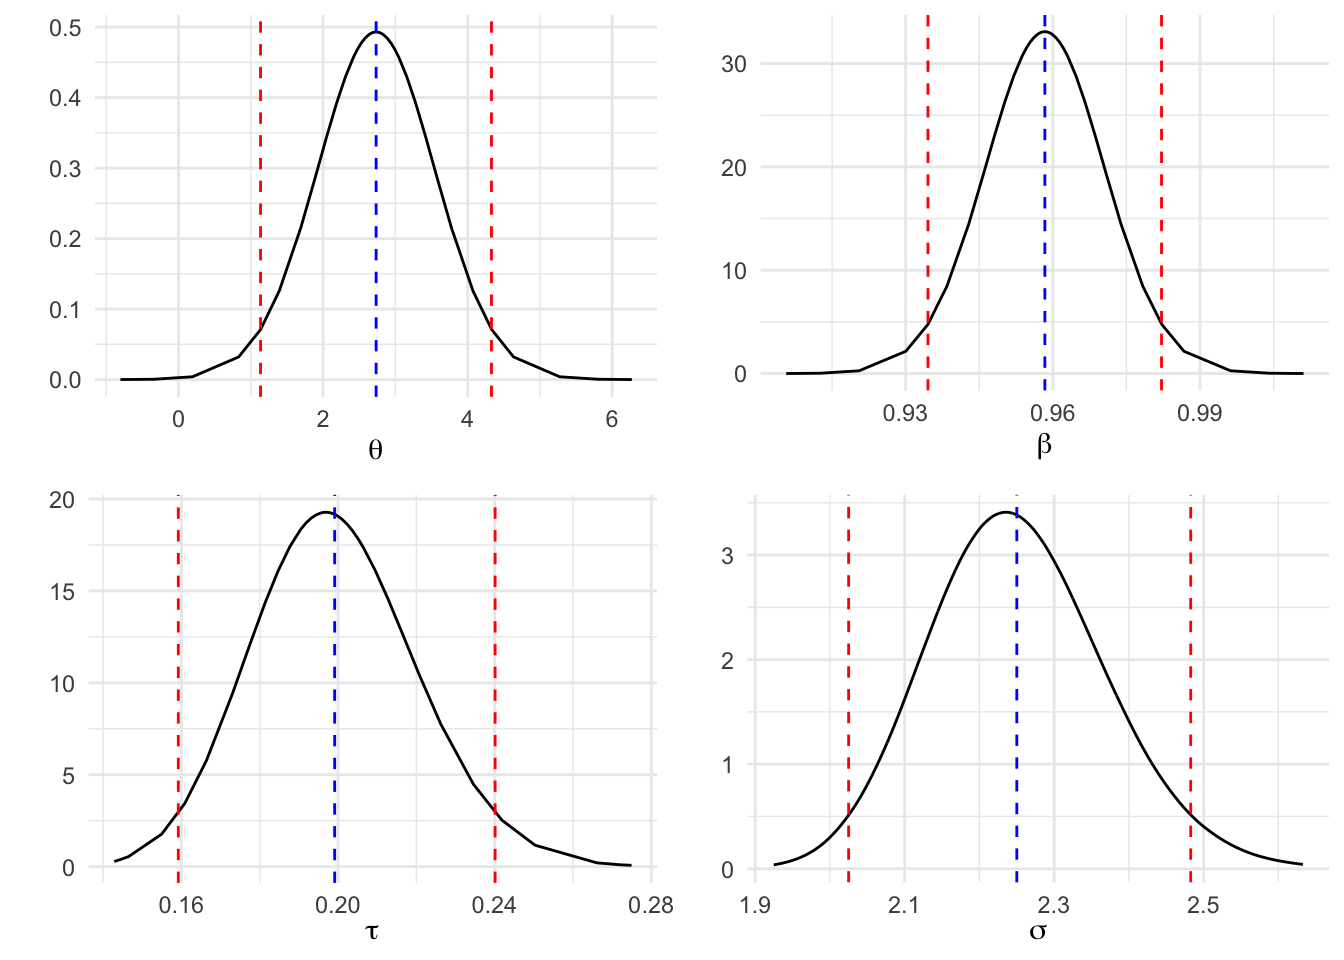
\includegraphics{01-regresion_files/figure-latex/unnamed-chunk-15-1.pdf}

Si queremos la distribución posterior de alguna de las medias \(\mu_i=\theta+ \beta x_i\), necesitamos añadir el argumento \texttt{control.compute=list(return.marginals.predictor=TRUE)} en \texttt{inla}. Así podremos representar, por ejemplo, la distribución posterior sobre el peso esperado para el individuo que aparece en el registro 1 de la base de datos, \(\mu_1=\theta+\beta x_1\):

\begin{Shaded}
\begin{Highlighting}[]
\NormalTok{fit}\OtherTok{=}\FunctionTok{inla}\NormalTok{(formula,}\AttributeTok{family=}\StringTok{"gaussian"}\NormalTok{,}\AttributeTok{data=}\NormalTok{davis,}
         \AttributeTok{control.compute=}\FunctionTok{list}\NormalTok{(}\AttributeTok{return.marginals.predictor=}\ConstantTok{TRUE}\NormalTok{))}
\FunctionTok{ggplot}\NormalTok{(}\FunctionTok{as.data.frame}\NormalTok{(fit}\SpecialCharTok{$}\NormalTok{marginals.fitted.values[[}\DecValTok{1}\NormalTok{]]),}\FunctionTok{aes}\NormalTok{(}\AttributeTok{x=}\NormalTok{x,}\AttributeTok{y=}\NormalTok{y))}\SpecialCharTok{+}
  \FunctionTok{geom\_line}\NormalTok{()}\SpecialCharTok{+}
  \FunctionTok{labs}\NormalTok{(}\AttributeTok{x=}\FunctionTok{expression}\NormalTok{(mu[}\DecValTok{1}\NormalTok{]),}\AttributeTok{y=}\StringTok{"D.Posterior"}\NormalTok{)}
\end{Highlighting}
\end{Shaded}

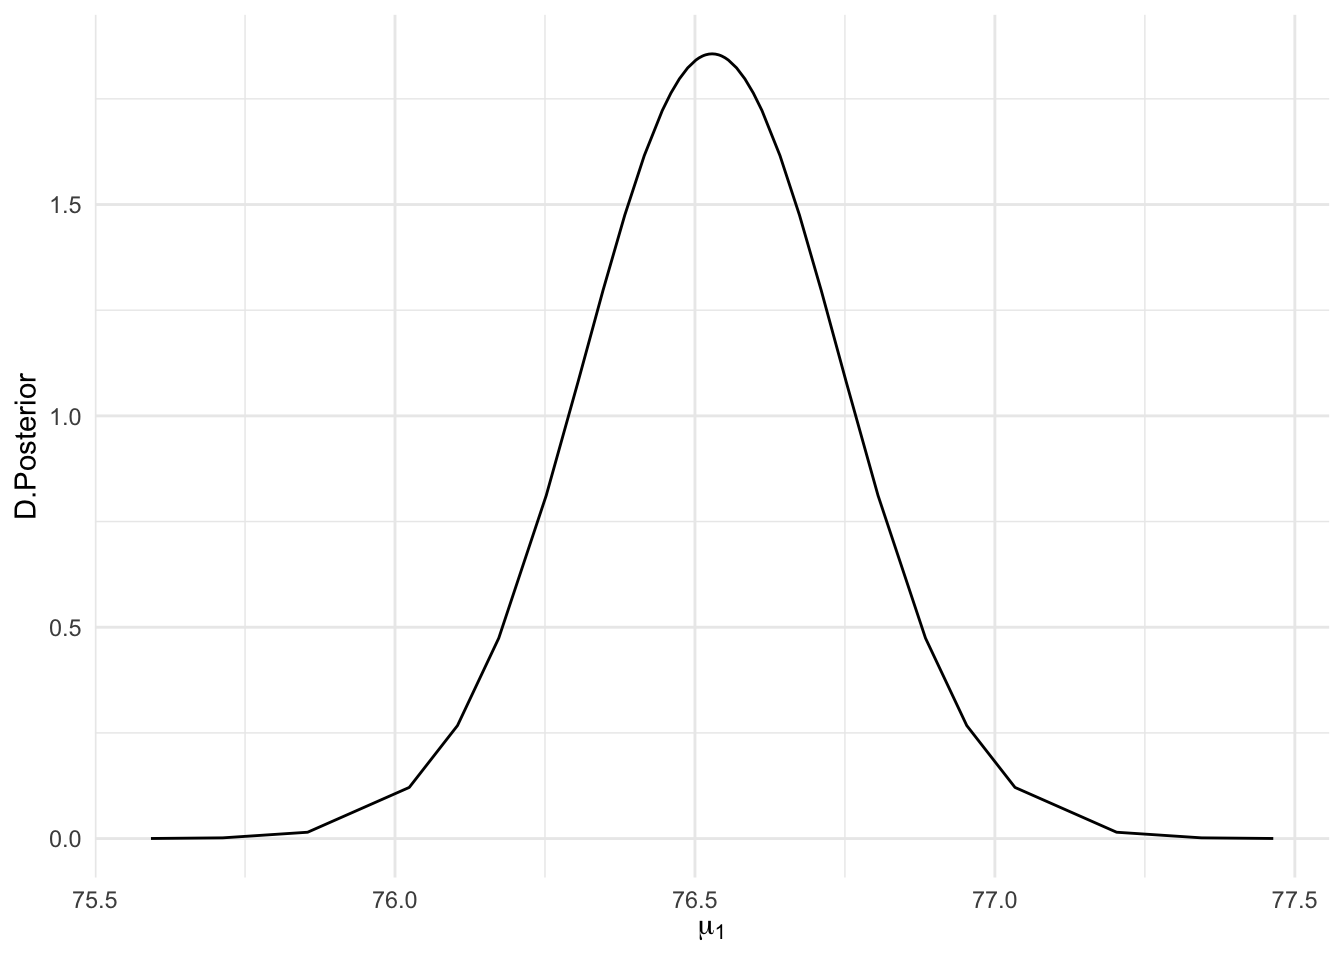
\includegraphics{01-regresion_files/figure-latex/unnamed-chunk-16-1.pdf}

\hypertarget{simulaciuxf3n-de-la-posterior}{%
\section{Simulación de la posterior}\label{simulaciuxf3n-de-la-posterior}}

Cuando queremos inferir sobre funciones de los efectos latentes e hiperparámetros que no proporciona \texttt{INLA} por defecto , podemos recurrir a simular de las distribuciones posteriores de los efectos involucrados, y con ellas evaluar la función que nos interesa, para conseguir una muestra de su distribución posterior.

Para ello es preciso que al ajustar el modelo con \texttt{inla} hayamos incluido el argumento \texttt{control.compute=list(config=TRUE)}.

Para obtener simulaciones de las correspondientes distribuciones posteriores, utilizamos las funciones:

\begin{itemize}
\tightlist
\item
  \texttt{inla.posterior.sample(n,\ fit,selection)}, para simular los efectos latentes, donde \(n\) es el número de simulaciones pretendido, \texttt{fit} es el ajuste obtenido con \texttt{inla} y \texttt{selection} es una lista con el nombre de las componentes (efectos latentes) a simular.\\
\item
  \texttt{inla.hyperpar.sample(n,fit,improve.marginals=TRUE)} para simular de parámetros e hiperparámetros.
\end{itemize}

Para describir las distribuciones de los nuevos parámetros que queremos evaluar con dichas simulaciones, utilizaremos:

\begin{itemize}
\tightlist
\item
  \texttt{inla.posterior.eval()} para funciones sobre los efectos fijos
\item
  \texttt{inla.hyperpar.eval()} para funciones sobre los hiperparámetros
\end{itemize}

Imaginemos que queremos obtener la distribución posterior de \((\theta+\beta \cdot 50)\), que correspondería con el peso real de un sujeto que ha declarado un peso de 50kg. Hemos de simular pues, de las distribuciones posteriores de \(\theta\) y de \(\beta\), para luego aplicar la función correspondiente sobre las simulaciones y obtener una muestra posterior de \(\theta+\beta\cdot 50\).

\begin{Shaded}
\begin{Highlighting}[]
\CommentTok{\# reajustamos para poder simular de las posterioris}
\NormalTok{fit }\OtherTok{\textless{}{-}} \FunctionTok{inla}\NormalTok{(formula, }\AttributeTok{data =}\NormalTok{ davis,}
  \AttributeTok{control.compute =} \FunctionTok{list}\NormalTok{(}\AttributeTok{config =} \ConstantTok{TRUE}\NormalTok{))}
\CommentTok{\# simulamos especificando los parámetros en los que tenemos interés}
\NormalTok{sims }\OtherTok{=} \FunctionTok{inla.posterior.sample}\NormalTok{(}\DecValTok{100}\NormalTok{, fit, }\AttributeTok{selection =} \FunctionTok{list}\NormalTok{(}\StringTok{"(Intercept)"}\OtherTok{=}\DecValTok{1}\NormalTok{,}\AttributeTok{repwt =} \DecValTok{1}\NormalTok{))}
\end{Highlighting}
\end{Shaded}

Esto nos devuelve una lista de la dimensión del número de simulaciones (cada simulación en un elemento de la lista), y en cada uno de los elementos tenemos los valores simulados de los hiperparámetros (\texttt{hyper}), de los efectos latentes (\texttt{latent})

\begin{Shaded}
\begin{Highlighting}[]
\FunctionTok{length}\NormalTok{(sims)}
\CommentTok{\#\textgreater{} [1] 100}
\FunctionTok{names}\NormalTok{(sims[[}\DecValTok{1}\NormalTok{]])}
\CommentTok{\#\textgreater{} [1] "hyperpar" "latent"   "logdens"}
\NormalTok{sims[[}\DecValTok{1}\NormalTok{]]}\SpecialCharTok{$}\NormalTok{hyperpar}
\CommentTok{\#\textgreater{} Precision for the Gaussian observations }
\CommentTok{\#\textgreater{}                                0.215942}
\NormalTok{sims[[}\DecValTok{1}\NormalTok{]]}\SpecialCharTok{$}\NormalTok{latent}
\CommentTok{\#\textgreater{}                sample:1}
\CommentTok{\#\textgreater{} (Intercept):1 3.6452565}
\CommentTok{\#\textgreater{} repwt:1       0.9483437}
\end{Highlighting}
\end{Shaded}

y la log-densidad de la posterior en esos valores (\texttt{logdens})

\begin{Shaded}
\begin{Highlighting}[]
\NormalTok{ sims[[}\DecValTok{1}\NormalTok{]]}\SpecialCharTok{$}\NormalTok{logdens}
\CommentTok{\#\textgreater{} $hyperpar}
\CommentTok{\#\textgreater{} [1] 2.561111}
\CommentTok{\#\textgreater{} }
\CommentTok{\#\textgreater{} $latent}
\CommentTok{\#\textgreater{} [1] 1008.692}
\CommentTok{\#\textgreater{} }
\CommentTok{\#\textgreater{} $joint}
\CommentTok{\#\textgreater{} [1] 1011.253}
\end{Highlighting}
\end{Shaded}

Ahora con la función \texttt{inla.posterior.sample.eval}, dado que nuestra función depende de efectos fijos (latentes), \((\theta,\beta)\), evaluamos la operación pretendida, y con descriptivos gráficos y numéricos de las simulaciones, podemos aproximar los descriptivos de la distribución posterior.

\begin{Shaded}
\begin{Highlighting}[]
\NormalTok{peso\_real}\OtherTok{=}\FunctionTok{inla.posterior.sample.eval}\NormalTok{(}\ControlFlowTok{function}\NormalTok{(...) \{(Intercept)}\SpecialCharTok{+}\NormalTok{repwt}\SpecialCharTok{*}\DecValTok{50}\NormalTok{\},sims)}
\NormalTok{peso\_real}
\CommentTok{\#\textgreater{}        sample:1 sample:2 sample:3 sample:4 sample:5}
\CommentTok{\#\textgreater{} fun[1] 51.06244 50.52529 50.70436 50.22757 50.34733}
\CommentTok{\#\textgreater{}        sample:6 sample:7 sample:8 sample:9 sample:10}
\CommentTok{\#\textgreater{} fun[1] 50.44512   51.092 50.70692  50.9964  50.99253}
\CommentTok{\#\textgreater{}        sample:11 sample:12 sample:13 sample:14 sample:15}
\CommentTok{\#\textgreater{} fun[1]  50.69731  50.47479  50.89714   51.0874  50.72708}
\CommentTok{\#\textgreater{}        sample:16 sample:17 sample:18 sample:19 sample:20}
\CommentTok{\#\textgreater{} fun[1]  50.78735  50.80462  50.43316  50.80696  50.65538}
\CommentTok{\#\textgreater{}        sample:21 sample:22 sample:23 sample:24 sample:25}
\CommentTok{\#\textgreater{} fun[1]  51.30029  50.51282  50.91033  50.50204  50.64499}
\CommentTok{\#\textgreater{}        sample:26 sample:27 sample:28 sample:29 sample:30}
\CommentTok{\#\textgreater{} fun[1]  50.36004  50.64481  50.61538   50.8281  50.33711}
\CommentTok{\#\textgreater{}        sample:31 sample:32 sample:33 sample:34 sample:35}
\CommentTok{\#\textgreater{} fun[1]  50.93313  50.19321  51.21467  50.87816  50.69253}
\CommentTok{\#\textgreater{}        sample:36 sample:37 sample:38 sample:39 sample:40}
\CommentTok{\#\textgreater{} fun[1]  50.93738  50.24804   50.4517   50.7124  50.78072}
\CommentTok{\#\textgreater{}        sample:41 sample:42 sample:43 sample:44 sample:45}
\CommentTok{\#\textgreater{} fun[1]  50.13386  50.89244  50.18202  50.84824   50.6755}
\CommentTok{\#\textgreater{}        sample:46 sample:47 sample:48 sample:49 sample:50}
\CommentTok{\#\textgreater{} fun[1]  50.86679  50.65348  50.61743  50.51478  50.36984}
\CommentTok{\#\textgreater{}        sample:51 sample:52 sample:53 sample:54 sample:55}
\CommentTok{\#\textgreater{} fun[1]  50.55761  50.71592    50.626  51.02911  50.18379}
\CommentTok{\#\textgreater{}        sample:56 sample:57 sample:58 sample:59 sample:60}
\CommentTok{\#\textgreater{} fun[1]  51.20378  50.83704  50.54454  50.40454  50.67299}
\CommentTok{\#\textgreater{}        sample:61 sample:62 sample:63 sample:64 sample:65}
\CommentTok{\#\textgreater{} fun[1]   50.3547   50.3291  50.73312  50.34969  50.40699}
\CommentTok{\#\textgreater{}        sample:66 sample:67 sample:68 sample:69 sample:70}
\CommentTok{\#\textgreater{} fun[1]  50.51819  50.24715  50.54578  50.35828  50.17157}
\CommentTok{\#\textgreater{}        sample:71 sample:72 sample:73 sample:74 sample:75}
\CommentTok{\#\textgreater{} fun[1]  50.51734  50.56676  50.64262  50.57489  50.55392}
\CommentTok{\#\textgreater{}        sample:76 sample:77 sample:78 sample:79 sample:80}
\CommentTok{\#\textgreater{} fun[1]   50.6588   50.6248  50.38832  50.94177  50.52546}
\CommentTok{\#\textgreater{}        sample:81 sample:82 sample:83 sample:84 sample:85}
\CommentTok{\#\textgreater{} fun[1]  50.33435  50.55521  50.83632   50.6393  49.94654}
\CommentTok{\#\textgreater{}        sample:86 sample:87 sample:88 sample:89 sample:90}
\CommentTok{\#\textgreater{} fun[1]  50.39626  50.88559  50.01248  50.65951  50.24457}
\CommentTok{\#\textgreater{}        sample:91 sample:92 sample:93 sample:94 sample:95}
\CommentTok{\#\textgreater{} fun[1]   50.5403  50.63917  50.59824  50.41855  50.41156}
\CommentTok{\#\textgreater{}        sample:96 sample:97 sample:98 sample:99 sample:100}
\CommentTok{\#\textgreater{} fun[1]   50.7114   50.5354  50.87874  50.56769   50.17803}
\NormalTok{pred}\OtherTok{=}\FunctionTok{data.frame}\NormalTok{(}\AttributeTok{peso=}\FunctionTok{as.vector}\NormalTok{(peso\_real))}
\FunctionTok{summary}\NormalTok{(pred)}
\CommentTok{\#\textgreater{}       peso      }
\CommentTok{\#\textgreater{}  Min.   :49.95  }
\CommentTok{\#\textgreater{}  1st Qu.:50.41  }
\CommentTok{\#\textgreater{}  Median :50.62  }
\CommentTok{\#\textgreater{}  Mean   :50.61  }
\CommentTok{\#\textgreater{}  3rd Qu.:50.79  }
\CommentTok{\#\textgreater{}  Max.   :51.30}
\FunctionTok{ggplot}\NormalTok{(pred,}\FunctionTok{aes}\NormalTok{(}\AttributeTok{x=}\NormalTok{peso))}\SpecialCharTok{+}
  \FunctionTok{geom\_histogram}\NormalTok{(}\FunctionTok{aes}\NormalTok{(}\AttributeTok{y=}\NormalTok{..density..), }\AttributeTok{colour=}\StringTok{"black"}\NormalTok{, }\AttributeTok{fill=}\StringTok{"white"}\NormalTok{)}\SpecialCharTok{+}
  \FunctionTok{geom\_density}\NormalTok{(}\AttributeTok{alpha=}\NormalTok{.}\DecValTok{2}\NormalTok{, }\AttributeTok{fill=}\StringTok{"\#80E7F5"}\NormalTok{) }
\CommentTok{\#\textgreater{} \textasciigrave{}stat\_bin()\textasciigrave{} using \textasciigrave{}bins = 30\textasciigrave{}. Pick better value with}
\CommentTok{\#\textgreater{} \textasciigrave{}binwidth\textasciigrave{}.}
\end{Highlighting}
\end{Shaded}

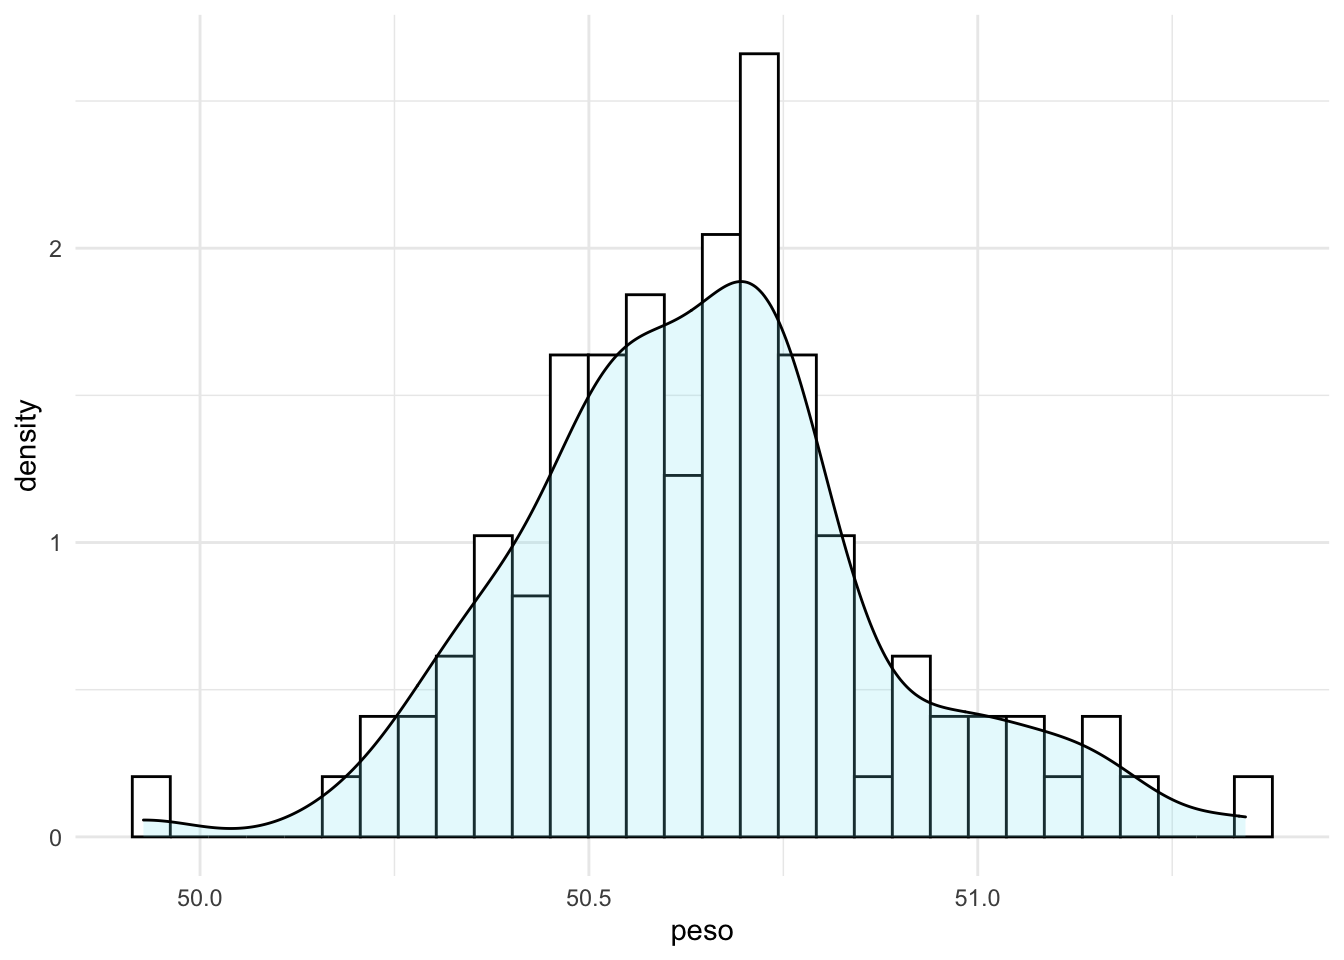
\includegraphics{01-regresion_files/figure-latex/unnamed-chunk-20-1.pdf}

\hypertarget{regresiuxf3n-lineal-muxfaltiple-con-inla}{%
\section{Regresión lineal múltiple con INLA}\label{regresiuxf3n-lineal-muxfaltiple-con-inla}}

Vemos a continuación cómo se trabaja la regresión múltiple con INLA, simplemente añadiendo más predictores.

El modelo de regresión asume una distribución normal para los datos, datos los efectos latentes (todos los relacionados con el valor esperado o predictor lineal) y el resto de parámetros o hiperparámetros del modelo (en nuestro caso la varianza de los datos).

Si tenemos \(n\) observaciones
\[ (y_i|\mu_i,\sigma^2) \sim N(\mu_i,\sigma^2), \ \ i=1,...n\]
donde \(\mu_i\) representa la media y \(\sigma^2\) la varianza de los datos.
\[E(y_i|\mu_i,\sigma^2)=\mu_i, \ Var(y_i|\mu_i,\sigma^2)=\sigma^2\]
Si tenemos varios regresores \(x_1,x_2,...,x_J\), la media \(\mu_i\) coincide con el predictor lineal \(\eta_i\) que se construye a partir de una combinación lineal de los predictores:
\[\mu_i=\eta_i=\theta+ \sum_{j=1}^J \beta_j x_{ij}\]
Nos queda a continuación especificar las distribuciones a priori sobre el vector de efectos latentes, en nuestro caso efectos fijos, \((\theta,\beta_1,...,\beta_J)\), y sobre el parámetro de dispersión o hiperparámetro \(\sigma^2\).

Cuando no tenemos información previa especificamos distribuciones difusas (vagas) sobre los parámetros. En INLA por defecto tendremos:

\begin{eqnarray*}
\theta &\sim& N(0,\sigma_{\theta}^2)  \\
\beta_j &\sim& N(0,\sigma_{\beta}^2) \\
log(\tau=1/\sigma^2) &\sim& Log-Ga(1,0.00005)
\end{eqnarray*}
con \(\sigma_{\theta}^2=\infty\) y \(\sigma_{\beta}^2=1000\).

Ejemplificamos el análisis de regresión lineal múltiple sobre la base de datos \texttt{usair}, en la librería \texttt{brinla}. Esta BD contiene datos recopilados para investigar los factores determinantes de la polución, utilizando el nivel de SO2 como variable dependiente y las restantes como variables explicativas potenciales. Las relaciones entre las variables que incluye se muestra en la Figura \ref{fig:regmul01} a continuación.

\begin{Shaded}
\begin{Highlighting}[]
\FunctionTok{data}\NormalTok{(usair, }\AttributeTok{package =} \StringTok{"brinla"}\NormalTok{)}
\FunctionTok{library}\NormalTok{(GGally) }\CommentTok{\# contiene la función de graficado \textquotesingle{}ggpairs\textquotesingle{}}
\NormalTok{pairs.chart }\OtherTok{\textless{}{-}} \FunctionTok{ggpairs}\NormalTok{(usair, }\AttributeTok{lower =} \FunctionTok{list}\NormalTok{(}\AttributeTok{continuous =} \StringTok{"cor"}\NormalTok{), }
                       \AttributeTok{upper =} \FunctionTok{list}\NormalTok{(}\AttributeTok{continuous =} \StringTok{"points"}\NormalTok{, }\AttributeTok{combo =} \StringTok{"dot"}\NormalTok{))}
\NormalTok{ggplot2}\SpecialCharTok{::}\FunctionTok{theme}\NormalTok{(}\AttributeTok{axis.text =} \FunctionTok{element\_text}\NormalTok{(}\AttributeTok{size =} \DecValTok{6}\NormalTok{)) }
\CommentTok{\#\textgreater{} List of 1}
\CommentTok{\#\textgreater{}  $ axis.text:List of 11}
\CommentTok{\#\textgreater{}   ..$ family       : NULL}
\CommentTok{\#\textgreater{}   ..$ face         : NULL}
\CommentTok{\#\textgreater{}   ..$ colour       : NULL}
\CommentTok{\#\textgreater{}   ..$ size         : num 6}
\CommentTok{\#\textgreater{}   ..$ hjust        : NULL}
\CommentTok{\#\textgreater{}   ..$ vjust        : NULL}
\CommentTok{\#\textgreater{}   ..$ angle        : NULL}
\CommentTok{\#\textgreater{}   ..$ lineheight   : NULL}
\CommentTok{\#\textgreater{}   ..$ margin       : NULL}
\CommentTok{\#\textgreater{}   ..$ debug        : NULL}
\CommentTok{\#\textgreater{}   ..$ inherit.blank: logi FALSE}
\CommentTok{\#\textgreater{}   ..{-} attr(*, "class")= chr [1:2] "element\_text" "element"}
\CommentTok{\#\textgreater{}  {-} attr(*, "class")= chr [1:2] "theme" "gg"}
\CommentTok{\#\textgreater{}  {-} attr(*, "complete")= logi FALSE}
\CommentTok{\#\textgreater{}  {-} attr(*, "validate")= logi TRUE}
\NormalTok{pairs.chart}
\end{Highlighting}
\end{Shaded}

\begin{figure}
\centering
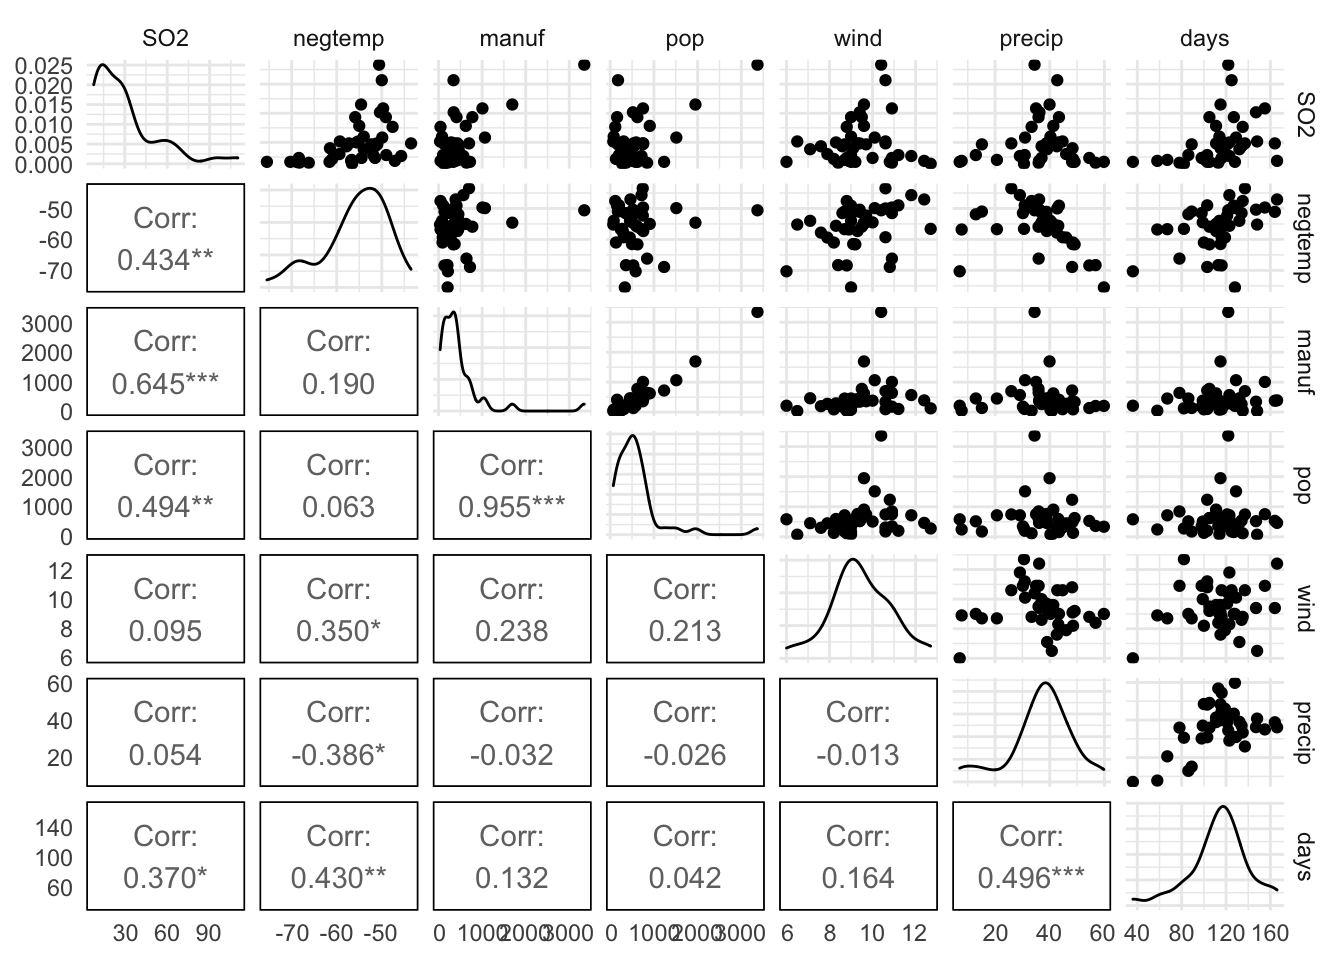
\includegraphics{01-regresion_files/figure-latex/regmul01-1.pdf}
\caption{\label{fig:regmul01}Relaciones entre variables en la base de datos usair(brinla).}
\end{figure}

Apreciamos ya en el gráfico una correlación positiva muy alta entre las variables \texttt{pop} y \texttt{manuf}, y relevante para \texttt{negtemp} y \texttt{days} y también para \texttt{precip} y \texttt{days}, lo que posteriormente condicionará la selección de variables.

\hypertarget{selecciuxf3n-de-variables}{%
\subsection{Selección de variables}\label{selecciuxf3n-de-variables}}

Cuando trabajamos con más de una variable predictora en regresión lineal (realmente en cualquier modelo) surge un problema adicional, que es la \textbf{selección de variables}, o selección del mejor modelo de predicción. Esto se resuelve en INLA utilizando diversos criterios de selección entre los que destacamos:

\begin{itemize}
\tightlist
\item
  la verosimilitud marginal (valor de la log-verosimilitud): \texttt{mlik}; al cambiarle el signo tendremos \emph{-(log-likelihood)}
\item
  el criterio de información de la deviance (DIC): \texttt{dic}
\item
  el criterio de información bayesiana ampliado (WAIC): \texttt{waic}
\item
  la transformada integral predictiva (PIT): \texttt{cpo}
\end{itemize}

El procedimiento a utilizar para la selección del modelo (de variables) es el siguiente:

\begin{enumerate}
\def\labelenumi{\arabic{enumi}.}
\tightlist
\item
  ajustar todos los modelos resultantes de todas las combinaciones posibles de predictoras,
\item
  calcular los índices de selección para cada uno de ellos
\item
  proceder con la selección en base a dichos valores.
\end{enumerate}

Siempre se prefieren modelos con los valores más bajos para estos criterios y se descartan los que proporcionan valores más altos. Cuando no es el mismo modelo el que proporciona el valor mínimo en estos criterios, habremos de optar por alguno de ellos.

Por defecto, al ajustar un modelo con \texttt{inla}, nos devuelve la log-verosimilitud marginal (accesible con \texttt{fit\$mlik} si el ajuste se guardó en el objeto \texttt{fit}). Para obtener las otras medidas de selección, hemos de incluir como argumento de la función \texttt{inla}, la opción \texttt{control.compute\ =\ list(dic\ =\ TRUE,\ waic\ =\ TRUE))}. Los valores por defecto de \texttt{control.compute} los podemos consultar ejecutando el comando \texttt{inla.set.control.compute.default()}.

Vayamos pues con el ajuste del modelo de regresión con todas las variables. Recordemos que si no especificamos el argumento \texttt{family}, interpreta por defecto la opción \texttt{gaussian}, esto es, normalidad para los datos. Así ajustamos el modelo y obtenemos las siguientes inferencias sobre los efectos fijos.

\begin{Shaded}
\begin{Highlighting}[]
\NormalTok{formula }\OtherTok{\textless{}{-}}\NormalTok{  SO2 }\SpecialCharTok{\textasciitilde{}}\NormalTok{ negtemp }\SpecialCharTok{+}\NormalTok{ manuf }\SpecialCharTok{+}\NormalTok{ wind }\SpecialCharTok{+}\NormalTok{ precip }\SpecialCharTok{+}\NormalTok{ days}
\NormalTok{fit}\OtherTok{=} \FunctionTok{inla}\NormalTok{(formula, }\AttributeTok{data =}\NormalTok{ usair, }
          \AttributeTok{control.compute =} \FunctionTok{list}\NormalTok{(}\AttributeTok{dic =} \ConstantTok{TRUE}\NormalTok{, }\AttributeTok{waic =} \ConstantTok{TRUE}\NormalTok{))}
\CommentTok{\#summary(fit)}
\FunctionTok{round}\NormalTok{(fit}\SpecialCharTok{$}\NormalTok{summary.fixed,}\DecValTok{3}\NormalTok{)}
\CommentTok{\#\textgreater{}                mean     sd 0.025quant 0.5quant 0.975quant}
\CommentTok{\#\textgreater{} (Intercept) 135.489 49.862     37.153  135.496    233.784}
\CommentTok{\#\textgreater{} negtemp       1.769  0.634      0.518    1.769      3.020}
\CommentTok{\#\textgreater{} manuf         0.026  0.005      0.017    0.026      0.035}
\CommentTok{\#\textgreater{} wind         {-}3.723  1.935     {-}7.537   {-}3.723      0.093}
\CommentTok{\#\textgreater{} precip        0.625  0.387     {-}0.139    0.625      1.388}
\CommentTok{\#\textgreater{} days         {-}0.057  0.174     {-}0.400   {-}0.057      0.287}
\CommentTok{\#\textgreater{}             mode kld}
\CommentTok{\#\textgreater{} (Intercept)   NA   0}
\CommentTok{\#\textgreater{} negtemp       NA   0}
\CommentTok{\#\textgreater{} manuf         NA   0}
\CommentTok{\#\textgreater{} wind          NA   0}
\CommentTok{\#\textgreater{} precip        NA   0}
\CommentTok{\#\textgreater{} days          NA   0}
\end{Highlighting}
\end{Shaded}

La inferencia posterior sobre la desviación típica de los datos, \(\sigma\), la resolvemos con sus descriptivos.

\begin{Shaded}
\begin{Highlighting}[]
\NormalTok{sigma.post}\OtherTok{=} \FunctionTok{inla.tmarginal}\NormalTok{(}\ControlFlowTok{function}\NormalTok{(tau) tau}\SpecialCharTok{\^{}}\NormalTok{(}\SpecialCharTok{{-}}\DecValTok{1}\SpecialCharTok{/}\DecValTok{2}\NormalTok{),}
\NormalTok{                           fit}\SpecialCharTok{$}\NormalTok{marginals.hyperpar[[}\DecValTok{1}\NormalTok{]])}
\FunctionTok{inla.zmarginal}\NormalTok{(sigma.post)}
\CommentTok{\#\textgreater{} Mean            15.6719 }
\CommentTok{\#\textgreater{} Stdev           1.85609 }
\CommentTok{\#\textgreater{} Quantile  0.025 12.5298 }
\CommentTok{\#\textgreater{} Quantile  0.25  14.3479 }
\CommentTok{\#\textgreater{} Quantile  0.5   15.4936 }
\CommentTok{\#\textgreater{} Quantile  0.75  16.7992 }
\CommentTok{\#\textgreater{} Quantile  0.975 19.8195}
\end{Highlighting}
\end{Shaded}

Para seleccionar las variables relevantes seguimos el procedimiento descrito anteriormente. Añadimos también el ajuste del modelo de regresión frecuentista, para el que calculamos como criterio de bondad de ajuste el AIC.

\begin{Shaded}
\begin{Highlighting}[]
\CommentTok{\# variables en la bd}
\NormalTok{vars}\OtherTok{=}\FunctionTok{names}\NormalTok{(usair)[}\SpecialCharTok{{-}}\DecValTok{1}\NormalTok{] }\CommentTok{\# variables predictoras (excluye v.dpte)}
\NormalTok{nvars}\OtherTok{=}\FunctionTok{length}\NormalTok{(vars) }\CommentTok{\# nº variables predictoras}

\CommentTok{\# Truco para concatenar todos los modelos posibles en una fórmula (de Faraway)}
\NormalTok{listcombo }\OtherTok{\textless{}{-}} \FunctionTok{unlist}\NormalTok{(}\FunctionTok{sapply}\NormalTok{(}\DecValTok{1}\SpecialCharTok{:}\NormalTok{nvars,}
                           \ControlFlowTok{function}\NormalTok{(x) }\FunctionTok{combn}\NormalTok{(nvars, x, }\AttributeTok{simplify=}\ConstantTok{FALSE}\NormalTok{)),}
                    \AttributeTok{recursive=}\ConstantTok{FALSE}\NormalTok{)}
\NormalTok{predterms }\OtherTok{\textless{}{-}} \FunctionTok{lapply}\NormalTok{(listcombo, }
                    \ControlFlowTok{function}\NormalTok{(x) }\FunctionTok{paste}\NormalTok{(vars[x],}\AttributeTok{collapse=}\StringTok{"+"}\NormalTok{))}
\NormalTok{nmodels }\OtherTok{\textless{}{-}} \FunctionTok{length}\NormalTok{(listcombo)}
\NormalTok{coefm }\OtherTok{\textless{}{-}} \FunctionTok{matrix}\NormalTok{(}\ConstantTok{NA}\NormalTok{,}\FunctionTok{length}\NormalTok{(listcombo),}\DecValTok{4}\NormalTok{,}
                \AttributeTok{dimnames=}\FunctionTok{list}\NormalTok{(predterms,}\FunctionTok{c}\NormalTok{(}\StringTok{"AIC"}\NormalTok{,}\StringTok{"DIC"}\NormalTok{,}\StringTok{"WAIC"}\NormalTok{,}\StringTok{"MLIK"}\NormalTok{)))}

\CommentTok{\# Ajuste de todos los modelos posibles}
\ControlFlowTok{for}\NormalTok{(i }\ControlFlowTok{in} \DecValTok{1}\SpecialCharTok{:}\NormalTok{nmodels)\{}
\NormalTok{  formula }\OtherTok{\textless{}{-}} \FunctionTok{as.formula}\NormalTok{(}\FunctionTok{paste}\NormalTok{(}\StringTok{"SO2 \textasciitilde{} "}\NormalTok{,predterms[[i]]))}
  \CommentTok{\# modelo frecuentista}
\NormalTok{  lmi }\OtherTok{\textless{}{-}} \FunctionTok{lm}\NormalTok{(formula, }\AttributeTok{data=}\NormalTok{usair)}
  \CommentTok{\# modelo bayesiano}
\NormalTok{  result }\OtherTok{\textless{}{-}} \FunctionTok{inla}\NormalTok{(formula, }\AttributeTok{family=}\StringTok{"gaussian"}\NormalTok{, }\AttributeTok{data=}\NormalTok{usair, }\AttributeTok{control.compute=}\FunctionTok{list}\NormalTok{(}\AttributeTok{dic=}\ConstantTok{TRUE}\NormalTok{, }\AttributeTok{waic=}\ConstantTok{TRUE}\NormalTok{))}
\NormalTok{  coefm[i,}\DecValTok{1}\NormalTok{] }\OtherTok{\textless{}{-}} \FunctionTok{AIC}\NormalTok{(lmi)}
\NormalTok{  coefm[i,}\DecValTok{2}\NormalTok{] }\OtherTok{\textless{}{-}}\NormalTok{ result}\SpecialCharTok{$}\NormalTok{dic}\SpecialCharTok{$}\NormalTok{dic}
\NormalTok{  coefm[i,}\DecValTok{3}\NormalTok{] }\OtherTok{\textless{}{-}}\NormalTok{ result}\SpecialCharTok{$}\NormalTok{waic}\SpecialCharTok{$}\NormalTok{waic}
\NormalTok{  coefm[i,}\DecValTok{4}\NormalTok{] }\OtherTok{\textless{}{-}} \SpecialCharTok{{-}}\NormalTok{result}\SpecialCharTok{$}\NormalTok{mlik[}\DecValTok{1}\NormalTok{]}
\NormalTok{\}}
\end{Highlighting}
\end{Shaded}

Ya solo resta comparar los resultados, respecto de cada uno de los criterios, para seleccionar con qué variables nos quedamos, y por lo tanto con qué modelo de predicción. Basta con encontrar el modelo que proporciona el mínimo valor en cada uno de los criterios.

\begin{Shaded}
\begin{Highlighting}[]
\NormalTok{gana.aic }\OtherTok{=}\NormalTok{ predterms[}\FunctionTok{which.min}\NormalTok{(coefm[,}\DecValTok{1}\NormalTok{])]}
\NormalTok{gana.dic }\OtherTok{=}\NormalTok{ predterms[}\FunctionTok{which.min}\NormalTok{(coefm[,}\DecValTok{2}\NormalTok{])]}
\NormalTok{gana.waic }\OtherTok{=}\NormalTok{ predterms[}\FunctionTok{which.min}\NormalTok{(coefm[,}\DecValTok{3}\NormalTok{])]}
\NormalTok{gana.mlik }\OtherTok{=}\NormalTok{ predterms[}\FunctionTok{which.min}\NormalTok{(coefm[,}\DecValTok{4}\NormalTok{])]}
\NormalTok{gana.aic;gana.dic}
\CommentTok{\#\textgreater{} [[1]]}
\CommentTok{\#\textgreater{} [1] "negtemp+manuf+pop+wind+precip"}
\CommentTok{\#\textgreater{} [[1]]}
\CommentTok{\#\textgreater{} [1] "negtemp+manuf+pop+wind+precip"}
\NormalTok{gana.waic;gana.mlik}
\CommentTok{\#\textgreater{} [[1]]}
\CommentTok{\#\textgreater{} [1] "negtemp+manuf+pop+wind+precip"}
\CommentTok{\#\textgreater{} [[1]]}
\CommentTok{\#\textgreater{} [1] "manuf"}
\end{Highlighting}
\end{Shaded}

Concluimos pues que, tanto el criterio AIC en el modelo de regresión frecuentista, como los criterios DIC y WAIC en el modelo de regresión bayesiano, proporcionan el mejor ajuste. Este mejor modelo incluye como predictores las variables `negtemp+manuf+pop+wind+precip'. Reajustamos el modelo con estas variables para derivar las inferencias y predicciones.

Las inferencias sobre los efectos fijos y la precisión de los datos se muestran a continuación.

\begin{Shaded}
\begin{Highlighting}[]
\NormalTok{formula}\OtherTok{=}\NormalTok{SO2 }\SpecialCharTok{\textasciitilde{}}\NormalTok{ negtemp}\SpecialCharTok{+}\NormalTok{manuf}\SpecialCharTok{+}\NormalTok{pop}\SpecialCharTok{+}\NormalTok{wind}\SpecialCharTok{+}\NormalTok{precip}
\NormalTok{fit}\OtherTok{=}\FunctionTok{inla}\NormalTok{(formula, }\AttributeTok{family=}\StringTok{"gaussian"}\NormalTok{, }\AttributeTok{data=}\NormalTok{usair, }\AttributeTok{control.compute=}\FunctionTok{list}\NormalTok{(}\AttributeTok{dic=}\ConstantTok{TRUE}\NormalTok{, }\AttributeTok{waic=}\ConstantTok{TRUE}\NormalTok{))}
\NormalTok{fit}\SpecialCharTok{$}\NormalTok{summary.fixed}
\CommentTok{\#\textgreater{}                     mean          sd   0.025quant}
\CommentTok{\#\textgreater{} (Intercept) 100.01507684 30.13792337 40.581810484}
\CommentTok{\#\textgreater{} negtemp       1.12026648  0.41427010  0.303360918}
\CommentTok{\#\textgreater{} manuf         0.06489618  0.01548972  0.034355160}
\CommentTok{\#\textgreater{} pop          {-}0.03934757  0.01488331 {-}0.068694574}
\CommentTok{\#\textgreater{} wind         {-}3.07254481  1.75652267 {-}6.535114234}
\CommentTok{\#\textgreater{} precip        0.41922382  0.21546548 {-}0.005636355}
\CommentTok{\#\textgreater{}                 0.5quant   0.975quant mode          kld}
\CommentTok{\#\textgreater{} (Intercept) 100.01864744 159.42790364   NA 1.157176e{-}08}
\CommentTok{\#\textgreater{} negtemp       1.12029323   1.93701886   NA 1.159988e{-}08}
\CommentTok{\#\textgreater{} manuf         0.06489594   0.09543860   NA 1.161204e{-}08}
\CommentTok{\#\textgreater{} pop          {-}0.03934723  {-}0.01000253   NA 1.161129e{-}08}
\CommentTok{\#\textgreater{} wind         {-}3.07280006   0.39148534   NA 1.154611e{-}08}
\CommentTok{\#\textgreater{} precip        0.41923027   0.84404705   NA 1.160859e{-}08}
\NormalTok{fit}\SpecialCharTok{$}\NormalTok{summary.hyperpar}
\CommentTok{\#\textgreater{}                                                mean}
\CommentTok{\#\textgreater{} Precision for the Gaussian observations 0.005066391}
\CommentTok{\#\textgreater{}                                                  sd}
\CommentTok{\#\textgreater{} Precision for the Gaussian observations 0.001179073}
\CommentTok{\#\textgreater{}                                         0.025quant}
\CommentTok{\#\textgreater{} Precision for the Gaussian observations 0.00303505}
\CommentTok{\#\textgreater{}                                            0.5quant}
\CommentTok{\#\textgreater{} Precision for the Gaussian observations 0.004975893}
\CommentTok{\#\textgreater{}                                          0.975quant mode}
\CommentTok{\#\textgreater{} Precision for the Gaussian observations 0.007618676   NA}
\end{Highlighting}
\end{Shaded}

Y en la Figura \ref{fig:regmul02} se muestran las distribuciones posteriores de todos los efectos latentes (efectos fijos) en el modelo: interceptación y coeficientes de los regresores.

\begin{Shaded}
\begin{Highlighting}[]
\NormalTok{nfixed}\OtherTok{=}\FunctionTok{length}\NormalTok{(fit}\SpecialCharTok{$}\NormalTok{names.fixed)}
\NormalTok{g}\OtherTok{=}\FunctionTok{list}\NormalTok{()}
\ControlFlowTok{for}\NormalTok{(i }\ControlFlowTok{in} \DecValTok{1}\SpecialCharTok{:}\NormalTok{nfixed)\{}
\NormalTok{  g[[i]]}\OtherTok{=}\FunctionTok{ggplot}\NormalTok{(}\FunctionTok{as.data.frame}\NormalTok{(fit}\SpecialCharTok{$}\NormalTok{marginals.fixed[[i]])) }\SpecialCharTok{+} 
    \FunctionTok{geom\_line}\NormalTok{(}\FunctionTok{aes}\NormalTok{(}\AttributeTok{x =}\NormalTok{ x, }\AttributeTok{y =}\NormalTok{ y)) }\SpecialCharTok{+}
    \FunctionTok{labs}\NormalTok{(}\AttributeTok{x=}\NormalTok{fit}\SpecialCharTok{$}\NormalTok{names.fixed[i],}\AttributeTok{y=}\StringTok{""}\NormalTok{)}\SpecialCharTok{+}
    \FunctionTok{geom\_vline}\NormalTok{(}\AttributeTok{xintercept=}\FunctionTok{inla.hpdmarginal}\NormalTok{(}\FloatTok{0.95}\NormalTok{,fit}\SpecialCharTok{$}\NormalTok{marginals.fixed[[i]]),}
               \AttributeTok{linetype=}\StringTok{"dashed"}\NormalTok{,}\AttributeTok{color=}\StringTok{"red"}\NormalTok{)}\SpecialCharTok{+}
    \FunctionTok{geom\_vline}\NormalTok{(}\AttributeTok{xintercept=}\FunctionTok{inla.emarginal}\NormalTok{(}\ControlFlowTok{function}\NormalTok{(x) x,fit}\SpecialCharTok{$}\NormalTok{marginals.fixed[[i]]),}
               \AttributeTok{linetype=}\StringTok{"dashed"}\NormalTok{,}\AttributeTok{color=}\StringTok{"blue"}\NormalTok{)}
\NormalTok{\}}
\FunctionTok{grid.arrange}\NormalTok{(g[[}\DecValTok{1}\NormalTok{]],g[[}\DecValTok{2}\NormalTok{]],g[[}\DecValTok{3}\NormalTok{]],g[[}\DecValTok{4}\NormalTok{]],g[[}\DecValTok{5}\NormalTok{]],g[[}\DecValTok{6}\NormalTok{]],}\AttributeTok{ncol=}\DecValTok{2}\NormalTok{)}
\end{Highlighting}
\end{Shaded}

\begin{figure}
\centering
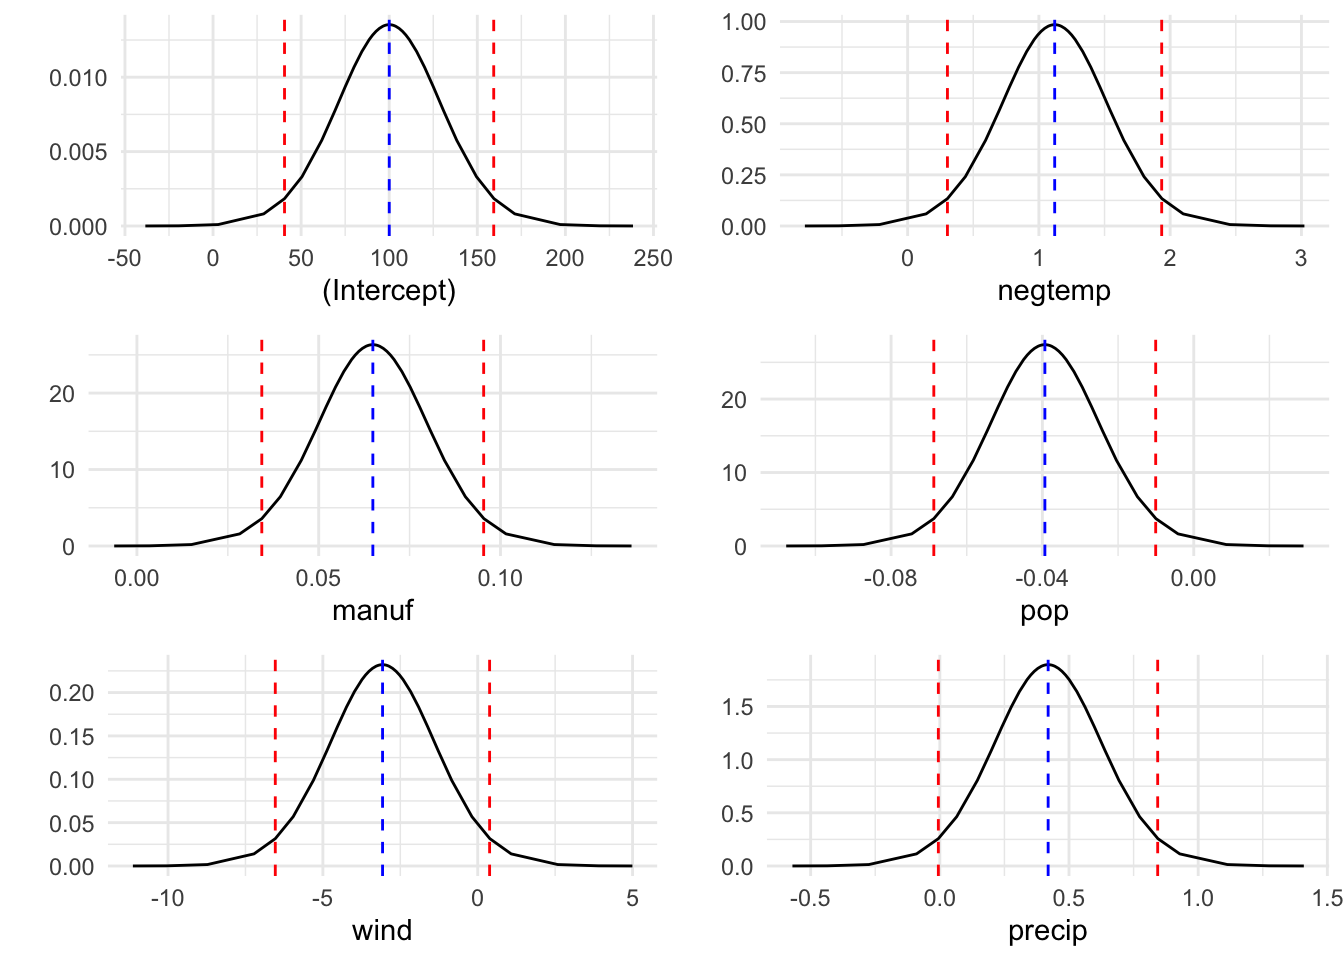
\includegraphics{01-regresion_files/figure-latex/regmul02-1.pdf}
\caption{\label{fig:regmul02}Distribuciones posteriores de los efectos latentes.}
\end{figure}

\hypertarget{predicciuxf3n-de-medias}{%
\subsection{Predicción de medias}\label{predicciuxf3n-de-medias}}

Por último, si queremos predecir la respuesta esperada para ciertos valores de las variables explicativas, no necesariamente existentes en la base de datos, utilizamos el argumento \texttt{control.predictor} en la función \texttt{inla}, especificando en una lista los valores a predecir. Veamos cómo hacerlo con \texttt{inla}, ajustando un modelo sobre un \texttt{data.frame} combinado, en el que añadimos tantas filas como predicciones queremos conseguir, con los valores deseados para los predictores (y valores faltantes en la respuesta), y especificamos los valores a predecir en un vector indicador, a través del argumento \texttt{control.predictor(list(link=vector.indicador))}. Las predicciones se obtienen después, con el resumen de los datos ajustados \texttt{fitted.values}. Recordemos que para poder mostrar las distribuciones predictivas, hemos de añadir en \texttt{inla} el argumento \texttt{control.compute=list(return.marginals.predictor=TRUE)}.

\begin{Shaded}
\begin{Highlighting}[]
\CommentTok{\# Predicción con INLA}
\DocumentationTok{\#\# valores de los predictores en los que predecir: 3 escenarios}
\NormalTok{formula}\OtherTok{=}\NormalTok{SO2 }\SpecialCharTok{\textasciitilde{}}\NormalTok{ negtemp}\SpecialCharTok{+}\NormalTok{manuf}\SpecialCharTok{+}\NormalTok{pop}\SpecialCharTok{+}\NormalTok{wind}\SpecialCharTok{+}\NormalTok{precip}
\NormalTok{new.data }\OtherTok{\textless{}{-}} \FunctionTok{data.frame}\NormalTok{(}\AttributeTok{negtemp =} \FunctionTok{c}\NormalTok{(}\SpecialCharTok{{-}}\DecValTok{50}\NormalTok{, }\SpecialCharTok{{-}}\DecValTok{60}\NormalTok{, }\SpecialCharTok{{-}}\DecValTok{40}\NormalTok{), }
                       \AttributeTok{manuf =} \FunctionTok{c}\NormalTok{(}\DecValTok{150}\NormalTok{, }\DecValTok{100}\NormalTok{, }\DecValTok{400}\NormalTok{), }
                       \AttributeTok{pop =} \FunctionTok{c}\NormalTok{(}\DecValTok{200}\NormalTok{, }\DecValTok{100}\NormalTok{, }\DecValTok{300}\NormalTok{), }
                       \AttributeTok{wind =} \FunctionTok{c}\NormalTok{(}\DecValTok{6}\NormalTok{, }\DecValTok{7}\NormalTok{, }\DecValTok{8}\NormalTok{), }
                       \AttributeTok{precip =} \FunctionTok{c}\NormalTok{(}\DecValTok{10}\NormalTok{, }\DecValTok{30}\NormalTok{, }\DecValTok{20}\NormalTok{),}
                       \AttributeTok{days=}\FunctionTok{c}\NormalTok{(}\ConstantTok{NA}\NormalTok{, }\ConstantTok{NA}\NormalTok{,}\ConstantTok{NA}\NormalTok{))}

\DocumentationTok{\#\# añadimos los tres escenarios de predicción a la bd original, }
\DocumentationTok{\#\# dejando como faltantes los valores a predecir de la v.dpte}
\NormalTok{usair.combinado }\OtherTok{\textless{}{-}} \FunctionTok{rbind}\NormalTok{(usair, }\FunctionTok{data.frame}\NormalTok{(}\AttributeTok{SO2=}\FunctionTok{c}\NormalTok{(}\ConstantTok{NA}\NormalTok{,}\ConstantTok{NA}\NormalTok{,}\ConstantTok{NA}\NormalTok{),new.data))}
\DocumentationTok{\#\# creamos un vector con NA\textquotesingle{}s para observaciones y 1\textquotesingle{}s para predicciones}
\NormalTok{usair.indicador }\OtherTok{\textless{}{-}} \FunctionTok{c}\NormalTok{(}\FunctionTok{rep}\NormalTok{(}\ConstantTok{NA}\NormalTok{, }\FunctionTok{nrow}\NormalTok{(usair)), }\FunctionTok{rep}\NormalTok{(}\DecValTok{1}\NormalTok{, }\FunctionTok{nrow}\NormalTok{(new.data)))}
\DocumentationTok{\#\# reajustamos el modelo añadiendo la opción de predicción de datos}
\NormalTok{fit.pred }\OtherTok{\textless{}{-}} \FunctionTok{inla}\NormalTok{(formula, }\AttributeTok{data =}\NormalTok{ usair.combinado, }
                 \AttributeTok{control.compute=}\FunctionTok{list}\NormalTok{(}\AttributeTok{return.marginals.predictor=}\ConstantTok{TRUE}\NormalTok{),}
                 \AttributeTok{control.predictor =} \FunctionTok{list}\NormalTok{(}\AttributeTok{link =}\NormalTok{ usair.indicador))}
\DocumentationTok{\#\# y describimos los valores ajustados para los tres escenarios añadidos}
\NormalTok{fit.pred}\SpecialCharTok{$}\NormalTok{summary.fitted.values[(}\FunctionTok{nrow}\NormalTok{(usair)}\SpecialCharTok{+}\DecValTok{1}\NormalTok{)}\SpecialCharTok{:}\FunctionTok{nrow}\NormalTok{(usair.combinado),]}
\CommentTok{\#\textgreater{}                         mean       sd 0.025quant 0.5quant}
\CommentTok{\#\textgreater{} fitted.Predictor.42 31.62374 8.210923   15.43362 31.62453}
\CommentTok{\#\textgreater{} fitted.Predictor.43 26.42297 5.478438   15.62107 26.42334}
\CommentTok{\#\textgreater{} fitted.Predictor.44 53.16282 7.097297   39.16875 53.16340}
\CommentTok{\#\textgreater{}                     0.975quant mode}
\CommentTok{\#\textgreater{} fitted.Predictor.42   47.80910   NA}
\CommentTok{\#\textgreater{} fitted.Predictor.43   37.22256   NA}
\CommentTok{\#\textgreater{} fitted.Predictor.44   67.15337   NA}
\end{Highlighting}
\end{Shaded}

Así graficamos en la Figura \ref{fig:regmul03} la distribución predictiva del nivel de SO2 para una combinación dada de valores de las variables predictivas, específicamente la que aparece en el escenario 1 propuesto, o lo que es lo mismo, en el registro 42 de la base de datos completada con las nuevas predicciones: negtem=-50, manuf=150, pop=200, wind=6 y precip=10.

\begin{Shaded}
\begin{Highlighting}[]
\NormalTok{pred}\OtherTok{=}\NormalTok{fit.pred}\SpecialCharTok{$}\NormalTok{marginals.fitted.values[[}\DecValTok{42}\NormalTok{]]}
\FunctionTok{ggplot}\NormalTok{(}\FunctionTok{as.data.frame}\NormalTok{(pred)) }\SpecialCharTok{+} 
  \FunctionTok{geom\_line}\NormalTok{(}\FunctionTok{aes}\NormalTok{(}\AttributeTok{x =}\NormalTok{ x, }\AttributeTok{y =}\NormalTok{ y)) }\SpecialCharTok{+}
  \FunctionTok{labs}\NormalTok{(}\AttributeTok{x=}\FunctionTok{expression}\NormalTok{(eta),}\AttributeTok{y=}\StringTok{""}\NormalTok{)}\SpecialCharTok{+}
  \FunctionTok{geom\_vline}\NormalTok{(}\AttributeTok{xintercept=}\FunctionTok{inla.hpdmarginal}\NormalTok{(}\FloatTok{0.95}\NormalTok{,pred),}
             \AttributeTok{linetype=}\StringTok{"dashed"}\NormalTok{,}\AttributeTok{color=}\StringTok{"red"}\NormalTok{)}\SpecialCharTok{+}
  \FunctionTok{geom\_vline}\NormalTok{(}\AttributeTok{xintercept=}\FunctionTok{inla.emarginal}\NormalTok{(}\ControlFlowTok{function}\NormalTok{(x) x,pred),}
             \AttributeTok{linetype=}\StringTok{"dashed"}\NormalTok{,}\AttributeTok{color=}\StringTok{"blue"}\NormalTok{)}
\end{Highlighting}
\end{Shaded}

\begin{figure}
\centering
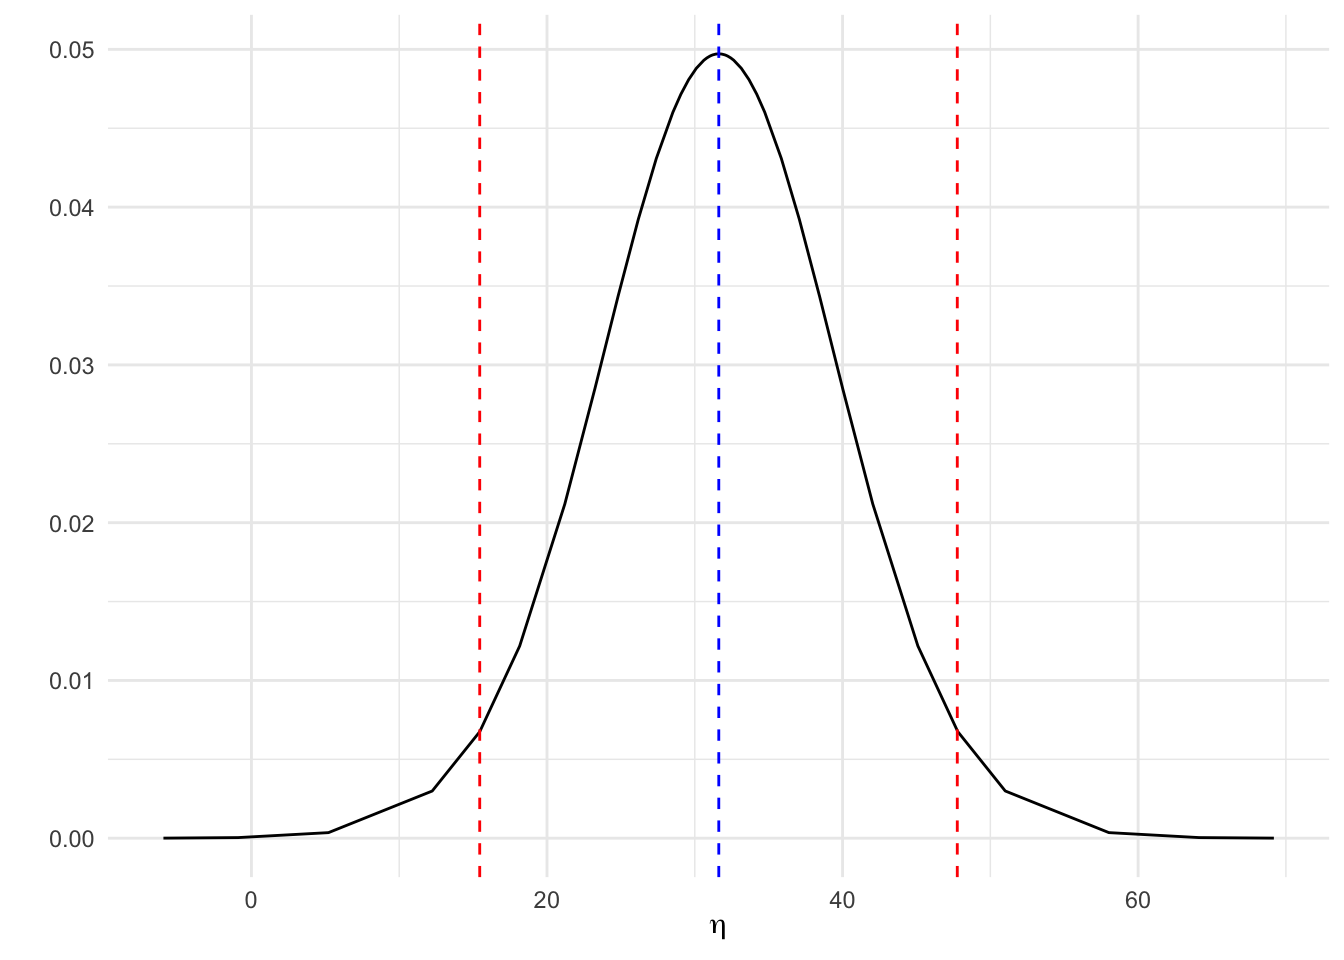
\includegraphics{01-regresion_files/figure-latex/regmul03-1.pdf}
\caption{\label{fig:regmul03}Distribución predictiva a posteriori de SO2 para una configuración dada de los predictores.}
\end{figure}

\hypertarget{conclusiones}{%
\section{Conclusiones}\label{conclusiones}}

En este tema hemos trabajado con el ajuste con INLA de modelos lineales de regresión, esto es, con efectos fijos. En posteriores temas trabajaremos modelos más sofisticados en los que incluiremos los efectos aleatorios, generalizaremos el modelo lineal y entenderemos el planteamiento de modelos a través de modelos jerárquicos bayesianos.

\hypertarget{anova}{%
\chapter{Modelo de ANOVA}\label{anova}}

\hypertarget{introducciuxf3n-1}{%
\section{Introducción}\label{introducciuxf3n-1}}

El modelo de ANOVA se plantea para comparar poblaciones normales, especialmente cuando son más de dos las poblaciones a comparar. Las poblaciones a comparar se identifican a través de una variable clasificadora (de tipo categórico) que actúa como predictora para estimar respuestas medias supuestamente distintas a comparar.

\hypertarget{el-modelo-de-anova}{%
\section{El modelo de ANOVA}\label{el-modelo-de-anova}}

Consideremos una variable respuesta \(Y\) que se distribuye normal, y que viene afectada por una variable de clasificación \(A\) con \(a\) niveles de respuesta distintos (uno por cada una de las poblaciones a comparar). Supongamos que tenemos \(n_i\) observaciones de la respuesta para cada uno de los niveles de respuesta de la variable clasificadora, \(i=1,...,a\). El modelo de ANOVA se plantea asumiendo que en cada nivel o subpoblación, esperamos un valor distinto para la respuesta,
\[(y_{ij}|\mu_i,\sigma^2) \sim N(\mu_i,\sigma^2)\]
de modo que
\[E(y_{ij}|\mu_i,\sigma^2)=\mu_i; \ Var(y_{ij}|\mu_i,\sigma^2)=\sigma^2, \ \ i=1,...,a; \ j=1,...,n_i\]
La formulación habitual de este modelo se suele dar en términos de un efecto global y común a todas las observaciones, \(\theta\), y un efecto diferencial respecto del primer nivel del factor de clasificación \(A\), \(\alpha_i\), con los que se construye la media (identificada generalmente por \(\mu\)) o predictor lineal (identificada generalmente por \(\eta\)) y que en el modelo lineal coinciden:
\[\mu_{ij}=\eta_{ij}=\theta + \alpha_i\]
donde \(\alpha_i=\mu_i-\mu_1\) y \(\mu_1=\theta\), para \(i\geq 1\), esto es, \(\alpha_1=0\).

Estamos pues asumiendo que todos los \(n_i\) sujetos en el subgrupo de población \(i\) identificado por la variable clasificadora \(A\), comparten una media común \(\mu_i\) y cierta variabilidad \(\sigma^2\). Podríamos asumir varianzas distintas para cada subpoblación, pero por simplicidad consideramos que son iguales.

En la modelización bayesiana es preciso añadir distribuciones a priori para cada uno de los parámetros del modelo: los efectos fijos \(\theta,\alpha_i\), y la varianza \(\sigma^2\) de los datos. Ante ausencia de información, se asumirán las distribuciones difusas habituales en INLA:

\begin{eqnarray*}
(Y_{ij}|\mu_i,\sigma^2) & \sim & N(\mu_i,\sigma^2) \\
&& \mu_i = \theta + \alpha_i, i\geq 1 \\
\theta & \sim & N(0,\infty)\\
\alpha_i & \sim & N(0,1000), i\geq 1\\
\tau=1/\sigma^2 & \sim & Ga(1,0.00005)
\end{eqnarray*}

\hypertarget{anova-de-una-vuxeda}{%
\section{Anova de una vía}\label{anova-de-una-vuxeda}}

Vamos a ilustrar el análisis ANOVA en INLA a través de la base de datos \texttt{coagulation}, en la librería \href{https://cran.r-project.org/web/packages/faraway/faraway.pdf}{\texttt{faraway}}, referidos a un estudio de tiempos de coagulación de la sangre en 24 animales a los que aleatoriamente se les asignó una de entre tres dietas distintas (variable clasificadora \texttt{diet}). Posteriormente, para estudiar el efecto de dichas dietas en la coagulación, se tomaron muestras de los tiempos de coagulación (en la variable \texttt{coag}, que es la respuesta).

\begin{Shaded}
\begin{Highlighting}[]
\FunctionTok{data}\NormalTok{(coagulation, }\AttributeTok{package=}\StringTok{"faraway"}\NormalTok{)}
\FunctionTok{str}\NormalTok{(coagulation)}
\CommentTok{\#\textgreater{} \textquotesingle{}data.frame\textquotesingle{}:    24 obs. of  2 variables:}
\CommentTok{\#\textgreater{}  $ coag: num  62 60 63 59 63 67 71 64 65 66 ...}
\CommentTok{\#\textgreater{}  $ diet: Factor w/ 4 levels "A","B","C","D": 1 1 1 1 2 2 2 2 2 2 ...}
\FunctionTok{ggplot}\NormalTok{(coagulation,}\FunctionTok{aes}\NormalTok{(}\AttributeTok{x=}\NormalTok{diet,}\AttributeTok{y=}\NormalTok{coag))}\SpecialCharTok{+}
  \FunctionTok{geom\_boxplot}\NormalTok{(}\FunctionTok{aes}\NormalTok{(}\AttributeTok{color=}\NormalTok{diet))}\SpecialCharTok{+}
  \FunctionTok{theme}\NormalTok{(}\AttributeTok{legend.position=}\StringTok{"none"}\NormalTok{)}
\end{Highlighting}
\end{Shaded}

\includegraphics{02-anova_files/figure-latex/unnamed-chunk-2-1.pdf}

Estamos planteando un modelo de Anova como el propuesto en la sección anterior, donde \(\alpha_i\) identifica el efecto diferencial sobre la respuesta con la dieta A, para el resto de las dietas B y C. Los parámetros del modelo son, como en regresión, los efectos fijos \((\theta,\alpha_i)\) y la varianza \(\sigma^2\), para los que asumimos las priors difusas que por defecto propone INLA. Ajustamos el modelo y obtenemos las inferencias a posteriori

\begin{Shaded}
\begin{Highlighting}[]
\NormalTok{formula}\OtherTok{=}\NormalTok{coag }\SpecialCharTok{\textasciitilde{}}\NormalTok{ diet}
\NormalTok{fit}\OtherTok{=}\FunctionTok{inla}\NormalTok{(formula,}\AttributeTok{family=}\StringTok{"gaussian"}\NormalTok{,}\AttributeTok{data=}\NormalTok{coagulation,}
         \AttributeTok{control.compute=}\FunctionTok{list}\NormalTok{(}\AttributeTok{config=}\ConstantTok{TRUE}\NormalTok{,}\AttributeTok{return.marginals.predictor=}\ConstantTok{TRUE}\NormalTok{))}
\NormalTok{fijos}\OtherTok{=}\FunctionTok{round}\NormalTok{(fit}\SpecialCharTok{$}\NormalTok{summary.fixed,}\DecValTok{3}\NormalTok{);fijos}
\CommentTok{\#\textgreater{}               mean    sd 0.025quant 0.5quant 0.975quant}
\CommentTok{\#\textgreater{} (Intercept) 61.016 1.172     58.700   61.016     63.337}
\CommentTok{\#\textgreater{} dietB        4.979 1.513      1.983    4.980      7.970}
\CommentTok{\#\textgreater{} dietC        6.977 1.513      3.981    6.978      9.968}
\CommentTok{\#\textgreater{} dietD       {-}0.016 1.435     {-}2.859   {-}0.016      2.822}
\CommentTok{\#\textgreater{}             mode kld}
\CommentTok{\#\textgreater{} (Intercept)   NA   0}
\CommentTok{\#\textgreater{} dietB         NA   0}
\CommentTok{\#\textgreater{} dietC         NA   0}
\CommentTok{\#\textgreater{} dietD         NA   0}
\NormalTok{tau}\OtherTok{=}\FunctionTok{round}\NormalTok{(fit}\SpecialCharTok{$}\NormalTok{summary.hyperpar,}\DecValTok{3}\NormalTok{);tau}
\CommentTok{\#\textgreater{}                                          mean    sd}
\CommentTok{\#\textgreater{} Precision for the Gaussian observations 0.197 0.059}
\CommentTok{\#\textgreater{}                                         0.025quant 0.5quant}
\CommentTok{\#\textgreater{} Precision for the Gaussian observations      0.099    0.191}
\CommentTok{\#\textgreater{}                                         0.975quant mode}
\CommentTok{\#\textgreater{} Precision for the Gaussian observations      0.328   NA}
\NormalTok{medias}\OtherTok{=}\FunctionTok{round}\NormalTok{(fit}\SpecialCharTok{$}\NormalTok{summary.linear.predictor,}\DecValTok{4}\NormalTok{)}
\end{Highlighting}
\end{Shaded}

Atendiendo a los descriptivos de la distribución posterior para los efectos fijos, concluimos:

\begin{itemize}
\tightlist
\item
  El tiempo esperado de coagulación para los animales que han seguido la dieta A es de 61.016(58.7,63.337).
\item
  Los animales que han seguido la dieta B tienen un tiempo de coagulación esperado superior en 4.979 unidades a los de la dieta A, y dicha diferencia es \emph{significativamente distinta de cero} en el contexto bayesiano, dado que su RC no incluye al cero, (1.983,7.97).
\item
  Una conclusión similar se deriva para la dieta C, que da un tiempo de coagulación esperado superior en 6.977 unidades a los de la dieta A, y una RC (3.981,9.968).
\item
  Las diferencias en los tiempos de coagulación de seguir una dieta D frente a la dieta A no son relevantes. De hecho, la diferencia entre ellos es de -0.016 y el intervalo RC contiene al cero, (-2.859,2.822).
\end{itemize}

Pintamos a continuación en la Figura \ref{fig:anova01} la distribución posterior de los tiempos esperados de coagulación \(\mu_i\) (o predictores lineales) para cada una de las dietas. En la Figura \ref{fig:anova02} se añaden las medias posteriores y las regiones creíbles.

\begin{Shaded}
\begin{Highlighting}[]
\NormalTok{dietas}\OtherTok{=}\FunctionTok{levels}\NormalTok{(coagulation}\SpecialCharTok{$}\NormalTok{diet)}
\NormalTok{pred}\OtherTok{=}\ConstantTok{NULL}
\ControlFlowTok{for}\NormalTok{(i }\ControlFlowTok{in} \DecValTok{1}\SpecialCharTok{:}\FunctionTok{length}\NormalTok{(dietas))\{}
\NormalTok{index}\OtherTok{=}\FunctionTok{which}\NormalTok{(coagulation}\SpecialCharTok{$}\NormalTok{diet}\SpecialCharTok{==}\NormalTok{dietas[i])[}\DecValTok{1}\NormalTok{]}
\CommentTok{\# distrib. posterior}
\NormalTok{post}\OtherTok{=}\FunctionTok{as.data.frame}\NormalTok{(fit}\SpecialCharTok{$}\NormalTok{marginals.fitted.values[[index]])}
\CommentTok{\# media}
\NormalTok{e}\OtherTok{=}\NormalTok{fit}\SpecialCharTok{$}\NormalTok{summary.fitted.values[index,}\DecValTok{1}\NormalTok{]}
\NormalTok{rc.low}\OtherTok{=}\NormalTok{fit}\SpecialCharTok{$}\NormalTok{summary.fitted.values[index,}\DecValTok{3}\NormalTok{]}
\NormalTok{rc.up}\OtherTok{=}\NormalTok{fit}\SpecialCharTok{$}\NormalTok{summary.fitted.values[index,}\DecValTok{5}\NormalTok{]}
\NormalTok{pred}\OtherTok{=}\FunctionTok{rbind}\NormalTok{(pred,}\FunctionTok{data.frame}\NormalTok{(}\AttributeTok{dieta=}\NormalTok{dietas[i],}
\NormalTok{                           post,e,rc.low,rc.up))}
\NormalTok{\}}

\FunctionTok{ggplot}\NormalTok{(pred, }\FunctionTok{aes}\NormalTok{(}\AttributeTok{x =}\NormalTok{ x, }\AttributeTok{y =}\NormalTok{y)) }\SpecialCharTok{+} 
  \FunctionTok{geom\_line}\NormalTok{(}\FunctionTok{aes}\NormalTok{(}\AttributeTok{color=}\NormalTok{dieta))}\SpecialCharTok{+}
  \FunctionTok{labs}\NormalTok{(}\AttributeTok{x=}\FunctionTok{expression}\NormalTok{(}\FunctionTok{paste}\NormalTok{(}\StringTok{"Tiempo medio de coagulación:"}\NormalTok{,mu)),}
       \AttributeTok{y=}\StringTok{"D.Posterior"}\NormalTok{)}
\end{Highlighting}
\end{Shaded}

\begin{figure}
\centering
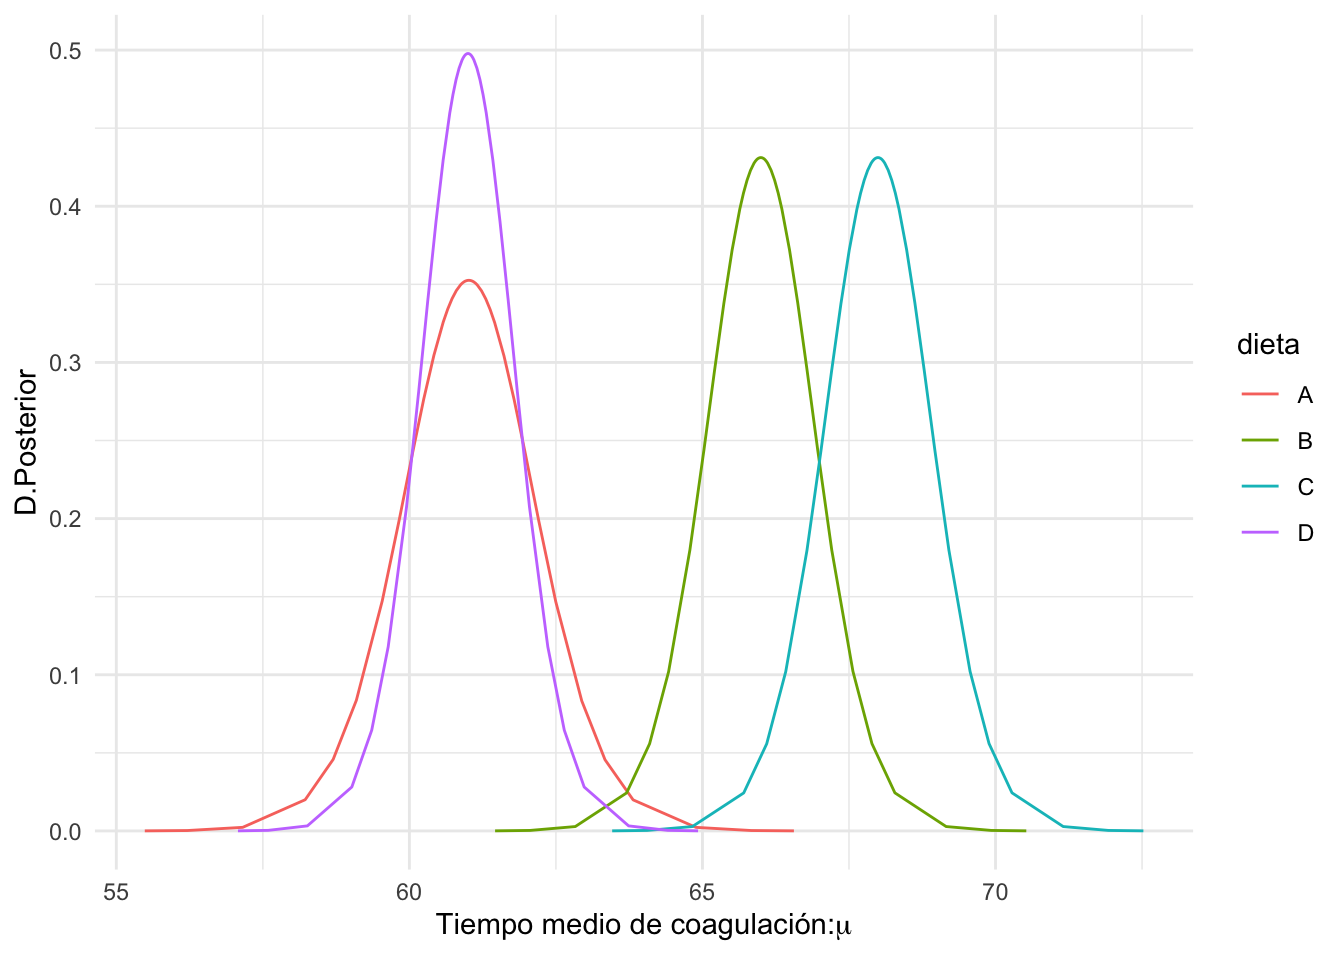
\includegraphics{02-anova_files/figure-latex/anova01-1.pdf}
\caption{\label{fig:anova01}Distribución posterior del tiempo medio de coagulación para las 4 dietas.}
\end{figure}

Podríamos ajustar el modelo prescindiendo del efecto de interceptación y estimar directamente los efectos.

\begin{Shaded}
\begin{Highlighting}[]
\NormalTok{formula}\OtherTok{=}\NormalTok{coag }\SpecialCharTok{\textasciitilde{}} \SpecialCharTok{{-}}\DecValTok{1} \SpecialCharTok{+}\NormalTok{ diet}
\NormalTok{fit}\OtherTok{=}\FunctionTok{inla}\NormalTok{(formula,}\AttributeTok{family=}\StringTok{"gaussian"}\NormalTok{,}\AttributeTok{data=}\NormalTok{coagulation,}
         \AttributeTok{control.compute=}\FunctionTok{list}\NormalTok{(}\AttributeTok{config=}\ConstantTok{TRUE}\NormalTok{,}\AttributeTok{return.marginals.predictor=}\ConstantTok{TRUE}\NormalTok{))}
\FunctionTok{round}\NormalTok{(fit}\SpecialCharTok{$}\NormalTok{summary.fixed,}\DecValTok{3}\NormalTok{)}
\CommentTok{\#\textgreater{}         mean    sd 0.025quant 0.5quant 0.975quant mode kld}
\CommentTok{\#\textgreater{} dietA 60.916 1.176     58.577   60.919     63.233   NA   0}
\CommentTok{\#\textgreater{} dietB 65.939 0.961     64.030   65.942     67.832   NA   0}
\CommentTok{\#\textgreater{} dietC 67.937 0.961     66.028   67.940     69.830   NA   0}
\CommentTok{\#\textgreater{} dietD 60.958 0.832     59.306   60.960     62.599   NA   0}
\FunctionTok{round}\NormalTok{(fit}\SpecialCharTok{$}\NormalTok{summary.hyperpar,}\DecValTok{3}\NormalTok{)}
\CommentTok{\#\textgreater{}                                          mean   sd}
\CommentTok{\#\textgreater{} Precision for the Gaussian observations 0.197 0.06}
\CommentTok{\#\textgreater{}                                         0.025quant 0.5quant}
\CommentTok{\#\textgreater{} Precision for the Gaussian observations      0.098     0.19}
\CommentTok{\#\textgreater{}                                         0.975quant mode}
\CommentTok{\#\textgreater{} Precision for the Gaussian observations      0.324   NA}
\end{Highlighting}
\end{Shaded}

Con lo cual la representación gráfica se simplifica a través, directamente, de las distrubuciones posteriores de los efectos fijos.

\begin{Shaded}
\begin{Highlighting}[]
\NormalTok{pred}\OtherTok{=}\ConstantTok{NULL}
\ControlFlowTok{for}\NormalTok{(i }\ControlFlowTok{in} \DecValTok{1}\SpecialCharTok{:}\FunctionTok{length}\NormalTok{(}\FunctionTok{names}\NormalTok{(fit}\SpecialCharTok{$}\NormalTok{marginals.fixed)))\{}
\NormalTok{  pred}\OtherTok{=}\FunctionTok{rbind}\NormalTok{(pred,}\FunctionTok{data.frame}\NormalTok{(}\FunctionTok{as.data.frame}\NormalTok{(fit}\SpecialCharTok{$}\NormalTok{marginals.fixed[[i]]),}
                  \AttributeTok{dieta=}\FunctionTok{names}\NormalTok{(fit}\SpecialCharTok{$}\NormalTok{marginals.fixed)[i],}
                  \AttributeTok{mean=}\NormalTok{fit}\SpecialCharTok{$}\NormalTok{summary.fixed}\SpecialCharTok{$}\NormalTok{mean[i],}
                  \AttributeTok{rc.low=}\NormalTok{fit}\SpecialCharTok{$}\NormalTok{summary.fixed}\SpecialCharTok{$}\StringTok{\textquotesingle{}0.025quant\textquotesingle{}}\NormalTok{[i],}
                  \AttributeTok{rc.up=}\NormalTok{fit}\SpecialCharTok{$}\NormalTok{summary.fixed}\SpecialCharTok{$}\StringTok{\textquotesingle{}0.975quant\textquotesingle{}}\NormalTok{[i]))\}}

\FunctionTok{ggplot}\NormalTok{(pred, }\FunctionTok{aes}\NormalTok{(}\AttributeTok{x =}\NormalTok{ x, }\AttributeTok{y =}\NormalTok{y)) }\SpecialCharTok{+} 
  \FunctionTok{geom\_line}\NormalTok{(}\FunctionTok{aes}\NormalTok{(}\AttributeTok{color=}\NormalTok{dieta))}\SpecialCharTok{+}
  \FunctionTok{geom\_vline}\NormalTok{(}\FunctionTok{aes}\NormalTok{(}\AttributeTok{xintercept=}\NormalTok{mean,}\AttributeTok{color=}\NormalTok{dieta),}\AttributeTok{linetype=}\StringTok{"dashed"}\NormalTok{)}\SpecialCharTok{+}
  \FunctionTok{geom\_vline}\NormalTok{(}\FunctionTok{aes}\NormalTok{(}\AttributeTok{xintercept=}\NormalTok{rc.low,}\AttributeTok{color=}\NormalTok{dieta),}\AttributeTok{linetype=}\StringTok{"dotted"}\NormalTok{)}\SpecialCharTok{+}
  \FunctionTok{geom\_vline}\NormalTok{(}\FunctionTok{aes}\NormalTok{(}\AttributeTok{xintercept=}\NormalTok{rc.up,}\AttributeTok{color=}\NormalTok{dieta),}\AttributeTok{linetype=}\StringTok{"dotted"}\NormalTok{)}\SpecialCharTok{+}
  \FunctionTok{facet\_wrap}\NormalTok{(}\FunctionTok{vars}\NormalTok{(dieta))}\SpecialCharTok{+}
  \FunctionTok{labs}\NormalTok{(}\AttributeTok{x=}\FunctionTok{expression}\NormalTok{(}\FunctionTok{paste}\NormalTok{(}\StringTok{"Tiempo medio de coagulación:"}\NormalTok{,mu)),}
       \AttributeTok{y=}\StringTok{"D.Posterior"}\NormalTok{,}\AttributeTok{title=}\StringTok{"D.Posterior, medias y RC95\%"}\NormalTok{)}\SpecialCharTok{+}
  \FunctionTok{theme}\NormalTok{(}\AttributeTok{legend.position=}\StringTok{"none"}\NormalTok{)}
\end{Highlighting}
\end{Shaded}

\begin{figure}
\centering
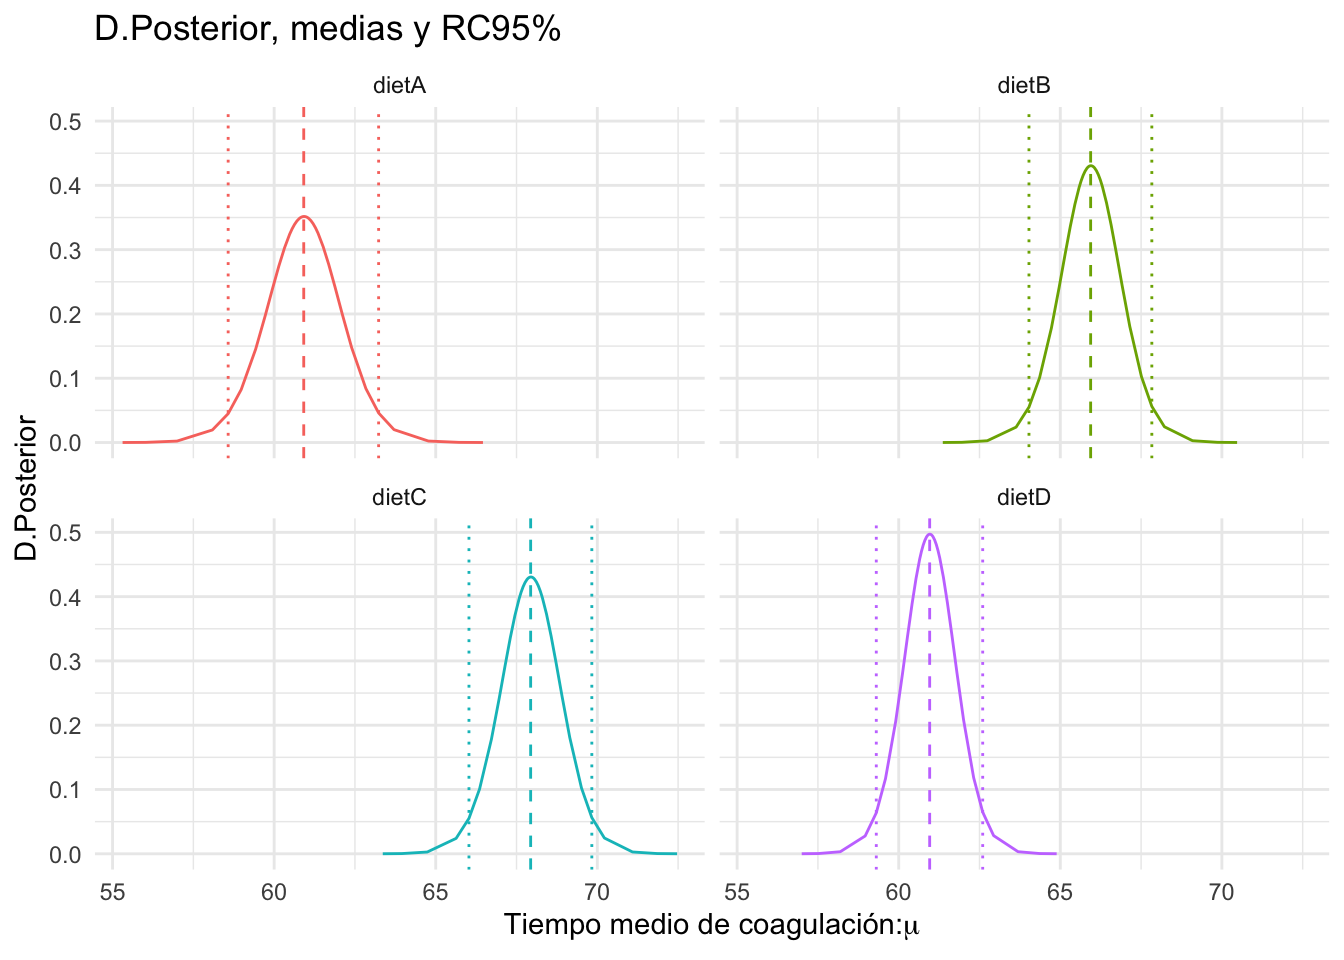
\includegraphics{02-anova_files/figure-latex/anova02-1.pdf}
\caption{\label{fig:anova02}Distribuciones posteriores, medias y RC del tiempo esperado de coagulación.}
\end{figure}

Como ya hacíamos en regresión, podemos inferir sobre la desviación típica de los datos, \(\sigma\), transformando la distribución para la precisión \(\tau\). La distribución posterior junto con su media y RC95\% se muestra en la Figura \ref{fig:anova03}.

\begin{Shaded}
\begin{Highlighting}[]
\NormalTok{sigma.post}\OtherTok{=}\FunctionTok{inla.tmarginal}\NormalTok{(}\ControlFlowTok{function}\NormalTok{(tau) tau}\SpecialCharTok{\^{}}\NormalTok{(}\SpecialCharTok{{-}}\DecValTok{1}\SpecialCharTok{/}\DecValTok{2}\NormalTok{),}
\NormalTok{  fit}\SpecialCharTok{$}\NormalTok{marginals.hyperpar[[}\DecValTok{1}\NormalTok{]])}
\CommentTok{\# y la pintamos}
\FunctionTok{ggplot}\NormalTok{(}\FunctionTok{as.data.frame}\NormalTok{(sigma.post)) }\SpecialCharTok{+} 
  \FunctionTok{geom\_line}\NormalTok{(}\FunctionTok{aes}\NormalTok{(}\AttributeTok{x =}\NormalTok{ x, }\AttributeTok{y =}\NormalTok{ y)) }\SpecialCharTok{+}
  \FunctionTok{labs}\NormalTok{(}\AttributeTok{x=}\FunctionTok{expression}\NormalTok{(sigma),}\AttributeTok{y=}\StringTok{"D.Posterior"}\NormalTok{)}\SpecialCharTok{+}
  \FunctionTok{geom\_vline}\NormalTok{(}\AttributeTok{xintercept=}\FunctionTok{inla.hpdmarginal}\NormalTok{(}\FloatTok{0.95}\NormalTok{,sigma.post),}
             \AttributeTok{linetype=}\StringTok{"dotted"}\NormalTok{,}\AttributeTok{color=}\StringTok{"blue"}\NormalTok{)}\SpecialCharTok{+}
  \FunctionTok{geom\_vline}\NormalTok{(}\AttributeTok{xintercept=}\FunctionTok{inla.emarginal}\NormalTok{(}\ControlFlowTok{function}\NormalTok{(x) x,sigma.post),}
             \AttributeTok{linetype=}\StringTok{"dashed"}\NormalTok{,}\AttributeTok{color=}\StringTok{"blue"}\NormalTok{)}
\end{Highlighting}
\end{Shaded}

\begin{figure}
\centering
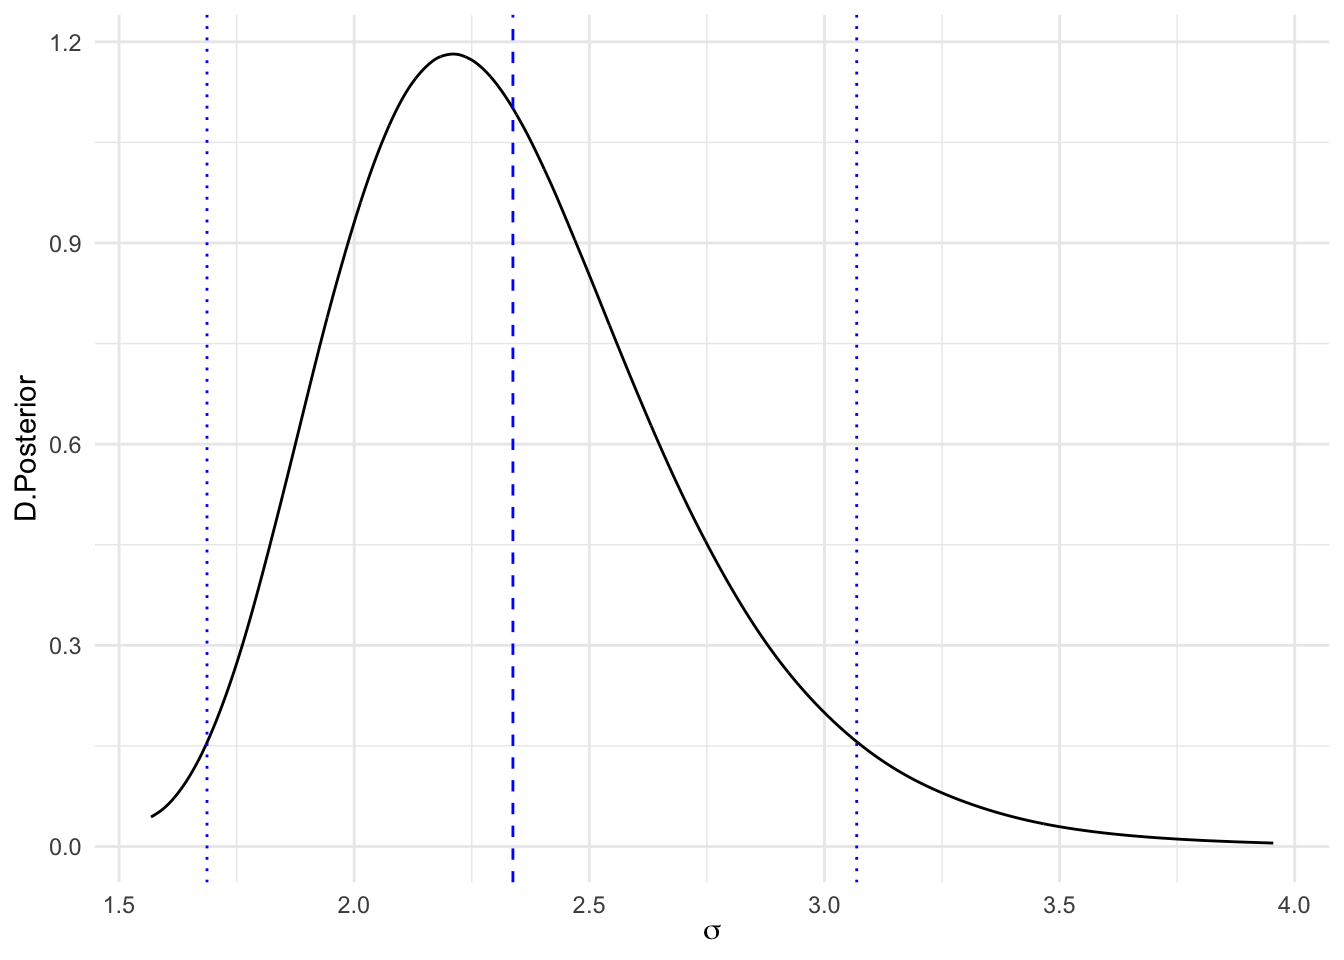
\includegraphics{02-anova_files/figure-latex/anova03-1.pdf}
\caption{\label{fig:anova03}Distribución posterior, media y RC, de la desviación típica de los datos (sigma)}
\end{figure}

\begin{Shaded}
\begin{Highlighting}[]

\CommentTok{\# Valor esperado}
\NormalTok{sigma.e}\OtherTok{=}\FunctionTok{round}\NormalTok{(}\FunctionTok{inla.emarginal}\NormalTok{(}\ControlFlowTok{function}\NormalTok{(tau) tau}\SpecialCharTok{\^{}}\NormalTok{(}\SpecialCharTok{{-}}\DecValTok{1}\SpecialCharTok{/}\DecValTok{2}\NormalTok{),}
\NormalTok{  fit}\SpecialCharTok{$}\NormalTok{marginals.hyperpar[[}\DecValTok{1}\NormalTok{]]),}\DecValTok{4}\NormalTok{)}
\CommentTok{\# HPD95\%}
\NormalTok{sigma.hpd}\OtherTok{=}\FunctionTok{round}\NormalTok{(}\FunctionTok{inla.hpdmarginal}\NormalTok{(}\FloatTok{0.95}\NormalTok{,sigma.post),}\DecValTok{3}\NormalTok{)}
\FunctionTok{paste}\NormalTok{(}\StringTok{"E(sigma.post)="}\NormalTok{,sigma.e,}\StringTok{"HPD95\%=("}\NormalTok{,sigma.hpd[}\DecValTok{1}\NormalTok{],}\StringTok{","}\NormalTok{,sigma.hpd[}\DecValTok{2}\NormalTok{],}\StringTok{")"}\NormalTok{)}
\CommentTok{\#\textgreater{} [1] "E(sigma.post)= 2.3379 HPD95\%=( 1.687 , 3.069 )"}
\end{Highlighting}
\end{Shaded}

Si queremos inferir sobre la diferencia entre cualesquiera de los efectos podemos recurrir a simular la distribución posterior de las diferencias. Por ejemplo, supongamos que queremos comparar la dieta B con la dieta D. Simulamos entonces de las distribuciones posteriores de \(\mu_B\) y de \(\mu_D\), y obtenemos la diferencia \(\mu_B-\mu_D\).

\begin{Shaded}
\begin{Highlighting}[]
\NormalTok{sims}\OtherTok{=}\FunctionTok{inla.posterior.sample}\NormalTok{(}\DecValTok{1000}\NormalTok{,fit,}\AttributeTok{selection=}\FunctionTok{list}\NormalTok{(}\AttributeTok{dietB=}\DecValTok{1}\NormalTok{,}\AttributeTok{dietD=}\DecValTok{1}\NormalTok{))}
\NormalTok{dif\_BD}\OtherTok{=}\FunctionTok{as.vector}\NormalTok{(}\FunctionTok{inla.posterior.sample.eval}\NormalTok{(}\ControlFlowTok{function}\NormalTok{(...) dietB}\SpecialCharTok{{-}}\NormalTok{dietD, sims))}
\NormalTok{pred}\OtherTok{=}\FunctionTok{data.frame}\NormalTok{(}\AttributeTok{dif=}\NormalTok{dif\_BD)}
\FunctionTok{ggplot}\NormalTok{(pred,}\FunctionTok{aes}\NormalTok{(}\AttributeTok{x=}\NormalTok{dif))}\SpecialCharTok{+}
  \FunctionTok{geom\_histogram}\NormalTok{(}\FunctionTok{aes}\NormalTok{(}\AttributeTok{y=}\NormalTok{..density..), }\AttributeTok{colour=}\StringTok{"black"}\NormalTok{, }\AttributeTok{fill=}\StringTok{"white"}\NormalTok{)}\SpecialCharTok{+}
 \FunctionTok{geom\_density}\NormalTok{(}\AttributeTok{alpha=}\NormalTok{.}\DecValTok{2}\NormalTok{, }\AttributeTok{fill=}\StringTok{"\#80E7F5"}\NormalTok{)}\SpecialCharTok{+}
  \FunctionTok{geom\_vline}\NormalTok{(}\AttributeTok{xintercept=}\FunctionTok{mean}\NormalTok{(dif\_BD),}\AttributeTok{color=}\StringTok{"red"}\NormalTok{,}\AttributeTok{size=}\FloatTok{1.5}\NormalTok{)}\SpecialCharTok{+}
  \FunctionTok{geom\_vline}\NormalTok{(}\AttributeTok{xintercept=}\FunctionTok{quantile}\NormalTok{(dif\_BD,}\AttributeTok{probs=}\FunctionTok{c}\NormalTok{(}\FloatTok{0.025}\NormalTok{,}\FloatTok{0.975}\NormalTok{)),}\AttributeTok{color=}\StringTok{"red"}\NormalTok{,}\AttributeTok{size=}\FloatTok{1.5}\NormalTok{,}\AttributeTok{linetype=}\StringTok{"dashed"}\NormalTok{)}\SpecialCharTok{+}
  \FunctionTok{labs}\NormalTok{(}\AttributeTok{x=}\StringTok{"Diferencia del tiempo esperado de coagulación: dietB{-}dietD"}\NormalTok{,}\AttributeTok{y=}\StringTok{""}\NormalTok{)}
\CommentTok{\#\textgreater{} \textasciigrave{}stat\_bin()\textasciigrave{} using \textasciigrave{}bins = 30\textasciigrave{}. Pick better value with}
\CommentTok{\#\textgreater{} \textasciigrave{}binwidth\textasciigrave{}.}
\end{Highlighting}
\end{Shaded}

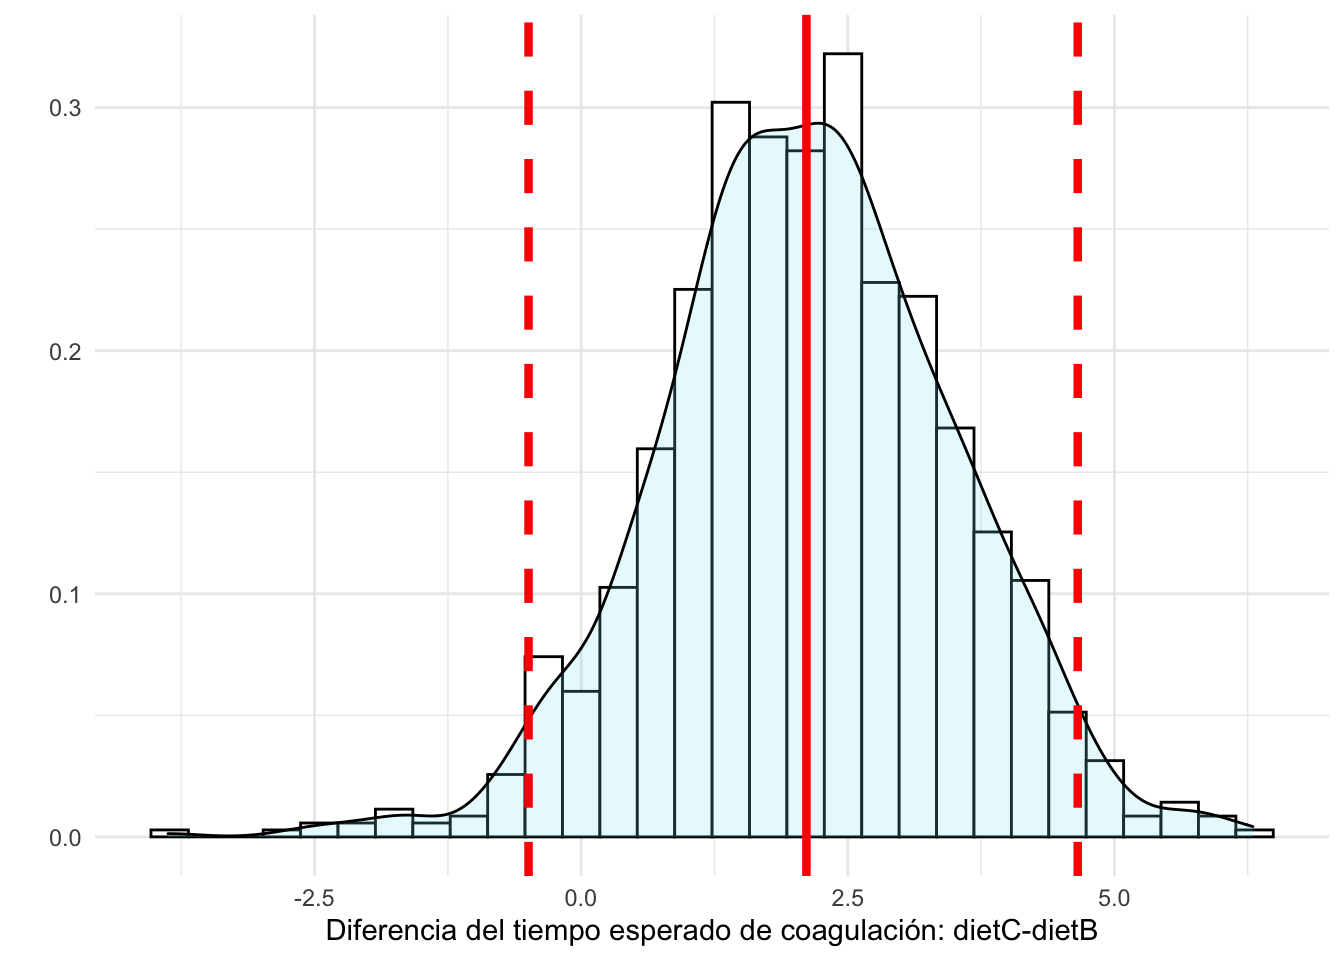
\includegraphics{02-anova_files/figure-latex/unnamed-chunk-5-1.pdf}

\hypertarget{anova-de-varias-vuxedas}{%
\section{Anova de varias vías}\label{anova-de-varias-vuxedas}}

Generalmente, y en especial cuando trabajamos con experimentación, son varios los factores que controlamos para investigar el efecto que producen en una respuesta continua. Hablamos de modelos de Anova de varias vías.

Utilizamos la base de datos \texttt{butterfat} en la librería \href{https://cran.r-project.org/web/packages/faraway/faraway.pdf}{\texttt{faraway}} para ilustrar el ajuste con INLA de un modelo de Anova de varias vías. Esta base de datos contiene 100 registros del contenido en grasa láctea, \texttt{Butterfat}, para muestras aleatorias de 20 vacas (10 de ellas de 2 años y 10 maduras, con más de 4 años -en la variable \texttt{Age}) de cada una de cinco razas (en la variable \texttt{Breed}).

El objetivo es investigar las diferencias en materia grasa entre razas y edad, con el fin último de identificar cuáles producen más materia grasa y cuáles menos. Veamos los datos en la Figura \ref{fig:butterfat1}.

\begin{Shaded}
\begin{Highlighting}[]
\FunctionTok{data}\NormalTok{(butterfat,}\AttributeTok{package=}\StringTok{"faraway"}\NormalTok{)}
\FunctionTok{str}\NormalTok{(butterfat)}
\CommentTok{\#\textgreater{} \textquotesingle{}data.frame\textquotesingle{}:    100 obs. of  3 variables:}
\CommentTok{\#\textgreater{}  $ Butterfat: num  3.74 4.01 3.77 3.78 4.1 4.06 4.27 3.94 4.11 4.25 ...}
\CommentTok{\#\textgreater{}  $ Breed    : Factor w/ 5 levels "Ayrshire","Canadian",..: 1 1 1 1 1 1 1 1 1 1 ...}
\CommentTok{\#\textgreater{}  $ Age      : Factor w/ 2 levels "2year","Mature": 2 1 2 1 2 1 2 1 2 1 ...}
\FunctionTok{ggplot}\NormalTok{(butterfat,}\FunctionTok{aes}\NormalTok{(}\AttributeTok{x=}\NormalTok{Breed,}\AttributeTok{y=}\NormalTok{Butterfat))}\SpecialCharTok{+}
  \FunctionTok{geom\_boxplot}\NormalTok{(}\FunctionTok{aes}\NormalTok{(}\AttributeTok{color=}\NormalTok{Age))}\SpecialCharTok{+}
  \FunctionTok{coord\_flip}\NormalTok{()}
\end{Highlighting}
\end{Shaded}

\begin{figure}
\centering
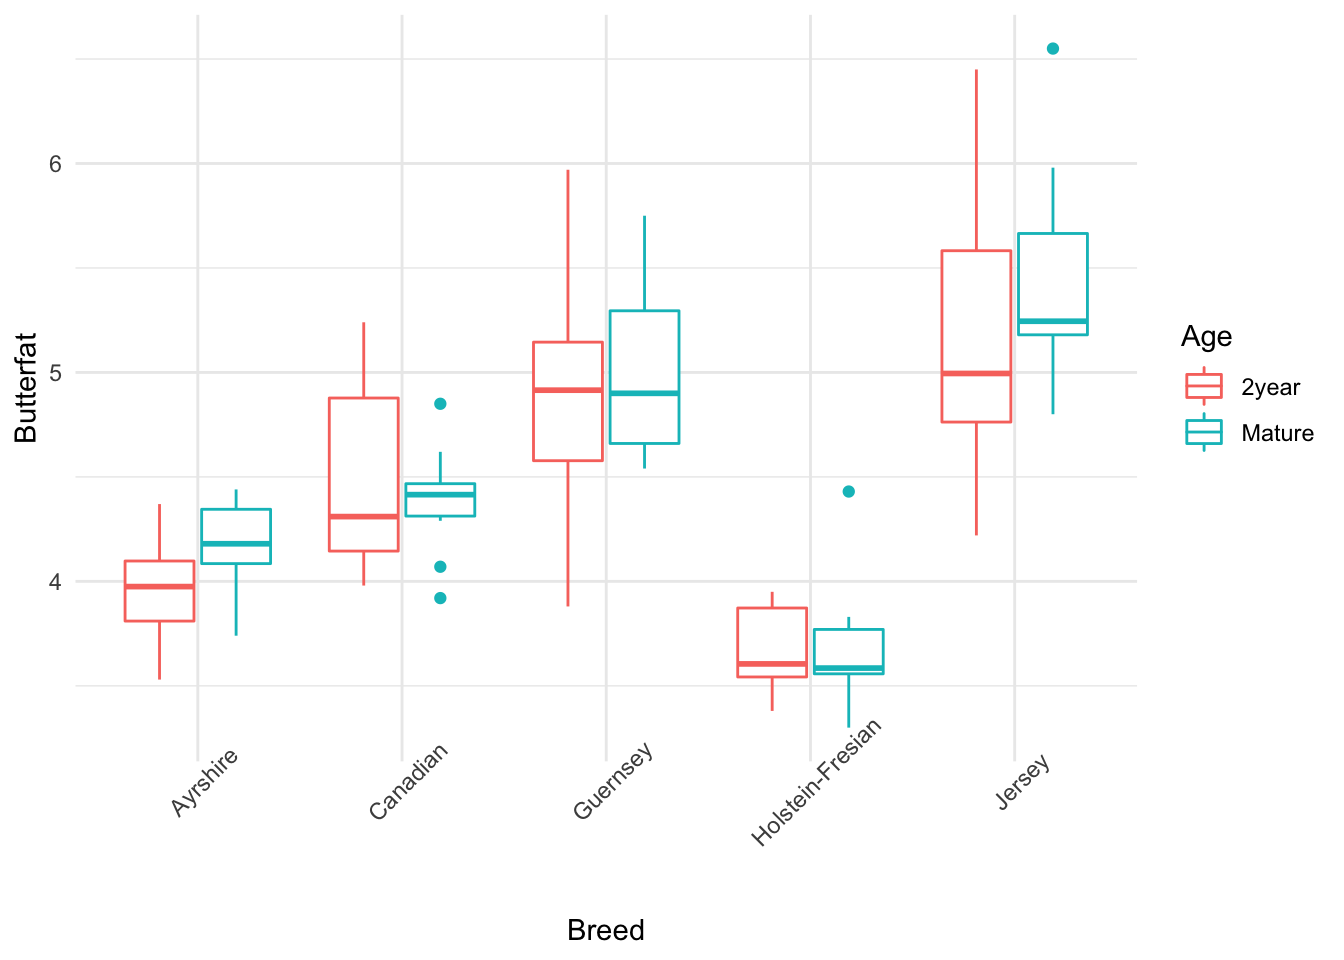
\includegraphics{02-anova_files/figure-latex/butterfat1-1.pdf}
\caption{\label{fig:butterfat1}Base de datos butterfat, en la librería Faraway}
\end{figure}

A la vista del gráfico, apreciamos que por lo general, en la mayoría de las razas, las vacas más jóvenes tienen menor contenido en materia grasa que las más viejas. Sin embargo, tal afirmación no parece tan clara en las razas \emph{Guernsey} y \emph{Holstein-Fresian}, de modo que para modelizar nuestros datos vamos a considerar a priori, la posibilidad de interacciones entre los factores de clasificación \texttt{Breed} y \texttt{Age}.

Cuando nos enfrentamos a varios factores de clasificación, cabe la posibilidad de que interaccionen entre ellos, esto es, que en algunos niveles de un factor actúen de forma diferente a los otros cuando se combinan con los niveles de algún otro factor. El orden de una interacción viene dado por el número de factores de clasificación que involucra, de modo que hablamos de interacciones de orden 2 si consideramos la interacción entre dos factores, de orden 3 si consideramos la interacción entre tres factores, etc. Generalmente trabajamos con interacciones de orden bajo, dada la complejidad de las conclusiones en interacciones de orden alto. Por otro lado, siempre es importante tener en cuenta de cuántos datos disponemos para conocer a priori la posibilidad de estimar con fiabilidad los distintos efectos de interacción: una interacción de dos factores con \(n_1\) y \(n_2\) niveles de clasificación respectivamente, revierte en la estimación de \((n_1-1)\times(n_2-1)\) efectos de interacción adicionales.

Así, en nuestro problema si estamos planteando la posibilidad de que haya interacciones entre los dos factores de clasificación, estamos asumiendo un modelo de tipo siguiente, asumiendo normalidad en la respuesta:

\[(y_{ijk}|\mu_{ij},\sigma^2) \sim N(\mu_{ij},\sigma^2)\]
con
\[\mu_{ij}=\theta+ \alpha_i + \beta_j + \alpha\beta_{ij}\]
donde en nuestro ejemplo, \(\alpha_i\) es el efecto diferencial (respecto del primer nivel) que aporta el nivel \(i\) de la variable \texttt{Breed}, \(\beta_j\) el efecto asociado a la variable \texttt{Age}, y \(\alpha\beta\) la correspondiente interacción entre ellas. En \emph{R} una interacción de orden 2 entre dos variables \(f_1\) y \(f_2\) se especifica con \(f_1:f_2\); los efectos principales y la interacción se pueden especificar de varios modos alternativos:
\[f_1+f_2+f_1:f_2 \equiv f_1*f_2 \equiv (f_1+f_2)\^2\]

Veamos cómo ajustar con INLA este modelo, recabando también los criterios de selección DIC y WAIC.

\begin{Shaded}
\begin{Highlighting}[]
\NormalTok{formula}\OtherTok{=}\NormalTok{Butterfat }\SpecialCharTok{\textasciitilde{}}\NormalTok{ Breed }\SpecialCharTok{*}\NormalTok{ Age}
\NormalTok{fit}\OtherTok{=}\FunctionTok{inla}\NormalTok{(formula,}\AttributeTok{data=}\NormalTok{butterfat,}
         \AttributeTok{control.compute=}\FunctionTok{list}\NormalTok{(}\AttributeTok{dic =} \ConstantTok{TRUE}\NormalTok{, }\AttributeTok{waic =} \ConstantTok{TRUE}\NormalTok{))}
\FunctionTok{round}\NormalTok{(fit}\SpecialCharTok{$}\NormalTok{summary.fixed,}\DecValTok{3}\NormalTok{)}
\CommentTok{\#\textgreater{}                                   mean    sd 0.025quant}
\CommentTok{\#\textgreater{} (Intercept)                      3.966 0.131      3.708}
\CommentTok{\#\textgreater{} BreedCanadian                    0.522 0.186      0.157}
\CommentTok{\#\textgreater{} BreedGuernsey                    0.933 0.186      0.568}
\CommentTok{\#\textgreater{} BreedHolstein{-}Fresian           {-}0.303 0.186     {-}0.668}
\CommentTok{\#\textgreater{} BreedJersey                      1.167 0.186      0.802}
\CommentTok{\#\textgreater{} AgeMature                        0.188 0.186     {-}0.177}
\CommentTok{\#\textgreater{} BreedCanadian:AgeMature         {-}0.287 0.263     {-}0.804}
\CommentTok{\#\textgreater{} BreedGuernsey:AgeMature         {-}0.086 0.263     {-}0.603}
\CommentTok{\#\textgreater{} BreedHolstein{-}Fresian:AgeMature {-}0.175 0.263     {-}0.692}
\CommentTok{\#\textgreater{} BreedJersey:AgeMature            0.131 0.263     {-}0.386}
\CommentTok{\#\textgreater{}                                 0.5quant 0.975quant mode}
\CommentTok{\#\textgreater{} (Intercept)                        3.966      4.224   NA}
\CommentTok{\#\textgreater{} BreedCanadian                      0.522      0.887   NA}
\CommentTok{\#\textgreater{} BreedGuernsey                      0.933      1.298   NA}
\CommentTok{\#\textgreater{} BreedHolstein{-}Fresian             {-}0.303      0.062   NA}
\CommentTok{\#\textgreater{} BreedJersey                        1.167      1.532   NA}
\CommentTok{\#\textgreater{} AgeMature                          0.188      0.553   NA}
\CommentTok{\#\textgreater{} BreedCanadian:AgeMature           {-}0.287      0.230   NA}
\CommentTok{\#\textgreater{} BreedGuernsey:AgeMature           {-}0.086      0.431   NA}
\CommentTok{\#\textgreater{} BreedHolstein{-}Fresian:AgeMature   {-}0.175      0.342   NA}
\CommentTok{\#\textgreater{} BreedJersey:AgeMature              0.131      0.648   NA}
\CommentTok{\#\textgreater{}                                 kld}
\CommentTok{\#\textgreater{} (Intercept)                       0}
\CommentTok{\#\textgreater{} BreedCanadian                     0}
\CommentTok{\#\textgreater{} BreedGuernsey                     0}
\CommentTok{\#\textgreater{} BreedHolstein{-}Fresian             0}
\CommentTok{\#\textgreater{} BreedJersey                       0}
\CommentTok{\#\textgreater{} AgeMature                         0}
\CommentTok{\#\textgreater{} BreedCanadian:AgeMature           0}
\CommentTok{\#\textgreater{} BreedGuernsey:AgeMature           0}
\CommentTok{\#\textgreater{} BreedHolstein{-}Fresian:AgeMature   0}
\CommentTok{\#\textgreater{} BreedJersey:AgeMature             0}
\NormalTok{fit}\SpecialCharTok{$}\NormalTok{dic}\SpecialCharTok{$}\NormalTok{dic}
\CommentTok{\#\textgreater{} [1] 120.4908}
\NormalTok{fit}\SpecialCharTok{$}\NormalTok{waic}\SpecialCharTok{$}\NormalTok{waic}
\CommentTok{\#\textgreater{} [1] 121.7376}
\end{Highlighting}
\end{Shaded}

Observamos en la inferencia posterior para los efectos fijos, que todas las RC asociadas a los efectos de interacción contienen al cero, lo que descarta la relevancia de la interacción a la hora de predecir la respuesta. Reajustamos pues el modelo eliminando la interacción, y comprobamos que efectivamente al eliminarla conseguimos reducir los valores del DIC y WAIC que usamos habitualmente para la selección de variables.

\begin{Shaded}
\begin{Highlighting}[]
\NormalTok{formula}\OtherTok{=}\NormalTok{Butterfat }\SpecialCharTok{\textasciitilde{}}\NormalTok{ Breed }\SpecialCharTok{+}\NormalTok{ Age}
\NormalTok{fit}\OtherTok{=}\FunctionTok{inla}\NormalTok{(formula,}\AttributeTok{data=}\NormalTok{butterfat,}
         \AttributeTok{control.predictor=}\FunctionTok{list}\NormalTok{(}\AttributeTok{compute=}\ConstantTok{TRUE}\NormalTok{),}
         \AttributeTok{control.compute=}\FunctionTok{list}\NormalTok{(}\AttributeTok{return.marginals.predictor=}\ConstantTok{TRUE}\NormalTok{,}
                              \AttributeTok{dic =} \ConstantTok{TRUE}\NormalTok{, }\AttributeTok{waic =} \ConstantTok{TRUE}\NormalTok{))}
\NormalTok{fit}\SpecialCharTok{$}\NormalTok{summary.fixed}
\CommentTok{\#\textgreater{}                             mean         sd  0.025quant}
\CommentTok{\#\textgreater{} (Intercept)            4.0077184 0.10124860  3.80873701}
\CommentTok{\#\textgreater{} BreedCanadian          0.3784787 0.13071136  0.12159362}
\CommentTok{\#\textgreater{} BreedGuernsey          0.8899744 0.13071136  0.63308913}
\CommentTok{\#\textgreater{} BreedHolstein{-}Fresian {-}0.3905147 0.13071136 {-}0.64739962}
\CommentTok{\#\textgreater{} BreedJersey            1.2324714 0.13071136  0.97558612}
\CommentTok{\#\textgreater{} AgeMature              0.1045993 0.08267009 {-}0.05787069}
\CommentTok{\#\textgreater{}                         0.5quant 0.975quant mode}
\CommentTok{\#\textgreater{} (Intercept)            4.0077182  4.2067008   NA}
\CommentTok{\#\textgreater{} BreedCanadian          0.3784790  0.6353626   NA}
\CommentTok{\#\textgreater{} BreedGuernsey          0.8899746  1.1468581   NA}
\CommentTok{\#\textgreater{} BreedHolstein{-}Fresian {-}0.3905145 {-}0.1336306   NA}
\CommentTok{\#\textgreater{} BreedJersey            1.2324717  1.4893551   NA}
\CommentTok{\#\textgreater{} AgeMature              0.1045993  0.2670692   NA}
\CommentTok{\#\textgreater{}                                kld}
\CommentTok{\#\textgreater{} (Intercept)           2.525012e{-}09}
\CommentTok{\#\textgreater{} BreedCanadian         2.524990e{-}09}
\CommentTok{\#\textgreater{} BreedGuernsey         2.524990e{-}09}
\CommentTok{\#\textgreater{} BreedHolstein{-}Fresian 2.524988e{-}09}
\CommentTok{\#\textgreater{} BreedJersey           2.524990e{-}09}
\CommentTok{\#\textgreater{} AgeMature             2.525221e{-}09}
\NormalTok{fit}\SpecialCharTok{$}\NormalTok{waic}\SpecialCharTok{$}\NormalTok{waic}
\CommentTok{\#\textgreater{} [1] 116.3439}
\NormalTok{fit}\SpecialCharTok{$}\NormalTok{dic}\SpecialCharTok{$}\NormalTok{dic}
\CommentTok{\#\textgreater{} [1] 115.3807}
\end{Highlighting}
\end{Shaded}

Observamos ya a partir del modelo ajustado, que el efecto de la edad no es relevante (su RC incluye al cero), pero sin embargo sí que hay diferencias debido a las razas.

Reajustamos de nuevo el modelo, excluyendo la variable \texttt{Age}, y verificamos la reducción (ligera) del DIC/WAIC, lo cual justifica usar este modelo para la predicción.

\begin{Shaded}
\begin{Highlighting}[]
\NormalTok{formula}\OtherTok{=}\NormalTok{Butterfat }\SpecialCharTok{\textasciitilde{}}\NormalTok{ Breed }
\NormalTok{fit}\OtherTok{=}\FunctionTok{inla}\NormalTok{(formula,}\AttributeTok{data=}\NormalTok{butterfat,}
         \AttributeTok{control.predictor=}\FunctionTok{list}\NormalTok{(}\AttributeTok{compute=}\ConstantTok{TRUE}\NormalTok{),}
         \AttributeTok{control.compute=}\FunctionTok{list}\NormalTok{(}\AttributeTok{return.marginals.predictor=}\ConstantTok{TRUE}\NormalTok{,}
                              \AttributeTok{dic =} \ConstantTok{TRUE}\NormalTok{, }\AttributeTok{waic =} \ConstantTok{TRUE}\NormalTok{))}
\NormalTok{fit}\SpecialCharTok{$}\NormalTok{summary.fixed}
\CommentTok{\#\textgreater{}                             mean         sd 0.025quant}
\CommentTok{\#\textgreater{} (Intercept)            4.0600181 0.09271695  3.8778078}
\CommentTok{\#\textgreater{} BreedCanadian          0.3784786 0.13112185  0.1207924}
\CommentTok{\#\textgreater{} BreedGuernsey          0.8899742 0.13112185  0.6322879}
\CommentTok{\#\textgreater{} BreedHolstein{-}Fresian {-}0.3905148 0.13112185 {-}0.6482008}
\CommentTok{\#\textgreater{} BreedJersey            1.2324713 0.13112185  0.9747849}
\CommentTok{\#\textgreater{}                         0.5quant 0.975quant mode}
\CommentTok{\#\textgreater{} (Intercept)            4.0600180  4.2422295   NA}
\CommentTok{\#\textgreater{} BreedCanadian          0.3784788  0.6361636   NA}
\CommentTok{\#\textgreater{} BreedGuernsey          0.8899745  1.1476590   NA}
\CommentTok{\#\textgreater{} BreedHolstein{-}Fresian {-}0.3905146 {-}0.1328296   NA}
\CommentTok{\#\textgreater{} BreedJersey            1.2324715  1.4901560   NA}
\CommentTok{\#\textgreater{}                                kld}
\CommentTok{\#\textgreater{} (Intercept)           2.471627e{-}09}
\CommentTok{\#\textgreater{} BreedCanadian         2.471710e{-}09}
\CommentTok{\#\textgreater{} BreedGuernsey         2.471706e{-}09}
\CommentTok{\#\textgreater{} BreedHolstein{-}Fresian 2.471709e{-}09}
\CommentTok{\#\textgreater{} BreedJersey           2.471713e{-}09}
\NormalTok{fit}\SpecialCharTok{$}\NormalTok{waic}\SpecialCharTok{$}\NormalTok{waic}
\CommentTok{\#\textgreater{} [1] 115.9279}
\NormalTok{fit}\SpecialCharTok{$}\NormalTok{dic}\SpecialCharTok{$}\NormalTok{dic}
\CommentTok{\#\textgreater{} [1] 115.0092}
\end{Highlighting}
\end{Shaded}

Procederíamos igual que en el modelo de Anova de una vía para la representación de las distribuciones posteriores sobre las medias o predictores lineales en cada una de las razas. Igualmente representaremos la distribución posterior del parámetro de dispersión de los datos \(\sigma\).

\hypertarget{anuxe1lisis-de-ancova}{%
\section{Análisis de ANCOVA}\label{anuxe1lisis-de-ancova}}

En ocasiones tenemos una variable respuesta de tipo numérico, y como posibles predictores, tanto variables de tipo numérico como variables clasificadoras o factores. Surge entonces la posibilidad de que los predictores numéricos afecten a la respuesta de modo distinto en diferentes niveles de clasificación de los factores; hablamos entonces de \textbf{interacción entre covariables y factores}. Veamos un ejemplo para comprender cómo funcionan estos modelos y cómo se ajustan con INLA.

Consideramos los datos de Galton sobre la regresión de las alturas de los hijos sobre la de los padres (Fte: \href{http://www.randomservices.org/random/}{Galton's Height Data}). Tenemos la estatura del padre, de la madre y del hijo/a, identificado/a por su sexo.
Vamos a formular un modelo de regresión de la estatura de los hijos en función de la de sus padres y su género.

\begin{Shaded}
\begin{Highlighting}[]
\NormalTok{url}\OtherTok{=}\StringTok{"https://raw.githubusercontent.com/BayesModel/data/main/Galton.txt"}
\NormalTok{datos}\OtherTok{\textless{}{-}}\FunctionTok{read.csv}\NormalTok{(}\AttributeTok{file=}\NormalTok{url,}\AttributeTok{header=}\ConstantTok{TRUE}\NormalTok{,}\AttributeTok{dec=}\StringTok{"."}\NormalTok{, }\AttributeTok{sep=}\StringTok{""}\NormalTok{)}
\FunctionTok{str}\NormalTok{(datos)}
\CommentTok{\#\textgreater{} \textquotesingle{}data.frame\textquotesingle{}:    898 obs. of  6 variables:}
\CommentTok{\#\textgreater{}  $ Family: chr  "1" "1" "1" "1" ...}
\CommentTok{\#\textgreater{}  $ Father: num  78.5 78.5 78.5 78.5 75.5 75.5 75.5 75.5 75 75 ...}
\CommentTok{\#\textgreater{}  $ Mother: num  67 67 67 67 66.5 66.5 66.5 66.5 64 64 ...}
\CommentTok{\#\textgreater{}  $ Gender: chr  "M" "F" "F" "F" ...}
\CommentTok{\#\textgreater{}  $ Height: num  73.2 69.2 69 69 73.5 72.5 65.5 65.5 71 68 ...}
\CommentTok{\#\textgreater{}  $ Kids  : int  4 4 4 4 4 4 4 4 2 2 ...}
\NormalTok{datos }\SpecialCharTok{\%\textgreater{}\%} 
  \FunctionTok{pivot\_longer}\NormalTok{(}\AttributeTok{cols=}\FunctionTok{c}\NormalTok{(}\StringTok{"Father"}\NormalTok{,}\StringTok{"Mother"}\NormalTok{),}
               \AttributeTok{names\_to =} \StringTok{"Parents"}\NormalTok{,}\AttributeTok{values\_to=}\StringTok{"Height\_parents"}\NormalTok{) }\SpecialCharTok{\%\textgreater{}\%}
  \FunctionTok{ggplot}\NormalTok{(}\FunctionTok{aes}\NormalTok{(}\AttributeTok{x=}\NormalTok{Height\_parents,}\AttributeTok{y=}\NormalTok{Height))}\SpecialCharTok{+}
  \FunctionTok{geom\_point}\NormalTok{(}\FunctionTok{aes}\NormalTok{(}\AttributeTok{color=}\NormalTok{Gender))}\SpecialCharTok{+}
  \FunctionTok{geom\_smooth}\NormalTok{(}\AttributeTok{method=}\StringTok{"lm"}\NormalTok{,}\FunctionTok{aes}\NormalTok{(}\AttributeTok{color=}\NormalTok{Gender),}\AttributeTok{se=}\ConstantTok{FALSE}\NormalTok{)}\SpecialCharTok{+}
  \FunctionTok{facet\_wrap}\NormalTok{(}\FunctionTok{vars}\NormalTok{(Parents))}\SpecialCharTok{+}
  \FunctionTok{labs}\NormalTok{(}\AttributeTok{x=}\StringTok{"Estatura de los padres"}\NormalTok{,}\AttributeTok{y=}\StringTok{"Estatura de los hijos"}\NormalTok{)}
\CommentTok{\#\textgreater{} \textasciigrave{}geom\_smooth()\textasciigrave{} using formula \textquotesingle{}y \textasciitilde{} x\textquotesingle{}}
\end{Highlighting}
\end{Shaded}

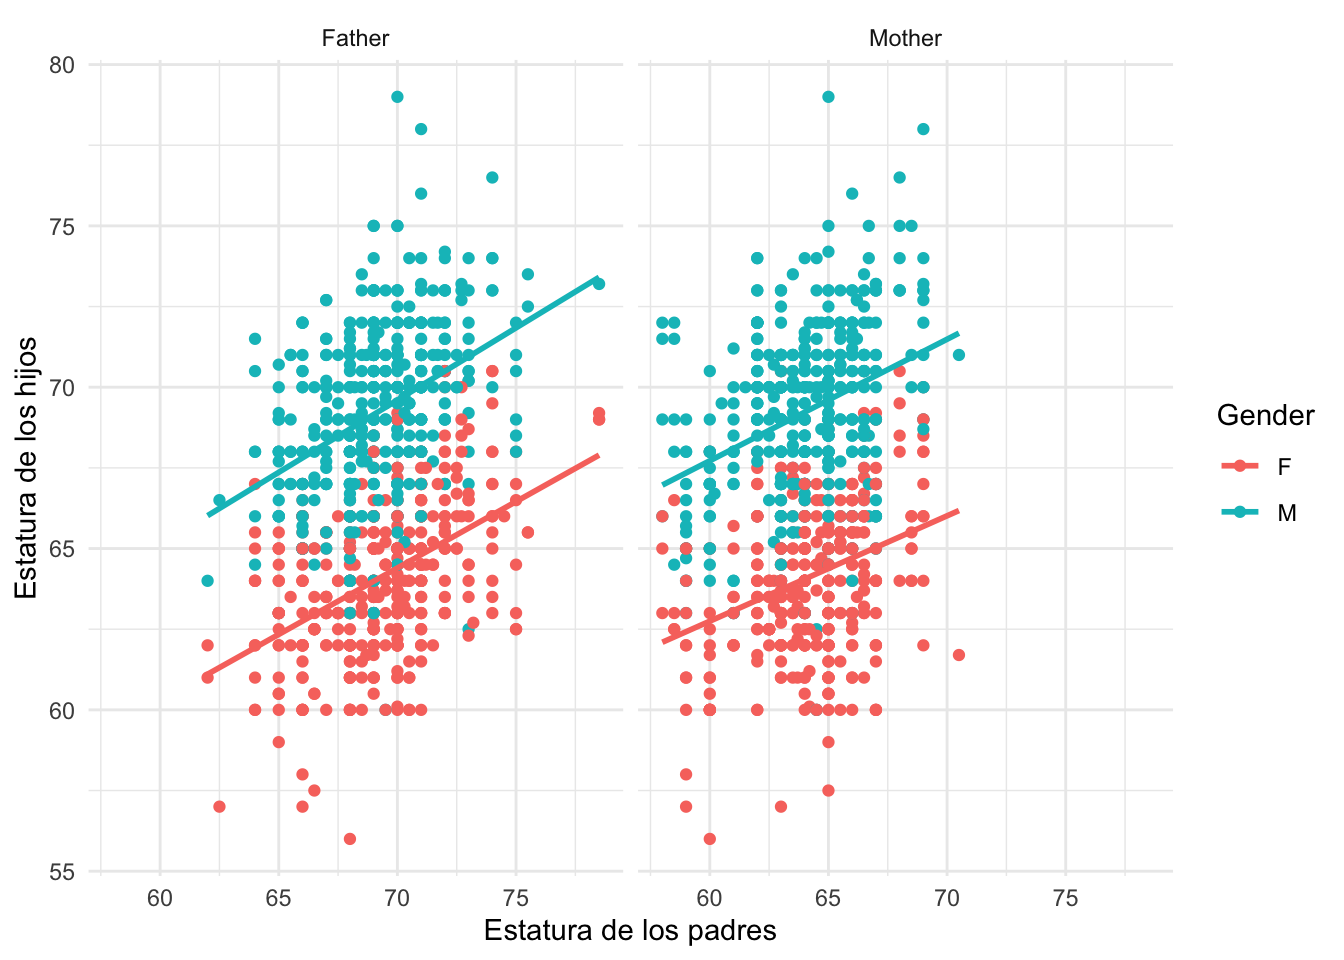
\includegraphics{02-anova_files/figure-latex/unnamed-chunk-9-1.pdf}

Asumimos pues como respuesta la variable \texttt{y=Height}, como regresores las variables \(x_1=\)\texttt{Father} y \(x_2=\)\texttt{Mother} con las estaturas del padre y la madre respectivamente, y con factor de clasificación la variable \(G=\)\texttt{Gender}, con niveles M/F. En principio cabrían posibles interacciones entre los regresores (estaturas del padre y de la madre) y los factores de clasificación (sexo del sujeto). Esto implicaría que las pendientes de relación `estatura padres' versus `estatura hijos' no serían paralelas para los sujetos hombres y mujeres. Planteamos pues el modelo:

\[(y_{ij}|\mu_{ij},\sigma^2) \sim N(\mu_{ij},\sigma^2)\]
con el predictor lineal
\[\eta_{ij}=\mu_{ij}=\beta_0+(\beta_1 + \alpha_{1M}) x_{1j} + (\beta_2+ \alpha_{2M}) x_{2j} + \alpha_M;\ \  j =1,...,n_i; i=M,F\]
donde \(\alpha_M\) es el efecto diferencial global de los hombres frente a las mujeres al predecir la estatura, y \(\alpha_{1M},\alpha_{2M}\) son los efectos diferenciales que afectan a los regresores, y por lo tanto que provocan pendientes distintas al predecir la estatura del sujeto con las de los padres, en función de si este es hombre o mujer.

Asumimos una distribución vaga sobre todos los efectos fijos y \(\tau=1/\sigma^2\), y ajustamos el modelo Gausiano en INLA:

\begin{Shaded}
\begin{Highlighting}[]

\NormalTok{formula }\OtherTok{=}\NormalTok{ Height }\SpecialCharTok{\textasciitilde{}} \DecValTok{1}\SpecialCharTok{+}\NormalTok{(Father}\SpecialCharTok{+}\NormalTok{Mother)}\SpecialCharTok{*}\NormalTok{Gender}
\NormalTok{fit }\OtherTok{=} \FunctionTok{inla}\NormalTok{(formula,}\AttributeTok{family =} \StringTok{"gaussian"}\NormalTok{,}\AttributeTok{data=}\NormalTok{datos)}
\FunctionTok{round}\NormalTok{(fit}\SpecialCharTok{$}\NormalTok{summary.fixed,}\DecValTok{3}\NormalTok{)}
\CommentTok{\#\textgreater{}                  mean    sd 0.025quant 0.5quant 0.975quant}
\CommentTok{\#\textgreater{} (Intercept)    16.652 3.887      9.028   16.652     24.276}
\CommentTok{\#\textgreater{} Father          0.400 0.039      0.324    0.400      0.477}
\CommentTok{\#\textgreater{} Mother          0.307 0.045      0.218    0.307      0.396}
\CommentTok{\#\textgreater{} GenderM         2.707 5.428     {-}7.940    2.707     13.354}
\CommentTok{\#\textgreater{} Father:GenderM  0.012 0.058     {-}0.103    0.012      0.126}
\CommentTok{\#\textgreater{} Mother:GenderM  0.027 0.062     {-}0.096    0.027      0.149}
\CommentTok{\#\textgreater{}                mode kld}
\CommentTok{\#\textgreater{} (Intercept)      NA   0}
\CommentTok{\#\textgreater{} Father           NA   0}
\CommentTok{\#\textgreater{} Mother           NA   0}
\CommentTok{\#\textgreater{} GenderM          NA   0}
\CommentTok{\#\textgreater{} Father:GenderM   NA   0}
\CommentTok{\#\textgreater{} Mother:GenderM   NA   0}
\end{Highlighting}
\end{Shaded}

Observamos que ninguna de las interacciones tienen un efecto a considerar (su RC posterior incluye al cero), de modo que las descartamos y reajustamos el modelo sin ellas.

\[\eta_{ij}=\mu_{ij}=\beta_0+ \beta_1  x_{1j} + \beta_2 x_{2j} + \alpha_M;\ \  j =1,...,n_i; i=M,F.\]

\begin{Shaded}
\begin{Highlighting}[]
\NormalTok{formula }\OtherTok{=}\NormalTok{ Height }\SpecialCharTok{\textasciitilde{}}\NormalTok{ Father}\SpecialCharTok{+}\NormalTok{Mother}\SpecialCharTok{+}\NormalTok{Gender}
\NormalTok{fit }\OtherTok{=} \FunctionTok{inla}\NormalTok{(formula,}\AttributeTok{family =} \StringTok{"gaussian"}\NormalTok{,}\AttributeTok{data=}\NormalTok{datos,}
        \AttributeTok{control.predictor=}\FunctionTok{list}\NormalTok{(}\AttributeTok{compute=}\ConstantTok{TRUE}\NormalTok{),}
         \AttributeTok{control.compute=}\FunctionTok{list}\NormalTok{(}\AttributeTok{return.marginals.predictor=}\ConstantTok{TRUE}\NormalTok{,}
                              \AttributeTok{dic =} \ConstantTok{TRUE}\NormalTok{, }\AttributeTok{waic =} \ConstantTok{TRUE}\NormalTok{))}
\FunctionTok{round}\NormalTok{(fit}\SpecialCharTok{$}\NormalTok{summary.fixed,}\DecValTok{3}\NormalTok{)}
\CommentTok{\#\textgreater{}               mean    sd 0.025quant 0.5quant 0.975quant}
\CommentTok{\#\textgreater{} (Intercept) 15.345 2.746      9.958   15.345     20.732}
\CommentTok{\#\textgreater{} Father       0.406 0.029      0.349    0.406      0.463}
\CommentTok{\#\textgreater{} Mother       0.321 0.031      0.260    0.321      0.383}
\CommentTok{\#\textgreater{} GenderM      5.226 0.144      4.943    5.226      5.508}
\CommentTok{\#\textgreater{}             mode kld}
\CommentTok{\#\textgreater{} (Intercept)   NA   0}
\CommentTok{\#\textgreater{} Father        NA   0}
\CommentTok{\#\textgreater{} Mother        NA   0}
\CommentTok{\#\textgreater{} GenderM       NA   0}
\end{Highlighting}
\end{Shaded}

Ahora todos los efectos fijos son relevantes para predecir la estatura de los hijos. Utilizamos este modelo para derivar las inferencias.

Representamos a continuación en la Figura \ref(fig:galton1) las distribuciones posteriores de los efectos fijos:

\begin{Shaded}
\begin{Highlighting}[]
\NormalTok{fixed}\OtherTok{=}\FunctionTok{names}\NormalTok{(fit}\SpecialCharTok{$}\NormalTok{marginals.fixed)}
\NormalTok{g}\OtherTok{=}\FunctionTok{list}\NormalTok{()}
\ControlFlowTok{for}\NormalTok{(i }\ControlFlowTok{in} \DecValTok{1}\SpecialCharTok{:}\FunctionTok{length}\NormalTok{(fixed))\{}
\NormalTok{  g[[i]]}\OtherTok{=}\FunctionTok{ggplot}\NormalTok{(}\FunctionTok{as.data.frame}\NormalTok{(fit}\SpecialCharTok{$}\NormalTok{marginals.fixed[[i]]),}\FunctionTok{aes}\NormalTok{(}\AttributeTok{x=}\NormalTok{x,}\AttributeTok{y=}\NormalTok{y))}\SpecialCharTok{+}
    \FunctionTok{geom\_line}\NormalTok{()}\SpecialCharTok{+}
    \FunctionTok{geom\_vline}\NormalTok{(}\AttributeTok{xintercept=}\NormalTok{fit}\SpecialCharTok{$}\NormalTok{summary.fixed}\SpecialCharTok{$}\NormalTok{mean[i],}\AttributeTok{linetype=}\StringTok{"dashed"}\NormalTok{)}\SpecialCharTok{+}
    \FunctionTok{geom\_vline}\NormalTok{(}\AttributeTok{xintercept=}\NormalTok{fit}\SpecialCharTok{$}\NormalTok{summary.fixed[i,}\DecValTok{3}\NormalTok{],}\AttributeTok{linetype=}\StringTok{"dotted"}\NormalTok{)}\SpecialCharTok{+}
    \FunctionTok{geom\_vline}\NormalTok{(}\AttributeTok{xintercept=}\NormalTok{fit}\SpecialCharTok{$}\NormalTok{summary.fixed[i,}\DecValTok{5}\NormalTok{],}\AttributeTok{linetype=}\StringTok{"dotted"}\NormalTok{)}\SpecialCharTok{+}
    \FunctionTok{labs}\NormalTok{(}\AttributeTok{x=}\NormalTok{fixed[i],}\AttributeTok{y=}\StringTok{"D.posterior"}\NormalTok{)}
\NormalTok{\}}
\FunctionTok{grid.arrange}\NormalTok{(g[[}\DecValTok{1}\NormalTok{]],g[[}\DecValTok{2}\NormalTok{]],g[[}\DecValTok{3}\NormalTok{]],g[[}\DecValTok{4}\NormalTok{]],}\AttributeTok{ncol=}\DecValTok{2}\NormalTok{)}
\end{Highlighting}
\end{Shaded}

\begin{figure}
\centering
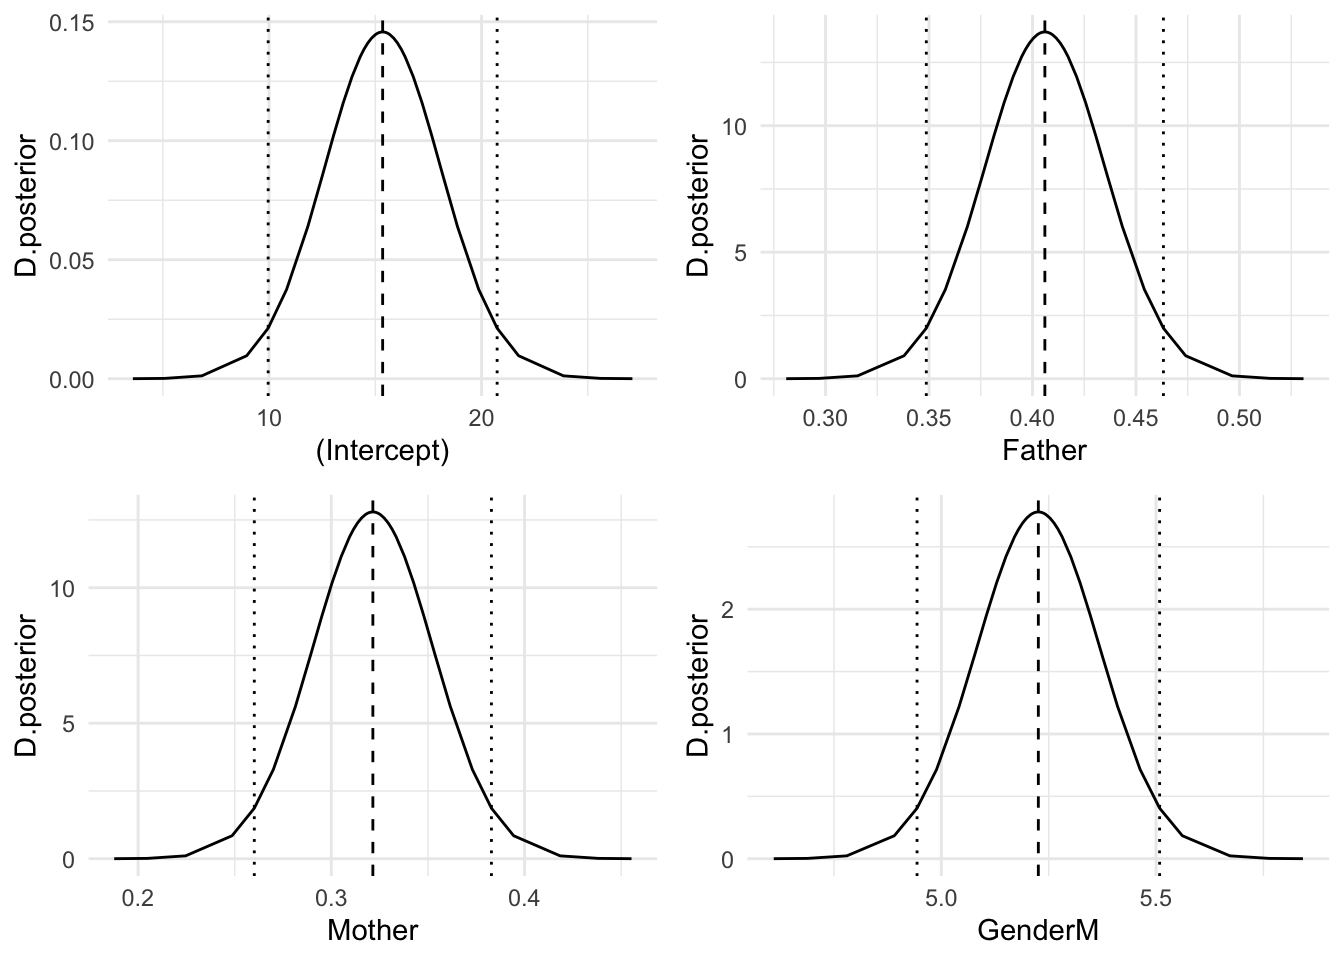
\includegraphics{02-anova_files/figure-latex/galton1-1.pdf}
\caption{\label{fig:galton1}Distribución posterior de los efectos fijos}
\end{figure}

En media observamos que la estatura de los hombres es 5.23 unidades superior a la de las mujeres.

Con estas distribuciones podemos calcular cualquier probabilidad, como por ejemplo,la probabilidad de que la estatura de un hombre supere en 5 unidades a la de una mujer, independientemente de cómo sean sus padres:

\begin{Shaded}
\begin{Highlighting}[]
\DecValTok{1}\SpecialCharTok{{-}}\FunctionTok{inla.pmarginal}\NormalTok{(}\DecValTok{5}\NormalTok{,fit}\SpecialCharTok{$}\NormalTok{marginals.fixed}\SpecialCharTok{$}\StringTok{"GenderM"}\NormalTok{)}
\CommentTok{\#\textgreater{} [1] 0.9414591}
\end{Highlighting}
\end{Shaded}

Podemos acceder a las distribuciones posteriores de la estatura esperada de un sujeto concreto y posicionar las estaturas de sus padres, que se muestran en la Figura \ref{fig:galton2}

\begin{Shaded}
\begin{Highlighting}[]
\CommentTok{\# la predicción del predictor lineal para cada sujeto es:}
\NormalTok{pred}\OtherTok{\textless{}{-}}\NormalTok{fit}\SpecialCharTok{$}\NormalTok{marginals.linear.predictor}
\CommentTok{\# que en este caso coincide con los valores ajustados}
\NormalTok{fitted}\OtherTok{\textless{}{-}}\NormalTok{fit}\SpecialCharTok{$}\NormalTok{marginals.fitted.values}
\FunctionTok{ggplot}\NormalTok{(}\FunctionTok{as.data.frame}\NormalTok{(pred}\SpecialCharTok{$}\NormalTok{Predictor}\FloatTok{.1}\NormalTok{),}\FunctionTok{aes}\NormalTok{(}\AttributeTok{x=}\NormalTok{x,}\AttributeTok{y=}\NormalTok{y))}\SpecialCharTok{+}
  \FunctionTok{geom\_line}\NormalTok{()}\SpecialCharTok{+}
  \FunctionTok{labs}\NormalTok{(}\AttributeTok{x=}\StringTok{"Estatura media del sujeto 1"}\NormalTok{,}\AttributeTok{y=}\StringTok{"D.posterior"}\NormalTok{)}\SpecialCharTok{+}
  \FunctionTok{geom\_vline}\NormalTok{(}\AttributeTok{xintercept=}\NormalTok{fit}\SpecialCharTok{$}\NormalTok{summary.fitted.values}\SpecialCharTok{$}\NormalTok{mean[}\DecValTok{1}\NormalTok{],}\AttributeTok{linetype=}\StringTok{"dashed"}\NormalTok{)}\SpecialCharTok{+}
  \FunctionTok{geom\_vline}\NormalTok{(}\AttributeTok{xintercept=}\NormalTok{datos}\SpecialCharTok{$}\NormalTok{Father[}\DecValTok{1}\NormalTok{],}\AttributeTok{linetype=}\StringTok{"dashed"}\NormalTok{,}\AttributeTok{color=}\StringTok{"blue"}\NormalTok{)}\SpecialCharTok{+}
  \FunctionTok{geom\_vline}\NormalTok{(}\AttributeTok{xintercept=}\NormalTok{datos}\SpecialCharTok{$}\NormalTok{Mother[}\DecValTok{1}\NormalTok{],}\AttributeTok{linetype=}\StringTok{"dashed"}\NormalTok{,}\AttributeTok{color=}\StringTok{"pink"}\NormalTok{)}\SpecialCharTok{+}
  \FunctionTok{annotate}\NormalTok{(}\StringTok{"text"}\NormalTok{,}\AttributeTok{x=}\NormalTok{datos}\SpecialCharTok{$}\NormalTok{Mother[}\DecValTok{1}\NormalTok{]}\SpecialCharTok{+}\DecValTok{1}\NormalTok{,}\AttributeTok{y=}\DecValTok{1}\NormalTok{,}\AttributeTok{label=}\StringTok{"Madre"}\NormalTok{)}\SpecialCharTok{+}
  \FunctionTok{annotate}\NormalTok{(}\StringTok{"text"}\NormalTok{,}\AttributeTok{x=}\NormalTok{datos}\SpecialCharTok{$}\NormalTok{Father[}\DecValTok{1}\NormalTok{]}\SpecialCharTok{{-}}\DecValTok{1}\NormalTok{,}\AttributeTok{y=}\DecValTok{1}\NormalTok{,}\AttributeTok{label=}\StringTok{"Padre"}\NormalTok{)}
\end{Highlighting}
\end{Shaded}

\begin{figure}
\centering
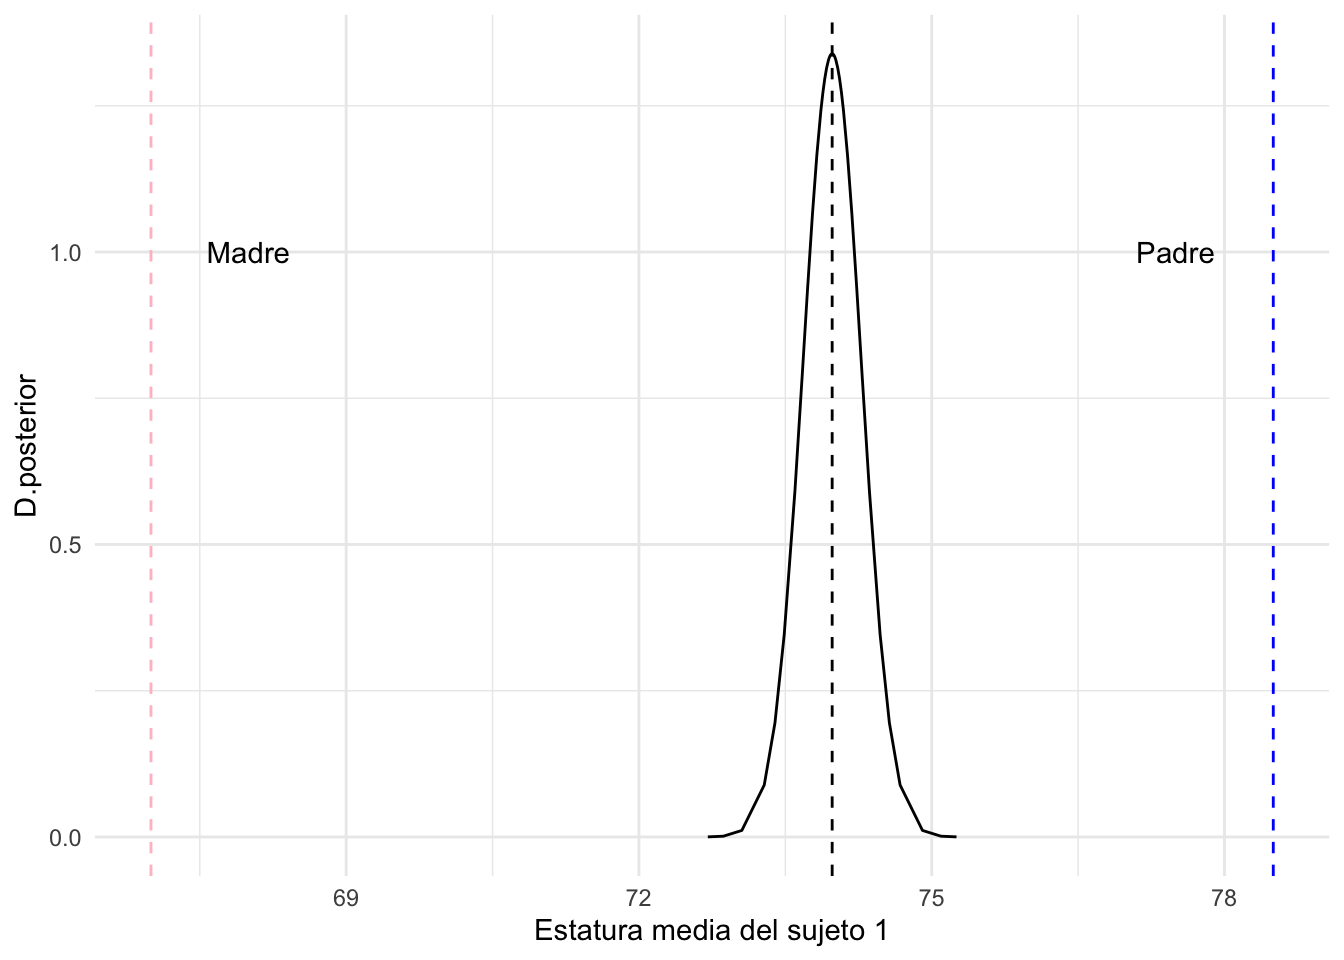
\includegraphics{02-anova_files/figure-latex/galton2-1.pdf}
\caption{\label{fig:galton2}Predicción de la estatura del primer sujeto en la muestra}
\end{figure}

Podemos ir más allá, prediciendo la estatura (esperada) de un sujeto, sea hombre o mujer, cuando su padre mide 1.75m (68.9 pulgadas) y su madre 1.70m (66.9 pulgadas). Expresamos los resultados en centímetros.

\begin{Shaded}
\begin{Highlighting}[]
\NormalTok{new.data}\OtherTok{=}\FunctionTok{data.frame}\NormalTok{(}\AttributeTok{Father=}\FunctionTok{c}\NormalTok{(}\FloatTok{68.9}\NormalTok{,}\FloatTok{68.9}\NormalTok{),}
                    \AttributeTok{Mother=}\FunctionTok{c}\NormalTok{(}\FloatTok{66.9}\NormalTok{,}\FloatTok{66.9}\NormalTok{),}
                    \AttributeTok{Gender=}\FunctionTok{c}\NormalTok{(}\StringTok{"M"}\NormalTok{,}\StringTok{"F"}\NormalTok{),}
                    \AttributeTok{Height=}\FunctionTok{c}\NormalTok{(}\ConstantTok{NA}\NormalTok{,}\ConstantTok{NA}\NormalTok{))}
\NormalTok{datos.combinado }\OtherTok{\textless{}{-}} \FunctionTok{rbind}\NormalTok{(datos, }\FunctionTok{data.frame}\NormalTok{(}\AttributeTok{Family=}\FunctionTok{c}\NormalTok{(}\ConstantTok{NA}\NormalTok{,}\ConstantTok{NA}\NormalTok{),new.data,}\AttributeTok{Kids=}\FunctionTok{c}\NormalTok{(}\ConstantTok{NA}\NormalTok{,}\ConstantTok{NA}\NormalTok{)))}

\DocumentationTok{\#\# creamos un vector con NA\textquotesingle{}s para observaciones y 1\textquotesingle{}s para predicciones}
\NormalTok{datos.indicador }\OtherTok{\textless{}{-}} \FunctionTok{c}\NormalTok{(}\FunctionTok{rep}\NormalTok{(}\ConstantTok{NA}\NormalTok{, }\FunctionTok{nrow}\NormalTok{(datos)), }\FunctionTok{rep}\NormalTok{(}\DecValTok{1}\NormalTok{, }\FunctionTok{nrow}\NormalTok{(new.data)))}
\DocumentationTok{\#\# reajustamos el modelo añadiendo la opción de predicción de datos}
\NormalTok{fit.pred }\OtherTok{\textless{}{-}} \FunctionTok{inla}\NormalTok{(formula, }\AttributeTok{data =}\NormalTok{ datos.combinado, }
                 \AttributeTok{control.compute=}\FunctionTok{list}\NormalTok{(}\AttributeTok{return.marginals.predictor=}\ConstantTok{TRUE}\NormalTok{),}
                 \AttributeTok{control.predictor =} \FunctionTok{list}\NormalTok{(}\AttributeTok{link =}\NormalTok{ datos.indicador))}
\DocumentationTok{\#\# y describimos los valores ajustados para los escenarios añadidos}
\FunctionTok{round}\NormalTok{(fit.pred}\SpecialCharTok{$}\NormalTok{summary.fitted.values[(}\FunctionTok{nrow}\NormalTok{(datos)}\SpecialCharTok{+}\DecValTok{1}\NormalTok{)}\SpecialCharTok{:}\FunctionTok{nrow}\NormalTok{(datos.combinado),]}\SpecialCharTok{*}\FloatTok{2.54}\NormalTok{,}\DecValTok{1}\NormalTok{)}
\CommentTok{\#\textgreater{}                       mean  sd 0.025quant 0.5quant}
\CommentTok{\#\textgreater{} fitted.Predictor.899 177.9 0.3      177.3    177.9}
\CommentTok{\#\textgreater{} fitted.Predictor.900 164.7 0.3      164.0    164.7}
\CommentTok{\#\textgreater{}                      0.975quant mode}
\CommentTok{\#\textgreater{} fitted.Predictor.899      178.6   NA}
\CommentTok{\#\textgreater{} fitted.Predictor.900      165.3   NA}
\end{Highlighting}
\end{Shaded}

También graficar las distribuciones posteriores y calcular las probabilidades, por ejemplo, de que dicho sujeto supere el 1.65m si es mujer, o el 1.78m si es hombre (Figura \ref{fig:galton3}).

\begin{Shaded}
\begin{Highlighting}[]
\CommentTok{\# Distribuciones predictivas}
\NormalTok{pred.M}\OtherTok{=}\FunctionTok{as.data.frame}\NormalTok{(fit.pred}\SpecialCharTok{$}\NormalTok{marginals.fitted.values[[(}\FunctionTok{nrow}\NormalTok{(datos)}\SpecialCharTok{+}\DecValTok{1}\NormalTok{)]])}\SpecialCharTok{*}\FloatTok{2.54}
\NormalTok{pred.F}\OtherTok{=}\FunctionTok{as.data.frame}\NormalTok{(fit.pred}\SpecialCharTok{$}\NormalTok{marginals.fitted.values[[(}\FunctionTok{nrow}\NormalTok{(datos)}\SpecialCharTok{+}\DecValTok{2}\NormalTok{)]])}\SpecialCharTok{*}\FloatTok{2.54}
\NormalTok{d.pred}\OtherTok{=}\FunctionTok{rbind}\NormalTok{(pred.M,pred.F)}

\CommentTok{\# atributo Gender}
\NormalTok{d.pred}\SpecialCharTok{$}\NormalTok{Gender}\OtherTok{=}\FunctionTok{rep}\NormalTok{(}\FunctionTok{c}\NormalTok{(}\StringTok{"M"}\NormalTok{,}\StringTok{"F"}\NormalTok{),}\FunctionTok{c}\NormalTok{(}\FunctionTok{nrow}\NormalTok{(pred.M),}\FunctionTok{nrow}\NormalTok{(pred.F)))}
\CommentTok{\# objetivo de estatura}
\NormalTok{d.pred}\SpecialCharTok{$}\NormalTok{obj}\OtherTok{=}\FunctionTok{rep}\NormalTok{(}\FunctionTok{c}\NormalTok{(}\DecValTok{178}\NormalTok{,}\DecValTok{165}\NormalTok{),}\FunctionTok{c}\NormalTok{(}\FunctionTok{nrow}\NormalTok{(pred.M),}\FunctionTok{nrow}\NormalTok{(pred.F)))}

\CommentTok{\# cálculo de probabilidades}
\NormalTok{p165F}\OtherTok{=}\FunctionTok{round}\NormalTok{(}\DecValTok{1}\SpecialCharTok{{-}}\FunctionTok{inla.pmarginal}\NormalTok{(}\DecValTok{165}\NormalTok{,pred.F),}\DecValTok{2}\NormalTok{)}
\FunctionTok{cat}\NormalTok{(}\FunctionTok{paste}\NormalTok{(}\StringTok{"Pr(estatura\textgreater{}165|mujer,padre=175,madre=170)="}\NormalTok{,p165F))}
\CommentTok{\#\textgreater{} Pr(estatura\textgreater{}165|mujer,padre=175,madre=170)= 0.16}
\FunctionTok{cat}\NormalTok{(}\StringTok{"}\SpecialCharTok{\textbackslash{}n}\StringTok{"}\NormalTok{)}
\NormalTok{p178M}\OtherTok{=}\FunctionTok{round}\NormalTok{(}\DecValTok{1}\SpecialCharTok{{-}}\FunctionTok{inla.pmarginal}\NormalTok{(}\DecValTok{178}\NormalTok{,pred.M),}\DecValTok{2}\NormalTok{)}
\FunctionTok{cat}\NormalTok{(}\FunctionTok{paste}\NormalTok{(}\StringTok{"Pr(estatura\textgreater{}178|hombre,padre=175,madre=170)="}\NormalTok{,p178M))}
\CommentTok{\#\textgreater{} Pr(estatura\textgreater{}178|hombre,padre=175,madre=170)= 0.42}

\NormalTok{d.pred}\SpecialCharTok{$}\NormalTok{prob}\OtherTok{=}\FunctionTok{rep}\NormalTok{(}\FunctionTok{c}\NormalTok{(p178M,p165F),}\FunctionTok{c}\NormalTok{(}\FunctionTok{nrow}\NormalTok{(pred.M),}\FunctionTok{nrow}\NormalTok{(pred.F)))}


\FunctionTok{ggplot}\NormalTok{(d.pred,}\FunctionTok{aes}\NormalTok{(}\AttributeTok{x=}\NormalTok{x,}\AttributeTok{y=}\NormalTok{y))}\SpecialCharTok{+}
  \FunctionTok{geom\_line}\NormalTok{(}\FunctionTok{aes}\NormalTok{(}\AttributeTok{color=}\NormalTok{Gender))}\SpecialCharTok{+}
  \FunctionTok{geom\_vline}\NormalTok{(}\FunctionTok{aes}\NormalTok{(}\AttributeTok{xintercept=}\NormalTok{obj),}\AttributeTok{linetype=}\StringTok{"dashed"}\NormalTok{)}\SpecialCharTok{+}
  \FunctionTok{facet\_wrap}\NormalTok{(}\FunctionTok{vars}\NormalTok{(Gender),}\AttributeTok{scales=}\StringTok{"free"}\NormalTok{)}\SpecialCharTok{+}
  \FunctionTok{labs}\NormalTok{(}\AttributeTok{x=}\StringTok{"Estatura"}\NormalTok{,}\AttributeTok{y=}\StringTok{"D.posterior"}\NormalTok{)}\SpecialCharTok{+}
    \FunctionTok{theme}\NormalTok{(}\AttributeTok{legend.position =} \StringTok{"none"}\NormalTok{)}
\end{Highlighting}
\end{Shaded}

\begin{figure}
\centering
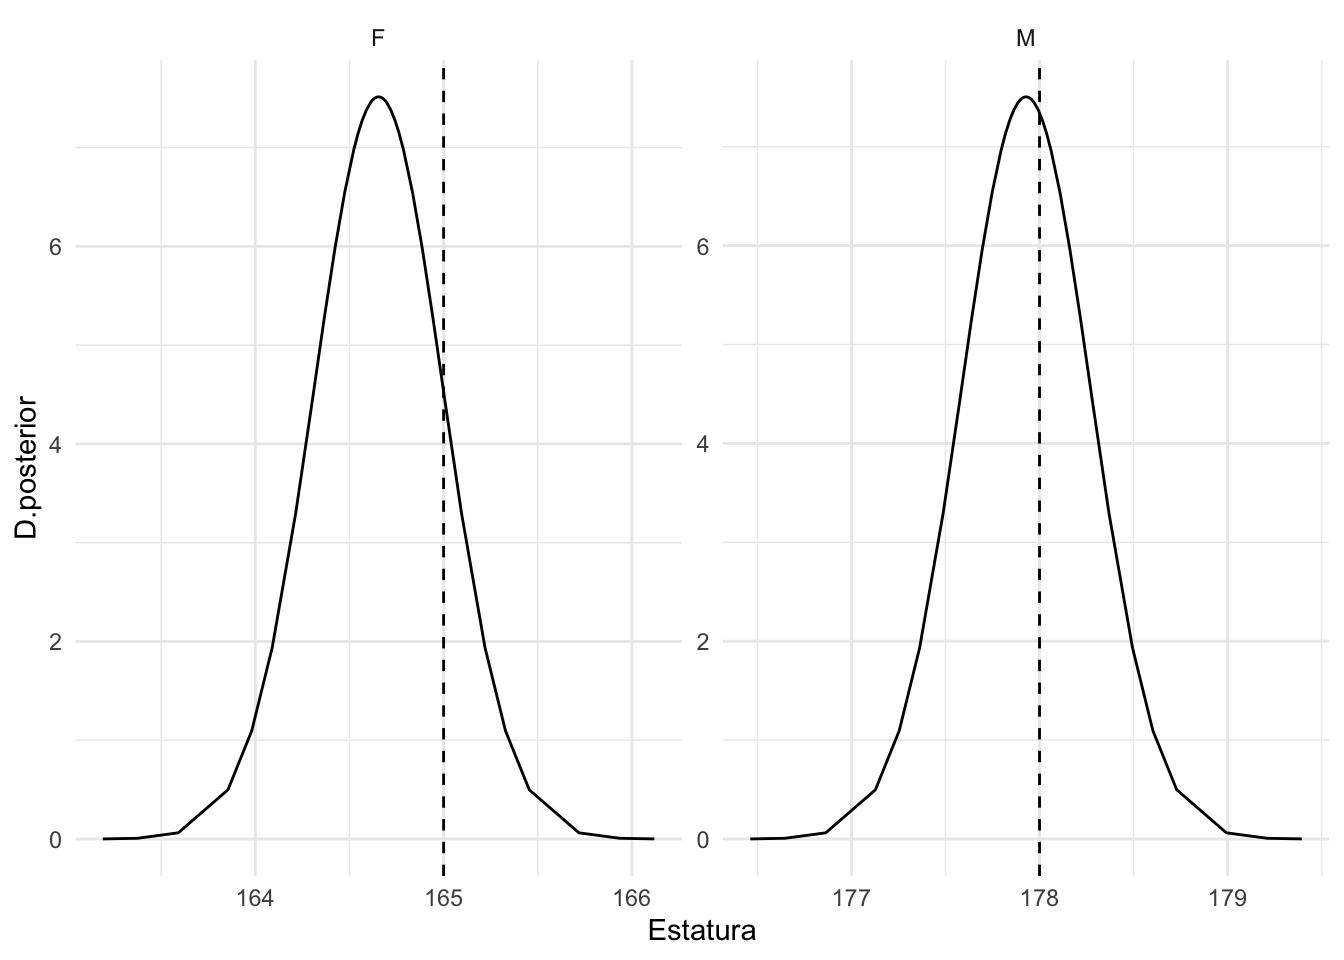
\includegraphics{02-anova_files/figure-latex/galton3-1.pdf}
\caption{\label{fig:galton3}Distribución posterior de la estatura de un sujeto cuyo padre mide 1,75cm y madre 1,07cm.}
\end{figure}

Podríamos también, modificar las especificaciones a priori sobre los parámetros \(\beta_0\) y \(\beta_1\) mediante el comando \texttt{control.fixed}. Por ejemplo, queremos asumir a priori \(\beta_0\sim N(0,10^4)\) y \(\beta_1\sim N(0,100)\) y ver cómo afecta a las inferencias.

\begin{Shaded}
\begin{Highlighting}[]
\NormalTok{fit}\OtherTok{\textless{}{-}}\FunctionTok{inla}\NormalTok{(formula,}\AttributeTok{family=}\StringTok{"gaussian"}\NormalTok{,}\AttributeTok{data=}\NormalTok{datos,}
                   \AttributeTok{control.fixed=}\FunctionTok{list}\NormalTok{(}\AttributeTok{mean=}\DecValTok{0}\NormalTok{,}\AttributeTok{prec=}\FloatTok{0.01}\NormalTok{,}
                   \AttributeTok{mean.intercept=}\DecValTok{0}\NormalTok{, }\AttributeTok{prec.intercept=}\FloatTok{0.0001}\NormalTok{))}
\FunctionTok{round}\NormalTok{(fit}\SpecialCharTok{$}\NormalTok{summary.fixed,}\DecValTok{3}\NormalTok{)}
\CommentTok{\#\textgreater{}               mean    sd 0.025quant 0.5quant 0.975quant}
\CommentTok{\#\textgreater{} (Intercept) 15.335 2.746      9.950   15.335     20.721}
\CommentTok{\#\textgreater{} Father       0.406 0.029      0.349    0.406      0.463}
\CommentTok{\#\textgreater{} Mother       0.322 0.031      0.260    0.322      0.383}
\CommentTok{\#\textgreater{} GenderM      5.225 0.144      4.942    5.225      5.507}
\CommentTok{\#\textgreater{}             mode kld}
\CommentTok{\#\textgreater{} (Intercept)   NA   0}
\CommentTok{\#\textgreater{} Father        NA   0}
\CommentTok{\#\textgreater{} Mother        NA   0}
\CommentTok{\#\textgreater{} GenderM       NA   0}
\end{Highlighting}
\end{Shaded}

Si queremos especificar medias a priori diferentes para los coeficientes de los distintos regresores, hemos de especificarlos con listas.

\begin{Shaded}
\begin{Highlighting}[]
\NormalTok{fit }\OtherTok{=} \FunctionTok{inla}\NormalTok{(formula,}\AttributeTok{family =} \StringTok{"gaussian"}\NormalTok{,}\AttributeTok{data=}\NormalTok{datos,}
                   \AttributeTok{control.fixed=}\FunctionTok{list}\NormalTok{(}\AttributeTok{mean=}\FunctionTok{list}\NormalTok{(}\AttributeTok{Father=}\FloatTok{0.2}\NormalTok{,}\AttributeTok{Mother=}\FloatTok{0.1}\NormalTok{)))}
\FunctionTok{round}\NormalTok{(fit}\SpecialCharTok{$}\NormalTok{summary.fixed,}\DecValTok{3}\NormalTok{)}
\CommentTok{\#\textgreater{}               mean    sd 0.025quant 0.5quant 0.975quant}
\CommentTok{\#\textgreater{} (Intercept) 15.345 2.746      9.958   15.345     20.732}
\CommentTok{\#\textgreater{} Father       0.406 0.029      0.349    0.406      0.463}
\CommentTok{\#\textgreater{} Mother       0.321 0.031      0.260    0.321      0.383}
\CommentTok{\#\textgreater{} GenderM      5.226 0.144      4.943    5.226      5.508}
\CommentTok{\#\textgreater{}             mode kld}
\CommentTok{\#\textgreater{} (Intercept)   NA   0}
\CommentTok{\#\textgreater{} Father        NA   0}
\CommentTok{\#\textgreater{} Mother        NA   0}
\CommentTok{\#\textgreater{} GenderM       NA   0}
\end{Highlighting}
\end{Shaded}

Si queremos modificar la especificación de la prior en \(\sigma^2\), o lo que es equivalente, en la precisión \(\tau\), con la distribución \(log(\tau) \sim N(0,1)\) en lugar de \(\tau \sim Ga(1,10^{-5})\), vemos cómo afecta a la inferencia posterior sobre la precisión.

\begin{Shaded}
\begin{Highlighting}[]
\NormalTok{fit\_n }\OtherTok{=} \FunctionTok{inla}\NormalTok{(formula,}\AttributeTok{family=}\StringTok{"gaussian"}\NormalTok{, }\AttributeTok{data=}\NormalTok{datos,}
                   \AttributeTok{control.family=}\FunctionTok{list}\NormalTok{(}\AttributeTok{hyper=}\FunctionTok{list}\NormalTok{(}
                     \AttributeTok{prec=}\FunctionTok{list}\NormalTok{(}\AttributeTok{prior=}\StringTok{"gaussian"}\NormalTok{,}\AttributeTok{param=}\FunctionTok{c}\NormalTok{(}\DecValTok{0}\NormalTok{,}\DecValTok{1}\NormalTok{)))))}
\CommentTok{\# con el modelo log{-}gamma para precisión}
\FunctionTok{round}\NormalTok{(fit}\SpecialCharTok{$}\NormalTok{summary.hyperpar,}\DecValTok{3}\NormalTok{)}
\CommentTok{\#\textgreater{}                                          mean   sd}
\CommentTok{\#\textgreater{} Precision for the Gaussian observations 0.216 0.01}
\CommentTok{\#\textgreater{}                                         0.025quant 0.5quant}
\CommentTok{\#\textgreater{} Precision for the Gaussian observations      0.197    0.216}
\CommentTok{\#\textgreater{}                                         0.975quant mode}
\CommentTok{\#\textgreater{} Precision for the Gaussian observations      0.236   NA}
\CommentTok{\# con el modelo normal para precisión}
\FunctionTok{round}\NormalTok{(fit\_n}\SpecialCharTok{$}\NormalTok{summary.hyperpar,}\DecValTok{3}\NormalTok{)}
\CommentTok{\#\textgreater{}                                          mean   sd}
\CommentTok{\#\textgreater{} Precision for the Gaussian observations 0.216 0.01}
\CommentTok{\#\textgreater{}                                         0.025quant 0.5quant}
\CommentTok{\#\textgreater{} Precision for the Gaussian observations      0.197    0.216}
\CommentTok{\#\textgreater{}                                         0.975quant mode}
\CommentTok{\#\textgreater{} Precision for the Gaussian observations      0.237   NA}
\end{Highlighting}
\end{Shaded}

Cuando tenemos información previa disponible sobre la variación de los datos, será generalmente más intuitivo expresarla en términos de la desviación estándar \(\sigma\). Bastará con conseguir la equivalencia en la escala de \(log(\tau)\) para incluirla en el modelo. Por ejemplo, si sabemos que la desviación típica está entre 2 y 14, \(\sigma \sim Unif(2,14)\), podemos calcular una prior para la log-precisión del siguiente modo:

\begin{enumerate}
\def\labelenumi{\arabic{enumi}.}
\tightlist
\item
  simular una muestra de \(\sigma \sim Unif(2,14)\)
\item
  transformar a precisiones
\item
  calcular los parámetros de la Gamma para la precisión, a partir de su media y varianza
\end{enumerate}

Hacemos los cálculos y graficamos la prior en la Figura \ref{fig:galton4}.

\begin{Shaded}
\begin{Highlighting}[]
\CommentTok{\# parámetros para sigma\textasciitilde{}Un(a1,b1)}
\NormalTok{a1}\OtherTok{\textless{}{-}}\DecValTok{2}
\NormalTok{b1}\OtherTok{\textless{}{-}}\DecValTok{14}
\CommentTok{\# simulamos sigma de una distribución Unif(a1,b1)}
\NormalTok{sigma}\OtherTok{\textless{}{-}}\FunctionTok{runif}\NormalTok{(}\AttributeTok{n=}\DecValTok{10000}\NormalTok{,}\AttributeTok{min=}\NormalTok{a1,}\AttributeTok{max=}\NormalTok{b1)}
\CommentTok{\# obtenemos la precisión}
\NormalTok{tau}\OtherTok{\textless{}{-}}\DecValTok{1}\SpecialCharTok{/}\NormalTok{sigma}\SpecialCharTok{\^{}}\DecValTok{2}
\CommentTok{\# Calculamos los parámetros alpha,beta de una distrib. Gamma para la precisión}
\CommentTok{\# mean=alpha/beta; var=alpha/beta\^{}2}
\NormalTok{beta}\OtherTok{=} \FunctionTok{mean}\NormalTok{(tau)}\SpecialCharTok{/}\FunctionTok{var}\NormalTok{(tau)}
\NormalTok{alpha}\OtherTok{\textless{}{-}}\FunctionTok{mean}\NormalTok{(tau)}\SpecialCharTok{*}\NormalTok{beta}
\CommentTok{\# dibujamos los valores de la precisión}
\NormalTok{tau.seq}\OtherTok{=}\FunctionTok{sort}\NormalTok{(tau)}
  \CommentTok{\# seq(min(tau),max(tau),length=1000)}
\NormalTok{prior}\OtherTok{=}\FunctionTok{data.frame}\NormalTok{(}\AttributeTok{tau=}\NormalTok{tau.seq,}\AttributeTok{dprior=}\FunctionTok{dgamma}\NormalTok{(tau.seq,alpha,beta))}
\FunctionTok{ggplot}\NormalTok{(prior, }\FunctionTok{aes}\NormalTok{(}\AttributeTok{x=}\NormalTok{tau))}\SpecialCharTok{+}
  \FunctionTok{geom\_histogram}\NormalTok{(}\FunctionTok{aes}\NormalTok{(}\AttributeTok{y=}\NormalTok{..density..),}\AttributeTok{color=}\StringTok{"grey"}\NormalTok{,}\AttributeTok{fill=}\StringTok{"white"}\NormalTok{)}\SpecialCharTok{+}
  \FunctionTok{geom\_line}\NormalTok{(}\FunctionTok{aes}\NormalTok{(}\AttributeTok{y=}\NormalTok{dprior))}
\CommentTok{\#\textgreater{} \textasciigrave{}stat\_bin()\textasciigrave{} using \textasciigrave{}bins = 30\textasciigrave{}. Pick better value with}
\CommentTok{\#\textgreater{} \textasciigrave{}binwidth\textasciigrave{}.}
\end{Highlighting}
\end{Shaded}

\begin{figure}
\centering
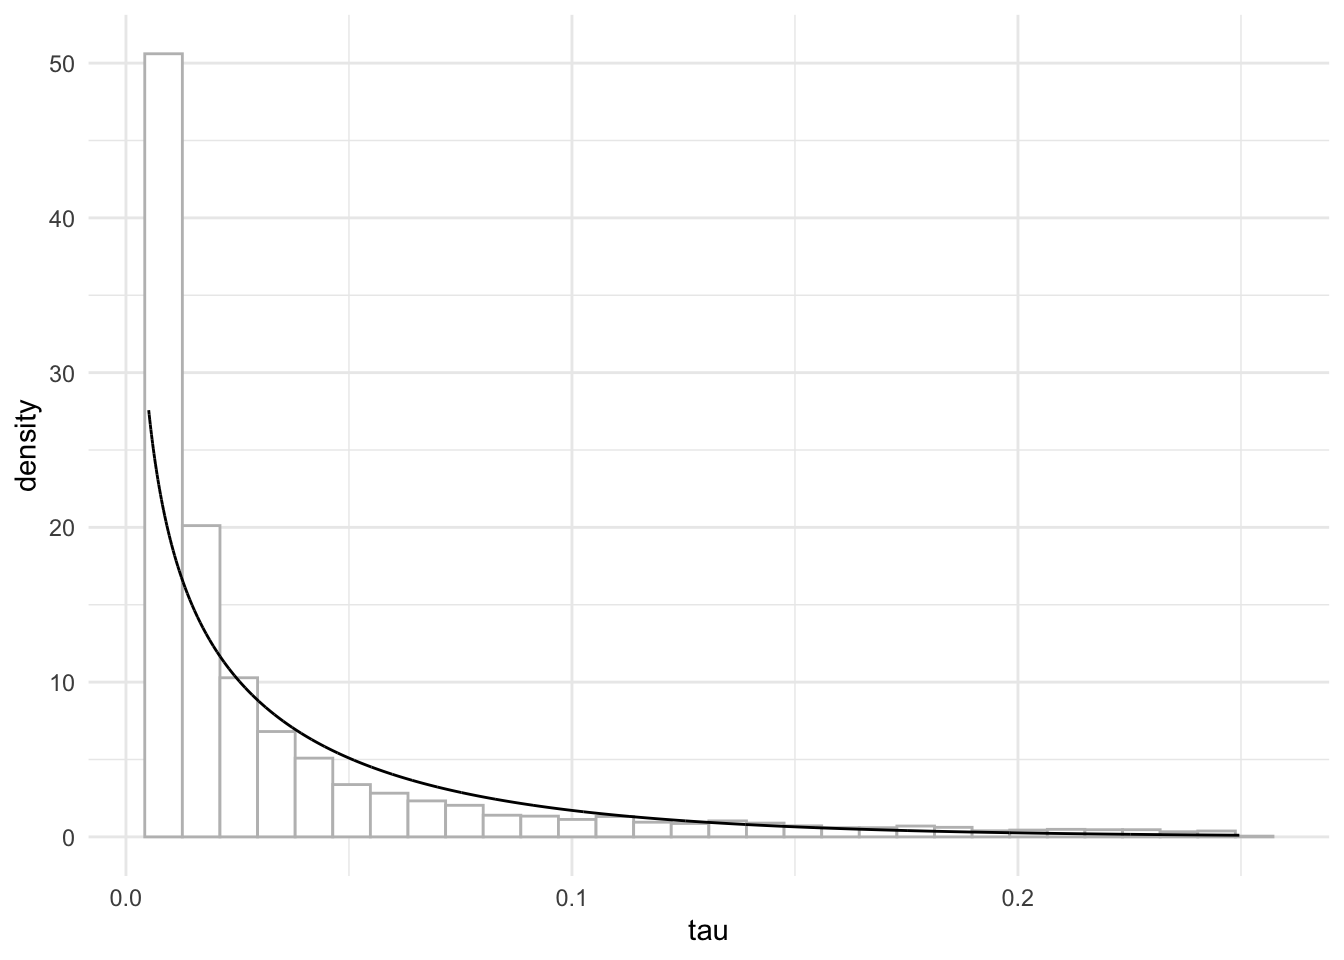
\includegraphics{02-anova_files/figure-latex/galton4-1.pdf}
\caption{\label{fig:galton4}Distribución a prior para tau con sigma \textasciitilde{} Uniforme(2,14)}
\end{figure}

Utilicemos pues esos parámetros para especificar la prior sobre \(\tau\) en INLA:

\begin{Shaded}
\begin{Highlighting}[]
\NormalTok{fit }\OtherTok{=} \FunctionTok{inla}\NormalTok{(formula,}\AttributeTok{family=}\StringTok{"gaussian"}\NormalTok{,}\AttributeTok{data=}\NormalTok{datos,}
                   \AttributeTok{control.family=}\FunctionTok{list}\NormalTok{(}\AttributeTok{hyper=}\FunctionTok{list}\NormalTok{(}
                     \AttributeTok{prec=}\FunctionTok{list}\NormalTok{(}\AttributeTok{prior=}\StringTok{"loggamma"}\NormalTok{,}\AttributeTok{param=}\FunctionTok{c}\NormalTok{(alpha,beta)))))}
\FunctionTok{round}\NormalTok{(fit}\SpecialCharTok{$}\NormalTok{summary.hyperpar,}\DecValTok{3}\NormalTok{)}
\CommentTok{\#\textgreater{}                                          mean   sd}
\CommentTok{\#\textgreater{} Precision for the Gaussian observations 0.214 0.01}
\CommentTok{\#\textgreater{}                                         0.025quant 0.5quant}
\CommentTok{\#\textgreater{} Precision for the Gaussian observations      0.195    0.214}
\CommentTok{\#\textgreater{}                                         0.975quant mode}
\CommentTok{\#\textgreater{} Precision for the Gaussian observations      0.234   NA}
\end{Highlighting}
\end{Shaded}

\hypertarget{efectos-aleatorios}{%
\section{Efectos aleatorios}\label{efectos-aleatorios}}

Desde una perspectiva frecuentista un modelo básico de Anova podría ser un modelo de efectos fijos, pero también de efectos aleatorios. Así por ejemplo el `tratamiento' dado en un ensayo clínico es un efecto relevante para comparar y diferenciar cómo afecta a la respuesta; `tratamiento' sería entonces un efecto fijo, por ser un efecto de interés primario. En otro ejemplo, se han aplicado varios fertilizantes a cultivos en fincas distintas; el interés primario será comparar los fertilizantes, pero la diversidad de fincas solo se ha incluido para introducir variabilidad e incrementar, por supuesto, el número de datos en el estudio; así pues, `fertilizante' será un efecto fijo, pero no es un objetivo comparar las fincas, por lo que se considerará como un efecto aleatorio.

Una variable predictiva, numérica o categórica, entra en el modelo como \textbf{efecto fijo} cuando se piensa que afecta a todas las observaciones del mismo modo, y que su efecto es de interés primario en el estudio.
En un contexto bayesiano un efecto fijo tendrá un coeficiente asociado al que se le asigna a menudo una distribución a priori vaga (mínimo informativa), como una gausiana con media cero y varianza (conocida) grande. En cualquier caso, la distribución a priori que se asume para los efectos fijos es siempre una distribución conocida.

Un \textbf{efecto aleatorio} identifica a variables de tipo categórico que no son de interés primario en la investigación, pero que se considera que añaden incertidumbre y por lo tanto variabilidad a la respuesta. La modelización habitual de los efectos aleatorios es una prior gausiana con media cero y una precisión desconocida, para la que será preciso asignar, así mismo, una distribución a priori. La distribución a priori de los efectos aleatorios tiene parámetros desconocidos, llamados \textbf{hiperparámetros}, a los que habrá que asignar también distribuciones a priori.

Puesto que no salimos del modelo lineal, seguiremos asumiendo una respuesta normal, \emph{gaussian}, con media igual a un predictor lineal \(\mu=\eta=\theta+ Z u\), donde \(Z\) es la correspondiente matriz de diseño para los efectos aleatorios \(z_1, z_2,...\). Se asume además una varianza desconocida \(\sigma^2\).

En INLA la fórmula de predicción de una respuesta \(y\) a partir de un conjunto de efectos aleatorios z1,z2,\ldots{} se especifica como:

\begin{Shaded}
\begin{Highlighting}[]
\NormalTok{formula }\OtherTok{=}\NormalTok{ y }\SpecialCharTok{\textasciitilde{}} \DecValTok{1}  \SpecialCharTok{+} \FunctionTok{f}\NormalTok{(z1, }\AttributeTok{model=}\StringTok{""}\NormalTok{) }\SpecialCharTok{+} \FunctionTok{f}\NormalTok{(z2,}\AttributeTok{model=}\StringTok{""}\NormalTok{) }
\end{Highlighting}
\end{Shaded}

donde la función \(f()\) especifica la relación entre el predictor lineal de la respuesta y los efectos aleatorios \(z\). La función \(f()\) tiene muchos argumentos, que se pueden consultar con el comando \texttt{?f}. El tipo de relación asumida se incluye en el argumento \texttt{model} o modelo latente, que tiene como posibilidades \texttt{names(inla.models()\$latent)}. En el modelo lineal, la opción habitual es \texttt{model="iid"}, que asume efectos aleatorios independientes e idénticamente distribuidos.

\begin{Shaded}
\begin{Highlighting}[]
\FunctionTok{names}\NormalTok{(}\FunctionTok{inla.models}\NormalTok{()}\SpecialCharTok{$}\NormalTok{latent)}
\CommentTok{\#\textgreater{}  [1] "linear"       "iid"          "mec"         }
\CommentTok{\#\textgreater{}  [4] "meb"          "rgeneric"     "cgeneric"    }
\CommentTok{\#\textgreater{}  [7] "rw1"          "rw2"          "crw2"        }
\CommentTok{\#\textgreater{} [10] "seasonal"     "besag"        "besag2"      }
\CommentTok{\#\textgreater{} [13] "bym"          "bym2"         "besagproper" }
\CommentTok{\#\textgreater{} [16] "besagproper2" "fgn"          "fgn2"        }
\CommentTok{\#\textgreater{} [19] "ar1"          "ar1c"         "ar"          }
\CommentTok{\#\textgreater{} [22] "ou"           "intslope"     "generic"     }
\CommentTok{\#\textgreater{} [25] "generic0"     "generic1"     "generic2"    }
\CommentTok{\#\textgreater{} [28] "generic3"     "spde"         "spde2"       }
\CommentTok{\#\textgreater{} [31] "spde3"        "iid1d"        "iid2d"       }
\CommentTok{\#\textgreater{} [34] "iid3d"        "iid4d"        "iid5d"       }
\CommentTok{\#\textgreater{} [37] "iidkd"        "2diid"        "z"           }
\CommentTok{\#\textgreater{} [40] "rw2d"         "rw2diid"      "slm"         }
\CommentTok{\#\textgreater{} [43] "matern2d"     "dmatern"      "copy"        }
\CommentTok{\#\textgreater{} [46] "clinear"      "sigm"         "revsigm"     }
\CommentTok{\#\textgreater{} [49] "log1exp"      "logdist"}
\end{Highlighting}
\end{Shaded}

Veamos cómo ajustar un modelo de efectos aleatorios a partir de un ejemplo sencillo. Comenzamos con la base de datos \texttt{broccoli} en la librería \href{https://cran.r-project.org/web/packages/faraway/faraway.pdf}{\texttt{faraway}}. Varios cultivadores suministran brócoli a una planta de procesamiento de alimentos. La planta da instrucciones a los cultivadores para que empaquen el brócoli en cajas de tamaño estándar. Debe haber 18 racimos de brócoli por caja y cada racimo debe pesar entre 1,33 y 1,5 libras. Debido a que los productores utilizan diferentes variedades, métodos de cultivo, etc., hay cierta variación en el peso de los racimos. El responsable de la planta seleccionó 3 cultivadores al azar y luego 4 cajas al azar suministradas por estos cultivadores. Se seleccionaron 3 racimos de brocoli de cada caja (a modo de repeticiones).

La variable de interés es el peso del racimo de brócoli, en la variable \texttt{wt}. Sin embargo, dado cómo se ha seleccionado la muestra, el objetivo no es ni la comparación entre cultivadores (\texttt{grower}), ni entre cajas (\texttt{box}), asumiendo que tenemos varios racimos (\texttt{cluster}) en cada una de las combinaciones de los anteriores factores. Sin embargo, de manera lógica intuimos que habrá variabilidad entre cajas (efecto aleatorio \texttt{box}) y también entre cultivadores (efecto aleatorio \texttt{grower}), lo que nos conduce a un modelo en el que todos los predictores, \texttt{box} y \texttt{grower} intervienen como efectos aleatorios; la variable \texttt{cluster} la aprovechamos a modo de repeticiones de medidas en una misma caja de un mismo cultivador.

La base de datos cuenta con 36 registros (3 observaciones en cada combinación \texttt{grower-box}.

\[(y_{ijk}|\mu_{ij},\sigma^2 ) \sim N(\mu_{ij},\sigma^2)\]

con \[\eta_{ij} =\mu_{ij}= \theta + \alpha_i^G + \beta_j^B; \ \  i=2,3; j=2,3,4\]
el peso medio que comparten todos los racimos en cada combinación de agricultor-caja: \(k=1,2,3\), y donde \(\alpha^G\) representa el efecto aleatorio asociado al cultivador (\texttt{grower}) y \(\beta^B\) a la caja (\texttt{box}).

Así el vector de efectos latentes está compuesto por el efecto fijo de interceptación \(theta\) y los efectos aleatorios \(u=(\alpha_2^G,\alpha_3^G,\beta_2^B,\beta_3^B,\beta_4^B)\).

El siguiente paso es especificar una distribución a priori sobre los parámetros. INLA por defecto asigna una prior difusa sobre la interceptación \(\theta\) y también sobre la precisión de los datos \(\tau=1/\sigma^2\). Dado que los \(\alpha_i^G\) representan el efecto diferencial asociado al cultivador, es razonable asumir independencia entre todos estos parámetros y una distribución idéntica, centrada en el cero (ante ausencia de información) y con una varianza desconocida. Con esto estamos diciendo que en principio no tenemos información sobre que efectivamente el efecto cultivador sea relevante (media cero), pero sí que añade cierta variabilidad \(\sigma_{\alpha}^2\) a la respuesta. Del mismo modo, se asume que los \(\beta_j^B\) son a priori independientes e idénticamente distribuidos (iid) con una normal centrada en el cero (ante ausencia de información) y con varianza desconocida \(\sigma_{\beta}^2\).

\begin{eqnarray*}
\theta &\sim & N(0,\sigma_{\theta}^2), \ \sigma_{\theta}^2=\infty \\
log(\tau) &\sim & Log-Ga(1,5\cdot 10^{-5})\\
\alpha_i^G & \sim_{iid} & N(0,\sigma_{\alpha}^2), i=2,3 \\
\beta_j^B & \sim_{iid} & N(0,\sigma_{\beta}^2), j=2,3,4
\end{eqnarray*}

Surgen pues, dos nuevos parámetros en las a priori, o hiperparámetros, \(\sigma_{\alpha}^2\) y \(\sigma_{\beta}^2\), a los que también habrá que asignar una distribución a priori. Dado que se trata de varianzas, por defecto INLA asume gammas inversas difusas, o lo que es lo mismo, log-gammas difusas para las precisiones

\begin{eqnarray*}
\tau_{\alpha}=1/\sigma_{\alpha}^2 &\sim & Ga(1,5\cdot 10^{-5}) \\
\tau_{\beta}=1/\sigma_{\beta}^2 &\sim & Ga(1,5\cdot 10^{-5})
\end{eqnarray*}

Surgen pues, tres niveles de especificación del modelo: datos, parámetros e hiperparámetros, que generan un \textbf{modelo jerárquico de tres niveles}, y sobre el que hablaremos más adelante.

\begin{Shaded}
\begin{Highlighting}[]
\FunctionTok{data}\NormalTok{(broccoli, }\AttributeTok{package=}\StringTok{"faraway"}\NormalTok{)}
\FunctionTok{str}\NormalTok{(broccoli)}
\CommentTok{\#\textgreater{} \textquotesingle{}data.frame\textquotesingle{}:    36 obs. of  4 variables:}
\CommentTok{\#\textgreater{}  $ wt     : num  352 369 383 339 367 328 376 359 388 365 ...}
\CommentTok{\#\textgreater{}  $ grower : Factor w/ 3 levels "1","2","3": 1 1 1 2 2 2 3 3 3 1 ...}
\CommentTok{\#\textgreater{}  $ box    : Factor w/ 4 levels "1","2","3","4": 1 1 1 1 1 1 1 1 1 2 ...}
\CommentTok{\#\textgreater{}  $ cluster: Factor w/ 3 levels "1","2","3": 1 2 3 1 2 3 1 2 3 1 ...}
\NormalTok{formula }\OtherTok{=}\NormalTok{ wt }\SpecialCharTok{\textasciitilde{}} \FunctionTok{f}\NormalTok{(grower,}\AttributeTok{model=}\StringTok{"iid"}\NormalTok{)}\SpecialCharTok{+} \FunctionTok{f}\NormalTok{(box,}\AttributeTok{model=}\StringTok{"iid"}\NormalTok{)}
\NormalTok{fit }\OtherTok{=} \FunctionTok{inla}\NormalTok{(formula, }\AttributeTok{family=}\StringTok{"gaussian"}\NormalTok{,}\AttributeTok{data=}\NormalTok{broccoli,}
           \AttributeTok{control.compute =} \FunctionTok{list}\NormalTok{(}\AttributeTok{dic=}\ConstantTok{TRUE}\NormalTok{,}\AttributeTok{waic=}\ConstantTok{TRUE}\NormalTok{))  }
\end{Highlighting}
\end{Shaded}

Cuando queremos mostrar los resultados a posteriori sobre los efectos aleatorios a partir de un ajuste \texttt{fit} con \texttt{inla}, tenemos las siguientes opciones:

\begin{itemize}
\tightlist
\item
  \texttt{fit\$summary.random} resume la inferencia posterior sobre los efectos
  aleatorios
\item
  \texttt{names(fit\$marginals.random)} lista los nombre de todos los efectos aleatorios
\item
  \texttt{fit\$marginals.random} da las distribuciones posteriores marginales de los efectos aleatorios
\end{itemize}

\begin{Shaded}
\begin{Highlighting}[]
\NormalTok{fit}\SpecialCharTok{$}\NormalTok{summary.random}
\CommentTok{\#\textgreater{} $grower}
\CommentTok{\#\textgreater{}   ID          mean          sd   0.025quant      0.5quant}
\CommentTok{\#\textgreater{} 1  1  2.575283e{-}07 0.004709469 {-}0.009322078  2.479812e{-}07}
\CommentTok{\#\textgreater{} 2  2 {-}1.802713e{-}06 0.004709469 {-}0.009324333 {-}1.735883e{-}06}
\CommentTok{\#\textgreater{} 3  3  1.545184e{-}06 0.004709469 {-}0.009320669  1.487901e{-}06}
\CommentTok{\#\textgreater{}    0.975quant mode          kld}
\CommentTok{\#\textgreater{} 1 0.009322642   NA 2.733238e{-}08}
\CommentTok{\#\textgreater{} 2 0.009320387   NA 2.733239e{-}08}
\CommentTok{\#\textgreater{} 3 0.009324051   NA 2.733238e{-}08}
\CommentTok{\#\textgreater{} }
\CommentTok{\#\textgreater{} $box}
\CommentTok{\#\textgreater{}   ID          mean         sd  0.025quant      0.5quant}
\CommentTok{\#\textgreater{} 1  1  2.745375e{-}05 0.01372465 {-}0.02741857  2.289973e{-}05}
\CommentTok{\#\textgreater{} 2  2 {-}1.574019e{-}05 0.01372464 {-}0.02748910 {-}1.312919e{-}05}
\CommentTok{\#\textgreater{} 3  3 {-}6.955020e{-}06 0.01372463 {-}0.02747473 {-}5.801330e{-}06}
\CommentTok{\#\textgreater{} 4  4 {-}4.758694e{-}06 0.01372463 {-}0.02747114 {-}3.969305e{-}06}
\CommentTok{\#\textgreater{}   0.975quant mode          kld}
\CommentTok{\#\textgreater{} 1 0.02750826   NA 9.882400e{-}05}
\CommentTok{\#\textgreater{} 2 0.02743767   NA 9.882047e{-}05}
\CommentTok{\#\textgreater{} 3 0.02745201   NA 9.881908e{-}05}
\CommentTok{\#\textgreater{} 4 0.02745559   NA 9.881890e{-}05}
\end{Highlighting}
\end{Shaded}

Sin embargo, lo relevante en un modelo de efectos aleatorios es la inferencia sobre las varianzas asociadas a los datos, pero también la variabilidad extra que añaden los efectos aleatorios:

\begin{Shaded}
\begin{Highlighting}[]
\NormalTok{fit}\SpecialCharTok{$}\NormalTok{summary.hyperpar}
\CommentTok{\#\textgreater{}                                                 mean}
\CommentTok{\#\textgreater{} Precision for the Gaussian observations 3.839158e{-}03}
\CommentTok{\#\textgreater{} Precision for grower                    2.403323e+04}
\CommentTok{\#\textgreater{} Precision for box                       4.224069e+03}
\CommentTok{\#\textgreater{}                                                   sd}
\CommentTok{\#\textgreater{} Precision for the Gaussian observations 9.327656e{-}04}
\CommentTok{\#\textgreater{} Precision for grower                    2.335509e+04}
\CommentTok{\#\textgreater{} Precision for box                       2.275383e+03}
\CommentTok{\#\textgreater{}                                           0.025quant}
\CommentTok{\#\textgreater{} Precision for the Gaussian observations 2.247165e{-}03}
\CommentTok{\#\textgreater{} Precision for grower                    7.003574e+02}
\CommentTok{\#\textgreater{} Precision for box                       1.174507e+03}
\CommentTok{\#\textgreater{}                                             0.5quant}
\CommentTok{\#\textgreater{} Precision for the Gaussian observations 3.762866e{-}03}
\CommentTok{\#\textgreater{} Precision for grower                    1.650764e+04}
\CommentTok{\#\textgreater{} Precision for box                       3.785638e+03}
\CommentTok{\#\textgreater{}                                           0.975quant mode}
\CommentTok{\#\textgreater{} Precision for the Gaussian observations 5.890322e{-}03   NA}
\CommentTok{\#\textgreater{} Precision for grower                    8.387697e+04   NA}
\CommentTok{\#\textgreater{} Precision for box                       9.847258e+03   NA}
\end{Highlighting}
\end{Shaded}

Vemos que tanto la precisión asociada al efecto aleatorio caja (\texttt{box}), como al efecto cultivador, \texttt{grower}, son muy grandes, lo que implica varianzas muy pequeñas que posiblemente nos permitiría prescindir de dichos efectos aleatorios para ajustar un mejor modelo.Cuando transformamos a escala de desviaciones estándar, tenemos la distribución posterior para los tres tipos de error, representados en la Figura \ref{fig:brocoli2}.

\begin{Shaded}
\begin{Highlighting}[]
\NormalTok{nombres}\OtherTok{=}\FunctionTok{c}\NormalTok{(}\StringTok{"sigma"}\NormalTok{,}\StringTok{"grower"}\NormalTok{,}\StringTok{"box"}\NormalTok{)}
\NormalTok{sigma.post}\OtherTok{=}\FunctionTok{as.data.frame}\NormalTok{(}\FunctionTok{inla.tmarginal}\NormalTok{(}\ControlFlowTok{function}\NormalTok{(tau) tau}\SpecialCharTok{\^{}}\NormalTok{(}\SpecialCharTok{{-}}\DecValTok{1}\SpecialCharTok{/}\DecValTok{2}\NormalTok{),}
\NormalTok{  fit}\SpecialCharTok{$}\NormalTok{marginals.hyperpar[[}\DecValTok{1}\NormalTok{]]))}
\NormalTok{sigma.grower.post }\OtherTok{=}\FunctionTok{as.data.frame}\NormalTok{(}\FunctionTok{inla.tmarginal}\NormalTok{(}\ControlFlowTok{function}\NormalTok{(tau) tau}\SpecialCharTok{\^{}}\NormalTok{(}\SpecialCharTok{{-}}\DecValTok{1}\SpecialCharTok{/}\DecValTok{2}\NormalTok{),}
\NormalTok{  fit}\SpecialCharTok{$}\NormalTok{marginals.hyperpar[[}\DecValTok{2}\NormalTok{]]))}
\NormalTok{sigma.box.post }\OtherTok{=} \FunctionTok{as.data.frame}\NormalTok{(}\FunctionTok{inla.tmarginal}\NormalTok{(}\ControlFlowTok{function}\NormalTok{(tau) tau}\SpecialCharTok{\^{}}\NormalTok{(}\SpecialCharTok{{-}}\DecValTok{1}\SpecialCharTok{/}\DecValTok{2}\NormalTok{),}
\NormalTok{  fit}\SpecialCharTok{$}\NormalTok{marginals.hyperpar[[}\DecValTok{3}\NormalTok{]]))}

\NormalTok{sigma}\OtherTok{=}\FunctionTok{rbind}\NormalTok{(sigma.post,sigma.grower.post,sigma.box.post)}
\NormalTok{sigma}\SpecialCharTok{$}\NormalTok{efecto}\OtherTok{=}\FunctionTok{rep}\NormalTok{(}\FunctionTok{c}\NormalTok{(}\StringTok{"sigma"}\NormalTok{,}\StringTok{"grower"}\NormalTok{,}\StringTok{"box"}\NormalTok{),}
                 \FunctionTok{c}\NormalTok{(}\FunctionTok{nrow}\NormalTok{(sigma.post),}\FunctionTok{nrow}\NormalTok{(sigma.grower.post),}\FunctionTok{nrow}\NormalTok{(sigma.box.post))) }

\FunctionTok{ggplot}\NormalTok{(sigma,}\FunctionTok{aes}\NormalTok{(}\AttributeTok{x=}\NormalTok{x,}\AttributeTok{y=}\NormalTok{y)) }\SpecialCharTok{+} 
  \FunctionTok{geom\_line}\NormalTok{(}\FunctionTok{aes}\NormalTok{(}\AttributeTok{color=}\NormalTok{efecto)) }\SpecialCharTok{+}
  \FunctionTok{labs}\NormalTok{(}\AttributeTok{x=}\FunctionTok{expression}\NormalTok{(sigma),}\AttributeTok{y=}\StringTok{"D.Posterior"}\NormalTok{)}\SpecialCharTok{+}
  \FunctionTok{facet\_wrap}\NormalTok{(}\FunctionTok{vars}\NormalTok{(efecto),}\AttributeTok{scales =} \StringTok{"free"}\NormalTok{)}\SpecialCharTok{+}
  \FunctionTok{theme}\NormalTok{(}\AttributeTok{axis.text.x =} \FunctionTok{element\_text}\NormalTok{(}\AttributeTok{angle =} \DecValTok{45}\NormalTok{))}
\end{Highlighting}
\end{Shaded}

\begin{figure}
\centering
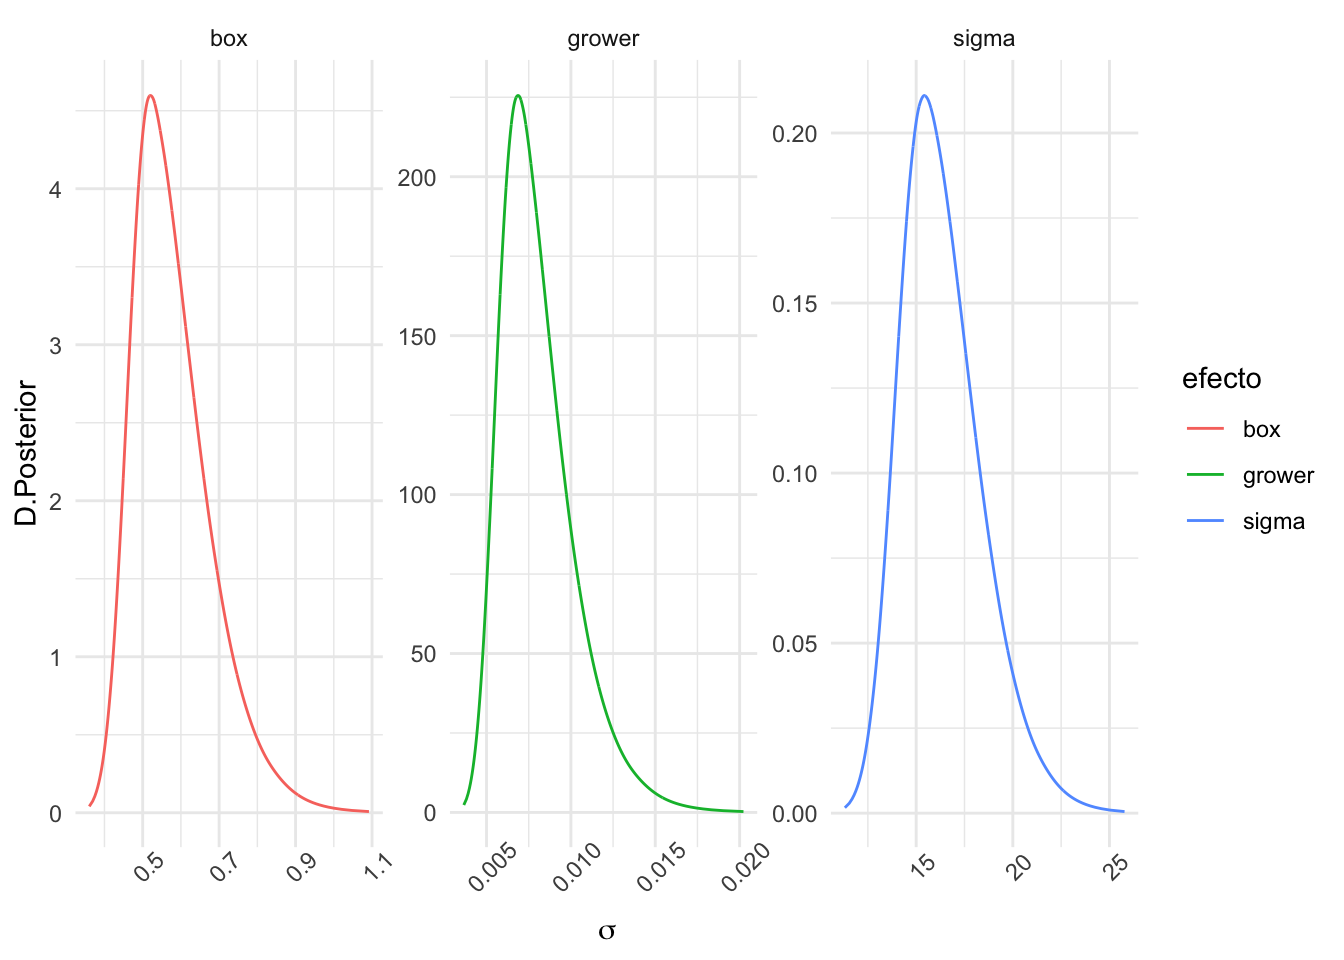
\includegraphics{02-anova_files/figure-latex/brocoli2-1.pdf}
\caption{\label{fig:brocoli2}Distribución posterior de la desviación típica para las tres fuentes de error: datos, caja y cultivador}
\end{figure}

No obstante, antes de tomar una decisión sobre la exclusión de los efectos aleatorios, vamos a hacer una aproximación del porcentaje de varianza explicada por cada una de estas fuentes de variación. Utilizando simulaciones de las distribuciones posteriores de \(\sigma^2, \sigma_{\alpha}^2\) y \(\sigma_{\beta}^2\) vamos a calcular la contribución a la varianza del efecto cultivador, \$ \sigma\emph{\{\alpha\}\textsuperscript{2/(\sigma}2 + \sigma}\{\alpha\}\textsuperscript{2+\sigma\emph{\{\beta\}\^{}2)\$ y la contribución a la varianza del efecto caja, \$ \sigma}\{\beta\}}2/(\sigma\^{}2 + \sigma\emph{\{\alpha\}\^{}2+\sigma}\{\beta\}\^{}2)\$, y calcular con ellas un porcentaje promedio.

\begin{Shaded}
\begin{Highlighting}[]
\NormalTok{n}\OtherTok{=}\DecValTok{1000}
\NormalTok{tau}\OtherTok{=}\FunctionTok{as.data.frame}\NormalTok{(}\FunctionTok{inla.hyperpar.sample}\NormalTok{(n,fit,}\AttributeTok{improve.marginals=}\ConstantTok{TRUE}\NormalTok{))}
\NormalTok{sigma2}\OtherTok{=}\FunctionTok{apply}\NormalTok{(tau,}\DecValTok{2}\NormalTok{,}\ControlFlowTok{function}\NormalTok{(x) }\DecValTok{1}\SpecialCharTok{/}\NormalTok{x)}
\FunctionTok{colnames}\NormalTok{(sigma2)}\OtherTok{=}\FunctionTok{c}\NormalTok{(}\StringTok{"sigma2d"}\NormalTok{,}\StringTok{"sigma2G"}\NormalTok{,}\StringTok{"sigma2B"}\NormalTok{)}
\CommentTok{\# contribución a la varianza de grower}
\NormalTok{cG}\OtherTok{=}\NormalTok{ sigma2[,}\DecValTok{2}\NormalTok{]}\SpecialCharTok{/}\FunctionTok{apply}\NormalTok{(sigma2,}\DecValTok{1}\NormalTok{,sum)}
\CommentTok{\# contribución a la varianza de grower}
\NormalTok{cB}\OtherTok{=}\NormalTok{ sigma2[,}\DecValTok{3}\NormalTok{]}\SpecialCharTok{/}\FunctionTok{apply}\NormalTok{(sigma2,}\DecValTok{1}\NormalTok{,sum)}
\FunctionTok{cat}\NormalTok{(}\FunctionTok{paste}\NormalTok{(}\StringTok{"Contribución media de grower a la varianza:"}\NormalTok{,}\FunctionTok{round}\NormalTok{(}\FunctionTok{mean}\NormalTok{(cG)}\SpecialCharTok{*}\DecValTok{100}\NormalTok{,}\DecValTok{6}\NormalTok{),}\StringTok{"por 100"}\NormalTok{,}\StringTok{"}\SpecialCharTok{\textbackslash{}n}\StringTok{"}\NormalTok{))}
\CommentTok{\#\textgreater{} Contribución media de grower a la varianza: 0.00011 por 100}
\FunctionTok{cat}\NormalTok{(}\FunctionTok{paste}\NormalTok{(}\StringTok{"Contribución media de box a la varianza:"}\NormalTok{,}\FunctionTok{round}\NormalTok{(}\FunctionTok{mean}\NormalTok{(cB)}\SpecialCharTok{*}\DecValTok{100}\NormalTok{,}\DecValTok{6}\NormalTok{),}\StringTok{"por 100"}\NormalTok{))}
\CommentTok{\#\textgreater{} Contribución media de box a la varianza: 0.000132 por 100}
\end{Highlighting}
\end{Shaded}

Ante estos resultados, y dados los valores del DIC (307.1382561) y del WAIC (307.0682172), se justifica la opción de prescindir de los efectos \texttt{grower} y \texttt{box} como efectos aleatorios y ajustar el modelo con un único efecto fijo global.

\begin{Shaded}
\begin{Highlighting}[]
\NormalTok{formula }\OtherTok{=}\NormalTok{ wt }\SpecialCharTok{\textasciitilde{}} \DecValTok{1}
\NormalTok{fit }\OtherTok{=} \FunctionTok{inla}\NormalTok{(formula, }\AttributeTok{family=}\StringTok{"gaussian"}\NormalTok{,}\AttributeTok{data=}\NormalTok{broccoli,}
           \AttributeTok{control.compute =} \FunctionTok{list}\NormalTok{(}\AttributeTok{dic=}\ConstantTok{TRUE}\NormalTok{,}\AttributeTok{waic=}\ConstantTok{TRUE}\NormalTok{))  }
\NormalTok{fit}\SpecialCharTok{$}\NormalTok{summary.fixed}
\CommentTok{\#\textgreater{}                 mean       sd 0.025quant 0.5quant}
\CommentTok{\#\textgreater{} (Intercept) 358.1667 2.771112   352.6996 358.1667}
\CommentTok{\#\textgreater{}             0.975quant mode          kld}
\CommentTok{\#\textgreater{} (Intercept)   363.6337   NA 1.211947e{-}08}
\NormalTok{fit}\SpecialCharTok{$}\NormalTok{summary.hyperpar}
\CommentTok{\#\textgreater{}                                                mean}
\CommentTok{\#\textgreater{} Precision for the Gaussian observations 0.003758278}
\CommentTok{\#\textgreater{}                                                   sd}
\CommentTok{\#\textgreater{} Precision for the Gaussian observations 0.0008870513}
\CommentTok{\#\textgreater{}                                          0.025quant}
\CommentTok{\#\textgreater{} Precision for the Gaussian observations 0.002261799}
\CommentTok{\#\textgreater{}                                            0.5quant}
\CommentTok{\#\textgreater{} Precision for the Gaussian observations 0.003680228}
\CommentTok{\#\textgreater{}                                          0.975quant mode}
\CommentTok{\#\textgreater{} Precision for the Gaussian observations 0.005742648   NA}
\end{Highlighting}
\end{Shaded}

Vemos que la variación en los indicadores DIC (308.0755903) y WAIC (308.0833022) es despreciable para este nuevo modelo.

Inferimos a continuación con las distribuciones posteriores para la media global y la varianza de los datos.

\begin{Shaded}
\begin{Highlighting}[]
\NormalTok{theta.post }\OtherTok{=} \FunctionTok{as.data.frame}\NormalTok{(fit}\SpecialCharTok{$}\NormalTok{marginals.fixed[[}\DecValTok{1}\NormalTok{]])}
\NormalTok{sigma.post}\OtherTok{=}\FunctionTok{as.data.frame}\NormalTok{(}\FunctionTok{inla.tmarginal}\NormalTok{(}\ControlFlowTok{function}\NormalTok{(tau) tau}\SpecialCharTok{\^{}}\NormalTok{(}\SpecialCharTok{{-}}\DecValTok{1}\SpecialCharTok{/}\DecValTok{2}\NormalTok{),}
\NormalTok{  fit}\SpecialCharTok{$}\NormalTok{marginals.hyperpar[[}\DecValTok{1}\NormalTok{]]))}

\NormalTok{posterior}\OtherTok{=}\FunctionTok{rbind}\NormalTok{(theta.post,sigma.post)}
\NormalTok{posterior}\SpecialCharTok{$}\NormalTok{efecto}\OtherTok{=}\FunctionTok{rep}\NormalTok{(}\FunctionTok{c}\NormalTok{(}\StringTok{"theta"}\NormalTok{,}\StringTok{"sigma"}\NormalTok{),}
                     \FunctionTok{c}\NormalTok{(}\FunctionTok{nrow}\NormalTok{(theta.post),}\FunctionTok{nrow}\NormalTok{(sigma.post)))}
\FunctionTok{ggplot}\NormalTok{(posterior,}\FunctionTok{aes}\NormalTok{(}\AttributeTok{x=}\NormalTok{x,}\AttributeTok{y=}\NormalTok{y)) }\SpecialCharTok{+} 
  \FunctionTok{geom\_line}\NormalTok{(}\FunctionTok{aes}\NormalTok{(}\AttributeTok{color=}\NormalTok{efecto)) }\SpecialCharTok{+}
  \FunctionTok{labs}\NormalTok{(}\AttributeTok{x=}\StringTok{""}\NormalTok{,}\AttributeTok{y=}\StringTok{"D.Posterior"}\NormalTok{)}\SpecialCharTok{+}
  \FunctionTok{facet\_wrap}\NormalTok{(}\FunctionTok{vars}\NormalTok{(efecto),}\AttributeTok{scales =} \StringTok{"free"}\NormalTok{)}\SpecialCharTok{+}
  \FunctionTok{theme}\NormalTok{(}\AttributeTok{legend.position =} \StringTok{"none"}\NormalTok{)}
\end{Highlighting}
\end{Shaded}

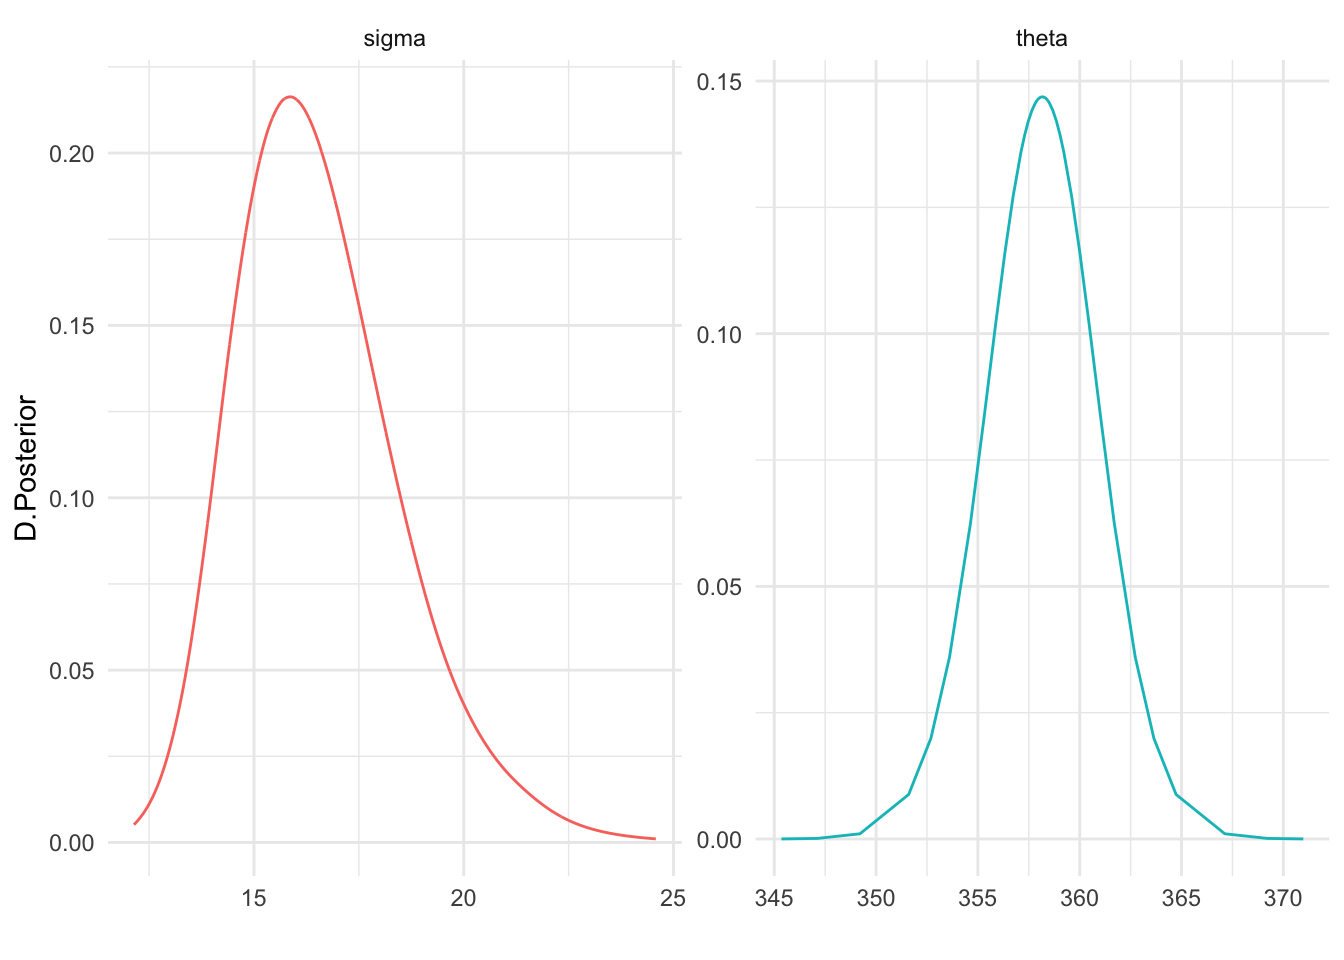
\includegraphics{02-anova_files/figure-latex/unnamed-chunk-25-1.pdf}
Hemos concluido con este análisis, que todos los cultivadores han respetado los protocolos de calidad establecidos para el empaquetado en cajas.

\hypertarget{modelos-mixtos}{%
\section{Modelos mixtos}\label{modelos-mixtos}}

En ocasiones cuando ajustamos un modelo lineal tendremos algunos factores de clasificación que operan como efectos fijos y otros que operan como efectos aleatorios. Estaremos ante \textbf{modelos lineales mixtos}. Siendo estrictos, realmente el modelo con solo efectos aleatorios ya es un modelo mixto, puesto que incluye como efecto fijo una interceptación global.

En un modelo lineal mixto seguimos asumiendo una respuesta normal, \emph{gaussian}, con media igual a un predictor lineal \(\eta=X\beta + Z u\), donde \(X\) es una matriz de diseño con los efectos fijos \(x_1,x_2,...\), y \(Z\) la correspondiente para los efectos aleatorios \(z_1, z_2,...\). Se asume además una varianza desconocida que puede ser distinta para distintos niveles de los predictores, e incluso contener correlaciones entre niveles distintos, y que en general se suele expresar a través de una matriz de covarianzas \(\Sigma\), \((y|\eta,\Sigma) \sim N(\eta,\Sigma)\).

En INLA la fórmula de predicción de una respuesta \(y\) a partir de un conjunto de efectos fijos x1,x2,\ldots, y un conjunto de efectos aleatorios z1,z2,\ldots{} se especifica como:

\begin{Shaded}
\begin{Highlighting}[]
\NormalTok{formula }\OtherTok{=}\NormalTok{ y }\SpecialCharTok{\textasciitilde{}} \DecValTok{1} \SpecialCharTok{+}\NormalTok{ x1 }\SpecialCharTok{+}\NormalTok{ x2  }\SpecialCharTok{+} \FunctionTok{f}\NormalTok{(z1, }\AttributeTok{model=}\StringTok{""}\NormalTok{) }\SpecialCharTok{+} \FunctionTok{f}\NormalTok{(z2,}\AttributeTok{model=}\StringTok{""}\NormalTok{) }
\end{Highlighting}
\end{Shaded}

De nuevo mencionar que la opción más habitual para los efectos aleatorios en un modelo lineal es \texttt{model="iid"}.

\hypertarget{datos-longitudinales-con-pendientes-iguales}{%
\subsection{Datos longitudinales con pendientes iguales}\label{datos-longitudinales-con-pendientes-iguales}}

Veamos cómo resolver las inferencias a través de un ejemplo disponible en \href{https://www.r-bloggers.com/2019/09/bayesian-linear-mixed-models-random-intercepts-slopes-and-missing-data/}{R-bloggers}, proporcionado por \href{https://curran.web.unc.edu/}{Patrick Curran} y descargable desde \href{https://github.com/MultiLevelAnalysis/Datasets-third-edition-Multilevel-book/blob/master/chapter\%205/Curran/CurranLong.sav}{Github}. Se refieren estos datos, a un estudio con 405 niños en los dos primeros años de la escuela infantil, medidos a lo largo de cuatro instantes equidistantes (no medidos todos en todos los sujetos) para registrar su progreso en lectura y en comportamiento antisocial. Nos centramos aquí exclusivamente en intentar predecir los progresos en lectura (variable \texttt{read}) para cada sujeto (identificado como \texttt{id}) a lo largo de los 4 instantes de medición (\texttt{occasion}).

Cargamos los datos, prescindimos de los que tienen valores faltantes, y los inspeccionamos en la Figura \ref{fig:curran1}.

\begin{Shaded}
\begin{Highlighting}[]
\NormalTok{url}\OtherTok{=}\StringTok{"https://raw.githubusercontent.com/BayesModel/data/main/curran\_dat.csv"}
\NormalTok{curran\_dat}\OtherTok{=}\FunctionTok{read.csv}\NormalTok{(url) }\SpecialCharTok{\%\textgreater{}\%}
  \FunctionTok{select}\NormalTok{(id, occasion, read) }\SpecialCharTok{\%\textgreater{}\%}
  \FunctionTok{filter}\NormalTok{(}\FunctionTok{complete.cases}\NormalTok{(.))}
\CommentTok{\# el identificador de cada sujeto lo convertimos a factor}
\NormalTok{curran\_dat}\SpecialCharTok{$}\NormalTok{id}\OtherTok{=}\FunctionTok{as.factor}\NormalTok{(curran\_dat}\SpecialCharTok{$}\NormalTok{id)}
\NormalTok{curran\_dat}\SpecialCharTok{$}\NormalTok{occasion}\OtherTok{=}\FunctionTok{as.double}\NormalTok{(curran\_dat}\SpecialCharTok{$}\NormalTok{occasion)}
\CommentTok{\# Relaciones}
\NormalTok{g1}\OtherTok{=}\FunctionTok{ggplot}\NormalTok{(curran\_dat, }\FunctionTok{aes}\NormalTok{(}\AttributeTok{x=}\FunctionTok{as.factor}\NormalTok{(occasion),}\AttributeTok{y=}\NormalTok{read))}\SpecialCharTok{+}
  \FunctionTok{geom\_boxplot}\NormalTok{()}
\NormalTok{g2}\OtherTok{=}\FunctionTok{ggplot}\NormalTok{(curran\_dat, }\FunctionTok{aes}\NormalTok{(}\AttributeTok{x=}\NormalTok{occasion,}\AttributeTok{y=}\NormalTok{read))}\SpecialCharTok{+}
  \FunctionTok{geom\_line}\NormalTok{(}\FunctionTok{aes}\NormalTok{(}\AttributeTok{group=}\NormalTok{id),}\AttributeTok{color=}\StringTok{"grey"}\NormalTok{,}\AttributeTok{size=}\FloatTok{0.4}\NormalTok{)}
\FunctionTok{grid.arrange}\NormalTok{(g1,g2,}\AttributeTok{ncol=}\DecValTok{2}\NormalTok{)}
\end{Highlighting}
\end{Shaded}

\begin{figure}
\centering
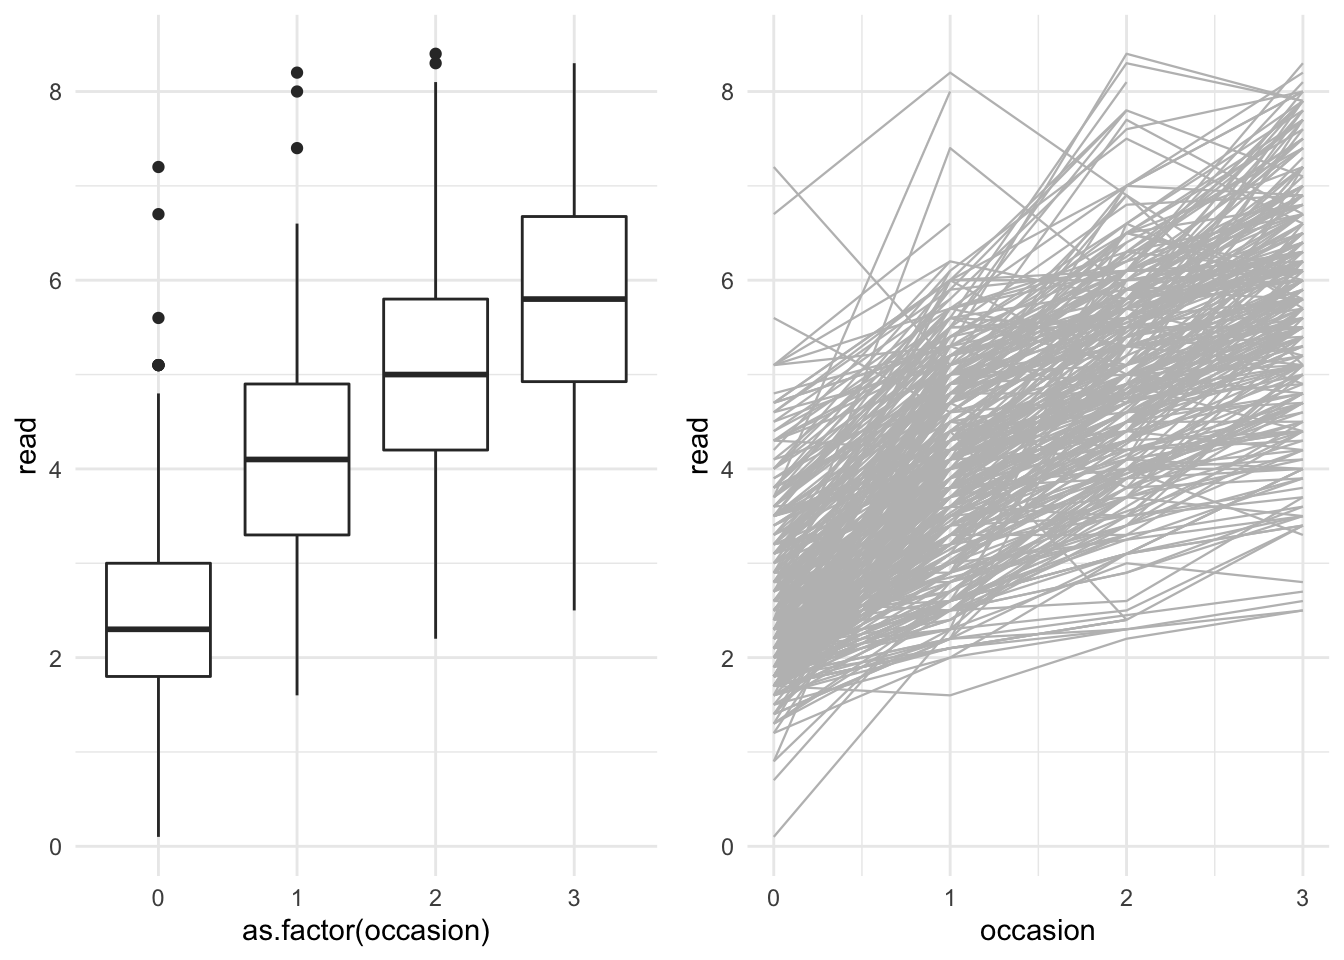
\includegraphics{02-anova_files/figure-latex/curran1-1.pdf}
\caption{\label{fig:curran1}Descripción de la BD CurranLong sobre desarrollo de las habilidades lectoras en niños.}
\end{figure}

Como base vamos a asumir normalidad en la respuesta de un sujeto \(i\) en un instante \(j\), y plantear un modelo lineal para obtener nuestras conclusiones.
\[( y_{ij}|\mu_{ij},\sigma^2 ) \sim N(\mu_{ij},\sigma^2);  \ i=1,...,450; j=1,2,3,4\]

A la vista de la Figura \ref{fig:curran1} podríamos considerar el tiempo afecta de modo positivo y lineal sobre las habilidades lectoras (a más tiempo, mejores habilidades), lo que convierte a la variable \texttt{occasion} en una covariable numérica (efecto fijo): nos interesará cuantificar cómo afecta el tiempo a la capacidad lectora.

Sin embargo, también en el gráfico apreciamos que cada sujeto arranca de un inicio diferente, o lo que es lo mismo, su recta de predicción tiene una interceptación distinta. Puesto que no nos interesa comparar los individuos, planteamos incorporar un efecto aleatorio del sujeto (variable \texttt{id}). Estamos pues, hablando de predecir la habilidad lectora de un sujeto \(i\) en un instante \(t_{ij}=j\) con:

\[\mu_{ij}=\theta + \alpha_i + \beta \cdot t_{ij} \]
con
\begin{eqnarray*}
\text{Nivel II} && \\
\theta &\sim & N(0,100) \\
\beta &\sim& N(0,100) \\
\alpha_i &\sim& N(0,\sigma_{\alpha}^2) \\
\tau=1/\sigma^2 &\sim& Ga(0.001,0.001) \\
\text{Nivel III} && \\
\tau_{\alpha}=1/\sigma_{\alpha}^2 &\sim& Ga(0.001,0.001) 
\end{eqnarray*}

La varianza \(\sigma_{\alpha}^2\) representa la variabilidad existente entre las distintas interceptaciones o niveles cognitivos de los sujetos en el inicio del estudio.

En la Figura \ref{fig:curran4} se muestran las distribuciones posteriores obtenidas sobre efectos fijos y varianzas.

\begin{Shaded}
\begin{Highlighting}[]
\NormalTok{prec.prior}\OtherTok{=}\FunctionTok{list}\NormalTok{(}\AttributeTok{prec=}\FunctionTok{list}\NormalTok{(}\AttributeTok{param=}\FunctionTok{c}\NormalTok{(}\FloatTok{0.001}\NormalTok{,}\FloatTok{0.001}\NormalTok{)))}
\NormalTok{formula}\OtherTok{=}\NormalTok{ read }\SpecialCharTok{\textasciitilde{}}\NormalTok{ occasion }\SpecialCharTok{+} \FunctionTok{f}\NormalTok{(id,}\AttributeTok{model=}\StringTok{"iid"}\NormalTok{,}\AttributeTok{hyper =}\NormalTok{ prec.prior) }
\NormalTok{fit}\OtherTok{=}\FunctionTok{inla}\NormalTok{(formula,}\AttributeTok{family=}\StringTok{"gaussian"}\NormalTok{,}\AttributeTok{data=}\NormalTok{curran\_dat,}
          \AttributeTok{control.family=}\FunctionTok{list}\NormalTok{(}\AttributeTok{hyper=}\NormalTok{prec.prior))}
\NormalTok{fit}\SpecialCharTok{$}\NormalTok{summary.fixed}
\CommentTok{\#\textgreater{}                 mean         sd 0.025quant 0.5quant}
\CommentTok{\#\textgreater{} (Intercept) 2.703751 0.05266776   2.600408 2.703757}
\CommentTok{\#\textgreater{} occasion    1.101333 0.01760845   1.066782 1.101336}
\CommentTok{\#\textgreater{}             0.975quant mode          kld}
\CommentTok{\#\textgreater{} (Intercept)   2.807060   NA 1.184714e{-}11}
\CommentTok{\#\textgreater{} occasion      1.135862   NA 5.550080e{-}12}
\NormalTok{fit}\SpecialCharTok{$}\NormalTok{summary.hyperpar}
\CommentTok{\#\textgreater{}                                             mean        sd}
\CommentTok{\#\textgreater{} Precision for the Gaussian observations 2.169523 0.1013917}
\CommentTok{\#\textgreater{} Precision for id                        1.286183 0.1093176}
\CommentTok{\#\textgreater{}                                         0.025quant 0.5quant}
\CommentTok{\#\textgreater{} Precision for the Gaussian observations   1.975790 2.167497}
\CommentTok{\#\textgreater{} Precision for id                          1.083454 1.281901}
\CommentTok{\#\textgreater{}                                         0.975quant mode}
\CommentTok{\#\textgreater{} Precision for the Gaussian observations   2.375188   NA}
\CommentTok{\#\textgreater{} Precision for id                          1.513859   NA}

\CommentTok{\# Agrupamos todas las distribuciones posteriores}
\NormalTok{nfixed}\OtherTok{=}\FunctionTok{length}\NormalTok{(}\FunctionTok{names}\NormalTok{(fit}\SpecialCharTok{$}\NormalTok{marginals.fixed))}
\NormalTok{nhyp}\OtherTok{=}\FunctionTok{length}\NormalTok{(}\FunctionTok{names}\NormalTok{(fit}\SpecialCharTok{$}\NormalTok{marginals.hyperpar))}
\NormalTok{res}\OtherTok{=}\ConstantTok{NULL}
\ControlFlowTok{for}\NormalTok{(i }\ControlFlowTok{in} \DecValTok{1}\SpecialCharTok{:}\NormalTok{nfixed)\{}
\NormalTok{res}\OtherTok{=}\FunctionTok{rbind}\NormalTok{(res,}\FunctionTok{data.frame}\NormalTok{(fit}\SpecialCharTok{$}\NormalTok{marginals.fixed[[i]],}
                         \AttributeTok{id=}\FunctionTok{names}\NormalTok{(fit}\SpecialCharTok{$}\NormalTok{marginals.fixed)[i],}
                          \AttributeTok{tipo=}\StringTok{"fixed"}\NormalTok{))}
\NormalTok{\}}
\ControlFlowTok{for}\NormalTok{(j }\ControlFlowTok{in} \DecValTok{1}\SpecialCharTok{:}\NormalTok{nhyp)\{}
\NormalTok{    res}\OtherTok{=}\FunctionTok{rbind}\NormalTok{(res,}\FunctionTok{data.frame}\NormalTok{(}
    \FunctionTok{inla.tmarginal}\NormalTok{(}\ControlFlowTok{function}\NormalTok{(tau) tau}\SpecialCharTok{\^{}}\NormalTok{(}\SpecialCharTok{{-}}\DecValTok{1}\SpecialCharTok{/}\DecValTok{2}\NormalTok{),fit}\SpecialCharTok{$}\NormalTok{marginals.hyperpar[[j]]),}
                         \AttributeTok{id=}\FunctionTok{str\_sub}\NormalTok{(}\FunctionTok{names}\NormalTok{(fit}\SpecialCharTok{$}\NormalTok{marginals.hyperpar)[j], }\AttributeTok{start =}\DecValTok{15}\NormalTok{),}
                          \AttributeTok{tipo=}\StringTok{"sigma"}\NormalTok{))}
\NormalTok{\}}
\FunctionTok{ggplot}\NormalTok{(res,}\FunctionTok{aes}\NormalTok{(}\AttributeTok{x=}\NormalTok{x,}\AttributeTok{y=}\NormalTok{y))}\SpecialCharTok{+}
  \FunctionTok{geom\_line}\NormalTok{(}\FunctionTok{aes}\NormalTok{(}\AttributeTok{color=}\NormalTok{id))}\SpecialCharTok{+}
  \FunctionTok{facet\_wrap}\NormalTok{(}\FunctionTok{vars}\NormalTok{(tipo),}\AttributeTok{scales=}\StringTok{"free"}\NormalTok{)}\SpecialCharTok{+}
  \FunctionTok{theme}\NormalTok{(}\AttributeTok{legend.position=}\StringTok{"top"}\NormalTok{,}
        \AttributeTok{legend.title=}\FunctionTok{element\_blank}\NormalTok{(),}
        \AttributeTok{legend.text =} \FunctionTok{element\_text}\NormalTok{(}\AttributeTok{size=}\DecValTok{5}\NormalTok{))}
\end{Highlighting}
\end{Shaded}

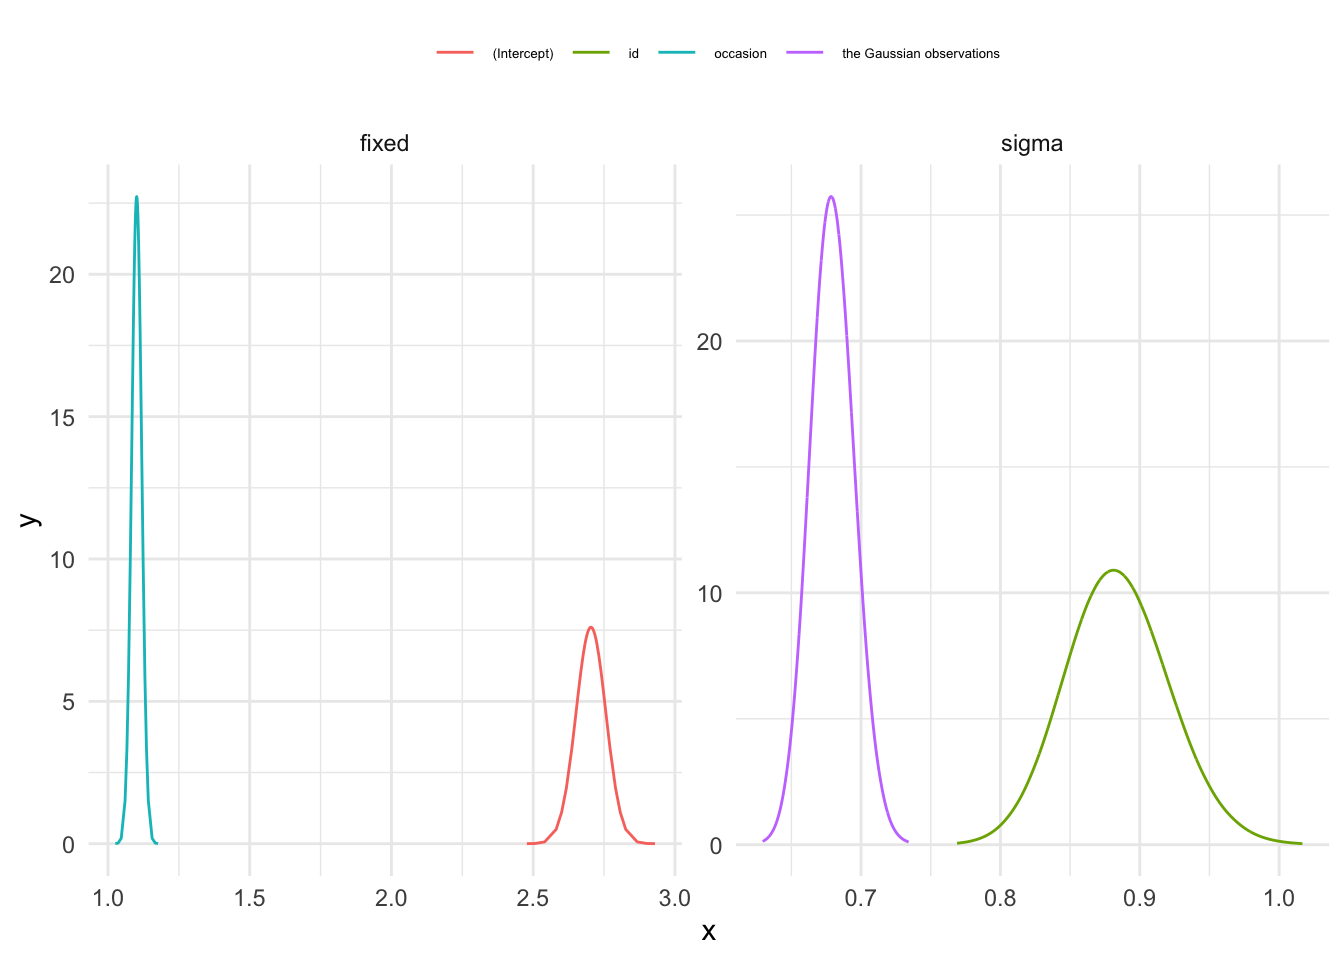
\includegraphics{02-anova_files/figure-latex/curran4-1.pdf}
\#\#\# Datos longitudinales con pendientes distintas

Belenky et al.~(2003) describen un estudio de los tiempos de reacción en pacientes a los que se ha privado de sueño durante 10 días; cada día se ha ido registrando la respuesta para cada uno de los 18 sujetos en el estudio. Los datos están disponibles como \texttt{sleepstudy} en la librería \texttt{lme4} y tienen como variables el tiempo medio de reacción en microsegundos (\texttt{Reaction}), el número de días con privación de sueño (\texttt{Days}) y un id para cada sujeto (\texttt{Subject}). Los tiempos de reacción se transforman a segundos para tener mayor estabilidad. Aun así, en la Figura \ref{fig:sleep1} se aprecia que el número de días de falta de sueño afecta de modo distinto a cada sujeto.

\begin{Shaded}
\begin{Highlighting}[]
\FunctionTok{data}\NormalTok{(sleepstudy,}\AttributeTok{package=}\StringTok{"lme4"}\NormalTok{)}
\NormalTok{sleepstudy}\SpecialCharTok{$}\NormalTok{Reaction }\OtherTok{\textless{}{-}}\NormalTok{ sleepstudy}\SpecialCharTok{$}\NormalTok{Reaction }\SpecialCharTok{/} \DecValTok{1000}
\FunctionTok{ggplot}\NormalTok{(sleepstudy,}\FunctionTok{aes}\NormalTok{(}\AttributeTok{x=}\NormalTok{Days,}\AttributeTok{y=}\NormalTok{Reaction))}\SpecialCharTok{+}
  \FunctionTok{geom\_point}\NormalTok{(}\AttributeTok{size=}\FloatTok{0.5}\NormalTok{)}\SpecialCharTok{+}
  \FunctionTok{geom\_smooth}\NormalTok{(}\AttributeTok{method=}\StringTok{"lm"}\NormalTok{,}\AttributeTok{color=}\StringTok{"blue"}\NormalTok{,}\AttributeTok{size=}\FloatTok{0.5}\NormalTok{)}\SpecialCharTok{+}
  \FunctionTok{facet\_wrap}\NormalTok{(}\FunctionTok{vars}\NormalTok{(Subject),}\AttributeTok{ncol=}\DecValTok{6}\NormalTok{)}\SpecialCharTok{+}
  \FunctionTok{theme}\NormalTok{(}\AttributeTok{axis.text.x =} \FunctionTok{element\_text}\NormalTok{(}\AttributeTok{size=}\DecValTok{5}\NormalTok{),}
        \AttributeTok{axis.text.y =} \FunctionTok{element\_text}\NormalTok{(}\AttributeTok{size=}\DecValTok{5}\NormalTok{))}
\CommentTok{\#\textgreater{} \textasciigrave{}geom\_smooth()\textasciigrave{} using formula \textquotesingle{}y \textasciitilde{} x\textquotesingle{}}
\end{Highlighting}
\end{Shaded}

\begin{figure}
\centering
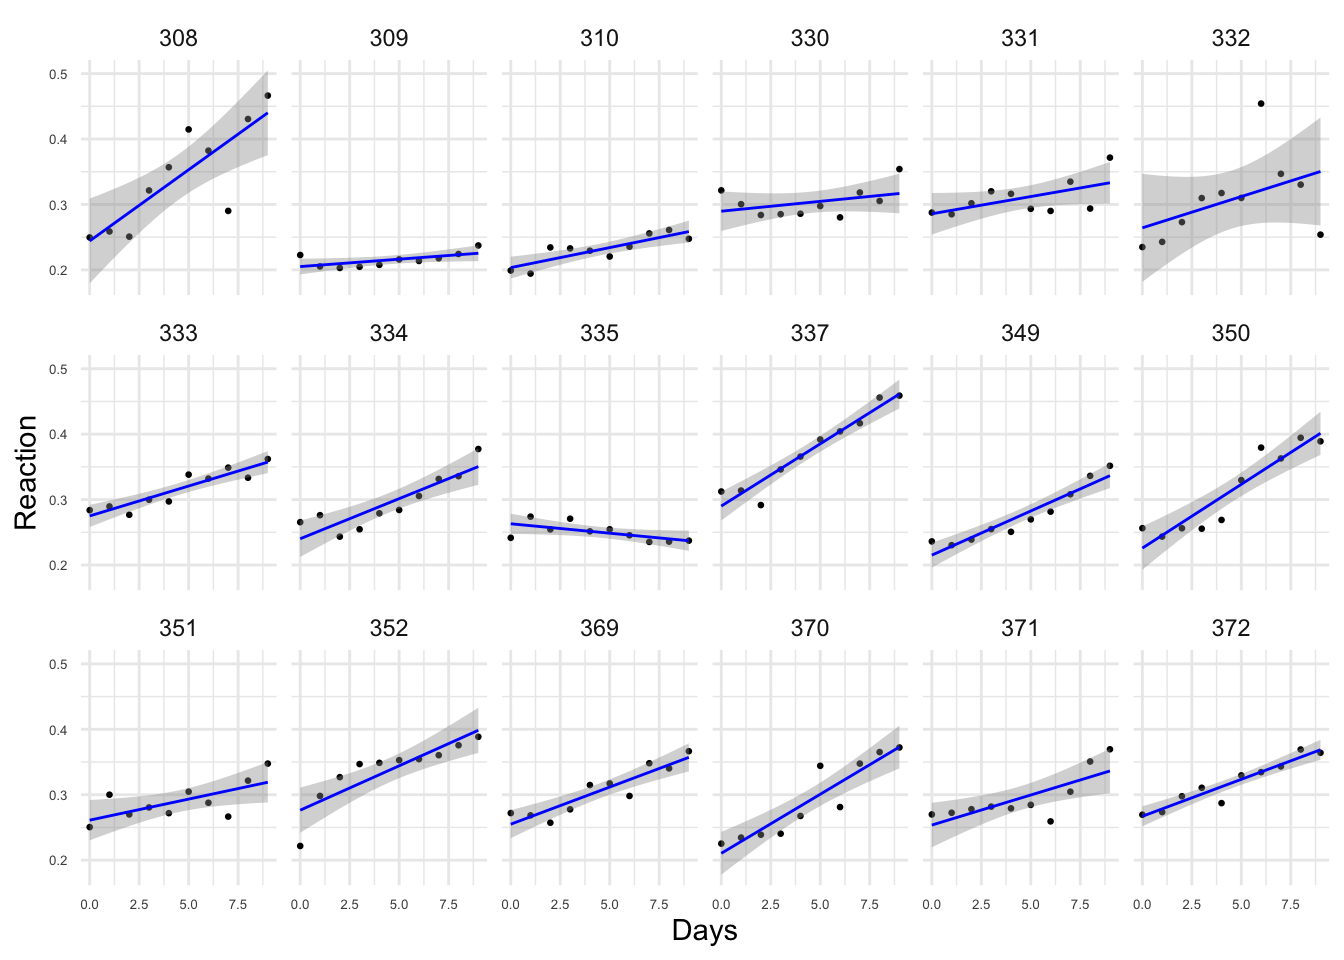
\includegraphics{02-anova_files/figure-latex/sleep1-1.pdf}
\caption{\label{fig:sleep1}Tiempos de reacción en función del número de días con falta de sueño (sleepstudy) para los 18 sujetos en el estudio}
\end{figure}

Un modelo razonable para estos datos es un modelo lineal que relacione los tiempos de reacción con los días, pero que tenga interceptaciones y pendientes diferentes para cada sujeto. El efecto sujeto entraría en el modelo como un efecto aleatorio para relacionar todos los datos del mismo sujeto sin perder la asunción de independencia entre las observaciones de sujetos distintos. Si llamamos \(y=Reaction\) a la respuesta, estaríamos planteando el siguiente modelo:

\[ y_{ij}|\mu_{ij},\sigma^2 \sim N(\mu,\sigma^2), i=1,...,18; j=1, ...,10\]

con

\[\mu_{ij}=\theta + \alpha_i + \beta \cdot x_{ij} + \gamma_{ij}\]

donde el predictor \(x\) es la variable \texttt{Days}, \((\theta,\beta)\) se tratarían como efectos fijos con a prioris difusas ante falta de información, y \((\alpha_i,\gamma_{ij})\) como efectos aleatorios, con normales centradas en cero y una varianza desconocida a la que habría que asignar así mismo, una distribución a priori. El modelo jerárquico que surge es pues:

\begin{eqnarray*}
\text{Nivel I} && \\
y_{ij}|\mu_{ij},\sigma^2 &\sim& N(\mu,\sigma^2), i=1,...,18; j=1, ...,10 \\
\text{Nivel II} && \\
\theta &\sim & N(0,1000) \\
\beta &\sim& N(0,1000) \\
\alpha_i &\sim& N(0,\sigma_{\alpha}^2) \\
\gamma_{ij} &\sim & N(0,\sigma_{\gamma})^2 \\
\tau=1/\sigma^2 &\sim& Ga(0.001,0.001)\\
\text{Nivel III} && \\
\tau_{\alpha}=1/\sigma_{\alpha}^2 &\sim& Ga(0.001,0.001) \\
\tau_{\gamma}=1/\sigma_{\alpha}^2 &\sim& Ga(0.001,0.001) \end{eqnarray*}

En INLA modelizamos esta propuesta utilizando como predictores;

\begin{itemize}
\tightlist
\item
  la covariable para generar una interceptación `media' (efecto fijo),
\item
  el efecto aleatorio de cada sujeto para generar interceptaciones distintas,
\item
  la interacción entre la covariable y el efecto aleatorio, a través de la matriz de diseño que hemos de construir específicamente, y definir en paralelo un índice de la misma dimensión de los datos, para aplicarla. En la interacción la primera variable define el número de grupos y la segunda el valor de la covariable.
\end{itemize}

\begin{Shaded}
\begin{Highlighting}[]
\NormalTok{prec.prior}\OtherTok{=}\FunctionTok{list}\NormalTok{(}\AttributeTok{prec=}\FunctionTok{list}\NormalTok{(}\AttributeTok{param=}\FunctionTok{c}\NormalTok{(}\FloatTok{0.001}\NormalTok{,}\FloatTok{0.001}\NormalTok{)))}
\CommentTok{\# matriz de diseño para la interacción}
\NormalTok{Z }\OtherTok{\textless{}{-}} \FunctionTok{as}\NormalTok{(}\FunctionTok{model.matrix}\NormalTok{( }\SpecialCharTok{\textasciitilde{}} \DecValTok{0} \SpecialCharTok{+}\NormalTok{ Subject}\SpecialCharTok{:}\NormalTok{Days, }\AttributeTok{data =}\NormalTok{ sleepstudy), }\StringTok{"Matrix"}\NormalTok{)}
\CommentTok{\# índice para aplicar la matriz de diseño}
\NormalTok{DayR}\OtherTok{=}\DecValTok{1}\SpecialCharTok{:}\FunctionTok{nrow}\NormalTok{(sleepstudy)}
\NormalTok{formula}\OtherTok{=}\NormalTok{ Reaction }\SpecialCharTok{\textasciitilde{}}\NormalTok{ Days }\SpecialCharTok{+} \FunctionTok{f}\NormalTok{(Subject,}\AttributeTok{model=}\StringTok{"iid"}\NormalTok{,}\AttributeTok{hyper=}\NormalTok{prec.prior)}\SpecialCharTok{+}
  \FunctionTok{f}\NormalTok{(DayR,}\AttributeTok{model=}\StringTok{"z"}\NormalTok{,}\AttributeTok{Z=}\NormalTok{Z,}\AttributeTok{hyper =}\NormalTok{ prec.prior) }
\NormalTok{fit}\OtherTok{=}\FunctionTok{inla}\NormalTok{(formula,}\AttributeTok{family=}\StringTok{"gaussian"}\NormalTok{,}\AttributeTok{data=}\NormalTok{sleepstudy,}
         \AttributeTok{control.compute=}\FunctionTok{list}\NormalTok{(}\AttributeTok{config=}\ConstantTok{TRUE}\NormalTok{))}
\CommentTok{\#\textgreater{} Warning in inla.model.properties.generic(inla.trim.family(model), mm[names(mm) == : Model \textquotesingle{}z\textquotesingle{} in section \textquotesingle{}latent\textquotesingle{} is marked as \textquotesingle{}experimental\textquotesingle{}; changes may appear at any time.}
\CommentTok{\#\textgreater{}   Use this model with extra care!!! Further warnings are disabled.}
\CommentTok{\#\textgreater{} as(\textless{}dgCMatrix\textgreater{}, "dgTMatrix") is deprecated since Matrix 1.5{-}0; do as(., "TsparseMatrix") instead}
\end{Highlighting}
\end{Shaded}

Obtenemos en consecuencia, efectos fijos e hiperparámetros, cuyas inferencias posteriores se resumen con:

\begin{Shaded}
\begin{Highlighting}[]
\FunctionTok{round}\NormalTok{(fit}\SpecialCharTok{$}\NormalTok{summary.fixed,}\DecValTok{3}\NormalTok{)}
\CommentTok{\#\textgreater{}              mean    sd 0.025quant 0.5quant 0.975quant mode}
\CommentTok{\#\textgreater{} (Intercept) 0.251 0.008      0.236    0.251      0.267   NA}
\CommentTok{\#\textgreater{} Days        0.010 0.003      0.004    0.010      0.017   NA}
\CommentTok{\#\textgreater{}             kld}
\CommentTok{\#\textgreater{} (Intercept)   0}
\CommentTok{\#\textgreater{} Days          0}
\FunctionTok{round}\NormalTok{(fit}\SpecialCharTok{$}\NormalTok{summary.hyperpar,}\DecValTok{3}\NormalTok{)}
\CommentTok{\#\textgreater{}                                             mean       sd}
\CommentTok{\#\textgreater{} Precision for the Gaussian observations 1566.713  182.872}
\CommentTok{\#\textgreater{} Precision for Subject                   1314.756  571.894}
\CommentTok{\#\textgreater{} Precision for DayR                      6067.459 2128.986}
\CommentTok{\#\textgreater{}                                         0.025quant 0.5quant}
\CommentTok{\#\textgreater{} Precision for the Gaussian observations   1231.363 1558.539}
\CommentTok{\#\textgreater{} Precision for Subject                      520.889 1209.117}
\CommentTok{\#\textgreater{} Precision for DayR                        2819.871 5762.946}
\CommentTok{\#\textgreater{}                                         0.975quant mode}
\CommentTok{\#\textgreater{} Precision for the Gaussian observations   1950.856   NA}
\CommentTok{\#\textgreater{} Precision for Subject                     2728.351   NA}
\CommentTok{\#\textgreater{} Precision for DayR                       11105.474   NA}
\end{Highlighting}
\end{Shaded}

Y los efectos aleatorios:

\begin{Shaded}
\begin{Highlighting}[]
\FunctionTok{names}\NormalTok{(fit}\SpecialCharTok{$}\NormalTok{marginals.random)}
\CommentTok{\#\textgreater{} [1] "Subject" "DayR"}
\FunctionTok{head}\NormalTok{(fit}\SpecialCharTok{$}\NormalTok{summary.random}\SpecialCharTok{$}\NormalTok{Subject)}
\CommentTok{\#\textgreater{}    ID         mean         sd    0.025quant     0.5quant}
\CommentTok{\#\textgreater{} 1 308 {-}0.003768873 0.01446456 {-}0.0322860523 {-}0.003748488}
\CommentTok{\#\textgreater{} 2 309 {-}0.037615026 0.01485947 {-}0.0674457611 {-}0.037392853}
\CommentTok{\#\textgreater{} 3 310 {-}0.038204929 0.01487073 {-}0.0680612695 {-}0.037981229}
\CommentTok{\#\textgreater{} 4 330  0.028706038 0.01469943  0.0002843602  0.028533780}
\CommentTok{\#\textgreater{} 5 331  0.025993687 0.01465102 {-}0.0023753055  0.025835697}
\CommentTok{\#\textgreater{} 6 332  0.009899260 0.01447477 {-}0.0184010587  0.009836417}
\CommentTok{\#\textgreater{}     0.975quant mode          kld}
\CommentTok{\#\textgreater{} 1  0.024632758   NA 5.824804e{-}09}
\CommentTok{\#\textgreater{} 2 {-}0.009029249   NA 2.027815e{-}08}
\CommentTok{\#\textgreater{} 3 {-}0.009601978   NA 2.046358e{-}08}
\CommentTok{\#\textgreater{} 4  0.058095611   NA 1.427011e{-}08}
\CommentTok{\#\textgreater{} 5  0.055251271   NA 1.290458e{-}08}
\CommentTok{\#\textgreater{} 6  0.038554384   NA 6.836930e{-}09}
\FunctionTok{head}\NormalTok{(fit}\SpecialCharTok{$}\NormalTok{summary.random}\SpecialCharTok{$}\NormalTok{DayR)}
\CommentTok{\#\textgreater{}   ID         mean          sd   0.025quant     0.5quant}
\CommentTok{\#\textgreater{} 1  1 6.924238e{-}06 0.001501481 {-}0.002937713 6.924441e{-}06}
\CommentTok{\#\textgreater{} 2  2 1.056645e{-}02 0.004274277  0.002188708 1.055373e{-}02}
\CommentTok{\#\textgreater{} 3  3 2.106572e{-}02 0.008121904  0.005144073 2.103765e{-}02}
\CommentTok{\#\textgreater{} 4  4 3.184263e{-}02 0.012056271  0.008205544 3.180030e{-}02}
\CommentTok{\#\textgreater{} 5  5 4.249502e{-}02 0.016013237  0.011099076 4.243831e{-}02}
\CommentTok{\#\textgreater{} 6  6 5.322669e{-}02 0.019979621  0.014052978 5.315583e{-}02}
\CommentTok{\#\textgreater{}   0.975quant mode          kld}
\CommentTok{\#\textgreater{} 1 0.00295156   NA 5.527465e{-}11}
\CommentTok{\#\textgreater{} 2 0.01901744   NA 7.952215e{-}09}
\CommentTok{\#\textgreater{} 3 0.03714924   NA 1.020996e{-}08}
\CommentTok{\#\textgreater{} 4 0.05572396   NA 1.066195e{-}08}
\CommentTok{\#\textgreater{} 5 0.07421819   NA 1.083096e{-}08}
\CommentTok{\#\textgreater{} 6 0.09280922   NA 1.090800e{-}08}
\end{Highlighting}
\end{Shaded}

En la Figura \ref{fig:sleep2} mostramos los datos y también los valores ajustados para las rectas, en términos de las interceptaciones y pendientes medias de las correspondientes distribuciones posteriores, además de la banda de estimación que construimos con los correspondientes percentiles de las posterioris.

\begin{Shaded}
\begin{Highlighting}[]
\NormalTok{sleepstudy.pred }\OtherTok{=}\NormalTok{ sleepstudy }\SpecialCharTok{\%\textgreater{}\%}
  \FunctionTok{mutate}\NormalTok{(}\AttributeTok{fitted=}\NormalTok{fit}\SpecialCharTok{$}\NormalTok{summary.fitted.values}\SpecialCharTok{$}\NormalTok{mean,}
         \AttributeTok{rc.low=}\NormalTok{fit}\SpecialCharTok{$}\NormalTok{summary.fitted.values}\SpecialCharTok{$}\StringTok{"0.025quant"}\NormalTok{,}
         \AttributeTok{rc.up=}\NormalTok{fit}\SpecialCharTok{$}\NormalTok{summary.fitted.values}\SpecialCharTok{$}\StringTok{"0.975quant"}\NormalTok{) }

\FunctionTok{ggplot}\NormalTok{(sleepstudy.pred,}\FunctionTok{aes}\NormalTok{(}\AttributeTok{x=}\NormalTok{Days,}\AttributeTok{y=}\NormalTok{Reaction))}\SpecialCharTok{+}
  \FunctionTok{geom\_point}\NormalTok{(}\AttributeTok{size=}\FloatTok{0.5}\NormalTok{)}\SpecialCharTok{+}
  \FunctionTok{geom\_line}\NormalTok{(}\FunctionTok{aes}\NormalTok{(}\AttributeTok{y=}\NormalTok{fitted),}\AttributeTok{color=}\StringTok{"blue"}\NormalTok{)}\SpecialCharTok{+}
  \FunctionTok{geom\_line}\NormalTok{(}\FunctionTok{aes}\NormalTok{(}\AttributeTok{y=}\NormalTok{ rc.low),}\AttributeTok{color=}\StringTok{"skyblue"}\NormalTok{)}\SpecialCharTok{+}
  \FunctionTok{geom\_line}\NormalTok{(}\FunctionTok{aes}\NormalTok{(}\AttributeTok{y=}\NormalTok{rc.up),}\AttributeTok{color=}\StringTok{"skyblue"}\NormalTok{)}\SpecialCharTok{+}
  \FunctionTok{facet\_wrap}\NormalTok{(}\FunctionTok{vars}\NormalTok{(Subject),}\AttributeTok{ncol=}\DecValTok{6}\NormalTok{)}\SpecialCharTok{+}
  \FunctionTok{theme}\NormalTok{(}\AttributeTok{axis.text.x =} \FunctionTok{element\_text}\NormalTok{(}\AttributeTok{size=}\DecValTok{5}\NormalTok{),}
        \AttributeTok{axis.text.y =} \FunctionTok{element\_text}\NormalTok{(}\AttributeTok{size=}\DecValTok{5}\NormalTok{))}
\end{Highlighting}
\end{Shaded}

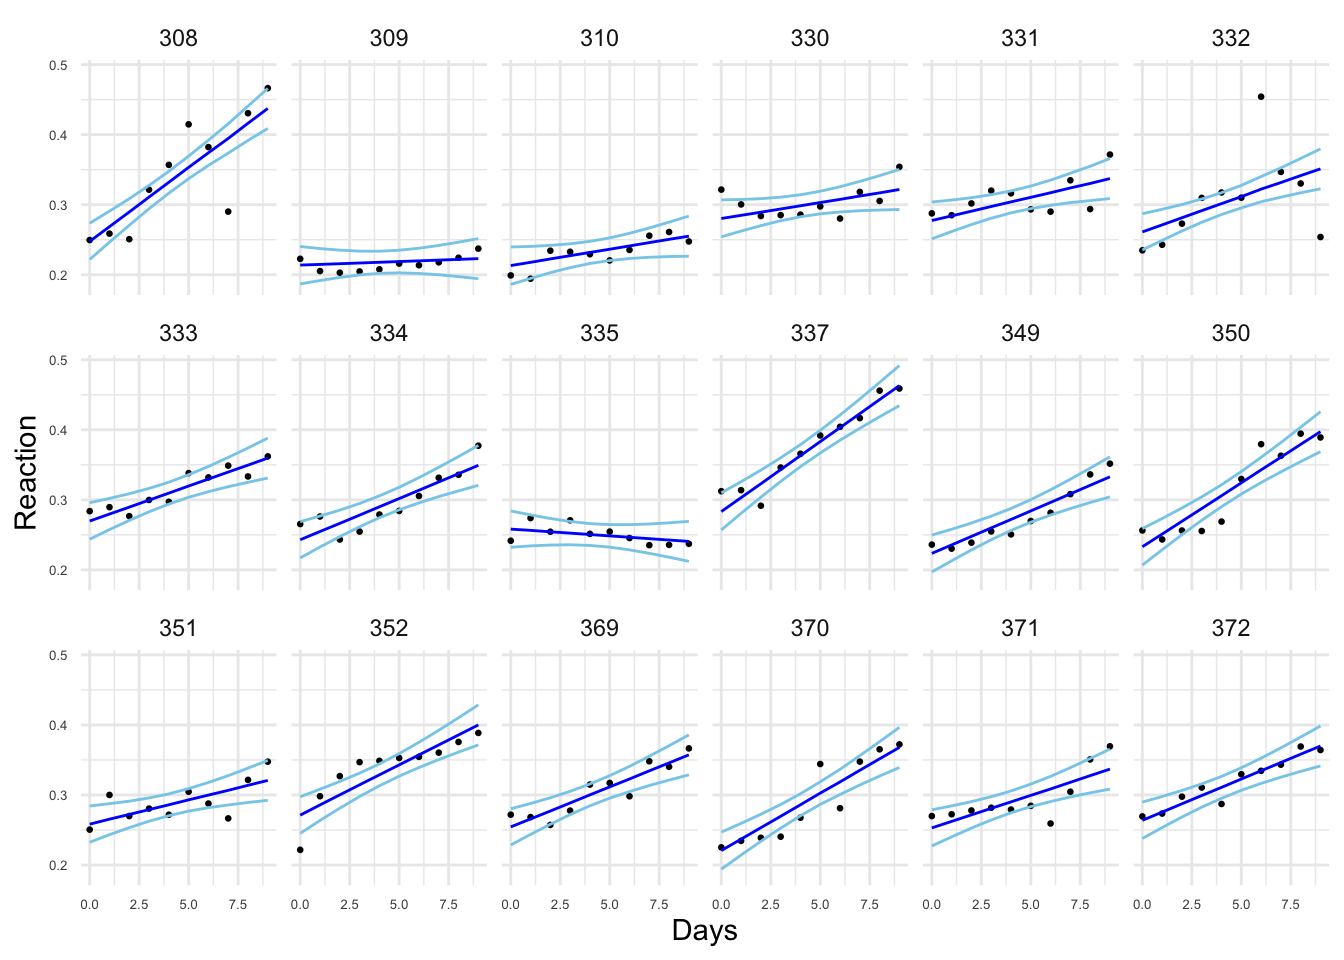
\includegraphics{02-anova_files/figure-latex/sleep2-1.pdf}
En la Figura \ref{fig:sleep3} mostramos la distribución posterior de los errores de datos y aleatorios.

\begin{Shaded}
\begin{Highlighting}[]
\NormalTok{nhyp}\OtherTok{=}\FunctionTok{length}\NormalTok{(}\FunctionTok{names}\NormalTok{(fit}\SpecialCharTok{$}\NormalTok{marginals.hyperpar))}
\NormalTok{res}\OtherTok{=}\ConstantTok{NULL}
\ControlFlowTok{for}\NormalTok{(j }\ControlFlowTok{in} \DecValTok{1}\SpecialCharTok{:}\NormalTok{nhyp)\{}
\NormalTok{    res}\OtherTok{=}\FunctionTok{rbind}\NormalTok{(res,}\FunctionTok{data.frame}\NormalTok{(}
    \FunctionTok{inla.tmarginal}\NormalTok{(}\ControlFlowTok{function}\NormalTok{(tau) tau}\SpecialCharTok{\^{}}\NormalTok{(}\SpecialCharTok{{-}}\DecValTok{1}\SpecialCharTok{/}\DecValTok{2}\NormalTok{),fit}\SpecialCharTok{$}\NormalTok{marginals.hyperpar[[j]]),}
                         \AttributeTok{id=}\FunctionTok{str\_sub}\NormalTok{(}\FunctionTok{names}\NormalTok{(fit}\SpecialCharTok{$}\NormalTok{marginals.hyperpar)[j], }\AttributeTok{start =}\DecValTok{15}\NormalTok{)))}
\NormalTok{\}}
\FunctionTok{ggplot}\NormalTok{(res,}\FunctionTok{aes}\NormalTok{(}\AttributeTok{x=}\NormalTok{x,}\AttributeTok{y=}\NormalTok{y))}\SpecialCharTok{+}
  \FunctionTok{geom\_line}\NormalTok{(}\FunctionTok{aes}\NormalTok{(}\AttributeTok{color=}\NormalTok{id))}\SpecialCharTok{+}
  \FunctionTok{labs}\NormalTok{(}\AttributeTok{x=}\FunctionTok{expression}\NormalTok{(sigma),}\AttributeTok{y=}\StringTok{""}\NormalTok{)}\SpecialCharTok{+}
  \FunctionTok{theme}\NormalTok{(}\AttributeTok{legend.position=}\StringTok{"top"}\NormalTok{,}
        \AttributeTok{legend.title=}\FunctionTok{element\_blank}\NormalTok{(),}
        \AttributeTok{legend.text =} \FunctionTok{element\_text}\NormalTok{(}\AttributeTok{size=}\DecValTok{5}\NormalTok{))}
\end{Highlighting}
\end{Shaded}

\begin{figure}
\centering
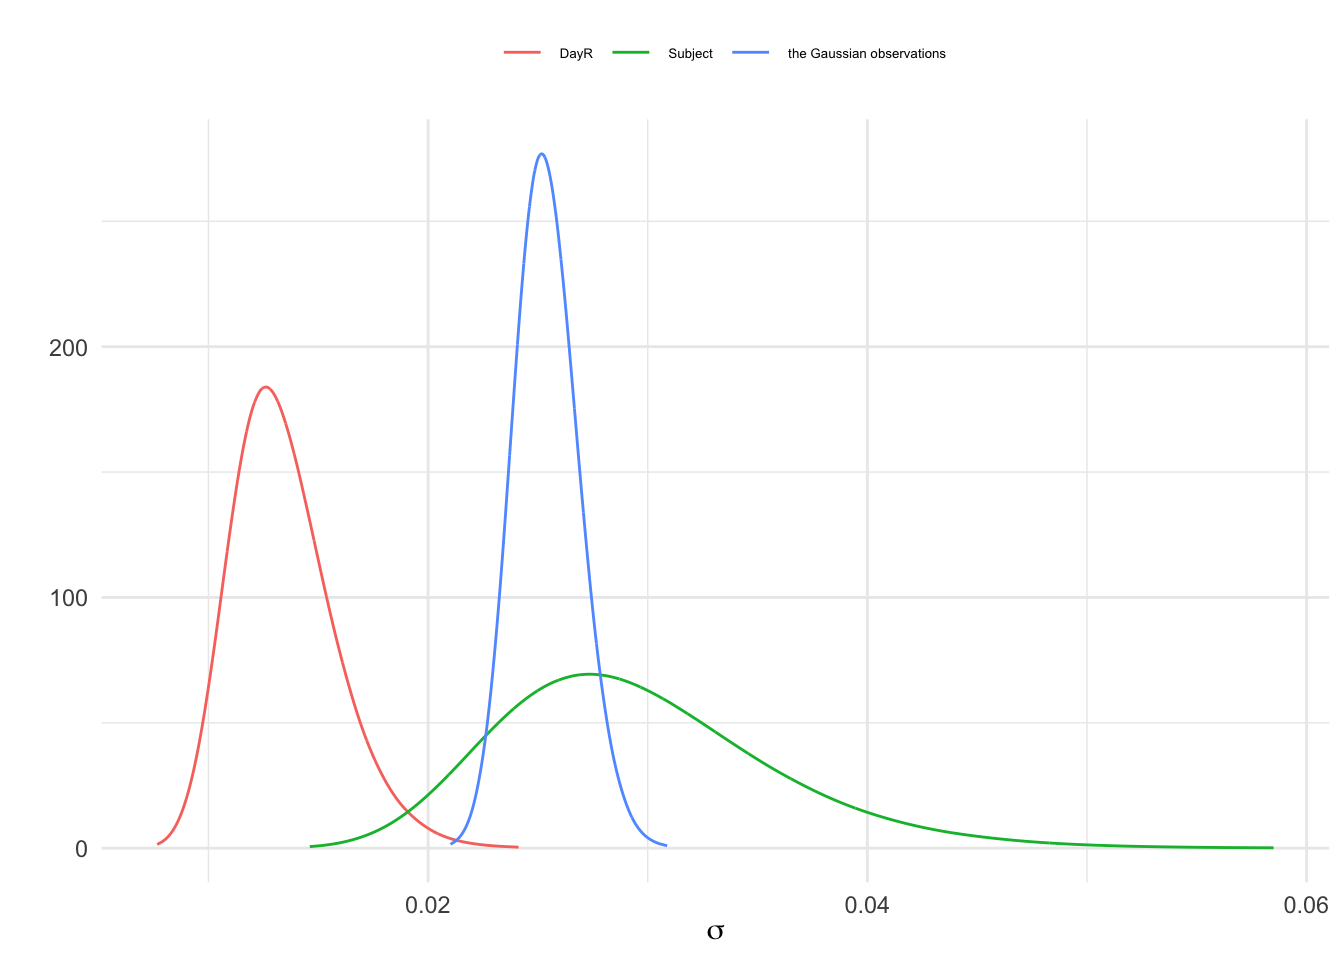
\includegraphics{02-anova_files/figure-latex/sleep3-1.pdf}
\caption{\label{fig:sleep3}Distribución posterior del error de los datos y el error aleatorio}
\end{figure}

\hypertarget{efectos-anidados}{%
\subsection{Efectos anidados}\label{efectos-anidados}}

Hablamos de efectos anidados cuando cada miembro de un grupo está contenido completamente dentro de una única unidad de otro grupo. Que un factor A esté anidado en otro B, implica que cada nivel de B contiene niveles distintos de A, esto es, cada nivel de A está vinculado solo a algún nivel de B.

La base de datos \texttt{eggs} en la librería \href{https://cran.r-project.org/web/packages/faraway/faraway.pdf}{\texttt{faraway}} nos resulta útil para describir este tipo de modelos con efectos anidados. Estos datos son los resultantes de un experimento para testar la consistencia en los tests de laboratorio que realizaban laboratorios distintos, técnicos distintos. Para ello se dividió en varias muestras un tarro de polvo de huevo seco homogeneizado (con idéntico contenido graso). Se enviaron 4 muestras a cada uno de los 6 laboratorios. De esas 4 muestras, 2 se etiquetaron como G y 2 como H (aun siendo idénticas). Se dieron instrucciones a los laboratorios de dar dos muestras a dos técnicos distintos. Los técnicos recibieron instrucciones de dividir sus muestras en dos partes y medir el contenido graso de cada una. Así, cada laboratorio reportó 8 mediciones del contenido graso (\texttt{Fat}), cada técnico 4 mediciones, con 2 réplicas en cada una de las dos muestras.

Realmente, el laboratorio, el técnico y la muestra solo deberían generar variabilidad en la respuesta, pero en ningún caso generar mediciones distintas. Estamos pues interesados en investigar la magnitud del error debido al laboratorio, al técnico y a la identificación de muestras. Es por ello que tiene sentido considerarlos efectos aleatorios.

Tenemos así en este ejemplo, a los técnicos (\texttt{Technician}) anidados en los laboratorios (\texttt{Lab}). En la Figura \ref{fig:eggs1} se muestra claramente la variación entre laboratorios, entre técnicos, y debida al efecto irreal de tener dos muestras distintas G y H (\texttt{Sample}).

\begin{Shaded}
\begin{Highlighting}[]
\FunctionTok{data}\NormalTok{(eggs,}\AttributeTok{package=}\StringTok{"faraway"}\NormalTok{)}
\FunctionTok{ggplot}\NormalTok{(eggs,}\FunctionTok{aes}\NormalTok{(}\AttributeTok{x=}\NormalTok{Lab,}\AttributeTok{y=}\NormalTok{Fat))}\SpecialCharTok{+}
  \FunctionTok{geom\_boxplot}\NormalTok{(}\FunctionTok{aes}\NormalTok{(}\AttributeTok{color=}\NormalTok{Technician))}\SpecialCharTok{+}
  \FunctionTok{facet\_wrap}\NormalTok{(}\FunctionTok{vars}\NormalTok{(Sample))}
\end{Highlighting}
\end{Shaded}

\begin{figure}
\centering
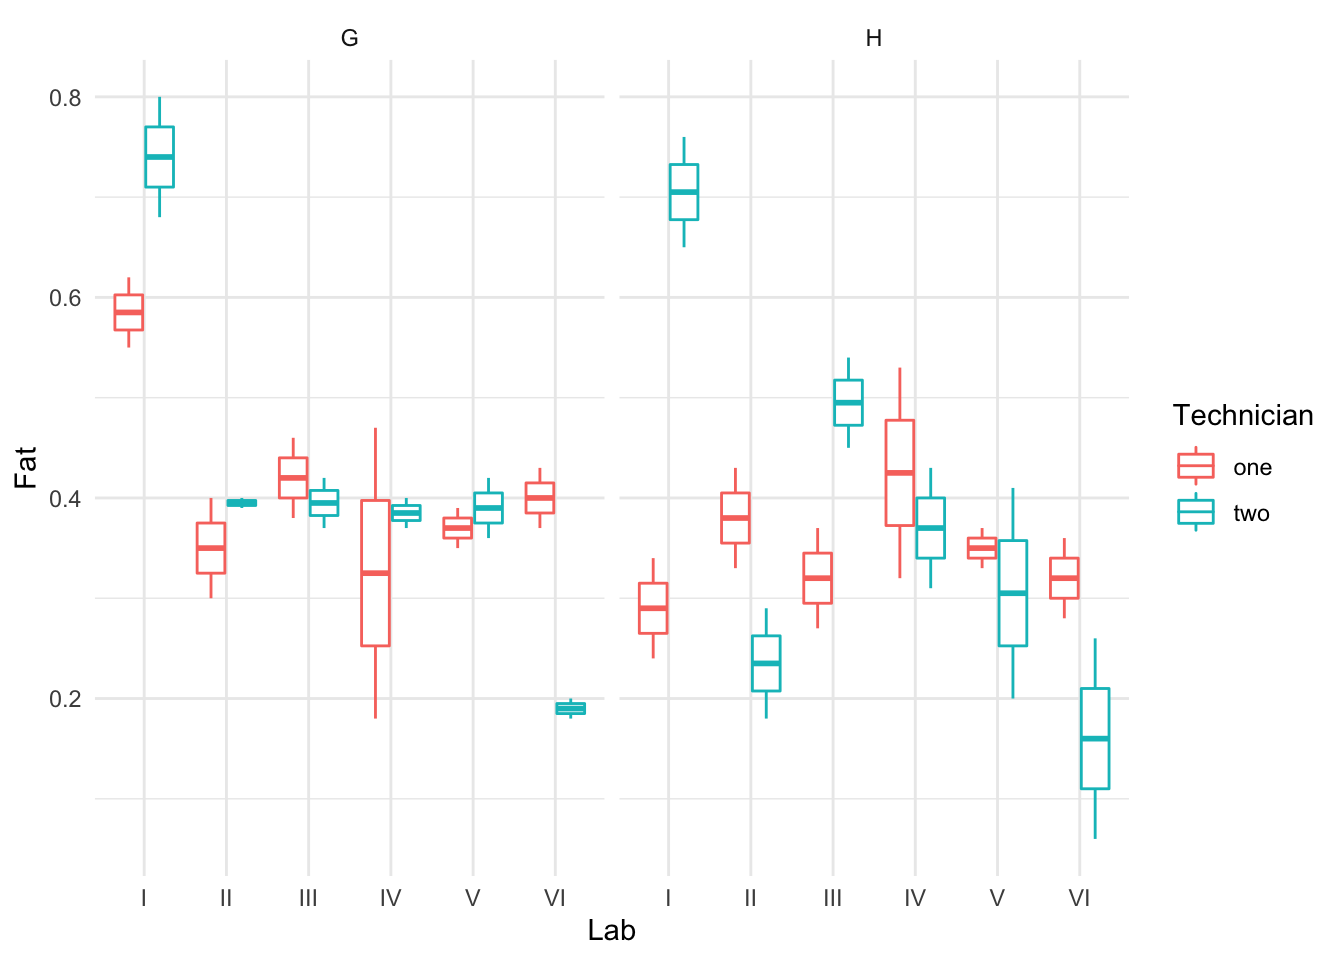
\includegraphics{02-anova_files/figure-latex/eggs1-1.pdf}
\caption{\label{fig:eggs1}Descripción de eggs: variación entre laboratorios y técnicos.}
\end{figure}

El modelo que planteamos para estimar la respuesta \(y_{ijk}\), contenido graso de la muestra \(k\) (\(k=1,2\)) del laboratorio \(i\) (\(i=1,...,6\)), por el técnico \(j\) (\(j=1,2\)) está basado como siempre, en el modelo normal, \((y_{ijk}|\mu_{ijk},\sigma^2) \sim N(\mu_{ijk},\sigma^2)\), con una media o predictor lineal representado por:

\[ \mu_{ijk}= \theta + \alpha_i^{lab} + \beta_{j:i}^{tec} + \gamma_{k:(j:i)}^{sam}\]
y asumiendo en un segundo nivel del modelo las distribuciones a priori:
\begin{eqnarray*}
\theta &\sim& N(0,1000) \\
\tau=1/\sigma^2 &\sim& Ga(0.001,0.001) \\
\alpha_i^{lab}&\sim& N(0,\sigma_{lab}^2); \  i = 1,...,4 \\
\beta_{j:i}^{tec}&\sim& N(0,\sigma_{tec}^2); \  j:i = 1,...,12 \\
\gamma_{k:(j:i)}^{sam}&\sim& N(0,\sigma_{sam}^2); \ k:(j:i)=1,...,24
\end{eqnarray*}

El tercer nivel recibiría las distribuciones a priori para los hiperparámetros \(\sigma_{lab}^2, \sigma_{tec}^2,\sigma_{sam}^2\), sobre los que interesa inferir. A priori, con mínima información asumiremos \(GaI(0.001,0.001)\).

Para especificar en INLA los efectos anidados hemos de recurrir a la matriz del modelo, \texttt{model.matrix()}, para crear las matrices de los efectos aleatorios anidados.

A continuación hemos de crear los correspondientes índices, de longitud similar a la del número de registros en la base de datos, para aplicarles las correspondientes matrices de efectos anidados, y ya proceder con el ajuste como habitualmente hacemos.

\begin{Shaded}
\begin{Highlighting}[]
\CommentTok{\# matrices de efectos aleatorios anidados}
\NormalTok{Zlt }\OtherTok{\textless{}{-}} \FunctionTok{as}\NormalTok{(}\FunctionTok{model.matrix}\NormalTok{( }\SpecialCharTok{\textasciitilde{}} \DecValTok{0} \SpecialCharTok{+}\NormalTok{ Lab}\SpecialCharTok{:}\NormalTok{Technician, }\AttributeTok{data =}\NormalTok{ eggs), }\StringTok{"Matrix"}\NormalTok{)}
\NormalTok{Zlts }\OtherTok{\textless{}{-}} \FunctionTok{as}\NormalTok{(}\FunctionTok{model.matrix}\NormalTok{( }\SpecialCharTok{\textasciitilde{}} \DecValTok{0} \SpecialCharTok{+}\NormalTok{ Lab}\SpecialCharTok{:}\NormalTok{Technician}\SpecialCharTok{:}\NormalTok{Sample, }\AttributeTok{data =}\NormalTok{ eggs), }\StringTok{"Matrix"}\NormalTok{)}

\CommentTok{\# índices para aplicar los efectos aleatorios}
\NormalTok{eggs}\SpecialCharTok{$}\NormalTok{IDt }\OtherTok{=}\NormalTok{ eggs}\SpecialCharTok{$}\NormalTok{IDts }\OtherTok{=} \DecValTok{1}\SpecialCharTok{:}\FunctionTok{nrow}\NormalTok{(eggs)}

\CommentTok{\# Ajuste}
\NormalTok{prec.prior}\OtherTok{=}\FunctionTok{list}\NormalTok{(}\AttributeTok{prec=}\FunctionTok{list}\NormalTok{(}\AttributeTok{param=}\FunctionTok{c}\NormalTok{(}\FloatTok{0.001}\NormalTok{,}\FloatTok{0.001}\NormalTok{)))}
\NormalTok{formula }\OtherTok{=}\NormalTok{ Fat }\SpecialCharTok{\textasciitilde{}} \DecValTok{1} \SpecialCharTok{+} \FunctionTok{f}\NormalTok{(Lab,}\AttributeTok{model=}\StringTok{"iid"}\NormalTok{,}\AttributeTok{hyper=}\NormalTok{prec.prior) }\SpecialCharTok{+}
  \FunctionTok{f}\NormalTok{(IDt,}\AttributeTok{model=}\StringTok{"z"}\NormalTok{,}\AttributeTok{Z=}\NormalTok{Zlt,}\AttributeTok{hyper=}\NormalTok{prec.prior)}\SpecialCharTok{+}
  \FunctionTok{f}\NormalTok{(IDts,}\AttributeTok{model=}\StringTok{"z"}\NormalTok{,}\AttributeTok{Z=}\NormalTok{Zlts,}\AttributeTok{hyper=}\NormalTok{prec.prior)}

\NormalTok{fit }\OtherTok{\textless{}{-}} \FunctionTok{inla}\NormalTok{(formula,}\AttributeTok{data =}\NormalTok{ eggs, }
            \AttributeTok{control.predictor =} \FunctionTok{list}\NormalTok{(}\AttributeTok{compute =} \ConstantTok{TRUE}\NormalTok{), }
            \AttributeTok{control.family=}\FunctionTok{list}\NormalTok{(}\AttributeTok{hyper=}\NormalTok{prec.prior),}
            \AttributeTok{control.fixed=}\FunctionTok{list}\NormalTok{(}\AttributeTok{prec.intercept=}\FloatTok{0.001}\NormalTok{))}
\CommentTok{\# inferencias de interés}
\FunctionTok{round}\NormalTok{(fit}\SpecialCharTok{$}\NormalTok{summary.hyperpar,}\DecValTok{4}\NormalTok{)}
\CommentTok{\#\textgreater{}                                             mean       sd}
\CommentTok{\#\textgreater{} Precision for the Gaussian observations 142.0221  39.6763}
\CommentTok{\#\textgreater{} Precision for Lab                       349.8905 651.0955}
\CommentTok{\#\textgreater{} Precision for IDt                       206.0418 210.4896}
\CommentTok{\#\textgreater{} Precision for IDts                      366.9427 335.2837}
\CommentTok{\#\textgreater{}                                         0.025quant 0.5quant}
\CommentTok{\#\textgreater{} Precision for the Gaussian observations    77.8353 137.4884}
\CommentTok{\#\textgreater{} Precision for Lab                          22.4901 170.1977}
\CommentTok{\#\textgreater{} Precision for IDt                          26.6549 144.1431}
\CommentTok{\#\textgreater{} Precision for IDts                         59.8945 270.7277}
\CommentTok{\#\textgreater{}                                         0.975quant mode}
\CommentTok{\#\textgreater{} Precision for the Gaussian observations   232.9086   NA}
\CommentTok{\#\textgreater{} Precision for Lab                        1808.5093   NA}
\CommentTok{\#\textgreater{} Precision for IDt                         762.1928   NA}
\CommentTok{\#\textgreater{} Precision for IDts                       1256.5620   NA}
\end{Highlighting}
\end{Shaded}

\begin{Shaded}
\begin{Highlighting}[]
\NormalTok{nhyp}\OtherTok{=}\FunctionTok{length}\NormalTok{(}\FunctionTok{names}\NormalTok{(fit}\SpecialCharTok{$}\NormalTok{marginals.hyperpar))}
\NormalTok{res}\OtherTok{=}\ConstantTok{NULL}
\ControlFlowTok{for}\NormalTok{(j }\ControlFlowTok{in} \DecValTok{1}\SpecialCharTok{:}\NormalTok{nhyp)\{}
\NormalTok{    res}\OtherTok{=}\FunctionTok{rbind}\NormalTok{(res,}\FunctionTok{data.frame}\NormalTok{(}
    \FunctionTok{inla.tmarginal}\NormalTok{(}\ControlFlowTok{function}\NormalTok{(tau) tau}\SpecialCharTok{\^{}}\NormalTok{(}\SpecialCharTok{{-}}\DecValTok{1}\SpecialCharTok{/}\DecValTok{2}\NormalTok{),fit}\SpecialCharTok{$}\NormalTok{marginals.hyperpar[[j]]),}
                         \AttributeTok{id=}\FunctionTok{str\_sub}\NormalTok{(}\FunctionTok{names}\NormalTok{(fit}\SpecialCharTok{$}\NormalTok{marginals.hyperpar)[j], }\AttributeTok{start =}\DecValTok{15}\NormalTok{)))}
\NormalTok{\}}
\FunctionTok{ggplot}\NormalTok{(res,}\FunctionTok{aes}\NormalTok{(}\AttributeTok{x=}\NormalTok{x,}\AttributeTok{y=}\NormalTok{y))}\SpecialCharTok{+}
  \FunctionTok{geom\_line}\NormalTok{(}\FunctionTok{aes}\NormalTok{(}\AttributeTok{color=}\NormalTok{id))}\SpecialCharTok{+}
  \FunctionTok{labs}\NormalTok{(}\AttributeTok{x=}\FunctionTok{expression}\NormalTok{(sigma),}\AttributeTok{y=}\StringTok{""}\NormalTok{)}\SpecialCharTok{+}
  \FunctionTok{theme}\NormalTok{(}\AttributeTok{legend.position=}\StringTok{"top"}\NormalTok{,}
        \AttributeTok{legend.title=}\FunctionTok{element\_blank}\NormalTok{(),}
        \AttributeTok{legend.text =} \FunctionTok{element\_text}\NormalTok{(}\AttributeTok{size=}\DecValTok{5}\NormalTok{))}
\end{Highlighting}
\end{Shaded}

\begin{figure}
\centering
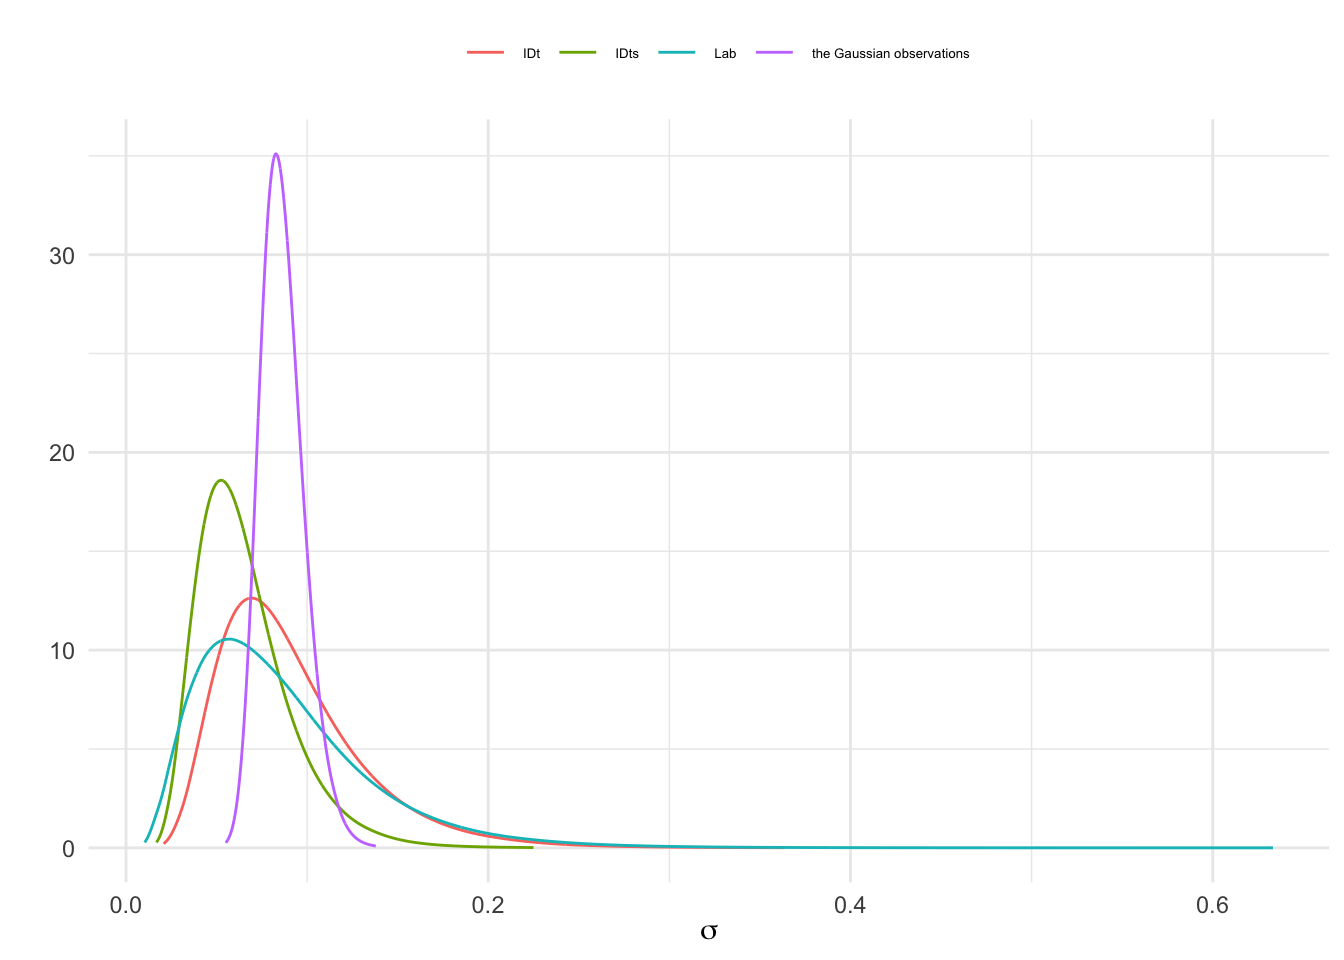
\includegraphics{02-anova_files/figure-latex/eggs2-1.pdf}
\caption{\label{fig:eggs2}Distribución posterior del error de los datos y el error aleatorio}
\end{figure}

Alternativamente podríamos crear una variable índice a partir de las matrices de efectos aleatorios, para utilizarlas con \texttt{model="iid"} para describir los efectos aleatorios:

\begin{Shaded}
\begin{Highlighting}[]
\NormalTok{eggs}\SpecialCharTok{$}\NormalTok{labtech }\OtherTok{\textless{}{-}} \FunctionTok{as.factor}\NormalTok{(}\FunctionTok{apply}\NormalTok{(Zlt, }\DecValTok{1}\NormalTok{, }\ControlFlowTok{function}\NormalTok{(x)\{}\FunctionTok{names}\NormalTok{(x)[x }\SpecialCharTok{==} \DecValTok{1}\NormalTok{]\}))}
\NormalTok{eggs}\SpecialCharTok{$}\NormalTok{labtechsamp }\OtherTok{\textless{}{-}} \FunctionTok{as.factor}\NormalTok{(}\FunctionTok{apply}\NormalTok{(Zlts, }\DecValTok{1}\NormalTok{, }\ControlFlowTok{function}\NormalTok{(x)\{}\FunctionTok{names}\NormalTok{(x)[x }\SpecialCharTok{==} \DecValTok{1}\NormalTok{]\}))}

\NormalTok{formula}\OtherTok{=}\NormalTok{Fat }\SpecialCharTok{\textasciitilde{}} \DecValTok{1} \SpecialCharTok{+} \FunctionTok{f}\NormalTok{(Lab, }\AttributeTok{model =} \StringTok{"iid"}\NormalTok{, }\AttributeTok{hyper =}\NormalTok{ prec.prior) }\SpecialCharTok{+}
    \FunctionTok{f}\NormalTok{(labtech, }\AttributeTok{model =} \StringTok{"iid"}\NormalTok{, }\AttributeTok{hyper =}\NormalTok{ prec.prior) }\SpecialCharTok{+}
  \FunctionTok{f}\NormalTok{(labtechsamp, }\AttributeTok{model =} \StringTok{"iid"}\NormalTok{, }\AttributeTok{hyper =}\NormalTok{ prec.prior)}
\NormalTok{fit}\OtherTok{=}\FunctionTok{inla}\NormalTok{(formula, }\AttributeTok{data =}\NormalTok{ eggs, }
            \AttributeTok{control.predictor =} \FunctionTok{list}\NormalTok{(}\AttributeTok{compute =} \ConstantTok{TRUE}\NormalTok{), }
            \AttributeTok{control.family=}\FunctionTok{list}\NormalTok{(}\AttributeTok{hyper=}\NormalTok{prec.prior),}
         \AttributeTok{control.fixed=}\FunctionTok{list}\NormalTok{(}\AttributeTok{prec.intercept=}\FloatTok{0.001}\NormalTok{))}
\FunctionTok{round}\NormalTok{(fit}\SpecialCharTok{$}\NormalTok{summary.fixed,}\DecValTok{4}\NormalTok{)}
\CommentTok{\#\textgreater{}               mean     sd 0.025quant 0.5quant 0.975quant}
\CommentTok{\#\textgreater{} (Intercept) 0.3875 0.0554     0.2756   0.3875     0.4994}
\CommentTok{\#\textgreater{}             mode kld}
\CommentTok{\#\textgreater{} (Intercept)   NA   0}
\FunctionTok{round}\NormalTok{(fit}\SpecialCharTok{$}\NormalTok{summary.hyperpar,}\DecValTok{4}\NormalTok{)}
\CommentTok{\#\textgreater{}                                             mean       sd}
\CommentTok{\#\textgreater{} Precision for the Gaussian observations 141.9183  39.6197}
\CommentTok{\#\textgreater{} Precision for Lab                       349.8687 651.1198}
\CommentTok{\#\textgreater{} Precision for labtech                   206.0426 210.4997}
\CommentTok{\#\textgreater{} Precision for labtechsamp               366.9591 335.2916}
\CommentTok{\#\textgreater{}                                         0.025quant 0.5quant}
\CommentTok{\#\textgreater{} Precision for the Gaussian observations    77.8083 137.3958}
\CommentTok{\#\textgreater{} Precision for Lab                          22.4884 170.1766}
\CommentTok{\#\textgreater{} Precision for labtech                      26.6547 144.1403}
\CommentTok{\#\textgreater{} Precision for labtechsamp                  59.8978 270.7425}
\CommentTok{\#\textgreater{}                                         0.975quant mode}
\CommentTok{\#\textgreater{} Precision for the Gaussian observations   232.6622   NA}
\CommentTok{\#\textgreater{} Precision for Lab                        1808.4661   NA}
\CommentTok{\#\textgreater{} Precision for labtech                     762.2166   NA}
\CommentTok{\#\textgreater{} Precision for labtechsamp                1256.5985   NA}
\end{Highlighting}
\end{Shaded}

En la Figura \ref{fig:eggs3} se muestra la distribución posterior del error de los datos y de los errores aleatorios.

\begin{Shaded}
\begin{Highlighting}[]
\NormalTok{nhyp}\OtherTok{=}\FunctionTok{length}\NormalTok{(}\FunctionTok{names}\NormalTok{(fit}\SpecialCharTok{$}\NormalTok{marginals.hyperpar))}
\NormalTok{res}\OtherTok{=}\ConstantTok{NULL}
\ControlFlowTok{for}\NormalTok{(j }\ControlFlowTok{in} \DecValTok{1}\SpecialCharTok{:}\NormalTok{nhyp)\{}
\NormalTok{    res}\OtherTok{=}\FunctionTok{rbind}\NormalTok{(res,}\FunctionTok{data.frame}\NormalTok{(}
    \FunctionTok{inla.tmarginal}\NormalTok{(}\ControlFlowTok{function}\NormalTok{(tau) tau}\SpecialCharTok{\^{}}\NormalTok{(}\SpecialCharTok{{-}}\DecValTok{1}\SpecialCharTok{/}\DecValTok{2}\NormalTok{),fit}\SpecialCharTok{$}\NormalTok{marginals.hyperpar[[j]]),}
                         \AttributeTok{id=}\FunctionTok{str\_sub}\NormalTok{(}\FunctionTok{names}\NormalTok{(fit}\SpecialCharTok{$}\NormalTok{marginals.hyperpar)[j], }\AttributeTok{start =}\DecValTok{15}\NormalTok{)))}
\NormalTok{\}}
\FunctionTok{ggplot}\NormalTok{(res,}\FunctionTok{aes}\NormalTok{(}\AttributeTok{x=}\NormalTok{x,}\AttributeTok{y=}\NormalTok{y))}\SpecialCharTok{+}
  \FunctionTok{geom\_line}\NormalTok{(}\FunctionTok{aes}\NormalTok{(}\AttributeTok{color=}\NormalTok{id))}\SpecialCharTok{+}
  \FunctionTok{labs}\NormalTok{(}\AttributeTok{x=}\FunctionTok{expression}\NormalTok{(sigma),}\AttributeTok{y=}\StringTok{""}\NormalTok{)}\SpecialCharTok{+}
  \FunctionTok{theme}\NormalTok{(}\AttributeTok{legend.position=}\StringTok{"top"}\NormalTok{,}
        \AttributeTok{legend.title=}\FunctionTok{element\_blank}\NormalTok{(),}
        \AttributeTok{legend.text =} \FunctionTok{element\_text}\NormalTok{(}\AttributeTok{size=}\DecValTok{5}\NormalTok{))}
\end{Highlighting}
\end{Shaded}

\begin{figure}
\centering
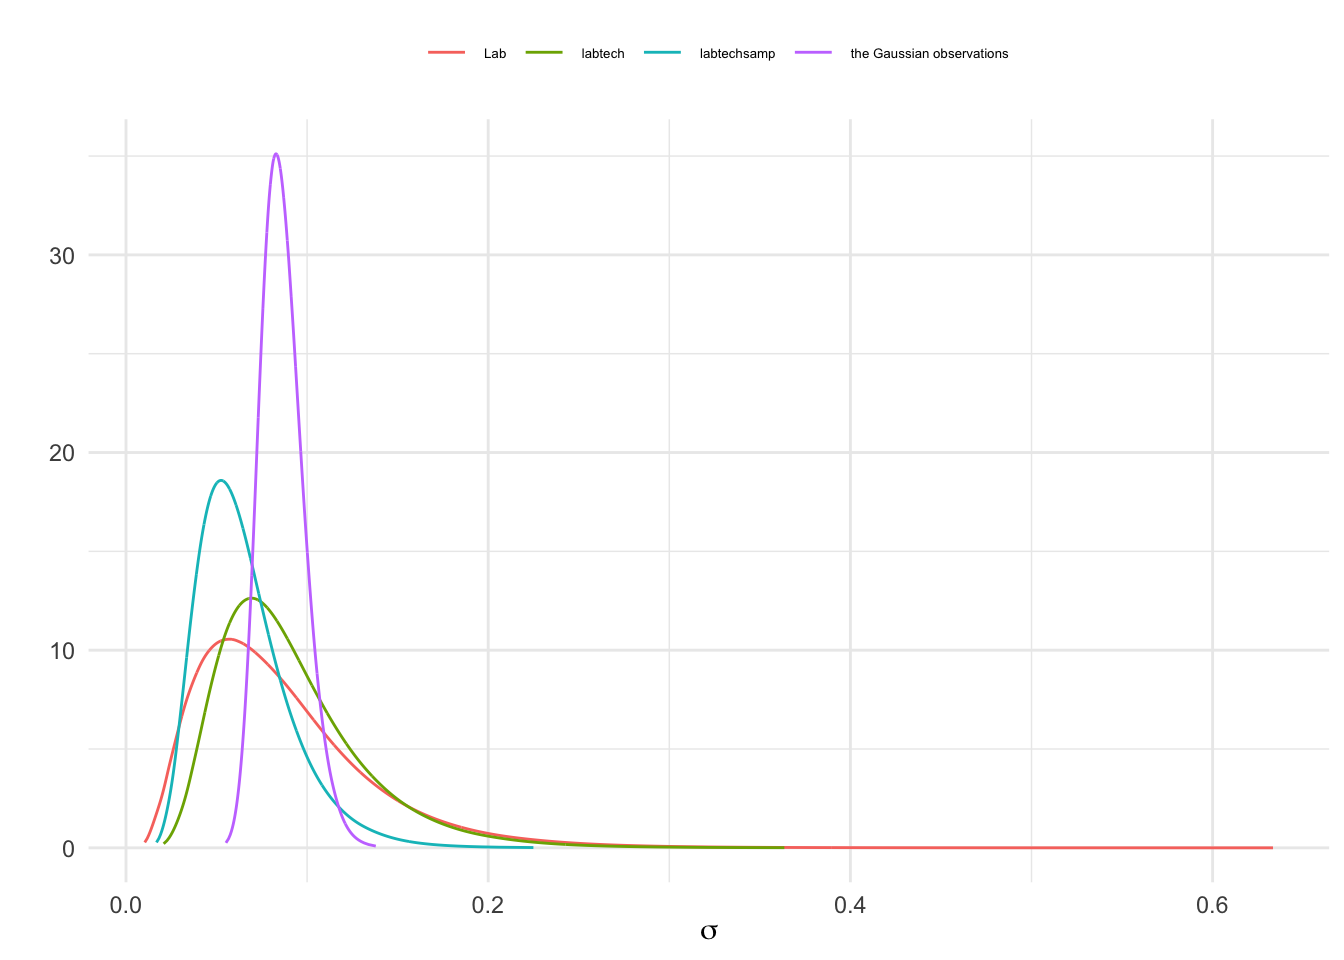
\includegraphics{02-anova_files/figure-latex/eggs3-1.pdf}
\caption{\label{fig:eggs3}Distribución posterior del error de los datos y el error aleatorio}
\end{figure}

\hypertarget{conclusiones-1}{%
\section{Conclusiones}\label{conclusiones-1}}

Hasta aquí desarrollamos los modelos lineales basados en Anova, esto es, en la integración de factores de clasificación como variables que van a explicar diferencias en la respuesta, como los efectos fijos, o variabilidad extra en los datos, como los efectos aleatorios, a veces incluso con otros predictores de tipo numérico, e incluso interaccionando con ellos.

\hypertarget{glm}{%
\chapter{Modelos lineales generalizados}\label{glm}}

Los modelos lineales generalizados (Generalized Linear Models or GLM), son una clase de modelos introducidos por Nelder y Wedderburn (1972) y McCullagh y Nelder (1989), con el objetivo de extender la regresión lineal al caso en el que la variable dependiente no se distribuya necesariamente según una normal, pero su distribución todavía pertenezca a la familia exponencial (Binomial, Poisson, Gamma, Gausiana inversa básicamente). Trabajamos a continuación con dos de los GLM más comunes en epidemiología y ciencias sociales: la regresión logística y la de Poisson, mostrando cómo usar R-INLA.

Un modelo lineal generalizado está basado en asumir, además de una distribución de los datos dentro de la familia exponencial, una relación lineal entre cierta transformación del valor esperado de la respuesta \(E(y_i)\) y los predictores disponibles, sean covariables, efectos fijos, efectos aleatorios, o incluso alguna función de estos.

Si \(y\) representa una respuesta observada, \(x_1,x_2,..\) una serie de covariables o efectos fijos, y \(z_1,z_2,...\) efectos aleatorios, el valor esperado de la respuesta lo denotamos como \(\mu\), que

\[E(y_i|x,z,\theta)=\mu_i\]
Pues bien, la relación entre esta media \(\mu\) y un predictor lineal \(\eta\) que construimos a partir de los predictores disponibles, viene dado por una función link \(g\) tal que:

\[g(\mu_i)=\eta_i=\mu + \beta_1 x_{1i} +   \beta_2 x_{2i} +...+ z_{1i} + z_{2i}+...\]

Todos los parámetros involucrados en el predictor lineal \(\eta\) son los efectos latentes del modelo (fijos o aleatorios). Estos, junto con el resto de parámetros definidos en este primer nivel de la modelización (nivel de datos), han de modelizarse a continuación, en un segundo nivel del modelo, con sus correspondientes distribuciones a priori.

El predictor lineal \(\eta\) está relacionado linealmente con los predictores según:
\[\eta_i=\mu + \beta_1 x_{1i} +   \beta_2 x_{2i} +...+ z_{1i} + z_{2i}+...\]
relación que se suele representar en forma matricial como
\[\eta=X\beta + Z u\]

Los modelos lineales que hemos visto antes (regresión, anova, ancova, modelos mixtos) se engloban dentro del modelo lineal generalizado.

El argumento \texttt{control.predictor=list(compute=TRUE)} en la función \texttt{inla} permite obtener las distribuciones predictivas para el predictor lineal, que en estos casos es distinto a los valores ajustados, \texttt{fit\$summary.fitted}. Además para obtener la distribución marginal de los valores ajustados y predichos necesitamos incorporar a la función \texttt{inla} el argumento \texttt{control.compute=list(return.marginals.predictor=TRUE)}, y ya con todo ello podemos:

\begin{itemize}
\tightlist
\item
  \texttt{fit\$summary.linear.predictor} resumir la inferencia posterior sobre los
  predictores lineales (distintos a los fitted cuando hay una función \emph{link})
\item
  \texttt{fit\$marginals.linear.predictor} graficar y describir las distribuciones posteriores marginales para los predictores lineales
\end{itemize}

\hypertarget{modelos-jeruxe1rquicos-bayesianos}{%
\section{Modelos jerárquicos bayesianos}\label{modelos-jeruxe1rquicos-bayesianos}}

A lo largo del curso ya hemos ido comentando en ocasiones, algo sobre la especificación de un modelo en varios niveles. Presentamos ya de lleno estos modelos lineales generalizados como modelos multi-nivel o modelos jerárquicos, denominados así porque se va especificando por niveles (o jerarquías) la información disponible sobre todo aquello que es desconocido, distribución de los datos y parámetros.

Un modelo bayesiano se modeliza a través de un modelo jerárquico o multinivel en el que en el nivel I se define la distribución asumida sobre la variable respuesta y que determina la verosimilitud. Esta variable depende de unos parámetros que definen los efectos fijos y aleatorios, y para los que hay que proporcionar la información previa disponible a través de una distribución a priori en el segundo nivel del modelo jerárquico. La distribución a priori para los efectos fijos generalmente será común a todos ellos, mientras que la distribución a priori para los efectos aleatorios estará vinculada a otros hiperparámetros para los que también será preciso especificar una distribución a priori en un tercer nivel de la modelización, y así sucesivamente.

\begin{eqnarray*}
Nivel I &&\\
( y | X, Z, \theta) &\sim & f(y|x,z,\theta) \text{f en fam.exponencial}\\
&& E(y|x,z,\theta)=\mu; Var(y|x,z,\theta)=\Sigma \\
&& g(\mu)=\eta=X\beta + Z u \\
Nivel II &&\\
\beta &\sim & N(0,\sigma_{\beta}), \text{ con un valor dado  para } \sigma_{\beta} \\
u|\sigma_u^2 &\sim_{iid}&  N(0,{\sigma_u^2}) \\
\Sigma|s &\sim& F_{\Sigma|s} \\
Nivel III &&\\
\sigma_u^2 &\sim&  F_{\sigma} \\
s &\sim&  F_{s}
\end{eqnarray*}

\hypertarget{regresiuxf3n-loguxedstica}{%
\section{Regresión logística}\label{regresiuxf3n-loguxedstica}}

La regresión logística es el modelo estándar para respuestas binarias (éxitos/fracasos). Tiene dos variaciones, en función de si la respuesta representa observaciones individuales (0/1) o conteos (de éxitos) en grupos de sujetos.

Si las observaciones son individualizadas, entonces

\[y_i|\pi_i \sim Ber(\pi_i), \ i=1,...,n\]
En el caso de que sean conteos en grupos,

\[y_i|\pi_i\sim Bin(n_i,\pi_i), \ i=1,...,n\]
siendo \(n_i\) el tamaño de cada uno de los \(n\) grupos disponibles, y \(\pi_i\) la probabilidad de éxito (output de interés).

La relación entre el predictor lineal \(\eta\) construido con los predictores disponibles \(x=(x_{1},...x_{M})\) y la probabilidad \(\pi\) se especifica a través de la función \emph{logit}:
\[logit(\pi)=log\left(\frac{\pi}{1-\pi}\right)=\eta=X\beta=\beta_0+\sum_{j=1}^M \beta_j x_{j}\]
de forma que
\[\pi=logit^{-1}(X\beta)=\frac{exp(X\beta)}{1-exp(X\beta)}\]
Una vez especificado el modelo, si no hay información previa disponible sobre los efectos (fijos) \({\beta_o,\beta_1,...\beta_M}\), se asumen distribuciones a priori independientes y normales con media cero y varianza muy grande.

\hypertarget{interpretaciuxf3n-de-los-coeficientes-en-la-regresiuxf3n-logit}{%
\subsection*{Interpretación de los coeficientes en la regresión logit}\label{interpretaciuxf3n-de-los-coeficientes-en-la-regresiuxf3n-logit}}
\addcontentsline{toc}{subsection}{Interpretación de los coeficientes en la regresión logit}

Puesto que \(X\beta=\beta_0+\sum_{j=1}^M \beta_j x_{j}\), la interceptación del predictor lineal \(\beta_0\) se interpreta como los predictores toman el valor cero si son numéricos, o están en el nivel de referencia (para la estimación) si son categóricos, \(\eta(X=0)=\beta_0=logit(\pi)\). En consecuencia, el logit inverso de \(\beta_0\) se interpreta como la probabilidad de éxito \(\pi_i\) cuando los predictores están en su nivel de referencia o son cero.
\[logit^{-1}(\beta_0)=Pr(y=1|X=0).\]

En cuanto a la interpretación de cualquier otro coeficiente de regresión en el predictor lineal, como \(\beta_1\), echamos mano del concepto de \emph{odds} y \emph{odds ratio}.

Los odds ratio, OR, comparan, a través de un cociente, las posibilidades a favor de un evento \(E\) bajo condiciones A y de las posibilidades del mismo evento bajo condiciones B. Nos sirve para evaluar cuánto afecta a dicho evento el hecho de variar las condiciones de B a A.
\[OR(A,B)=\frac{Pr(E|A)/(1-Pr(E|A))}{Pr(E|B)/(1-Pr(E|B))}.\]

En el modelo logístico, nos interesa saber el efecto que tiene sobre la respuesta (realmente sobre las probabilidad de éxito) el incremento de una unidad en la variable \(x\), y para ello consideramos los odds bajo \(x\) y los odds bajo \(x+1\), y en particular el logaritmo de los odds, log-odds:
\[log.odds(x+1)=log \left( \frac{P(y=1|x+1)}{P(y=0|x+1)} \right)=log \left(\frac{\pi}{1-\pi} | x+1\right)=\beta_0+\beta_1 (x+1)\]
\[log.odds(x)=log \left(\frac{P(y=1|x)}{P(y=0|x)} \right)=log \left(\frac{\pi}{1-\pi} | x\right)=\beta_0+\beta_1 x\]
de modo que
\[log(OR(x+1,x))=log \left(\frac{ods (x+1)}{ods(x)} \right) = log.odds(x+1)-log.ods(x)= \beta_1\]
y tenemos entonces que la exponencial del coeficiente \(\beta_1\) nos da el odds ratio asociado a dicha covariable.
\[exp(\beta_1)=\frac{odds(x+1)}{odds(x)}=OR(x+1,x).\]
Es decir, el coeficiente \(\beta_1\) representa el cambio en los odds a favor de un éxito cuando se incrementa en una unidad el predictor \(x\) al que acompaña en el predictor linea. Esta interpretación es muy común en Epidemiología.

\hypertarget{intenciuxf3n-de-voto-feb2022}{%
\subsection{Intención de voto feb2022}\label{intenciuxf3n-de-voto-feb2022}}

Tenemos acceso a los datos completos obtenidos en la encuesta encargada por El País y la Cadena Ser a la empresa ``40dB'', en febrero de 2022, sobre la intención de voto nacional (\href{https://elpais.com/espana/2022-02-07/consulte-todos-los-datos-internos-de-la-encuesta-de-el-pais-cuestionarios-cruces-y-respuestas-individuales.html}{fuente}).

Queremos predecir la probabilidad de votar al partido que gobierna mayoritariamente en la actualidad, PSOE, registrado en la variable \texttt{psoe}. Vamos a utilizar como predictores dos factores que nos dicen si el sujeto tiene simpatía por ese partido, \texttt{psoe\_sim}, y si votó PSOE en las últimas elecciones \texttt{psoe\_past}; también utilizaremos la comunidad autónoma \texttt{ccaa} como un efecto aleatorio, para contabilizar posible variación extra.

\begin{Shaded}
\begin{Highlighting}[]
\NormalTok{url}\OtherTok{=}\StringTok{"https://raw.githubusercontent.com/BayesModel/data/main/barometro\_feb22.csv"}
\NormalTok{barometro\_feb22}\OtherTok{=}\FunctionTok{read.csv}\NormalTok{(url)}
\FunctionTok{names}\NormalTok{(barometro\_feb22)}
\CommentTok{\#\textgreater{}  [1] "X"                   "id"                 }
\CommentTok{\#\textgreater{}  [3] "sexo"                "edad"               }
\CommentTok{\#\textgreater{}  [5] "edad\_r"              "hab"                }
\CommentTok{\#\textgreater{}  [7] "prov"                "ccaa"               }
\CommentTok{\#\textgreater{}  [9] "edu"                 "cs"                 }
\CommentTok{\#\textgreater{} [11] "p1"                  "p2"                 }
\CommentTok{\#\textgreater{} [13] "p3"                  "p4\_1"               }
\CommentTok{\#\textgreater{} [15] "p4\_2"                "p4\_3"               }
\CommentTok{\#\textgreater{} [17] "p4\_4"                "p5"                 }
\CommentTok{\#\textgreater{} [19] "p6"                  "p7"                 }
\CommentTok{\#\textgreater{} [21] "hab\_r"               "clase\_social\_r"     }
\CommentTok{\#\textgreater{} [23] "situacion\_laboral\_r" "educacion\_r"        }
\CommentTok{\#\textgreater{} [25] "ponde"}
\NormalTok{datos}\OtherTok{=}\NormalTok{barometro\_feb22 }\SpecialCharTok{\%\textgreater{}\%}
  \FunctionTok{select}\NormalTok{(id,p2,p3,p5,ccaa) }\SpecialCharTok{\%\textgreater{}\%}
  \FunctionTok{mutate}\NormalTok{(}\AttributeTok{psoe=}\DecValTok{1}\SpecialCharTok{*}\NormalTok{(p2}\SpecialCharTok{==}\StringTok{"PSOE (Partido Socialista Obrero Español)"}\NormalTok{),}
         \AttributeTok{psoe\_simp=}\DecValTok{1}\SpecialCharTok{*}\NormalTok{(p3}\SpecialCharTok{==}\StringTok{"PSOE (Partido Socialista Obrero Español)"}\NormalTok{),}
         \AttributeTok{psoe\_past=}\DecValTok{1}\SpecialCharTok{*}\NormalTok{(p5}\SpecialCharTok{==}\StringTok{"PSOE (Partido Socialista Obrero Español)"}\NormalTok{)) }
\CommentTok{\#summary(datos)}
\end{Highlighting}
\end{Shaded}

Para ajustar el modelo utilizamos el argumento \texttt{family=binomial} y la opción \texttt{control.predictor\ =\ list(link\ =\ 1)} para establecer la función link apropiada para tener los valores ajustados en la escala correcta.

\begin{Shaded}
\begin{Highlighting}[]
\NormalTok{prec.prior}\OtherTok{=}\FunctionTok{list}\NormalTok{(}\AttributeTok{prec=}\FunctionTok{list}\NormalTok{(}\AttributeTok{param=}\FunctionTok{c}\NormalTok{(}\FloatTok{0.001}\NormalTok{,}\FloatTok{0.001}\NormalTok{)))}
\NormalTok{formula }\OtherTok{=}\NormalTok{ psoe }\SpecialCharTok{\textasciitilde{}}\NormalTok{ psoe\_simp }\SpecialCharTok{+}\NormalTok{ psoe\_past}\SpecialCharTok{+} \FunctionTok{f}\NormalTok{(ccaa,}\AttributeTok{model=}\StringTok{"iid"}\NormalTok{,}\AttributeTok{hyper=}\NormalTok{prec.prior)}
\NormalTok{fit}\OtherTok{=}\FunctionTok{inla}\NormalTok{(formula,}\AttributeTok{family=}\StringTok{"binomial"}\NormalTok{,}\AttributeTok{data=}\NormalTok{datos,}\AttributeTok{control.predictor =} \FunctionTok{list}\NormalTok{(}\AttributeTok{link =} \DecValTok{1}\NormalTok{))}
\NormalTok{fit}\SpecialCharTok{$}\NormalTok{summary.fixed}
\CommentTok{\#\textgreater{}                  mean        sd 0.025quant  0.5quant}
\CommentTok{\#\textgreater{} (Intercept) {-}3.590549 0.1897354  {-}3.998915 {-}3.578265}
\CommentTok{\#\textgreater{} psoe\_simp    3.085795 0.1865848   2.723898  3.084361}
\CommentTok{\#\textgreater{} psoe\_past    2.352348 0.1856950   1.989698  2.351803}
\CommentTok{\#\textgreater{}             0.975quant mode          kld}
\CommentTok{\#\textgreater{} (Intercept)  {-}3.251318   NA 5.820554e{-}07}
\CommentTok{\#\textgreater{} psoe\_simp     3.455832   NA 3.431097e{-}07}
\CommentTok{\#\textgreater{} psoe\_past     2.718088   NA 9.428328e{-}07}
\NormalTok{fit}\SpecialCharTok{$}\NormalTok{summary.hyperpar}
\CommentTok{\#\textgreater{}                        mean       sd 0.025quant 0.5quant}
\CommentTok{\#\textgreater{} Precision for ccaa 70.82681 251.2122   1.979164 10.70692}
\CommentTok{\#\textgreater{}                    0.975quant mode}
\CommentTok{\#\textgreater{} Precision for ccaa   588.1799   NA}
\end{Highlighting}
\end{Shaded}

Las distribuciones posteriores de los exponenciales de los efectos aleatorios se muestran en la Figura \ref{fig:eleccion2}, identificadas en verde las de efectos positivos en la media posterior del predictor lineal (log-odds \(>1\)), y en rojo las de efectos negativos, e interpretables como más y menos favorables a votar por el PSOE.

\begin{Shaded}
\begin{Highlighting}[]
\NormalTok{random }\OtherTok{=} \FunctionTok{as.data.frame}\NormalTok{(fit}\SpecialCharTok{$}\NormalTok{summary.random)}
\NormalTok{random}\SpecialCharTok{$}\NormalTok{pro}\OtherTok{=}\DecValTok{1}\SpecialCharTok{*}\FunctionTok{exp}\NormalTok{(random}\SpecialCharTok{$}\NormalTok{ccaa.mean)}\SpecialCharTok{\textgreater{}}\DecValTok{1}
\FunctionTok{ggplot}\NormalTok{(random,}\FunctionTok{aes}\NormalTok{(}\AttributeTok{x=}\FunctionTok{exp}\NormalTok{(ccaa.mean),}\AttributeTok{y=}\NormalTok{ccaa.ID)) }\SpecialCharTok{+}
  \FunctionTok{geom\_point}\NormalTok{(}\FunctionTok{aes}\NormalTok{(}\AttributeTok{color=}\NormalTok{pro))}\SpecialCharTok{+}
  \FunctionTok{geom\_errorbarh}\NormalTok{(}\FunctionTok{aes}\NormalTok{(}\AttributeTok{xmin=}\FunctionTok{exp}\NormalTok{(ccaa.}\FloatTok{0.025}\NormalTok{quant),}\AttributeTok{xmax=}\FunctionTok{exp}\NormalTok{(ccaa.}\FloatTok{0.975}\NormalTok{quant),}\AttributeTok{color=}\NormalTok{pro))}\SpecialCharTok{+}
  \FunctionTok{geom\_vline}\NormalTok{(}\AttributeTok{xintercept=}\DecValTok{1}\NormalTok{,}\AttributeTok{linetype=}\StringTok{"dotted"}\NormalTok{)}\SpecialCharTok{+}
  \FunctionTok{labs}\NormalTok{(}\AttributeTok{x=}\StringTok{"Medias y RC posteriores para el log{-}odds"}\NormalTok{,}\AttributeTok{y=}\StringTok{"Comunidad autónoma"}\NormalTok{)}\SpecialCharTok{+}
  \FunctionTok{theme}\NormalTok{(}\AttributeTok{legend.position=}\StringTok{"none"}\NormalTok{)}
\end{Highlighting}
\end{Shaded}

\begin{figure}
\centering
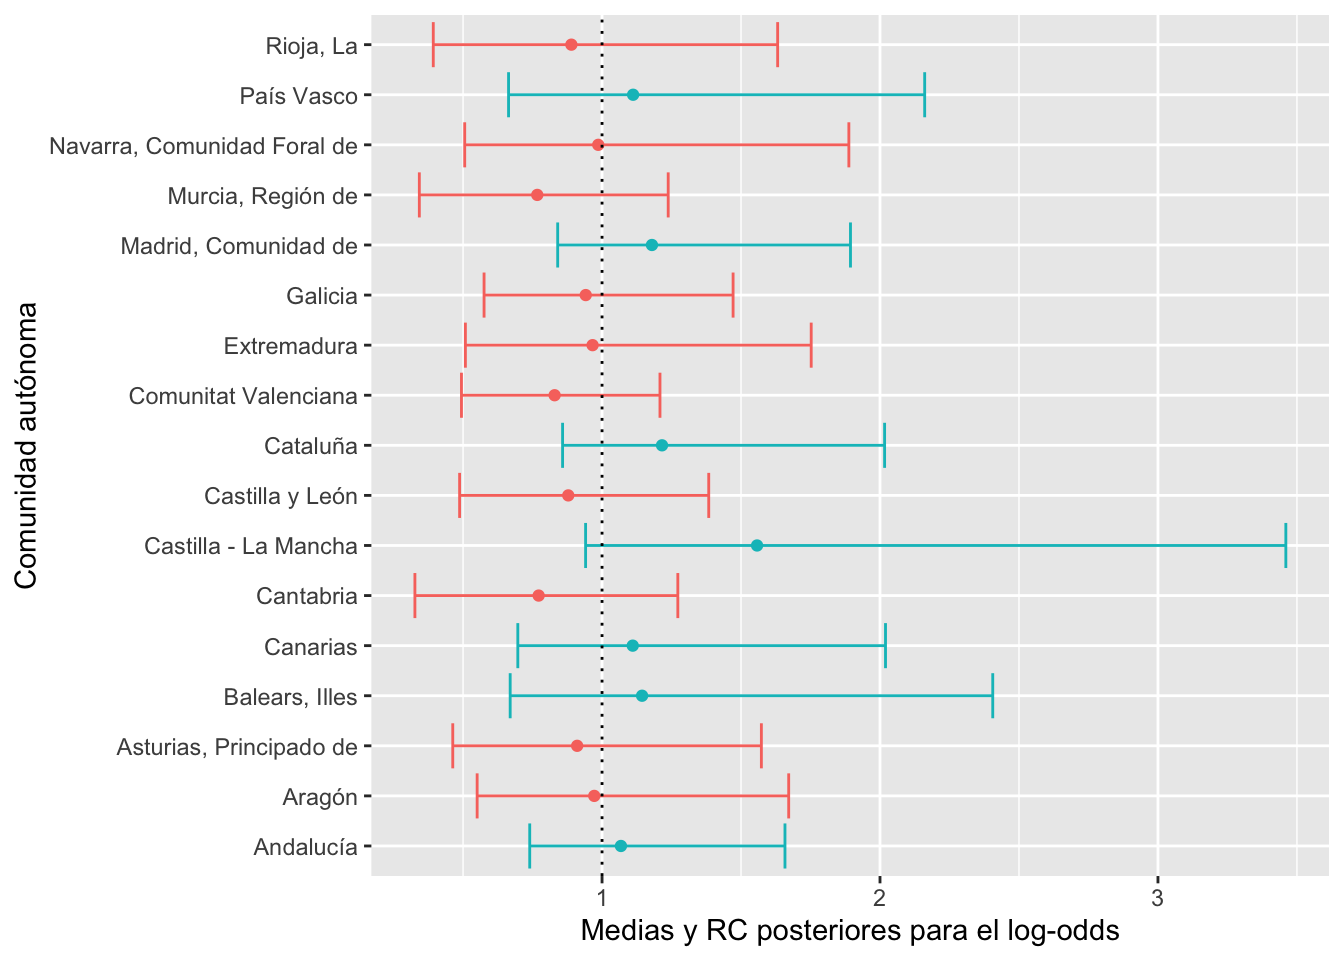
\includegraphics{03-glm_files/figure-latex/eleccion2-1.pdf}
\caption{\label{fig:eleccion2}Medias y RC posterioris para el log-odds de los efectos aleatorios}
\end{figure}

La distribución posterior de la probabilidad de voto para el PSOE para la comunidad con más variabilidad en el efecto aleatorio (Castilla-La Mancha), viene representada en la Figura \ref{fig:eleccion3} para las cuatro combinaciones posibles de valores para los predictores de simpatía y voto en el pasado.

\begin{Shaded}
\begin{Highlighting}[]
\NormalTok{datos\_pred }\OtherTok{=}\NormalTok{ datos }\SpecialCharTok{\%\textgreater{}\%}
  \FunctionTok{mutate}\NormalTok{(}\AttributeTok{f.post=}\FunctionTok{round}\NormalTok{(fit}\SpecialCharTok{$}\NormalTok{summary.fitted.values}\SpecialCharTok{$}\NormalTok{mean,}\DecValTok{3}\NormalTok{),}
        \AttributeTok{f.rc.low=}\FunctionTok{round}\NormalTok{(fit}\SpecialCharTok{$}\NormalTok{summary.fitted.values}\SpecialCharTok{$}\StringTok{"0.025quant"}\NormalTok{,}\DecValTok{3}\NormalTok{),}
         \AttributeTok{f.rc.up=}\FunctionTok{round}\NormalTok{(fit}\SpecialCharTok{$}\NormalTok{summary.fitted.values}\SpecialCharTok{$}\StringTok{"0.975quant"}\NormalTok{,}\DecValTok{3}\NormalTok{)) }\SpecialCharTok{\%\textgreater{}\%}
  \FunctionTok{distinct}\NormalTok{(f.post,}\AttributeTok{.keep\_all =} \ConstantTok{TRUE}\NormalTok{) }\SpecialCharTok{\%\textgreater{}\%}
  \FunctionTok{filter}\NormalTok{(ccaa}\SpecialCharTok{==}\StringTok{"Castilla {-} La Mancha"}\NormalTok{) }\SpecialCharTok{\%\textgreater{}\%}
  \FunctionTok{mutate}\NormalTok{(}\AttributeTok{simpast=}\FunctionTok{str\_c}\NormalTok{(psoe\_simp,psoe\_past))}
\FunctionTok{ggplot}\NormalTok{(datos\_pred,}\FunctionTok{aes}\NormalTok{(}\AttributeTok{x=}\NormalTok{f.post,}\AttributeTok{y=}\NormalTok{simpast))}\SpecialCharTok{+}
  \FunctionTok{geom\_point}\NormalTok{(}\FunctionTok{aes}\NormalTok{(}\AttributeTok{color=}\NormalTok{simpast))}\SpecialCharTok{+}
  \FunctionTok{geom\_errorbarh}\NormalTok{(}\FunctionTok{aes}\NormalTok{(}\AttributeTok{xmin=}\NormalTok{f.rc.low,}\AttributeTok{xmax=}\NormalTok{f.rc.up,}\AttributeTok{color=}\NormalTok{simpast),}\AttributeTok{height=}\FloatTok{0.2}\NormalTok{)}\SpecialCharTok{+}
  \FunctionTok{labs}\NormalTok{(}\AttributeTok{x=}\StringTok{"Medias y RC posteriores para la probabilidad de voto PSOE"}\NormalTok{,}\AttributeTok{title=}\StringTok{"Castilla {-} La Mancha"}\NormalTok{)}\SpecialCharTok{+}
  \FunctionTok{scale\_y\_discrete}\NormalTok{(}\AttributeTok{name=}\StringTok{""}\NormalTok{, }
                   \AttributeTok{labels=}\FunctionTok{c}\NormalTok{(}\StringTok{"No simpatía/No votó PSOE"}\NormalTok{,}\StringTok{"No simpatía/Votó PSOE"}\NormalTok{,}
                            \StringTok{"Simpatía/No votó PSOE"}\NormalTok{,}\StringTok{"Simpatía/Votó PSOE"}\NormalTok{))}\SpecialCharTok{+}
  \FunctionTok{theme}\NormalTok{(}\AttributeTok{legend.position=}\StringTok{"none"}\NormalTok{)}
\end{Highlighting}
\end{Shaded}

\begin{figure}
\centering
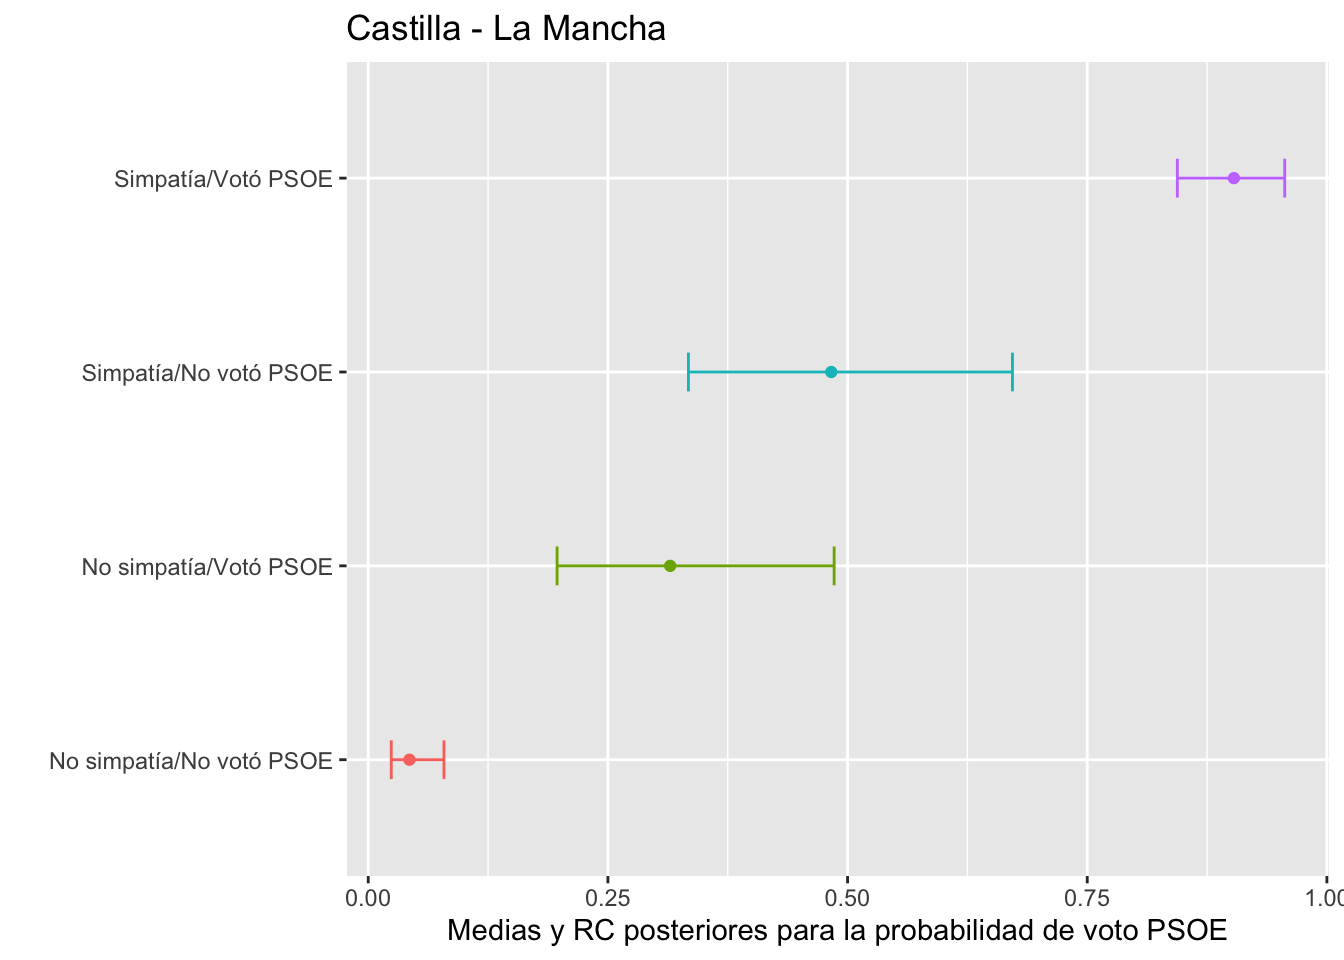
\includegraphics{03-glm_files/figure-latex/eleccion3-1.pdf}
\caption{\label{fig:eleccion3}Medias y RC posteriores para la probabilidad de voto PSOE}
\end{figure}

\hypertarget{mortalidad-por-infarto-en-sheffield}{%
\subsection{Mortalidad por infarto en Sheffield}\label{mortalidad-por-infarto-en-sheffield}}

Utilizamos los datos \emph{stroke}, disponibles en \href{https://sites.google.com/a/r-inla.org/stbook/datasets}{datasets in SSTM-RINLA}. Queremos evaluar la presencia de cierta asociación entre los niveles de NOx y el infarto en Sheffield, UK. Se dispone de la concentración anual de NOx medida en \(\mu g/m^3\) y categorizada en quintiles, promediada durante el periodo 1994-1999, en la variable \emph{NOx.class} y su análoga \(NOx\), y el número de muertes por infarto \(y\) en cada distrito identificado por el índice de desventajas y privación \emph{Townsend} (categorizado en quintiles). Se dispone igualmente del tamaño de la población para cada registro, en la variable \(pop\). La respuesta \(y\) se puede considerar entonces como conteos (de muertes) sobre la población de cada distrito,
\[y_i|\pi_i \sim Bin(n_i, \pi_i)\]
y el predictor lineal es función del nivel de NOx y del distrito:
\[\eta_i=logit(\pi_i)=\beta_0 + \sum_{k=2}^5 \beta_{1k} I(NOx_i=k)+ \sum_{h=2}^5 \beta_{2h} I(Townsend_i=h)+logit(\tilde{p_i})\]
siendo \(n_i\) la población (número total de habitantes) del distrito en el que se ubica el registro \(i\) (disponible en la variable \(pop\)). El término \(\tilde{p_i}\) representa el resgo ajustado por sexo y edad de la mortalidad por infarto, calculada utilizando estandarización indirecta con ratios de referencia internos basados en 18 estratos (9 para edad y 2 para género), y que se usa como un riesgo base en el modelo (Maheswaran et al.2006). En el ejemplo se calcula como el ratio de la mortalidad dividido por la población de cada registro.

\begin{Shaded}
\begin{Highlighting}[]
\NormalTok{url}\OtherTok{=}\StringTok{"https://raw.githubusercontent.com/BayesModel/data/main/Stroke.csv"}
\NormalTok{Stroke }\OtherTok{\textless{}{-}} \FunctionTok{read.csv}\NormalTok{(url,}\AttributeTok{sep=}\StringTok{","}\NormalTok{,}\AttributeTok{dec=}\StringTok{"."}\NormalTok{,}\AttributeTok{header=}\ConstantTok{TRUE}\NormalTok{)}
\CommentTok{\#riesgo base: ajuste por tamaño de la población}
\NormalTok{Stroke}\SpecialCharTok{$}\NormalTok{Adjusted.prob }\OtherTok{\textless{}{-}}\NormalTok{ Stroke}\SpecialCharTok{$}\NormalTok{stroke\_exp}\SpecialCharTok{/}\NormalTok{Stroke}\SpecialCharTok{$}\NormalTok{pop}
\CommentTok{\# logit del riesgo base}
\NormalTok{Stroke}\SpecialCharTok{$}\NormalTok{logit.adjusted.prob }\OtherTok{\textless{}{-}} \FunctionTok{log}\NormalTok{(Stroke}\SpecialCharTok{$}\NormalTok{Adjusted.prob}\SpecialCharTok{/}\NormalTok{(}\DecValTok{1}\SpecialCharTok{{-}}\NormalTok{Stroke}\SpecialCharTok{$}\NormalTok{Adjusted.prob))                          }
\end{Highlighting}
\end{Shaded}

Ajustamos ya el modelo, en el que las variables NOx y Townsend actúan como factores (efectos fijos) y el riesgo base se introduce como offset, para estandarizar los riesgos en función del tamaño de la población y poder equiparar así todos los distritos:

\begin{Shaded}
\begin{Highlighting}[]
\NormalTok{formula.inla }\OtherTok{\textless{}{-}}\NormalTok{ y }\SpecialCharTok{\textasciitilde{}} \DecValTok{1} \SpecialCharTok{+} \FunctionTok{factor}\NormalTok{(NOx) }\SpecialCharTok{+} \FunctionTok{factor}\NormalTok{(Townsend) }\SpecialCharTok{+} \FunctionTok{offset}\NormalTok{(logit.adjusted.prob)}
\NormalTok{model.logistic }\OtherTok{\textless{}{-}} \FunctionTok{inla}\NormalTok{(formula.inla, }\AttributeTok{family=}\StringTok{"binomial"}\NormalTok{, }\AttributeTok{Ntrials=}\NormalTok{pop, }\AttributeTok{data=}\NormalTok{Stroke)}
\FunctionTok{round}\NormalTok{(model.logistic}\SpecialCharTok{$}\NormalTok{summary.fixed[,}\DecValTok{1}\SpecialCharTok{:}\DecValTok{5}\NormalTok{],}\DecValTok{3}\NormalTok{)}
\CommentTok{\#\textgreater{}                     mean    sd 0.025quant 0.5quant}
\CommentTok{\#\textgreater{} (Intercept)       {-}0.181 0.057     {-}0.293   {-}0.180}
\CommentTok{\#\textgreater{} factor(NOx)2       0.132 0.059      0.016    0.132}
\CommentTok{\#\textgreater{} factor(NOx)3       0.105 0.061     {-}0.014    0.105}
\CommentTok{\#\textgreater{} factor(NOx)4       0.261 0.059      0.144    0.260}
\CommentTok{\#\textgreater{} factor(NOx)5       0.425 0.062      0.302    0.425}
\CommentTok{\#\textgreater{} factor(Townsend)2  0.077 0.061     {-}0.043    0.077}
\CommentTok{\#\textgreater{} factor(Townsend)3  0.137 0.060      0.020    0.137}
\CommentTok{\#\textgreater{} factor(Townsend)4 {-}0.132 0.063     {-}0.255   {-}0.132}
\CommentTok{\#\textgreater{} factor(Townsend)5 {-}0.118 0.067     {-}0.250   {-}0.118}
\CommentTok{\#\textgreater{}                   0.975quant}
\CommentTok{\#\textgreater{} (Intercept)           {-}0.071}
\CommentTok{\#\textgreater{} factor(NOx)2           0.248}
\CommentTok{\#\textgreater{} factor(NOx)3           0.225}
\CommentTok{\#\textgreater{} factor(NOx)4           0.377}
\CommentTok{\#\textgreater{} factor(NOx)5           0.547}
\CommentTok{\#\textgreater{} factor(Townsend)2      0.198}
\CommentTok{\#\textgreater{} factor(Townsend)3      0.255}
\CommentTok{\#\textgreater{} factor(Townsend)4     {-}0.009}
\CommentTok{\#\textgreater{} factor(Townsend)5      0.014}
\end{Highlighting}
\end{Shaded}

Para obtener la probabilidad promedio de muerte por infarto en el distrito Townsend=1 y para el nivel NOx=1, que son los niveles base, nos apoyamos en la interceptación \(\beta_0\). Sobre sus simulaciones será preciso deshacer el logit (con la función logit-inversa):

\begin{Shaded}
\begin{Highlighting}[]
\NormalTok{prob.stroke }\OtherTok{\textless{}{-}} \FunctionTok{inla.tmarginal}\NormalTok{(}\ControlFlowTok{function}\NormalTok{(x) }\FunctionTok{exp}\NormalTok{(x)}\SpecialCharTok{/}\NormalTok{(}\DecValTok{1}\SpecialCharTok{+}\FunctionTok{exp}\NormalTok{(x)), model.logistic}\SpecialCharTok{$}\NormalTok{marginals.fixed[[}\DecValTok{1}\NormalTok{]])}
\FunctionTok{inla.zmarginal}\NormalTok{(prob.stroke)}
\CommentTok{\#\textgreater{} Mean            0.455034 }
\CommentTok{\#\textgreater{} Stdev           0.0139168 }
\CommentTok{\#\textgreater{} Quantile  0.025 0.427486 }
\CommentTok{\#\textgreater{} Quantile  0.25  0.445615 }
\CommentTok{\#\textgreater{} Quantile  0.5   0.455082 }
\CommentTok{\#\textgreater{} Quantile  0.75  0.464485 }
\CommentTok{\#\textgreater{} Quantile  0.975 0.482137}
\FunctionTok{ggplot}\NormalTok{(}\FunctionTok{data.frame}\NormalTok{(prob.stroke),}\FunctionTok{aes}\NormalTok{(}\AttributeTok{x=}\NormalTok{x,}\AttributeTok{y=}\NormalTok{y))}\SpecialCharTok{+}\FunctionTok{geom\_line}\NormalTok{()}\SpecialCharTok{+}
         \FunctionTok{labs}\NormalTok{(}\AttributeTok{x=}\FunctionTok{expression}\NormalTok{(pi),}\AttributeTok{y=} \FunctionTok{expression}\NormalTok{(}\FunctionTok{tilde}\NormalTok{(p)(}\FunctionTok{paste}\NormalTok{(pi,}\StringTok{"|"}\NormalTok{,y,}\StringTok{","}\NormalTok{,NOx[}\DecValTok{1}\NormalTok{],}\StringTok{","}\NormalTok{,TS[}\DecValTok{1}\NormalTok{]))))}
\end{Highlighting}
\end{Shaded}

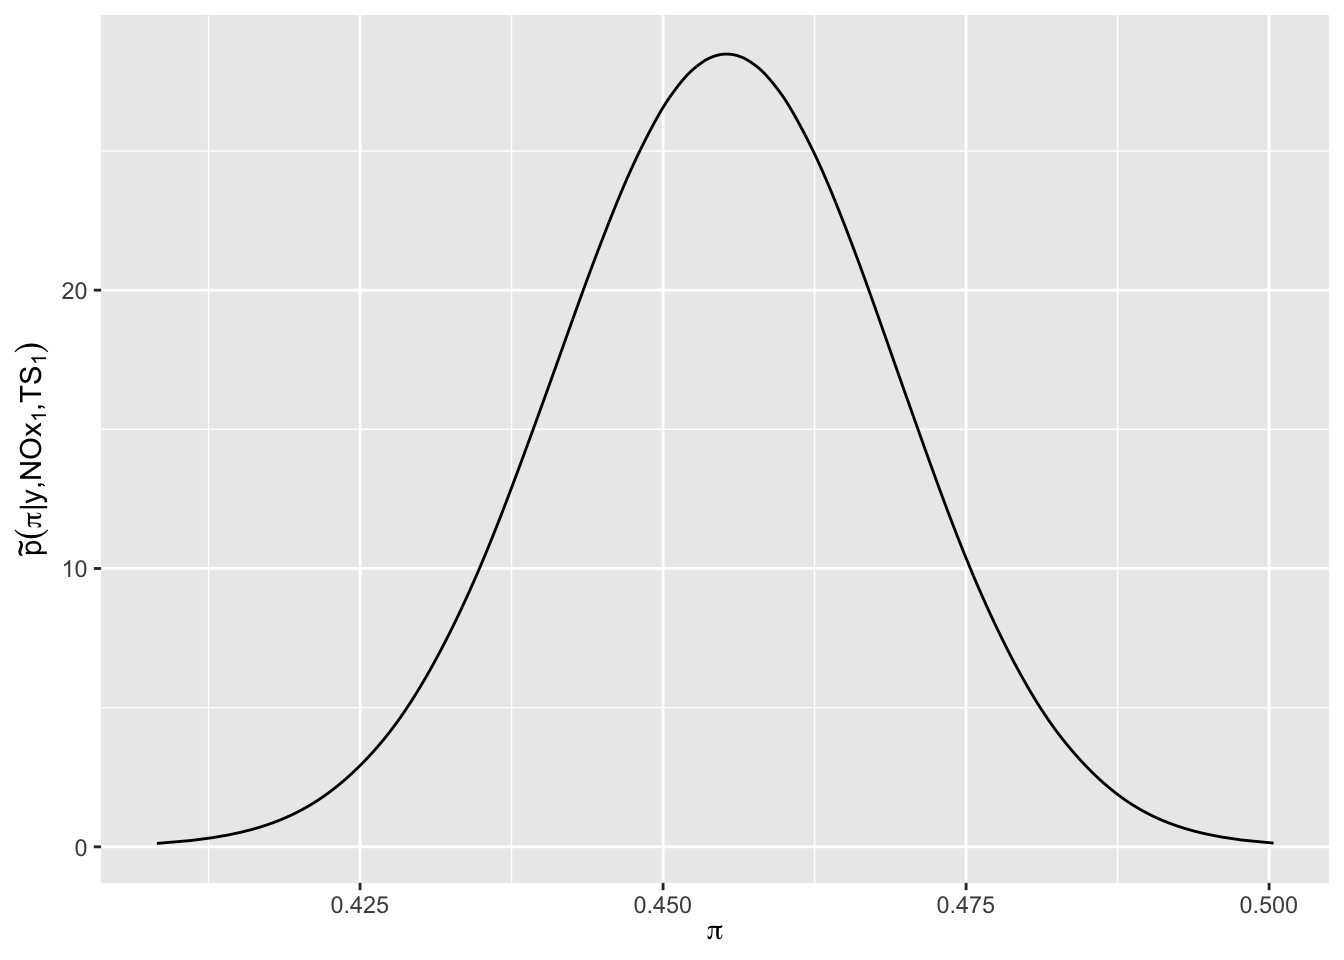
\includegraphics{03-glm_files/figure-latex/unnamed-chunk-6-1.pdf}

El efecto \(\beta_{12}\) representa el efecto en los log.odds de la mortalidad por infarto de estar en el nivel \(NOx=2\) frente al de estar en el nivel \(NOx=1\). Si queremos evaluar el odds-ratio, simplemente calculamos la distribución posterior de \(exp(\beta_{12})\) con \texttt{inla.tmarginal}. Si sólo estamos interesados en su media, bastaría utilizar `inla.emarginal':

\begin{Shaded}
\begin{Highlighting}[]
\NormalTok{odds.nox21 }\OtherTok{\textless{}{-}} \FunctionTok{inla.tmarginal}\NormalTok{(}\ControlFlowTok{function}\NormalTok{(x) }\FunctionTok{exp}\NormalTok{(x), model.logistic}\SpecialCharTok{$}\NormalTok{marginals.fixed}\SpecialCharTok{$}\StringTok{"factor(NOx)2"}\NormalTok{)}
\NormalTok{e}\OtherTok{\textless{}{-}}\FunctionTok{inla.emarginal}\NormalTok{(exp, model.logistic}\SpecialCharTok{$}\NormalTok{marginals.fixed}\SpecialCharTok{$}\StringTok{"factor(NOx)2"}\NormalTok{)}
\FunctionTok{ggplot}\NormalTok{(}\FunctionTok{data.frame}\NormalTok{(odds.nox21),}\FunctionTok{aes}\NormalTok{(}\AttributeTok{x=}\NormalTok{x,}\AttributeTok{y=}\NormalTok{y))}\SpecialCharTok{+}\FunctionTok{geom\_line}\NormalTok{()}\SpecialCharTok{+}
        \FunctionTok{labs}\NormalTok{(}\AttributeTok{x=}\FunctionTok{expression}\NormalTok{(}\FunctionTok{OR}\NormalTok{(NOx[}\DecValTok{21}\NormalTok{])),}\AttributeTok{y=} \FunctionTok{expression}\NormalTok{(}\FunctionTok{tilde}\NormalTok{(p)(}\FunctionTok{paste}\NormalTok{(}\FunctionTok{OR}\NormalTok{(NOx[}\DecValTok{21}\NormalTok{]),}\StringTok{"|"}\NormalTok{,y))))}\SpecialCharTok{+}
        \FunctionTok{geom\_vline}\NormalTok{(}\AttributeTok{xintercept=}\NormalTok{e,}\AttributeTok{color=}\StringTok{"pink"}\NormalTok{)}\SpecialCharTok{+} \FunctionTok{geom\_text}\NormalTok{(}\AttributeTok{x=}\NormalTok{e,}\AttributeTok{y=}\DecValTok{1}\NormalTok{,}\AttributeTok{label=}\FunctionTok{paste}\NormalTok{(}\StringTok{"mean="}\NormalTok{,}\FunctionTok{round}\NormalTok{(e,}\DecValTok{3}\NormalTok{)),}\AttributeTok{color=}\StringTok{"red"}\NormalTok{)}
\end{Highlighting}
\end{Shaded}

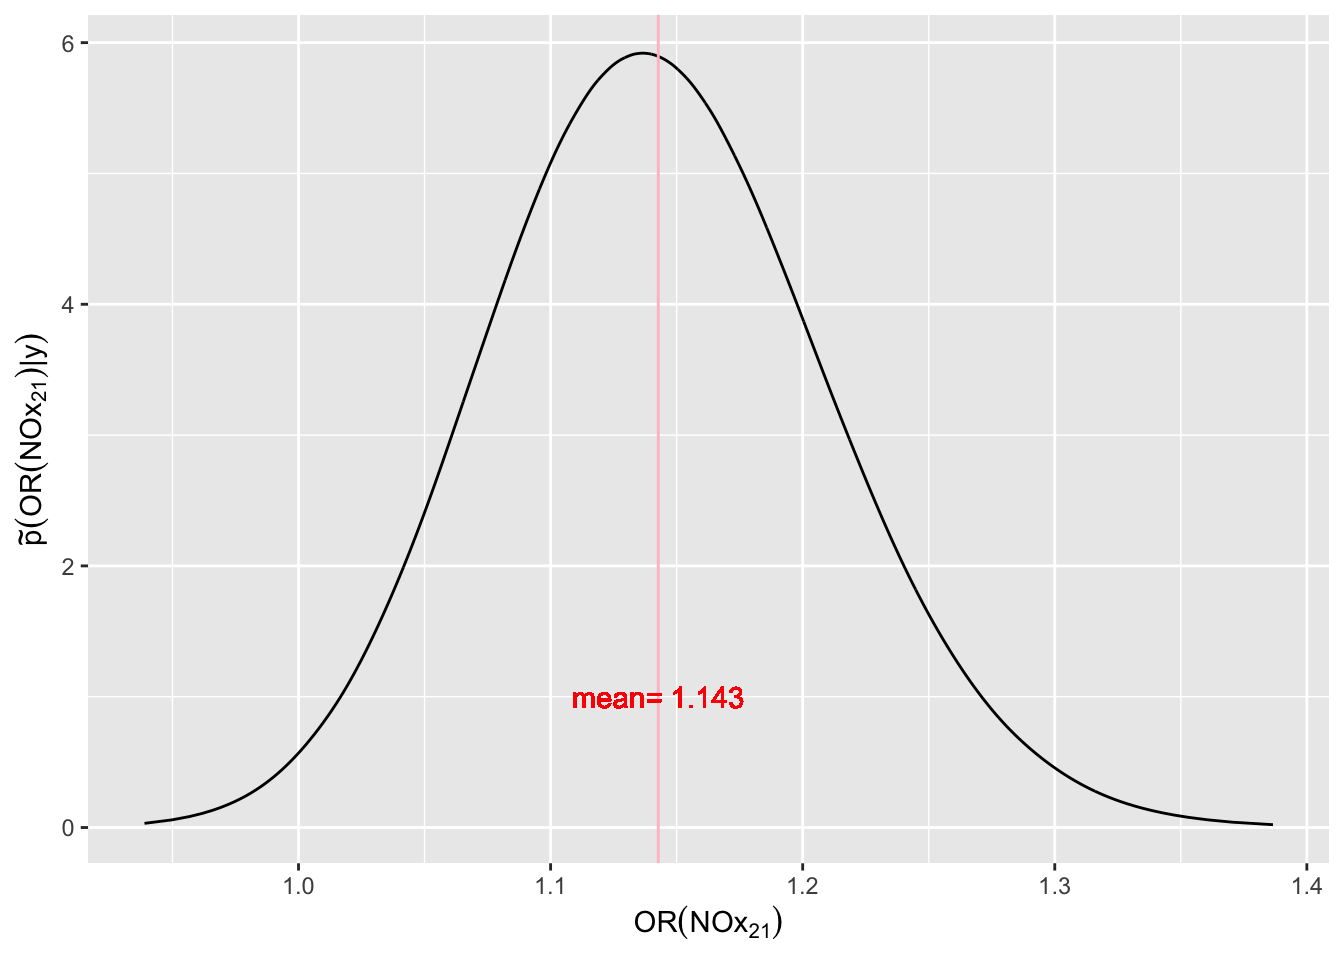
\includegraphics{03-glm_files/figure-latex/unnamed-chunk-7-1.pdf}

La probabilidad de muerte por infarto se incrementa en un 14.3\% cuando la exposición de NOx cambia del primer al segundo nivel. Los odds-ratio para el resto de los niveles resultan realmente significativos: 11,3\% el odds-ratio NOx3/NOx1, 30\% NOx4/NOx1 y 53.2\% NOx5/NOx1.

\begin{Shaded}
\begin{Highlighting}[]
\FunctionTok{inla.emarginal}\NormalTok{(exp, model.logistic}\SpecialCharTok{$}\NormalTok{marginals.fixed}\SpecialCharTok{$}\StringTok{"factor(NOx)3"}\NormalTok{)}
\CommentTok{\#\textgreater{} [1] 1.113128}
\FunctionTok{inla.emarginal}\NormalTok{(exp, model.logistic}\SpecialCharTok{$}\NormalTok{marginals.fixed}\SpecialCharTok{$}\StringTok{"factor(NOx)4"}\NormalTok{)}
\CommentTok{\#\textgreater{} [1] 1.299909}
\FunctionTok{inla.emarginal}\NormalTok{(exp, model.logistic}\SpecialCharTok{$}\NormalTok{marginals.fixed}\SpecialCharTok{$}\StringTok{"factor(NOx)5"}\NormalTok{)}
\CommentTok{\#\textgreater{} [1] 1.532265}
\end{Highlighting}
\end{Shaded}

\hypertarget{regresiuxf3n-de-poisson}{%
\section{Regresión de Poisson}\label{regresiuxf3n-de-poisson}}

La regresión de Poisson es útil cuando la variable respuesta representa conteos y estos toman valores discretos entre 0 y \(+\infty\), sin una cota superior de referencia. El parámetro de interés es el número promedio de eventos \(\lambda=E(y)\) y el link natural es el logaritmo, de modo que el predictor lineal está ligado con las covariables y factores según:
\[\eta=log(\lambda)=x \beta, \ \ \mbox{ y } \ \ \lambda_i=exp(X \beta)\]

Un modelo de Poisson puede especificarse según
\[y_i \sim Po(\lambda_i), i=1,...,n\]
\[\eta_i=log(\lambda_i)=\beta_0+\sum_{m=1}^M \beta_mx_{im}.\]

Para completar el modelo se especifican distribuciones a priori para \(\beta\), típicamente como normales con media cero y una varianza grande cuando no hay información disponible de estudios previos u opinión de expertos.

Los coeficientes se interpretan a través de la función exponencial:

\begin{itemize}
\tightlist
\item
  \(exp(\beta_0)=\lambda_i\) cuando todas las \(x=0\) si son continuas, o para el primer nivel de las categorías posibles si son categóricas.
\item
  \(exp(\beta_m)\) es el cambio que se produce en la respuesta promedio \(y\) cuando \(x_m\) se incrementa en una unidad.
\end{itemize}

La mayoría de las veces que se utiliza la regresión de Poisson, el interés recáe en las ratios o riesgos relativos, más que en el número promedio de casos \(\lambda_i\). Para cambiar la escala en términos de riesgo, ha de utilizarse un offset como factor de corrección en la especificación del modelo. Este offset representa el denominador del riesgo y entra en la regresión en una escala logarítmica, asumiendo que tiene un coeficiente de regresión fijado a 1:
\[\eta_i=log(\lambda_i)=\beta_0+\sum_{m=1}^M \beta_mx_{im}+log(Offset_i)\]
donde el riesgo relativo de que se produzca un evento se obtiene según
\[log\left(\frac{\lambda_i}{Offset_i}\right)=\beta_0+\sum_{m=1}^M \beta_mx_{im}\]
y los coeficientes entonces se interpretan en una escala de riesgo. En este caso al exponenciar la interceptación obtenemos el riesgo base, mientras que \(exp(\beta_m)\) representa el cambio en el riesgo relativo debido a un cambio de unidad en el predictor correspondiente.

\hypertarget{incidentes-en-barcos}{%
\subsection{Incidentes en barcos}\label{incidentes-en-barcos}}

Utilizamos los datos \emph{ships.csv} en \href{https://sites.google.com/a/r-inla.org/stbook/datasets}{datasets for SSTM-RINLA} para estimar el riesgo mensual de incidentes en barcos. Los factores potenciales del riesgo son el periodo de construcción (\emph{built}), el periodo de operación (\emph{oper}) y el tipo de barco (\emph{type}).
El modelo se escribe en INLA a continuación, utilizando como offset el \emph{log(months)}, que son los meses que ha navegado y ponderan en consecuencia el riesgo de incidentes. El modelo con el offset será entonces
\[y_i \sim Poisson (E_i \rho_i),\]
donde \(\eta_i=log(\rho_i)\) es el predictor lineal y el promedio del número de incidentes \(\lambda_i=E_i \rho_i\). El offset no se incluye en esta formulación en el predictor lineal.

\begin{Shaded}
\begin{Highlighting}[]
\NormalTok{url}\OtherTok{=}\StringTok{"https://raw.githubusercontent.com/BayesModel/data/main/Ships.csv"}
\NormalTok{ShipsIncidents }\OtherTok{\textless{}{-}} \FunctionTok{read.csv}\NormalTok{(url,}\AttributeTok{sep=}\StringTok{","}\NormalTok{) }

\NormalTok{formula.inla }\OtherTok{\textless{}{-}}\NormalTok{ y }\SpecialCharTok{\textasciitilde{}} \DecValTok{1} \SpecialCharTok{+}\NormalTok{ built }\SpecialCharTok{+}\NormalTok{ oper }\SpecialCharTok{+}\NormalTok{ type}
\NormalTok{model.poisson }\OtherTok{\textless{}{-}} \FunctionTok{inla}\NormalTok{(formula.inla,}\AttributeTok{family=}\StringTok{"poisson"}\NormalTok{, }\AttributeTok{data=}\NormalTok{ShipsIncidents, }\AttributeTok{offset=}\FunctionTok{log}\NormalTok{(months))}

\FunctionTok{round}\NormalTok{(model.poisson}\SpecialCharTok{$}\NormalTok{summary.fixed[,}\DecValTok{1}\SpecialCharTok{:}\DecValTok{5}\NormalTok{],}\DecValTok{3}\NormalTok{)}
\CommentTok{\#\textgreater{}               mean    sd 0.025quant 0.5quant 0.975quant}
\CommentTok{\#\textgreater{} (Intercept) {-}6.416 0.217     {-}6.852   {-}6.413     {-}5.998}
\CommentTok{\#\textgreater{} built65{-}69   0.696 0.150      0.406    0.695      0.994}
\CommentTok{\#\textgreater{} built70{-}74   0.819 0.170      0.487    0.818      1.153}
\CommentTok{\#\textgreater{} built75{-}79   0.453 0.233     {-}0.012    0.455      0.903}
\CommentTok{\#\textgreater{} oper75{-}79    0.384 0.118      0.153    0.384      0.617}
\CommentTok{\#\textgreater{} typeB       {-}0.543 0.178     {-}0.882   {-}0.546     {-}0.185}
\CommentTok{\#\textgreater{} typeC       {-}0.688 0.329     {-}1.366   {-}0.678     {-}0.075}
\CommentTok{\#\textgreater{} typeD       {-}0.075 0.291     {-}0.664   {-}0.069      0.476}
\CommentTok{\#\textgreater{} typeE        0.326 0.236     {-}0.141    0.327      0.785}
\end{Highlighting}
\end{Shaded}

\begin{Shaded}
\begin{Highlighting}[]
\FunctionTok{names}\NormalTok{(model.poisson}\SpecialCharTok{$}\NormalTok{marginals.fixed)}
\CommentTok{\#\textgreater{} [1] "(Intercept)" "built65{-}69"  "built70{-}74"  "built75{-}79" }
\CommentTok{\#\textgreater{} [5] "oper75{-}79"   "typeB"       "typeC"       "typeD"      }
\CommentTok{\#\textgreater{} [9] "typeE"}
\CommentTok{\# ratio medio de incidentes por mes en las categorías base}
\FunctionTok{inla.emarginal}\NormalTok{(exp,model.poisson}\SpecialCharTok{$}\NormalTok{marginals.fixed[[}\DecValTok{1}\NormalTok{]])}
\CommentTok{\#\textgreater{} [1] 0.001674164}
\CommentTok{\# riesgo relativo de barcos tipo E}
\FunctionTok{inla.emarginal}\NormalTok{(exp,model.poisson}\SpecialCharTok{$}\NormalTok{marginals.fixed}\SpecialCharTok{$}\NormalTok{typeE)}
\CommentTok{\#\textgreater{} [1] 1.424414}
\end{Highlighting}
\end{Shaded}

Así, la media de \(exp(\beta_0)\), 0.0018, representa el ratio medio de incidentes por mes entre los barcos que fueron construidos entre el 60 y el 64, han operado entre el 60 y el 74 y son de tipo A (las categorías de referencia). El ratio en 1000 meses sería del 1.8.Para los barcos de tipo E el incremento en el ratio mensual de incidentes, comparado con los de tipo A es del 42,4\%.

Otros datos modelizables con una regresión de Poisson son los que provienen del libro de Andrews and Herzberg y están descritos en (\href{http://www.randomservices.org/random/data/HorseKicks.html}{randomservices.org/random}) consistentes en el número de soldados muertos por coces de caballo en diversos cuerpos de caballería del ejército prusiano, entre 1875 y 1894.

Este modelo se implementa en INLA, a partir de datos simulados, con el siguiente código

\begin{Shaded}
\begin{Highlighting}[]
\NormalTok{url}\OtherTok{=}\StringTok{"https://raw.githubusercontent.com/BayesModel/data/main/HorseKicks.txt"}
\NormalTok{horse}\OtherTok{\textless{}{-}}\FunctionTok{read.csv}\NormalTok{(url,}\AttributeTok{sep=}\StringTok{""}\NormalTok{, }\AttributeTok{dec=}\StringTok{"."}\NormalTok{,}\AttributeTok{header=}\ConstantTok{TRUE}\NormalTok{)}
\NormalTok{horse}\SpecialCharTok{$}\NormalTok{sum}\OtherTok{\textless{}{-}}\FunctionTok{apply}\NormalTok{(horse[,}\DecValTok{2}\SpecialCharTok{:}\FunctionTok{ncol}\NormalTok{(horse)],}\DecValTok{1}\NormalTok{,sum)}

\NormalTok{fit}\OtherTok{=}\FunctionTok{inla}\NormalTok{(sum}\SpecialCharTok{\textasciitilde{}}\DecValTok{1}\NormalTok{,}\AttributeTok{data=}\NormalTok{horse,}\AttributeTok{family=}\StringTok{"poisson"}\NormalTok{,}\AttributeTok{control.predictor=}\FunctionTok{list}\NormalTok{(}\AttributeTok{compute=}\ConstantTok{TRUE}\NormalTok{))}
\FunctionTok{summary}\NormalTok{(fit)}
\CommentTok{\#\textgreater{} }
\CommentTok{\#\textgreater{} Call:}
\CommentTok{\#\textgreater{}    c("inla.core(formula = formula, family = family, }
\CommentTok{\#\textgreater{}    contrasts = contrasts, ", " data = data, quantiles = }
\CommentTok{\#\textgreater{}    quantiles, E = E, offset = offset, ", " scale = }
\CommentTok{\#\textgreater{}    scale, weights = weights, Ntrials = Ntrials, strata = }
\CommentTok{\#\textgreater{}    strata, ", " lp.scale = lp.scale, link.covariates = }
\CommentTok{\#\textgreater{}    link.covariates, verbose = verbose, ", " lincomb = }
\CommentTok{\#\textgreater{}    lincomb, selection = selection, control.compute = }
\CommentTok{\#\textgreater{}    control.compute, ", " control.predictor = }
\CommentTok{\#\textgreater{}    control.predictor, control.family = control.family, }
\CommentTok{\#\textgreater{}    ", " control.inla = control.inla, control.fixed = }
\CommentTok{\#\textgreater{}    control.fixed, ", " control.mode = control.mode, }
\CommentTok{\#\textgreater{}    control.expert = control.expert, ", " control.hazard }
\CommentTok{\#\textgreater{}    = control.hazard, control.lincomb = control.lincomb, }
\CommentTok{\#\textgreater{}    ", " control.update = control.update, }
\CommentTok{\#\textgreater{}    control.lp.scale = control.lp.scale, ", " }
\CommentTok{\#\textgreater{}    control.pardiso = control.pardiso, only.hyperparam = }
\CommentTok{\#\textgreater{}    only.hyperparam, ", " inla.call = inla.call, inla.arg }
\CommentTok{\#\textgreater{}    = inla.arg, num.threads = num.threads, ", " }
\CommentTok{\#\textgreater{}    blas.num.threads = blas.num.threads, keep = keep, }
\CommentTok{\#\textgreater{}    working.directory = working.directory, ", " silent = }
\CommentTok{\#\textgreater{}    silent, inla.mode = inla.mode, safe = FALSE, debug = }
\CommentTok{\#\textgreater{}    debug, ", " .parent.frame = .parent.frame)") }
\CommentTok{\#\textgreater{} Time used:}
\CommentTok{\#\textgreater{}     Pre = 2.26, Running = 0.165, Post = 0.00703, Total = 2.43 }
\CommentTok{\#\textgreater{} Fixed effects:}
\CommentTok{\#\textgreater{}              mean    sd 0.025quant 0.5quant 0.975quant mode}
\CommentTok{\#\textgreater{} (Intercept) 2.282 0.071      2.139    2.283       2.42   NA}
\CommentTok{\#\textgreater{}             kld}
\CommentTok{\#\textgreater{} (Intercept)   0}
\CommentTok{\#\textgreater{} }
\CommentTok{\#\textgreater{} Marginal log{-}Likelihood:  {-}61.30 }
\CommentTok{\#\textgreater{}  is computed }
\CommentTok{\#\textgreater{} Posterior summaries for the linear predictor and the fitted values are computed}
\CommentTok{\#\textgreater{} (Posterior marginals needs also \textquotesingle{}control.compute=list(return.marginals.predictor=TRUE)\textquotesingle{})}
\end{Highlighting}
\end{Shaded}


  \bibliography{book.bib,packages.bib}

\end{document}
